\documentclass[tcc,capa]{texufpel}

\usepackage[utf8]{inputenc} % acentuacao
\usepackage{graphicx} % para inserir figuras
\usepackage[T1]{fontenc}
\usepackage[ruled,vlined]{algorithm2e}
\usepackage{longtable}
\usepackage{pdfpages}

\hypersetup{
    hidelinks, % Remove coloração e caixas
    unicode=true,   %Permite acentuação no bookmark
    linktoc=all %Habilita link no nome e página do sumário
}

\unidade{Centro de Desenvolvimento Tecnológico}
\curso{Ciência da Computação}
\nomecurso{Bacharelado em Ciência da Computação}
\titulocurso{Bacharel em Ciência da Computação}

\unidadeeng{Technology Development Center}
\cursoeng{Computer Science}


\title{Plataforma Web para Monitoramento de Dados Oriundos de Redes de Sensores sem Fio}

\author{Huber}{Mathaus Corrêa}
\advisor[Prof.~Dr.]{Marques}{Felipe de Souza}
\coadvisor[Prof.~Dr.]{Corrêa}{Ulisses Brisolara}

%Palavras-chave em PT_BR
\keyword{Aplicação Web}
\keyword{Plataforma IoT}
\keyword{Software de gestão}
\keyword{Sistema Computacional}

%Palavras-chave em EN_US
\keywordeng{Web Application}
\keywordeng{IoT Platform}
\keywordeng{Management software}
\keywordeng{Computer System}

\begin{document}

\renewcommand{\advisorname}{Orientador}           %descomente caso tenhas orientadora
\renewcommand{\coadvisorname}{Coorientador}      %descomente caso tenhas coorientadora

\maketitle 

\sloppy

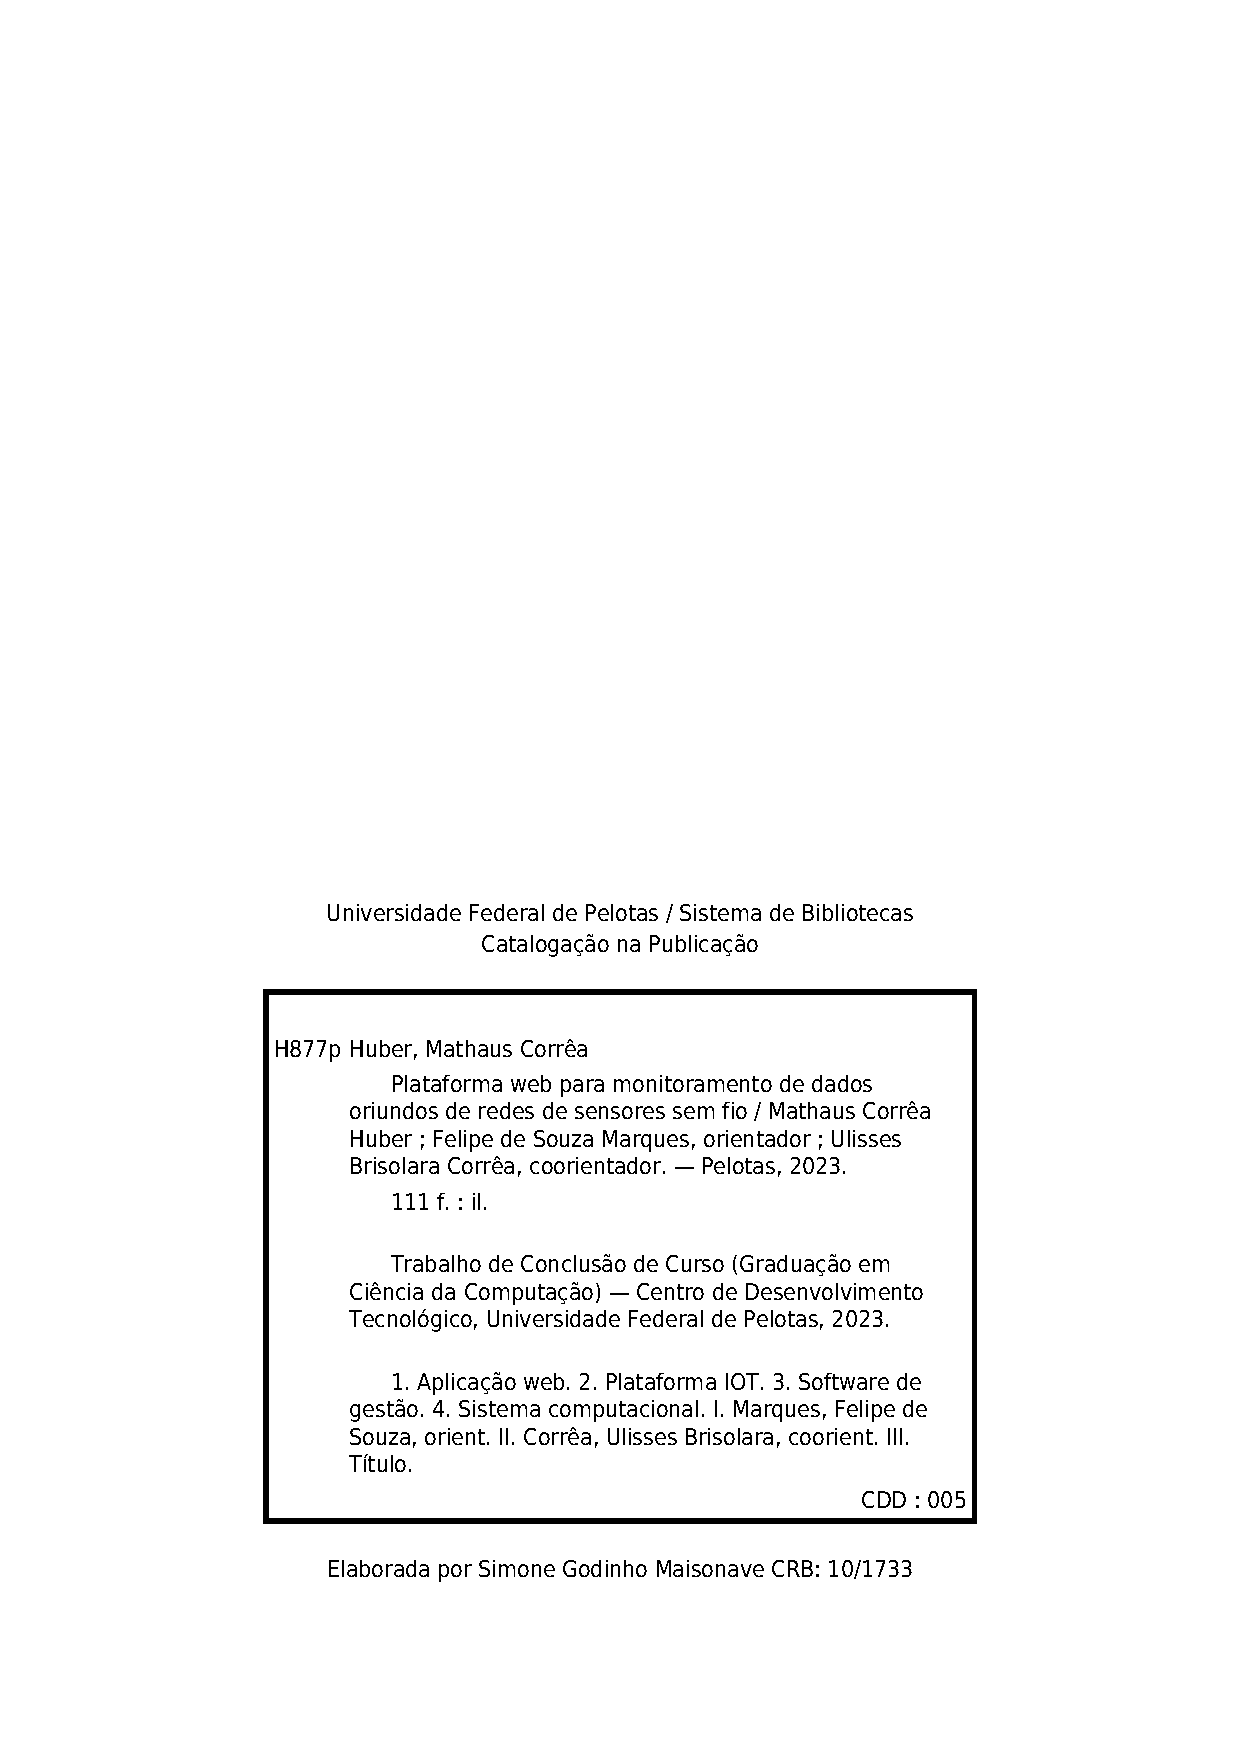
\includepdf{ficha.pdf}

%\folhadeaprovacao

%Composição da Banca Examinadora
\begin{aprovacao}{11 de maio de 2023} %data da banca por extenso
    \noindent Prof. Dr. Felipe de Souza Marques (orientador)\\
Doutor em Ciência da Computação pela Universidade Federal do Rio Grande do Sul.\\[1cm]

\noindent Prof. Dr. Ulisses Brisolara Corrêa (coorientador)\\
Doutor em Ciência da Computação pela Universidade Federal de Pelotas.\\[1cm]

\noindent Profa. Dra. Lisane Brisolara de Brisolara \\
Doutora em Ciência da Computação pela Universidade Federal do Rio Grande do Sul.\\[1cm]

\noindent Prof. Dr. Guilherme Tomaschewski Netto \\
Doutor em Oceanologia pela Universidade Federal do Rio Grande.\\[1cm]


\end{aprovacao}

%Opcional
\begin{dedicatoria}
  Dedico este trabalho a mim mesmo, por ter tido a força e a determinação necessárias para estudar e trabalhar ao mesmo tempo durante a graduação, e por ter enfrentado com coragem e resiliência os desafios de morar fora da minha cidade. Este trabalho representa não apenas uma conquista acadêmica, mas também uma prova de que, com esforço e dedicação, é possível alcançar nossos objetivos.

Também dedico este trabalho aos meus pais, que sempre me apoiaram e incentivaram em todas as etapas da minha vida. Sem o seu suporte emocional e financeiro, eu não teria conseguido concluir esta etapa tão importante da minha formação acadêmica. Agradeço de coração por tudo o que fizeram por mim.

Que este trabalho possa inspirar e motivar outras pessoas a perseverar em busca de seus sonhos, mesmo diante dos desafios e obstáculos que a vida nos apresenta.
\end{dedicatoria}

%Opcional
\begin{agradecimentos}
  É com grande satisfação que concluo este trabalho e gostaria de expressar minha gratidão a todas as pessoas que contribuíram para a sua realização. Em especial, gostaria de agradecer aos meus pais, minha namorada e minha dinda, que sempre estiveram presentes, me apoiando e incentivando em todas as etapas da minha vida. Seu amor e suporte foram fundamentais para que eu pudesse chegar até aqui.

Agradeço também aos meus orientadores, Felipe de Souza Marques e Ulisses Brisolara Corrêa, que me guiaram com dedicação, paciência e sabedoria durante todo o processo de pesquisa e escrita deste trabalho. Sem o seu conhecimento e orientação, eu não teria conseguido atingir meus objetivos.

Não posso deixar de agradecer aos professores da Universidade Federal de Pelotas, em especial ao professor Rafael Torchelsen e André Rauber Du Bois, cujas aulas, palestras e orientações foram essenciais para o meu aprendizado e desenvolvimento acadêmico. Agradeço por compartilharem seus conhecimentos e experiências.

Também quero expressar minha gratidão à minha dinda, que me acolheu em sua casa durante a graduação e me permitiu focar nos estudos e na pesquisa. Sua generosidade e apoio foram fundamentais para o meu sucesso acadêmico.

Por fim, gostaria de agradecer a todos os amigos e familiares que me apoiaram, incentivaram e motivaram ao longo desta jornada. Sua presença em minha vida é muito importante e não posso deixar de mencionar a importância de cada um de vocês.

Este trabalho representa não apenas um marco importante em minha trajetória acadêmica, mas também um processo de aprendizado e crescimento pessoal. A todos que contribuíram para essa realização, meu muito obrigado!

\end{agradecimentos}

%Opcional
\begin{epigrafe}
  Per aspera ad astra.\\
  {\sc --- Provérbio Latino}
\end{epigrafe}

%Resumo em Portugues (no maximo 500 palavras)
\begin{abstract}
Embora a ideia de IoT já exista há muito tempo, uma série de avanços tecnológicos recentes em algumas áreas tornou-a possível em termos práticos. Com esse conceito, através dos dados gerados podemos transformá-los em informação valorável para os seres humanos com a conectividade de dispositivos usando a internet como canal comum.

Dessa forma, este trabalho detalha o desenvolvimento de uma aplicação web capaz de apresentar informações estruturadas a partir de dashboards, que consideram dados oriundos de diferentes tipos de Redes de Sensores sem Fio (RSSF) aplicadas a smartfarms, smartcities, smartcampus, etc. A plataforma disponibilizará APIs para os usuários cadastrados, permitindo a configuração de um dashboard para monitorar dados de diferentes tipos de sensores, incluindo a possibilidade de monitoramento de dados de telemetria. A partir da disponibilização destas funcionalidades em uma plataforma web, almeja-se garantir um fluxo constante de dados, que darão origem a séries históricas para que sejam realizadas análises preditivas.

A validação inicial da plataforma ocorre por meio de dois estudos de caso: um dentro do campus anglo da Universidade Federal de Pelotas, utilizando uma rede de sensores em desenvolvimento pelo grupo de pesquisa do proponente, e outro em parceria com a ALM (Agência de Desenvolvimento da Bacia da Lagoa Mirim), visando o monitoramento de estações hidrológicas e meteorológicas na região da bacia da Lagoa Mirim. Essas escolhas estratégicas permitem avaliar a integração e confiabilidade da plataforma, bem como sua capacidade em lidar com dados de múltiplas fontes e potencial para uso em larga escala, evidenciando sua utilidade em aplicações reais e acadêmicas.
\end{abstract}

%Resumo em Inglês (no maximo 500 palavras)
\begin{englishabstract}{Web Platform for Monitoring Sourced Data of Wireless Sensor Networks}
Although the idea of IoT has existed for a long time, a series of recent technological advancements in some areas have made it possible in practical terms. With this concept, we can transform generated data into valuable information for humans with the connectivity of devices using the internet as a common channel.

Thus, this work details the development of a web application capable of presenting structured information from dashboards that consider data from different types of Wireless Sensor Networks (WSN) applied to smart farms, smart cities, smart campuses, etc. The platform will provide APIs for registered users, allowing for the configuration of a dashboard to monitor data from different types of sensors, including the possibility of telemetry data monitoring. By providing these functionalities on a web platform, the aim is to ensure a constant flow of data, which will give rise to historical series for predictive analysis.

The initial validation of the platform occurs through two case studies: one within the Anglo campus of the Federal University of Pelotas, using a sensor network under development by the proponent's research group, and another in partnership with ALM (Agency for the Development of the Lagoa Mirim Basin), aiming at monitoring hydrological and meteorological stations in the region of the Lagoa Mirim basin. These strategic choices allow for the evaluation of the integration and reliability of the platform, as well as its ability to handle data from multiple sources and its potential for use on a large scale, demonstrating its usefulness in real and academic applications.
\end{englishabstract}

%Lista de Figuras
\listoffigures

%Lista de Tabelas
\listoftables

%lista de abreviaturas e siglas
\begin{listofabbrv}{EMBRAPA}%coloque aqui a maior sigla para ajustar a distância
        \item[EMBRAPA] Empresa Brasileira de Pesquisa Agropecuária
        \item[API] Application Programming Interface
        \item[RSSF] Rede de Sensores sem Fio
        \item[IoT] Internet of Things
        \item[UI] User Interface
        \item[UX] User Experience
        \item[HTML] Hypertext Markup Language
        \item[CSS] Cascading Style Sheets
        \item[PHP] Hypertext Preprocessor
        \item[PDO] PHP Data Objects
        \item[SQL] Structure Query Language 
        \item[POO] Programação Orientada a Objetos
        \item[SPA] Single Page Applications
        \item[CRUD] Create, Read, Update, Delete
        \item[JSON] JavaScript Object Notation
        \item[HTTP] Hypertext Transfer Protocol
        \item[IBGE] Instituto Brasileiro de Geografia e Estatística
        \item[UFPel] Universidade Federal de Pelotas
        \item[JWT] Json Web Token
        \item[XSS] Cross-Site Scripting
        \item[CSRF] Cross-Site Request Forgery
        \item[SGBD] Sistema Gerenciador de Banco de Dados
        \item[DER] Diagrama Entidade-Relacionamento
        \item[ER] Entidade-Relacionamento
        \item[ALM] Agência de Desenvolvimento da Bacia da Lagoa Mirim
        \item[XML] Extensible Markup Language
        \item[URI] Uniform Resource Identifier
        \item[RESTful] Representational State Transfer
\end{listofabbrv}

%Sumario
\tableofcontents

\chapter{Introdução}
%-- É difícil escrever... {pode-se tirar essa parte, tentei dar um contexto histórico

Desde que se tem conhecimento as tecnologias vêm influenciando no comportamento da sociedade, a partir daí os primeiros utensílios e instrumentos úteis moldavam a forma como os seres humanos viam o mundo. É notável que, o nosso comportamento e expectativas são criados em relação às ferramentas que estão a nosso dispor. Com o avanço da tecnologia, muitos termos foram cunhados para descrever etapas que fizeram parte da nossa história, o mais atual dos conceitos referenciados à tecnologia é conhecido como \textit{Indústria 4.0} também descrita como a quarta revolução industrial e considerada por muitos a maior revolução tecnológica desde a invenção das máquinas a vapor, dado que, nos dias atuais, é difícil encontrar uma área de nossas vidas que não foi impactada pela tecnologia.

Um dos exemplos de tecnologia utilizada na \textit{Industria 4.0} e, atualmente um dos assuntos em alta na área de tecnologia é, justamente, a Internet das coisas, que se tornou uma das tecnologias mais importantes do século,
ao proporcionar a conexão de objetos do cotidiano à Internet, por meio de dispositivos
incorporados entre a comunicação de pessoas e processos. Estima-se que cerca de 4,6 bilhões de pessoas, o equivalente a 60\% da população mundial, tenham acesso à internet atualmente \cite{bancomundial:2022}. À vista disso, é evidente a forma como a IoT torna possível que novos serviços e nichos de mercado sejam criados, explorando a considerável influência da internet na sociedade.
%\citet{Almeida:2015}, a Internet das Coisas nada mais é do que a integração de objetos físicos e virtuais em redes conectadas a Internet, permitindo que “coisas” coletem, troquem e armazenem uma enorme quantidade de dados na nuvem, em que uma vez processados e analisados esses dados, geram informações e serviços em escala inimaginável. \\

Existem diversas aplicações possíveis que podem decorrer do IoT, permitindo a implementação de conceitos como cidades inteligentes (smart cities), fazendas inteligentes (smart farms), entre outros. Sendo assim, um dos desígnios da aplicação deste trabalho, senão o mais importante, se dá no conceito de fazendas inteligentes, tendo como motivação o grande potencial de crescimento do setor, que já é considerado um dos mais importantes para a economia do país. Para \citet{MUANGPRATHUB:2019} a aplicação de IoT na agricultura de precisão auxilia os agricultores de forma estatística, ajudando-os a tomar decisões melhores e bem informadas.

O setor do agronegócio representou cerca de 27,5\% do Produto Interno Bruto – PIB do país, no ano de 2021, e alcançando níveis recordes do produto interno bruto brasileiro no ano anterior \cite{Cepea:2021}. Contudo, de acordo com \citet{suinocultura:2022} o agronegócio é um setor que sempre contou com muitas inovações tecnológicas nas áreas de produção, máquinas, implementos e insumos, mas manteve-se distante, por muito tempo, das tecnologias de gestão e controle. 

Com isso, visando unir o mundo físico e o virtual, possibilitando conectar a tecnologia IoT a diferentes áreas da sociedade, de forma a propiciar um sistema integrado para o monitoramento de dados de diversos sensores, pesquisadores do Grupo de Pesquisa em Engenharia de Sistemas Ciber-Físicos da UFPel propuseram o projeto \textit{NosConectados}. 

Sob essa perspectiva, este trabalho propõe o desenvolvimento de uma plataforma web para o projeto \textit{NosConectados}, visando a conectividade dos sensores por meio de APIs, que concentrarão seus dados em uma base de dados única. A plataforma será validada junto aos sistemas utilizados pelo \citet{hidrosedi:2022} e em uma aplicação teste, que implementa uma rede de sensores \textit{multi-hop} dentro do Campus Porto da UFPel, utilizando sensores que estão sendo desenvolvidos em projetos de pesquisa do grupo, nos quais o autor está inserido, e parcerias com empresas locais.

A partir de sua concepção,  a plataforma pode ter aplicações em diversas áreas, como agricultura, monitoramento de reservas ambientais e recursos naturais, campus universitários, redes de equipamentos médicos, entre várias outras possibilidades. Por meio dessa plataforma, é possível monitorar e coletar dados de diferentes sensores, permitindo a gestão e o controle de informações em tempo real. A integração de sensores e dados pode ser aplicada em setores como indústria, logística, saúde e transporte, oferecendo uma solução versátil para diferentes necessidades.

Com foco na eficiência, produtividade e sustentabilidade, essa plataforma busca impulsionar a tomada de decisões mais assertivas, contribuindo para a modernização de diversos setores da sociedade. A validação da plataforma em parceria com instituições de pesquisa e empresas locais demonstrará seu potencial em impulsionar a transformação digital e trazer benefícios para diferentes áreas.


\section{Objetivos}
O objetivo deste trabalho é criar uma plataforma web para IoT capaz de receber dados de sensores de qualquer tipo por meio de uma API, e apresentá-los em dashboards intuitivos para o usuário. A plataforma terá foco inicial nos conceitos relacionados à \textit{smartfarms}, \textit{smartcities} e \textit{smartcampus}. A API será responsável por abstrair a variedade de tipos de sensores, permitindo o fluxo constante de dados para a criação de séries históricas e análises preditivas. O sistema se destacará pela integração de diferentes tipos de sensores e dispositivos, permitindo a coleta e monitoramento de dados de diversas fontes.

Com o intuito de garantir a proteção dos dados, a solução contará com mecanismos de autenticação e autorização para acesso restrito a usuários autorizados. Além disso, a plataforma apresentará uma interface web atual e adaptável, possibilitando o acesso através de qualquer dispositivo com conexão à internet. Uma das suas principais vantagens será a aptidão para conexão com sistemas externos, permitindo que outras aplicações utilizem os dados coletados por meio da API.

%Em resumo, a meta final deste trabalho é apresentar um software, que roda diretamente no navegador, disponibilizando a utilização em qualquer dispositivo, sendo ele desktop, tablet ou mobile, com um formato de conexão via internet para receber os dados dos sensores localizados em campo, armazená-los em um banco de dados, dispondo de ferramentas de análise de dados para extrair informações dos dados recebidos e, por fim, permitir a visualização dos dados em formato de \textit{dashboards} com o intuito de melhorar a compreensão do usuário e viabilizar o desenvolvimento de sistemas de recomendação e a realização das análises preditivas.
\section{Objetivos específicos}
Para que o objetivo final seja alcançado, os seguintes objetivos específicos se fazem necessários:
\begin{enumerate}
\item Criação da API para comunicação dos dados entre os sensores, o banco de dados e a plataforma web.
\item Desenvolver uma plataforma web otimizada para rodar em qualquer dispositivo com acesso à internet, sem comprometer o desempenho e a capacidade do servidor.
\item Garantir a segurança dos dados coletados por meio de mecanismos de autenticação e autorização para que apenas usuários autorizados possam acessar e manipular os dados.
\item Assegurar que a API seja segura e eficiente para possibilitar a integração confiável da plataforma com aplicações externas.
\item Permitir a integração de diferentes tipos de sensores e dispositivos para coleta e monitoramento de dados de diversas fontes.
\item Desenvolver uma interface moderna e responsiva para oferecer uma experiência de uso intuitiva e amigável.

\end{enumerate}


\chapter{Referencial teórico}
Neste capítulo, apresentaremos as referências fundamentais que embasam nossa pesquisa, com base no escopo e nos objetivos propostos. Inicialmente, abordaremos temas essenciais relacionados ao foco do estudo, como a Internet das Coisas (IoT), Plataformas Web, Smartfarms e Indústria 4.0. A IoT desempenha um papel fundamental, uma vez que a coleta de dados é realizada por meio de redes de sensores sem fio, estando diretamente ligada a esse conceito. Além disso, forneceremos uma explanação sobre o conceito de plataforma web, uma vez que é o tipo de software desenvolvido neste trabalho. Discutiremos também as áreas de smartfarms, smartcities e smartcampus, pois são enfoques relevantes dentro da plataforma. Abordaremos a relação entre a Indústria 4.0 e a IoT, visto que estão intimamente ligadas, e considerando que nosso estudo tem como foco o desenvolvimento tecnológico, o conceito de Indústria 4.0 é de particular importância para o contexto da pesquisa. Por fim, exploraremos os conceitos de API e banco de dados, fundamentais para compreender a arquitetura e funcionalidades da plataforma.
\section{Internet das Coisas}
Na visão de \citet{UCKELMANN:2011}, o termo IoT (Internet das Coisas), em inglês Internet of Things, não possui uma definição precisa e é frequentemente utilizado como jargão de marketing e vendas. \citet{Madakam:2015} também afirma que não existe uma definição única para a IoT que seja amplamente aceita pela comunidade. No entanto, todas as definições convergem para a ideia de que a primeira versão da Internet estava centrada em dados gerados por pessoas, enquanto a próxima versão será centrada em dados gerados por objetos.

Considerando a ideia de conectar diversos objetos à Internet e permitir que eles gerem dados por si próprios, as possibilidades de utilização de tecnologias ao nosso alcance, como tablets, smartphones e computadores, são enormes. Essas tecnologias ou objetos, combinados com agentes atuadores, como sensores, podem ajudar a coletar informações em tempo real, analisá-las e criar ações de resposta de acordo com a necessidade. Isso possibilita uma ampla gama de aplicações em diversas áreas, como saúde, varejo, fazendas inteligentes, cidades inteligentes, entre outras.

Alguns autores buscam uma definição mais abrangente para o termo. Por exemplo, \citet{Atzori:2010} conceitua a Internet das Coisas como uma infraestrutura global que disponibiliza serviços avançados por meio da interconexão física e virtual de objetos, com base na utilização de tecnologias que realizam a comunicação e o processamento de informações.

No entanto, de acordo com \citet{Noronha:2014}, uma definição mais aplicada e formal de IoT é a conectividade inteligente de uma rede de dispositivos físicos, utilizados para agregar resultados consideráveis em eficiência, crescimento de negócio e qualidade de vida das pessoas.

Embora não haja uma definição única para o termo, a melhor definição possível do conceito de IoT, segundo \citet{Madakam:2015}, é: "Uma rede aberta e compreensiva de objetos inteligentes que tem a capacidade de se auto-organizar, compartilhar informações, dados e recursos, reagindo e agindo de acordo com situações e mudanças do ambiente".

Em resumo, a Internet das Coisas representa uma nova era de conexão e interação entre objetos físicos e a rede mundial de computadores. Através da capacidade dos objetos inteligentes de se auto-organizarem, compartilharem informações e tomarem ações baseadas em seu ambiente, a IoT oferece possibilidades ilimitadas de aplicação em áreas como saúde, varejo, agricultura, cidades inteligentes e muito mais. Apesar de não haver uma definição única para o termo, a visão de uma rede aberta e compreensiva de objetos inteligentes é promissora para a eficiência, crescimento de negócios e qualidade de vida das pessoas. A IoT representa um novo paradigma tecnológico que está moldando o presente e o futuro, oferecendo inúmeras oportunidades para transformar a forma como vivemos e interagimos com o mundo ao nosso redor.

\section{Plataforma web}
Uma plataforma web, também conhecida como sistema web, software web ou web app, é um tipo de software hospedado em um servidor na internet que permite o acesso a usuários cadastrados por meio de navegadores populares, como Chrome, Firefox, Opera, entre outros. Por meio dessas plataformas, os usuários podem visualizar, manipular e enviar dados que são processados pelo servidor. Uma das principais vantagens das plataformas web é a sua acessibilidade e economia. Por serem baseadas na web, podem ser acessadas de qualquer computador ou dispositivo móvel com acesso à internet, e podem ser armazenadas em provedores de hospedagem, o que reduz os custos com infraestrutura.

No cenário atual do mercado, as empresas e especialistas estão migrando cada vez mais para a internet, o que tem aumentado a importância do conceito de plataforma web. Em resumo, uma plataforma web é um tipo de software hospedado na internet, acessível por meio de navegadores, e não instalado localmente em um computador. Isso permite que seja acessado de qualquer lugar, por meio de qualquer navegador.

Para compreender de maneira aprofundada o conceito de sistema web, é fundamental entender o que realmente é um software. Um software é composto por um conjunto de programas, instruções e dados que permitem que um sistema de computador execute tarefas específicas. Ele pode ser dividido em duas categorias principais: o software de sistema, que engloba o sistema operacional e outros utilitários de sistema; e o software de aplicativo, que inclui programas de uso específico, como editores de texto, planilhas eletrônicas, navegadores de internet, entre outros. Neste trabalho, nosso foco será na compreensão do conceito de sistema web, que é uma forma de software de aplicativo projetado para operar na internet, possibilitando a interação entre usuários e servidores remotos por meio de navegadores web.

Alguns autores conceituam o termo de forma semelhante. Segundo \citet{SOMMERVILLE:2011}, software é caracterizado como um programa de computador e toda a documentação associada a ele. Por outro lado, \citet{PRESSMAN:2016} define software como um elemento de sistema lógico, e não físico que não se desgasta. De maneira mais informal, em termos práticos, assimilamos que, um software é um programa que você acessa no celular, tablet, computador, ou qualquer outro dispositivo eletrônico e que diferente dos dispositivos físicos, não sofre as intempéries do tempo.

 \citet{PRESSMAN:2016} ainda aborda que, um software, independente de onde esteja, em um celular ou operando dentro de um mainframe, é um transformador de informações — produzindo, gerenciando, adquirindo, modificando, exibindo ou transmitindo informações que podem ser tão simples quanto um único bit ou tão complexas quanto uma apresentação multimídia derivada de dados obtidos de dezenas de fontes independentes.

Em síntese, uma plataforma web é classificada como um tipo de software que embora tenha suas semelhanças com outras categorias, por sua vez, dispensam a necessidade de download e instalação e requerem conexão com a internet para serem usados. O que disponibiliza uma maior flexibilidade ao usuário, bem como uma maior redução de custo por parte de quem está desenvolvendo. 
\section{Indústria 4.0}
A Indústria 4.0 é um termo que representa a quarta revolução industrial e está intimamente relacionada com a transformação digital das indústrias. Na visão de \citet{Pfeiffer:2018}, a Indústria 4.0 é uma abordagem holística e interdisciplinar que se concentra na interação de tecnologias inteligentes, processos de negócios e pessoas para tornar as empresas mais ágeis e flexíveis. A integração de tecnologias como IoT, inteligência artificial e big data é o principal fator que possibilita essa transformação.

O IoT, ou Internet das Coisas, é uma tecnologia que se conecta à Internet por meio de sensores e dispositivos inteligentes. De acordo com \citet{DeMasi:2019}, a IoT é uma das principais tecnologias utilizadas na Indústria 4.0 para coletar dados em tempo real de processos produtivos e transformá-los em informações valiosas para a tomada de decisão. Com a IoT, é possível obter dados de sensores e dispositivos inteligentes em máquinas, equipamentos e produtos para monitorar a performance e a produtividade em tempo real.

Além disso, a Indústria 4.0 também pode ser aplicada em outras áreas além da indústria, como na agricultura, cidades e campi universitários. Na agricultura, a Indústria 4.0 pode ser aplicada nas smartfarms, ou fazendas inteligentes, como afirma \citet{Silva:2018}. Com o uso da IoT, sensores e dispositivos inteligentes, é possível monitorar e controlar diversos fatores ambientais, como temperatura, umidade e luz, para otimizar o crescimento das plantas e aumentar a produtividade.

Nas cidades, a Indústria 4.0 pode ser aplicada nas smartcities, ou cidades inteligentes, conforme destaca \citet{Al-Fuqaha:2015}. Com a IoT, sensores e dispositivos inteligentes, é possível monitorar e controlar diversos fatores, como tráfego, segurança, iluminação e coleta de lixo, para otimizar os recursos e melhorar a qualidade de vida dos cidadãos.

Por fim, de acordo com as ideias de \citet{Xu:2018}, a Indústria 4.0 pode ser aplicada nos campi universitários, que são conhecidos como smartcampus. Com a utilização da IoT, através de sensores e dispositivos inteligentes, torna-se possível monitorar e controlar diversos fatores, como consumo de energia, iluminação e segurança, de forma a otimizar os recursos e aprimorar a experiência dos alunos e colaboradores.

Portanto, a Indústria 4.0 é uma abordagem holística e interdisciplinar que se concentra na integração de tecnologias inteligentes, processos de negócios e pessoas para tornar as empresas mais ágeis e flexíveis. O IoT é uma das principais tecnologias utilizadas na Indústria 4.0 para coletar dados em tempo real de processos produtivos e transformá-los em informações valiosas para a tomada de decisão.
\section{Smartfarms}
É notável que, atualmente a produção agrícola e a tecnologia têm uma relação mútua, dado que, o avanço dos dispositivos digitais teve um grande impacto na agricultura, tornando as práticas agrícolas mais eficientes e produtivas. Dessa forma, um dos termos mais utilizados para expressar o uso de diferentes formas da tecnologia nos processos agrícolas é conhecido como Agricultura digital. Caracterizado como a revolução digital do agronegócio e considerado um dos ramos da Indústria 4.0, a sua principal vantagem está em otimizar recursos ao integrar sistemas, ferramentas e soluções inteligentes as propriedades rurais.

O termo cunhado de agricultura digital é relativamente novo e também é muito conhecido como Smart farming ou agricultura inteligente. Com isso, diversos autores se referem ao termo de maneira diferente devido às várias perspectivas em que pode ser inserido. Contudo, uma definição geral de Smart farming ou agricultura digital é dada pelo conceito de propriedades rurais que fazem uso de tecnologia em relação ao seu gerenciamento, possibilitando uma melhor eficiência nas atividades rurais e auxiliando o produtor rural na tomada de decisão por meio de informações que podem ser captadas de diversas maneiras.

De acordo com \citet{Masshura:2020} a agricultura digital vem sendo implantada no Brasil como uma resposta à transformação digital que está ocorrendo em todos os setores da sociedade,
resultando no maior uso das tecnologias da informação e da comunicação,
aliadas às tecnologias disruptivas, que preconizam a nova revolução industrial, a Indústria 4.0.

Este está intrinsecamente ligado ao IoT, pois a coleta de informações necessárias para viabilizar uma smartfarm é geralmente realizada através de dispositivos eletrônicos conectados. Dessa maneira, por meio do uso de tecnologias emergentes, é possível integrar máquinas inteligentes e sensores nas fazendas, tornando os processos agrícolas orientados por dados.

\citet{OGRADY:2017}, entende que o uso de smartfarm prevê o aproveitamento das tecnologias de informação  e  comunicação  como  um  facilitador das  atividades  de organizações agrícolas, as tornando mais eficientes, produtivas e rentáveis. Com essas ferramentas, o agricultor poderá monitorar as condições do ambiente sem precisar ir ao campo, podendo assim tomar decisões estratégicas para maximizar o lucro durante um período de colheita, por exemplo.

De acordo com \citet{MUSAT:2018}, a ampla variedade de sensores e dispositivos inteligentes disponíveis pode fornecer uma grande quantidade de dados. No entanto, o grande desafio consiste em analisar esses dados de maneira eficiente para extrair informações úteis e auxiliar a tomada de decisão do produtor rural. \citet{OGRADY:2017} destaca que essas tecnologias, por si só, não são suficientes e devem ser combinadas criteriosamente para fornecer informações significativas, preferencialmente em tempo real.

Há  agora  a possibilidade  de desenvolver modelos específicos de “fazendas inteligentes” em que o agricultor pode planejar suas atividades em resposta às diversas mudanças nas circunstâncias e condições, possibilitando a  exploração  das  várias  compensações  inerentes  a  qualquer  processo  de  tomada  de  decisão enquanto gerencia o problema de sobrecarga de informação \cite{OGRADY:2017}.

Desta forma, constata-se que os conceitos de fazenda inteligente e agricultura digital referem-se a capacidade de agregar diferentes soluções tecnológicas capazes de proporcionar melhorias práticas para a agrícola moderna, tornando assim o trabalho mais rápido, eficiente e livre de erros.
\section{Smartcities}
Atualmente, as cidades inteligentes, ou smart cities, têm sido tema recorrente de estudos e discussões no âmbito urbano. Segundo \citet{lazzaretti_sehnem_bencke_machado_2019}, poucos autores brasileiros criaram um conceito próprio para cidade inteligente, adotando-se conceitos de autores internacionais. No entanto, há consenso de que o conceito de smart city está associado à Tecnologia da Informação e Comunicação (TIC) e à qualidade de vida das pessoas.

Para alguns autores, como \citet{moro19}, as cidades inteligentes são resultado de esforços para implementar tecnologias que promovam a participação política dos cidadãos, auxílio em serviços públicos, criação de ambientes urbanos aprazíveis e menos discriminatórios, além de contribuir para a segurança e o policiamento. Tudo isso com o objetivo de diminuir as tensões sociais, possibilitar a criatividade e descobertas e estimular o crescimento econômico.

\citet{pozzeti2022cidade} vai além e afirma que o conceito de smart city não se limita apenas a aspectos econômicos, mas, em especial, está relacionado à sustentabilidade e à qualidade de vida. A cidade inteligente é um espaço em que há execução de políticas públicas interativas e que atendam às necessidades das pessoas, proporcionando um ambiente mais inclusivo e sustentável. Portanto, a cidade inteligente é uma construção conjunta que envolve tecnologia, gestão pública, sociedade e meio ambiente.

É importante destacar que, apesar de ser um conceito em constante evolução, as cidades inteligentes representam um caminho promissor para o futuro das cidades, pois buscam soluções para os principais desafios urbanos. Além disso, as smart cities são uma oportunidade para o desenvolvimento de novos modelos de governança e colaboração, que envolvem a participação ativa da sociedade na tomada de decisões e na construção de uma cidade mais sustentável e justa. Nesse sentido, o uso de monitoramento com base em sensores é uma oportunidade para a coleta de dados em tempo real, o que pode melhorar a eficiência de diversos serviços urbanos, desde o gerenciamento de tráfego até o monitoramento de áreas verdes, contribuindo para a melhoria da qualidade de vida das pessoas e a preservação do meio ambiente.

\section{Smartcampus}
As Universidades Inteligentes ou Smartcampus têm sido um tema crescente de interesse em ambientes acadêmicos e de pesquisa. Segundo \citet{schiopoiu2017development}, as Universidades Inteligentes são universidades tradicionais que buscam implementar gradualmente um sistema interconectado com controle central dos recursos tecnológicos. Isso significa que a implementação de tecnologias de informação e comunicação (TIC) e sistemas interconectados, como sensores, dispositivos móveis e plataformas de análise de dados, são utilizados para monitorar e gerenciar diversos aspectos da vida universitária, incluindo infraestrutura física, programas acadêmicos, atividades extracurriculares e serviços prestados aos estudantes.

\citet{roth-berghofer2013smart}, por sua vez, descreve a Universidade Inteligente como uma plataforma de aquisição e entrega de dados que impulsiona a análise e melhoria do ambiente de ensino e aprendizagem. Isso significa que a coleta e análise de dados são usadas para aprimorar a eficiência e eficácia dos processos educacionais, bem como para fornecer informações em tempo real aos estudantes e professores, permitindo que eles sejam mais responsáveis e proativos em relação ao seu aprendizado.

A implementação de uma Universidade Inteligente também pode trazer benefícios significativos para a administração e gestão universitária. Com a utilização de sistemas interconectados e plataformas de análise de dados, é possível obter uma visão mais abrangente e detalhada das atividades e processos da universidade. Isso permite uma tomada de decisão mais informada e estratégica, com base em dados e informações em tempo real.

Por exemplo, a análise de dados pode fornecer insights sobre a demanda por cursos e disciplinas, permitindo um planejamento mais eficiente da grade curricular e uma alocação mais adequada de recursos. Além disso, a análise de dados pode ajudar a identificar padrões de desempenho acadêmico dos estudantes, permitindo a implementação de intervenções precoces e personalizadas para melhorar o sucesso acadêmico.

A tecnologia também pode ser usada para melhorar a comunicação e o engajamento dos estudantes. Plataformas móveis e aplicativos podem fornecer acesso fácil a informações relevantes, como horários de aula, materiais de estudo, anúncios e eventos. Além disso, sistemas de notificação e alerta podem ser utilizados para informar os estudantes sobre atualizações importantes, prazos e oportunidades acadêmicas.

Portanto, além dos benefícios já mencionados, o conceito de smartcampus também oferece oportunidades para o monitoramento e controle de dados através de sensores, o que permite a coleta de informações em tempo real sobre o ambiente universitário. O monitoramento por sensores pode ser utilizado para melhorar a segurança e o conforto dos estudantes e professores, através do controle de acesso em áreas restritas, monitoramento de ruídos excessivos, iluminação e qualidade do ar em salas de aula e laboratórios, por exemplo. Além disso, o monitoramento pode ser usado para gerenciar melhor os recursos físicos da universidade, como a utilização de energia, água e resíduos, contribuindo para uma gestão mais sustentável.

\section{API}
A sigla API se refere a "Application Programming Interface" \space ou "Interface de Programação de Aplicativos"\space em português. Em resumo, uma API é responsável por definir um conjunto de regras e protocolos que governam a interação entre sistemas, permitindo que um sistema acesse as funcionalidades de outro sistema de software de forma padronizada e estruturada.

Conforme descrito por \citet{FIELDING:2002}, uma API web é uma interface baseada na web que utiliza protocolos e padrões da web, como HTTP e XML, para possibilitar a comunicação entre diferentes sistemas de software. Essa abordagem tem se tornado cada vez mais popular nos últimos anos devido à sua facilidade de uso e à capacidade de integrar diferentes sistemas de software em uma arquitetura distribuída.

A Figura \ref{apigenerica} apresenta uma representação simplificada e genérica de uma API, ilustrando o conceito de compartilhamento de dados com clientes e usuários externos.
\begin{figure}[htbp]
\centering 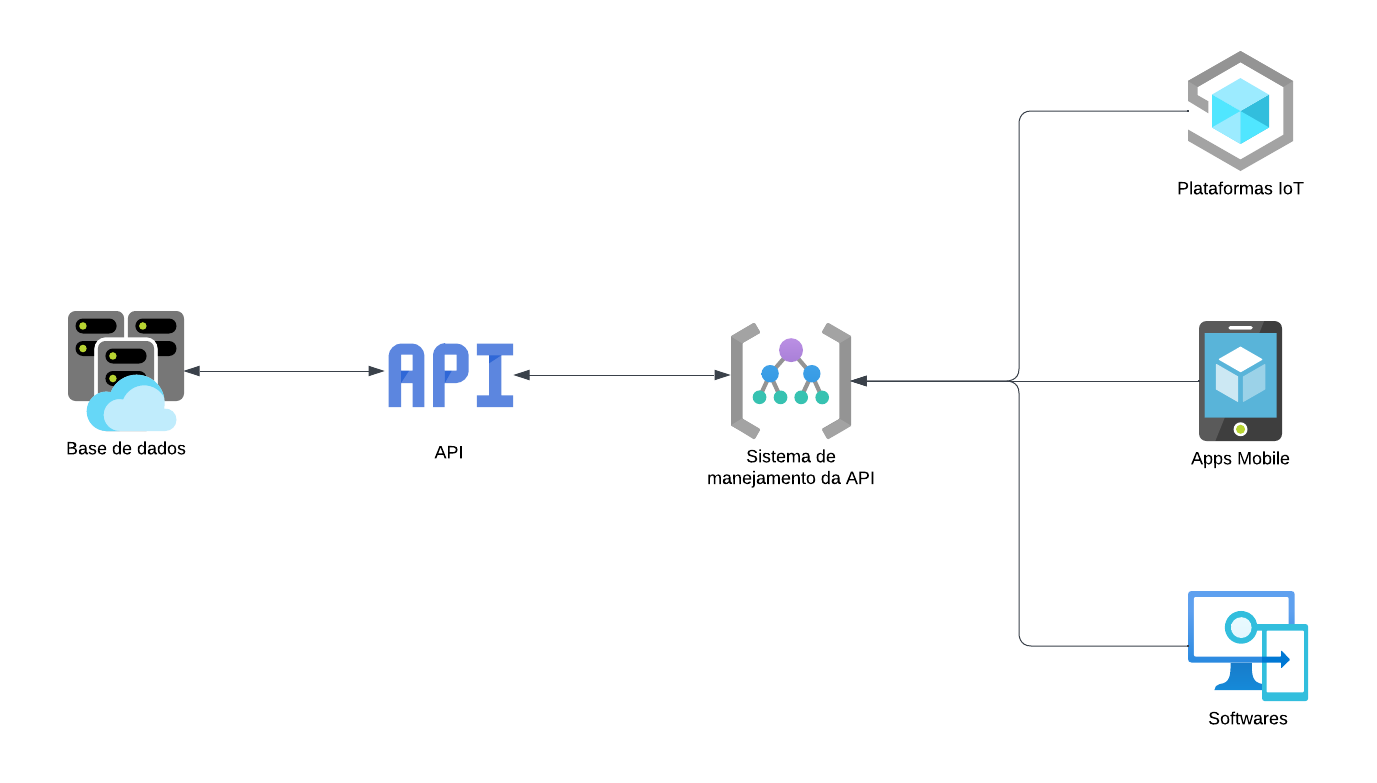
\includegraphics[scale=.57]{assets/apigenerica.png}
\caption{Representação genérica de API}
\label{apigenerica}
\end{figure}
Uma das principais vantagens das APIs é a capacidade de promover a reutilização de funcionalidades existentes em diferentes sistemas. Por meio de uma API bem projetada, os desenvolvedores podem criar novas aplicações ou integrar serviços adicionais sem precisar reinventar a roda. Isso resulta em economia de tempo e esforço, além de possibilitar a criação de soluções mais robustas e avançadas.

Além disso, as APIs também desempenham um papel crucial na criação de ecossistemas de desenvolvedores. Ao disponibilizar APIs públicas, as empresas podem estimular a criação de aplicativos de terceiros que se integram ao seu próprio sistema ou serviço. Isso não apenas amplia o alcance e a funcionalidade do sistema principal, mas também gera oportunidades de negócio e colaboração com outros desenvolvedores.

Outra área em que as APIs têm um impacto significativo é no contexto das aplicações móveis. Com o crescimento exponencial dos dispositivos móveis, as APIs desempenham um papel fundamental na comunicação entre aplicativos e serviços na nuvem. Por exemplo, aplicativos de redes sociais se comunicam com as APIs das plataformas de redes sociais para autenticação de usuários, compartilhamento de conteúdo e acesso a dados do perfil. Isso permite que os aplicativos móveis ofereçam recursos mais avançados e conectividade com outros serviços populares.

Em conclusão, as APIs desempenham um papel fundamental na integração de sistemas de software e na criação de arquiteturas distribuídas. Elas fornecem uma interface padronizada e estruturada para permitir que os sistemas se comuniquem de maneira eficiente e confiável. Com a popularização das APIs baseadas na web, como aquelas que utilizam protocolos e padrões da web, como HTTP e XML, a interoperabilidade entre sistemas se tornou mais fácil e acessível. As APIs continuam a impulsionar a inovação e a colaboração entre diferentes sistemas, abrindo caminho para o desenvolvimento de soluções mais poderosas e interoperáveis no futuro.


\section{Banco de dados}
A seção de banco de dados é um elemento crucial no desenvolvimento de uma plataforma, uma vez que é responsável por armazenar e gerenciar dados de forma eficiente. Dessa forma, a escolha do Sistema Gerenciador de Banco de Dados (SGBD) é uma etapa muito importante. Segundo \citet{Silberschatz:2010}, um SGBD consiste em uma coleção de dados inter-relacionados e um conjunto de programas para acessá-los. Essa coleção de dados, também conhecida como banco de dados, contém informações essenciais para organizações, pessoas e empresas. Desta maneira a escolha do SGBD adequado pode garantir a eficiência, segurança e escalabilidade do sistema de gerenciamento de dados, o que é fundamental para o sucesso da plataforma.

O banco de dados é projetado para armazenar informações relevantes para uma organização, pessoa ou empresa, permitindo o acesso, recuperação e manipulação eficientes desses dados. Um banco de dados consiste em tabelas, que representam entidades e seus relacionamentos, e possui um conjunto de regras e restrições que garantem a integridade e consistência dos dados. Essa abordagem centralizada e estruturada permite a organização eficiente dos dados, facilitando a consulta, atualização e análise das informações contidas no banco de dados. Com um banco de dados, é possível armazenar grandes volumes de dados de forma confiável e acessá-los de maneira rápida e eficiente, fornecendo uma base sólida para o suporte às operações e tomadas de decisão da plataforma.

A escolha do modelo de banco de dados também é um fator importante a ser considerado. Existem diferentes modelos, como o modelo relacional, o modelo de documentos, o modelo de grafos, entre outros. Cada modelo tem suas vantagens e é adequado para diferentes tipos de aplicações e cenários.

No modelo relacional, os dados são organizados em tabelas com linhas e colunas. Esse modelo é amplamente utilizado devido à sua simplicidade e capacidade de representar relacionamentos complexos entre entidades. Ele permite a realização de consultas complexas usando a linguagem SQL (Structured Query Language) e oferece recursos de integridade referencial para manter a consistência dos dados.

Por outro lado, o modelo de documentos é adequado para aplicações que trabalham com dados semiestruturados ou não estruturados. Nesse modelo, os dados são armazenados em documentos, geralmente no formato JSON ou XML, e são organizados em coleções. Esse modelo é flexível e escalável, permitindo o armazenamento de dados de diferentes estruturas e formatos.

O modelo de grafos é ideal para aplicações que envolvem relacionamentos complexos entre entidades. Nesse modelo, os dados são representados como nós (vertices) e arestas (edges) que conectam esses nós. Ele é eficiente para a consulta de relacionamentos e é usado em cenários como redes sociais, recomendações personalizadas e análise de dados em malha.

Além dos modelos de banco de dados mencionados anteriormente, também é importante considerar os bancos de dados NoSQL. Esses bancos de dados são projetados para lidar com grandes volumes de dados e cenários em que a flexibilidade e a escalabilidade são prioritárias. Eles são especialmente úteis em aplicações web e mobile, que precisam lidar com dados não estruturados, semi-estruturados ou em constante evolução. Os bancos de dados NoSQL oferecem alta disponibilidade e desempenho, permitindo a distribuição dos dados em vários servidores e a execução de operações paralelas.

Além disso, a escalabilidade do SGBD também é um fator crucial a ser considerado. À medida que a plataforma cresce e a quantidade de dados aumenta, é essencial que o SGBD possa lidar com o aumento da carga de trabalho e a demanda por desempenho. A capacidade de dimensionar horizontalmente o banco de dados, distribuindo os dados em vários servidores, pode ser uma solução para lidar com esses desafios e garantir a disponibilidade e o desempenho contínuos do sistema.

Outro aspecto importante é a interoperabilidade com outras tecnologias. Ao escolher um SGBD, é essencial considerar se ele possui integração e compatibilidade com outras ferramentas e sistemas utilizados na plataforma. Isso inclui a capacidade de se conectar a outras aplicações, serviços e APIs, além de suportar formatos de dados comuns e padrões de comunicação.

A manutenção e a otimização do banco de dados também devem ser levadas em conta. É importante escolher um SGBD que ofereça recursos de monitoramento, diagnóstico e ajuste de desempenho. Isso permite identificar e corrigir possíveis problemas, além de otimizar consultas e operações para garantir um desempenho ideal do banco de dados.

Em conclusão, o banco de dados desempenha um papel essencial na plataforma, fornecendo uma estrutura organizada e eficiente para armazenar, gerenciar e acessar dados importantes. A escolha cuidadosa do Sistema Gerenciador de Banco de Dados (SGBD) é crucial para garantir a eficiência, segurança e escalabilidade do sistema de gerenciamento de dados. Um SGBD adequado oferece recursos que permitem a manipulação eficiente dos dados, garantindo a integridade e consistência das informações. Com um banco de dados bem projetado, é possível armazenar grandes volumes de dados e realizar operações de consulta e atualização de forma confiável e eficiente. Isso fornece uma base sólida para a tomada de decisões, a execução de operações diárias e o suporte às atividades da plataforma como um todo.
\chapter{Trabalhos relacionados}
Dentro do escopo dos trabalhos realizados em colaboração com a empresa parceira, \citet{zanini2021modelagem} desenvolveu armadilhas eletrônicas que atraem e contabilizam moscas da fruta por meio de RSSF utilizando uma abordagem específica. Através dessa solução, a empresa criou duas versões de plataformas que atendem exclusivamente aos dados provenientes dessas armadilhas. No entanto, essas plataformas não são tão abrangentes e flexíveis quanto a plataforma NosConectados, que oferece perfis personalizados, métodos de autenticação e maior generalidade. Vale destacar que além disso, a plataforma NosConectados é independente da solução oferecida pela empresa, e esta pode usufruir dos benefícios da plataforma mesmo que suas soluções atuais sejam limitadas às armadilhas.

Em relação aos trabalhos correlatos na área, um estudo conduzido por \citet{Khun:2018} apresentou um aplicativo voltado para facilitar o trabalho de profissionais de agronomia, permitindo o registro de informações relacionadas ao plantio e controle de estoque. O aplicativo inclui ainda funcionalidades como cadastro de usuários e produtos pela plataforma. No entanto, diferentemente do nosso trabalho, não há nenhuma integração com redes de sensores nem disponibilização de gráficos para o usuário. Além disso, o estudo de \citet{Khun:2018} tem um enfoque mais restrito, voltado principalmente para o desenvolvimento de smartfarms. 

Em comparação, o estudo conduzido por \citet{PIERAZZOLI:2019} apresentou um sistema implementado e avaliado em escala, com acesso a sensores e atuadores próprios para a realização das tarefas necessárias, integrando-se a uma fazenda por meio da Internet das Coisas (IoT). No entanto, ao contrário do nosso trabalho proposto, esse sistema não oferece uma plataforma acessível ao usuário, que forneça dados por meio de APIs ou dashboards para apoiar a tomada de decisões. Igualmente, este estudo é exclusivamente voltado para o setor agrícola, ao passo que o nosso trabalho possui uma abordagem mais ampla e abrangente.

Dentre as soluções acadêmicas desenvolvidas, aquela que mais se assemelha à finalidade proposta neste trabalho é o mySense, descrito por \citet{mysense:2018}. O mySense possui conectividade com diversos tipos de dispositivos e oferece apoio à tomada de decisão por meio da execução de vários algoritmos de inteligência artificial. Esses algoritmos auxiliam na inferência das causas e no estabelecimento de um plano de intervenção preventiva para mitigar os efeitos de pragas e doenças nas culturas, evitando perdas significativas. A arquitetura da plataforma mySense e suas integrações podem ser visualizadas na figura \ref{mysense}. No entanto, é importante ressaltar que, apesar de ser uma plataforma elaborada, não há registros de sua implementação no mercado, o que limita uma visão detalhada de suas funções. Adicionalmente, o mySense é uma ferramenta voltada exclusivamente para o setor agropecuário, onde o monitoramento dos sensores IoT é aplicado apenas no manejo de pragas, diferenciando-se da nossa plataforma que busca monitorar dados de diferentes tipos de sensores e abranger várias áreas dentro do contexto do IoT.

\begin{figure}[htbp]
  \centering 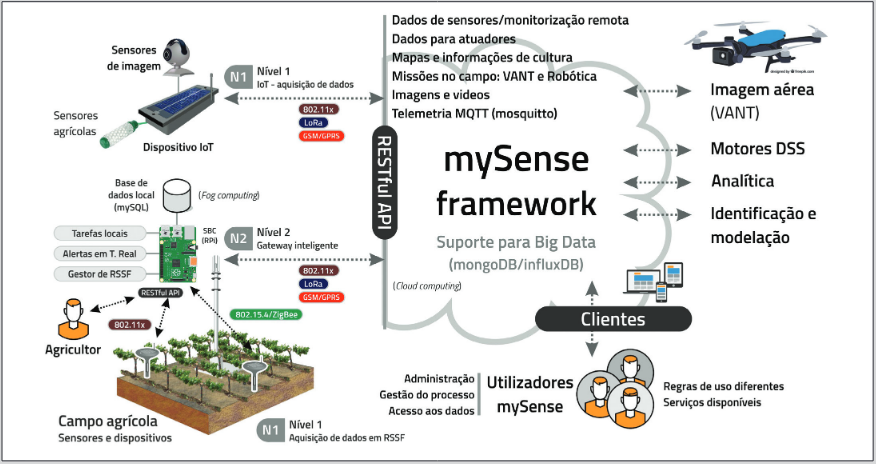
\includegraphics[scale=.45]{assets/mysense.png}
  \caption{Arquitetura da plataforma mySense}
  \UrlFont{https://www.fsantos.utad.pt/bibliografia/20AT27\_Agrobotica\_MySense\_prova3\_X.pdf}
  \label{mysense}
\end{figure}

Por se tratar de um trabalho voltado para o desenvolvimento tecnológico, em vez de uma pesquisa científica, é possível fazer comparações com alguns softwares disponíveis no mercado que possuam a mesma finalidade. Um exemplo é o Farmbox, desenvolvido para monitoramento e gestão do campo. Embora seja uma plataforma que ofereça apoio à tomada de decisão por meio de dashboards e gráficos  \cite{farmbox:2022}. Por ser uma plataforma que é exclusivamente voltada para o setor do agronegócio e é uma solução proprietária fechada, difere do nosso trabalho, uma vez que buscamos ir além do setor do agronegócio, embora ele seja um fator importante na plataforma, não será o único. Além disso, atualmente, as soluções empregadas pelo \citet{hidrosedi:2022}, em conjunto com a ALM, não apresentam integração em um sistema único. Observa-se que, em ambos os casos, são soluções proprietárias fechadas, o que dificulta a adição de funcionalidades que possam ser úteis para projetos de pesquisa que visam o desenvolvimento de novas tecnologias. Na figura \ref{farmbox}, é possível visualizar um exemplo de dashboard de monitoramento disponibilizado pela plataforma do Farmbox.

\begin{figure}[htbp]
  \centering 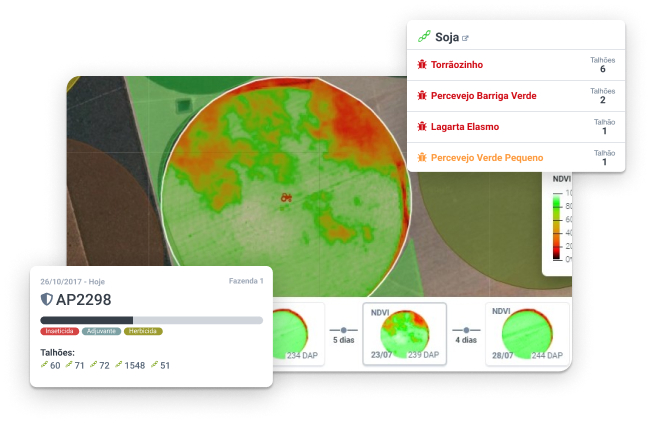
\includegraphics[scale=.7]{assets/farmbox.jpg}
  \caption{Dashboard de monitoramento do farmbox}
  \UrlFont{https://farmbox.com.br/}
  \label{farmbox}
\end{figure}
Além das soluções citadas, uma das alternativas no mercado que mais se assemelha ao trabalho proposto é a plataforma Vitau que é uma solução tecnológica voltada para o monitoramento e gestão de dispositivos IoT em diferentes setores e aplicações \cite{vitau:2023}. A plataforma oferece um conjunto de ferramentas e recursos que permitem o monitoramento em tempo real, coleta e análise de dados provenientes de sensores IoT, além de oferecer recursos de gerenciamento e controle desses dispositivos.

Uma das principais características da plataforma Vitau IoT é sua flexibilidade e adaptabilidade a diferentes contextos e setores. Ela pode ser aplicada em áreas como agronegócio, indústria, cidades inteligentes, saúde, logística, energia, entre outros. A plataforma permite o monitoramento de uma ampla gama de sensores e dispositivos, como sensores de temperatura, umidade, pressão, luminosidade, acelerômetros, entre outros \cite{vitau:2023}.

Contudo, embora compartilhe semelhanças com a plataforma Vitau IoT, como a abordagem de diversas áreas, como agronegócio e indústria, e a apresentação de dashboards interativos para o usuário, a alternativa do projeto NosConectados se destaca por sua abstração da variedade de tipos de sensores por meio de sua API. Permitindo a integração de novos sensores sem a necessidade de modificação do código-fonte, tornando-a mais flexível em relação à entrada de dados, enquanto a Vitau utiliza seus próprios sensores desenvolvidos e comercializados por eles. Além disso, a plataforma proposta neste trabalho oferece capacidade de integração com sistemas externos, possibilitando a criação de soluções personalizadas e a utilização dos dados em diferentes contextos e aplicações. Por fim, diferentemente da Vitau, a plataforma web NosConectados é uma solução aberta que pode ser utilizada para fins de pesquisa acadêmica. Na figura \ref{vitau}, é ilustrado o fluxo de funcionamento para manutenção dentro da plataforma Vitau.

\begin{figure}[htbp]
  \centering 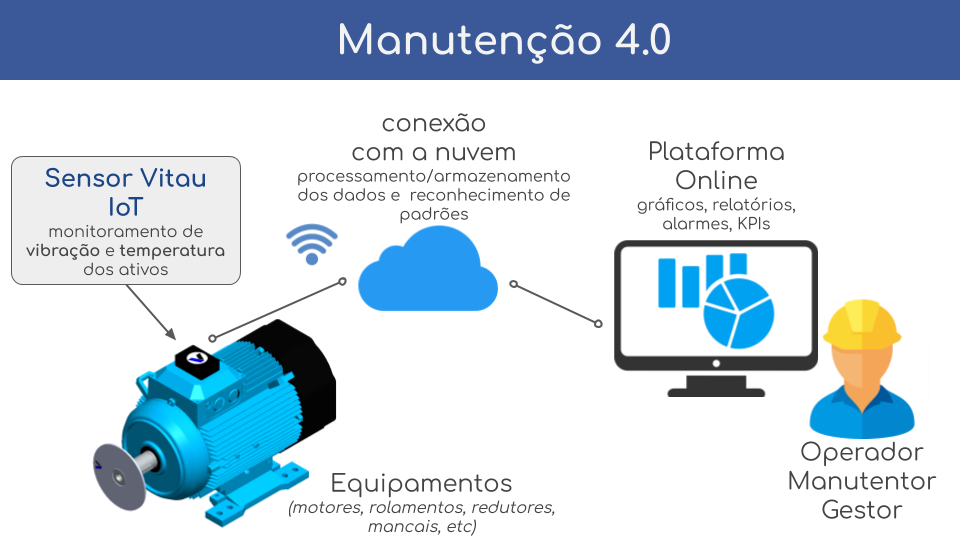
\includegraphics[scale=.4]{assets/vitau.png}
  \caption{Fluxo de manutenção dos sensores para funcionamento da plataforma Vitau}
  \UrlFont{https://vitauautomation.com/platform.html}
  \label{vitau}
\end{figure}
Portanto, os trabalhos relacionados na área apresentam diferentes abordagens e funcionalidades, mas nenhum deles oferece uma plataforma tão abrangente e integrada quanto a proposta deste trabalho. Enquanto alguns trabalhos se concentram apenas em um setor, outros possuem soluções proprietárias fechadas ou não oferecem integração com redes de sensores. Além disso, embora existam plataformas semelhantes no mercado, nenhuma delas possui a mesma amplitude de aplicação e acessibilidade ao usuário. 

Em conclusão, a proposta deste trabalho se destaca em relação aos trabalhos relacionados ao oferecer uma plataforma abrangente, integrada e flexível para o monitoramento e gestão de dispositivos IoT em diversos setores. Com sua abordagem aberta, capacidade de integração com sistemas externos e facilidade de adição de novos sensores, a plataforma NosConectados busca preencher uma lacuna no mercado, fornecendo uma solução acessível e abrangente para o monitoramento e gestão de dispositivos IoT.

\chapter{Projeto e Desenvolvimento da Plataforma Web NosConectados}
O desenvolvimento da plataforma NosConectados foi dividido em várias etapas, começando pela análise de requisitos e passando pela modelagem, desenvolvimento, testes, documentação e manutenção.

Na subseção de Análise de Requisitos, foram identificados e descritos os requisitos funcionais e não funcionais da plataforma, bem como elaborado o diagrama de casos de uso para compreender as funcionalidades e interações da aplicação.

Com base na análise de requisitos, a subseção de Modelagem detalha a elaboração dos diagramas de sequência, classes, componentes, implantação, entidade relacionamento e modelo lógico do banco de dados, que serviram de base para o desenvolvimento da plataforma.

Na subseção de Desenvolvimento, foram selecionadas cuidadosamente as ferramentas utilizadas nas diferentes camadas da aplicação, separando claramente o front-end do back-end. A abordagem do banco de dados, autenticação de usuários e sensores, camadas de segurança, controles de administração e dashboards também foram devidamente considerados e descritos nas respectivas subseções, garantindo uma implementação robusta e eficiente da aplicação.

%A subseção de Testes descreveu as etapas de teste da plataforma, %que envolveram testes unitários, testes de integração e testes de aceitação, 
%para garantir que a plataforma funcionasse corretamente e que os dados coletados fossem precisos e confiáveis. Sendo uma parte fundamental do processo de desenvolvimento da plataforma, pois garante que a mesma esteja preparada para operar de maneira adequada e atender às expectativas dos usuários.\\

A subseção de Testes descreveu as etapas realizadas para garantir o correto funcionamento da plataforma. A realização dos testes é uma etapa crucial do processo de desenvolvimento da plataforma, pois garante a sua adequação e a capacidade de atender às expectativas dos usuários. 

Na subseção de Documentação, foram criados manuais e documentação técnica para facilitar a utilização e manutenção da plataforma. Por fim, a subseção de Manutenção descreveu as estratégias de atualização de bibliotecas e frameworks da plataforma e as possíveis melhorias que foram indicadas na etapa de teste, para garantir que a plataforma estivesse sempre funcionando de forma adequada.

\section{Análise de requisitos}
\label{sec:analiserequisitos}
A análise de requisitos é uma etapa crucial do processo de desenvolvimento de software, pois é nessa fase que são identificadas e documentadas as necessidades e expectativas dos usuários finais para o sistema a ser construído. Segundo \citet{SOMMERVILLE:2011}, a análise de requisitos é um processo iterativo que envolve a coleta, a análise, a validação e a documentação de requisitos de software. 

No contexto deste trabalho, os requisitos foram definidos a partir de reuniões com o professor orientador, que atuou como representante dos usuários finais da plataforma. De acordo com \citet{PRESSMAN:2016}, em projetos em que não é possível envolver diretamente os usuários finais na análise de requisitos, é comum que um representante do cliente seja designado para atuar como um "proxy"\space entre os desenvolvedores e os usuários. Nesse caso, é fundamental que esse representante tenha conhecimento do domínio do problema e das necessidades dos usuários finais, de modo a garantir que os requisitos sejam adequadamente definidos e documentados.

Os requisitos identificados para a plataforma foram divididos em requisitos funcionais e requisitos não funcionais, conforme \citet{ghezzi:2003}. Nesta etapa, os requisitos funcionais e não funcionais foram claramente identificados e documentados, de modo a evitar ambiguidades e garantir que o sistema atenda às expectativas dos usuários finais.

Entre os requisitos funcionais identificados, destacam-se a possibilidade de monitorar múltiplas redes de sensores e a geração de gráficos para visualização dos dados. Já entre os requisitos não funcionais, foram identificados requisitos relacionados à segurança, como a necessidade de autenticação e autorização de usuários e a garantia de proteção contra ataques de injeção de SQL. Conforme enfatiza \citet{bass:2003}, a segurança é um aspecto crítico do desenvolvimento de software, e deve ser considerada desde as fases iniciais do projeto.

Para detalhar de forma mais completa os requisitos identificados, serão apresentadas duas subseções distintas que abordam os requisitos funcionais e não funcionais. Além disso, para representar graficamente o funcionamento da plataforma, serão apresentados dois diagramas distintos. O primeiro deles é o diagrama de casos de uso, que descreve as principais funcionalidades do sistema e como os atores interagem com elas. O segundo diagrama é o de sequência, que ilustra como as diferentes funcionalidades são executadas ao longo do tempo e como interagem entre si.

\subsection{Requisitos funcionais}
De acordo com \citet{PRESSMAN:2016}, os requisitos funcionais são as descrições das funções, serviços ou atividades que o sistema deve ser capaz de realizar. Eles definem o que o sistema deve fazer, sem especificar como isso deve ser feito. O autor também destaca a importância da priorização e organização desses requisitos em ordem de importância. Essa abordagem permite que os recursos limitados do projeto sejam alocados de forma eficiente e que as funcionalidades mais importantes sejam entregues primeiro, garantindo assim que o sistema atenda às necessidades do usuário.

\citet{SOMMERVILLE:2011} por sua vez, sugere o uso de técnicas como casos de uso, histórias de usuário e especificações de requisitos. O autor ressalta a importância de garantir que esses documentos sejam claros, concisos e facilmente compreensíveis, para que possam ser compartilhados com a equipe de desenvolvimento e outras partes interessadas.

Além dos requisitos funcionais já citados anteriormente, existem outros que são essenciais para garantir o pleno funcionamento da plataforma. Dentre eles, podemos destacar a capacidade de integração com outros sistemas e a possibilidade de personalização das funcionalidades de acordo com as necessidades específicas dos usuários.

Além disso, a capacidade de processamento de dados em tempo real é uma funcionalidade importante para permitir que os usuários obtenham informações atualizadas sobre o status de seus dispositivos e sensores, o que possibilita uma tomada de decisão mais rápida e eficiente. Com isso, é possível realizar ajustes e correções antes que problemas mais graves ocorram. A possibilidade de atribuir um sensor a diversos usuários também é uma funcionalidade relevante, o que garante uma melhor distribuição e gerenciamento de responsabilidades entre os envolvidos.

Outro requisito funcional importante é a possibilidade da criação de diferentes perfis de usuários, com diferentes níveis de acesso às informações. Por exemplo, administradores do sensor podem ter acesso a informações mais detalhadas, enquanto os patrocinadores serão responsáveis pela manutenção dos sensores e teriam acesso apenas às informações técnicas e operacionais, e por fim os visualizadores são úteis para sensores privados. Isso permitirá que os usuários acessem apenas as informações relevantes para suas atividades, garantindo a privacidade e segurança das informações.

Por conseguinte, seguindo a visão de \citet{PRESSMAN:2016}, os requisitos funcionais identificados para a plataforma foram organizados na seguinte ordem de importância:
\begin{enumerate}
    \item Criação de diferentes perfis de usuários
    \item Monitoramento de múltiplas redes de sensores através da abstração da API
    \item Geração de gráficos para visualização dos dados (dashboards)
    \item Possibilidade de atribuir um sensor a diversos usuários
    \item Personalização das funcionalidades de acordo com as necessidades específicas dos usuários
    \item Processamento em tempo real
    \item Capacidade de integração com outros sistemas
\end{enumerate}

Dessa forma, podemos concluir que a priorização criteriosa desses requisitos, considerando a importância de cada funcionalidade, possibilitará uma alocação eficiente dos recursos disponíveis, sendo sua definição clara e organizada um elemento fundamental para o sucesso do projeto de desenvolvimento da plataforma. Com todos esses requisitos funcionais devidamente definidos e implementados, a plataforma estará pronta para atender plenamente às necessidades dos usuários, proporcionando uma experiência eficiente e eficaz.

\subsection{Requisitos não-funcionais}
Os requisitos não-funcionais da plataforma NosConectados são cuidadosamente definidos, seguindo a abordagem proposta por \citet{book:chung:2000}, com o objetivo de garantir a qualidade e eficiência do software. Dentre esses requisitos, o desempenho é prioritário, assegurando que a plataforma seja projetada para realizar requisições ao servidor de forma eficiente, com tempos de resposta adequados. A usabilidade é uma preocupação constante, com a busca por uma interface intuitiva e amigável que proporcione uma experiência fácil e agradável ao usuário final. A segurança dos dados é outro requisito estritamente considerado, com restrição de acesso e proteção de informações sensíveis para garantir a confidencialidade e integridade dos dados. A escalabilidade é um aspecto importante, permitindo que a plataforma suporte múltiplos usuários simultaneamente sem perda de desempenho, visando atender às demandas crescentes do sistema. Além disso, a manutenibilidade é buscada por meio de um código limpo e bem documentado, possibilitando uma fácil manutenção e atualização da plataforma.

Para garantir que os requisitos não funcionais identificados sejam atendidos de forma efetiva, eles serão abordados em ordem de importância, seguindo a mesma abordagem utilizada para os requisitos funcionais.

\begin{enumerate}
\item Implementação de medidas de segurança robustas, incluindo técnicas de encriptação de informações sensíveis, para garantir a proteção adequada dos dados dos usuários.
\item Desempenho da plataforma e otimização das requisições ao servidor para garantir uma resposta rápida e eficiente.
\item Exploração dos conceitos de UI/UX visando aprimorar a usabilidade da plataforma e proporcionar uma experiência positiva aos usuários.
\item Promoção da interoperabilidade da plataforma, permitindo sua integração com outros sistemas e soluções, para facilitar a troca de informações e a colaboração em diferentes ambientes.
\item Planejamento de escalabilidade, visando suportar um grande número de usuários simultâneos sem perda de desempenho ou qualidade do serviço.
\item Implementação de práticas de manutenibilidade, como modularização do código e utilização de boas práticas de programação, para facilitar a gestão, atualização e correção de problemas na plataforma ao longo do tempo.
\end{enumerate}

 Além disso, de acordo com \citet{PRESSMAN:2016}, o teste de requisitos não-funcionais é tão importante quanto o teste de requisitos funcionais, e ambos devem ser abordados em um plano abrangente de testes. Caso contrário, o software pode apresentar problemas de desempenho, segurança ou usabilidade, afetando diretamente a satisfação do usuário e a qualidade do software como um todo. Por isso, os requisitos definidos nesta seção também servirão para auxiliar na etapa de testes da plataforma.

Dessa forma, concluímos que a abordagem cuidadosa na definição e consideração dos requisitos não-funcionais na plataforma NosConectados desde as fases iniciais do desenvolvimento evidencia o compromisso com a qualidade do software. Os requisitos não-funcionais, como desempenho, usabilidade, segurança, confiabilidade, interoperabilidade, escalabilidade e manutenibilidade, foram claramente definidos e servirão como base para os testes descritos na seção \ref{sec:testes}. A inclusão desses requisitos e sua devida avaliação garantirão que a plataforma esteja em conformidade com as expectativas dos usuários.
\subsection{Diagrama de casos de uso}
Conforme \citet{BOOCH:2007}, o objetivo de uma diagramação por meio de casos de uso é justamente fornecer uma representação gráfica dos principais requisitos funcionais de um sistema. Essa técnica descreve a interação entre atores (usuários ou outros sistemas) e o sistema em si, apresentando os principais cenários de uso do sistema de forma clara e objetiva.

O diagrama de casos de uso é composto por atores, casos de uso e suas relações. Os atores são representados por ícones e os casos de uso por elipses. As relações entre atores e casos de uso são representadas por linhas, que podem ser de associação, de generalização ou de inclusão.

Na nossa plataforma, escolhemos utilizar os casos de uso como uma abordagem para representar o sistema. Na Figura \ref{casosuso}, é possível observar a diagramação do sistema em formato de casos de uso, que apresenta seis atores relacionados à plataforma e ao gerenciamento de sensores.

\begin{figure}[htbp]
  \centering 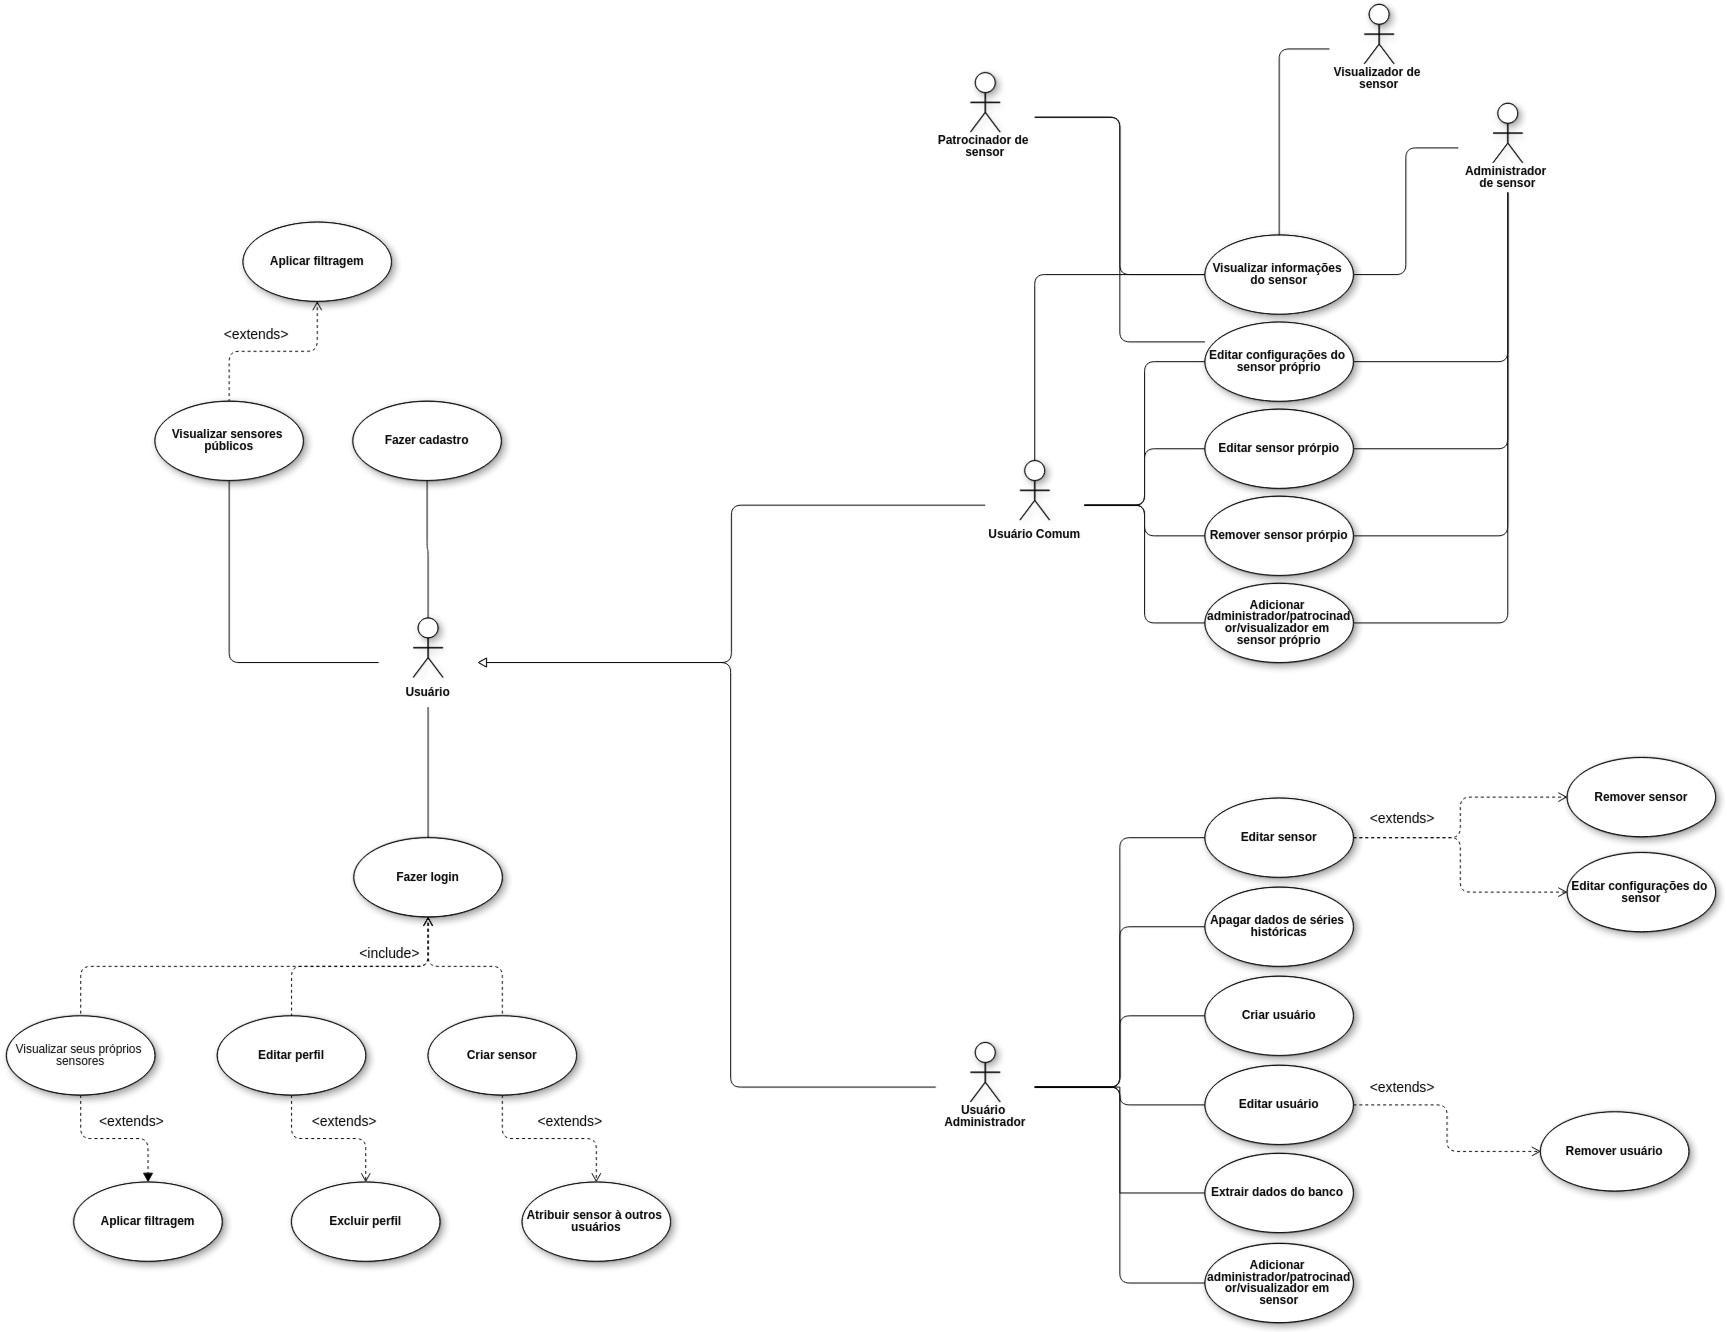
\includegraphics[scale=.22]{assets/casosdeuso.png}
  \caption{Diagrama de casos de uso}
  \label{casosuso}
\end{figure}

O primeiro ator é o Usuário, que pode se cadastrar na plataforma, fazer login e visualizar os sensores públicos. Ao visualizar os sensores públicos, ele pode utilizar uma filtragem, caso deseje. Ao fazer login, o Usuário pode visualizar os seus próprios sensores, aplicar filtragens, editar o seu perfil e remover o seu perfil, se desejar. Além disso, o Usuário também pode criar um sensor e atribuí-lo a outro usuário, se desejar.

O segundo ator é o Usuário Administrador, que possui acesso total à plataforma e pode criar, editar e remover sensores e usuários. Adicionalmente, tem a capacidade de adicionar outros Usuários como administradores, patrocinadores ou visualizadores em um sensor, editar as configurações do sensor e exportar os dados do banco de dados. Além disso, o Usuário Administrador tem o poder de excluir dados históricos gerados pelos sensores, proporcionando maior controle sobre as informações armazenadas. O Usuário Administrador herda as permissões do Usuário e possui privilégios adicionais para gerenciar a plataforma.


O terceiro ator é o Usuário Comum, que pode criar sensores, editar seus próprios sensores, remover seus próprios sensores, adicionar administradores, patrocinadores ou visualizadores em seus próprios sensores e editar as configurações dos seus sensores. O Usuário Comum também herda as permissões do Usuário, mas possui restrições adicionais em comparação ao Usuário Administrador.

Os outros três atores - Administrador de Sensor, Patrocinador de Sensor e Visualizador de Sensor - são criados à medida que um Usuário, seja ele Usuário Administrador ou Usuário Comum, cria um sensor. Esses atores herdam as permissões e informações do Usuário Comum ou Usuário Administrador, dependendo de quem criou o sensor.

O Administrador de Sensor pode editar o sensor, adicionar administradores, patrocinadores ou visualizadores no sensor e editar as configurações do sensor. Já o Patrocinador de Sensor pode editar apenas as informações do sensor. O Visualizador de Sensor, por sua vez, possui apenas permissão para visualizar as informações do sensor.

Vale ressaltar também que os atores Administrador de Sensor, Patrocinador de Sensor e Visualizador de Sensor não são herdados diretamente do Usuário Comum, mas são criados como papéis específicos após a criação de um sensor por parte do Usuário Comum ou do Usuário Administrador.

O Usuário Comum e o Usuário Administrador têm a capacidade de criar um sensor, o que resulta na criação do Administrador de Sensor associado a esse sensor. Em seguida, o Administrador de Sensor tem a capacidade de adicionar Patrocinador de Sensor e Visualizador de Sensor específicos para esse sensor. Esses atores (Administrador de Sensor, Patrocinador de Sensor e Visualizador de Sensor) têm papéis e permissões específicos relacionados ao sensor em questão, e não são uma herança direta do Usuário Comum ou do Usuário Administrador. Eles são criados como atores independentes após a criação do sensor e têm suas próprias capacidades e responsabilidades dentro do contexto do sistema.

Desta maneira, utilizando o diagrama de casos de uso como método de análise e modelagem, foi possível obter uma visão mais clara e organizada das principais funcionalidades do sistema em questão. A representação gráfica dos atores e suas interações com o sistema permitiu uma compreensão mais abrangente dos requisitos funcionais necessários para o desenvolvimento da plataforma. Ademais, a ferramenta possibilitou a identificação de possíveis lacunas ou inconsistências nas funcionalidades propostas, contribuindo para a melhoria do planejamento e implementação do sistema. Com o uso do diagrama de casos de uso, espera-se que a etapa de desenvolvimento da plataforma seja mais eficiente e eficaz.

%\subsection{Diagrama de estados}
%Segundo \citet{HAREL:1987}, o principal objetivo de um diagrama de estados é descrever o comportamento dinâmico de um objeto, apresentando a evolução de seu estado em resposta a estímulos internos ou externos. Com isso, podemos identificar potenciais problemas de design, simplificar a implementação do sistema e auxiliar no teste e na validação da plataforma.\\

%Um diagrama de estados é composto por um conjunto de estados, transições entre esses estados e atividades que ocorrem durante essas transições. Os estados representam as condições que um objeto pode assumir em um determinado momento, enquanto as transições representam os eventos que fazem o objeto mudar de um estado para outro \cite{HAREL:1987}. As atividades representam as ações que ocorrem durante uma transição, tais como cálculos, verificação de condições e atualização de variáveis \cite{LARMAN:2011}.\\

%Em resumo, um diagrama de estados é utilizado para representar o comportamento dinâmico de um sistema. Ele pode ser utilizado para especificar as transições de estado, eventos, condições e ações que ocorrem durante o processamento, bem como para auxiliar na implementação do sistema e verificar a consistência e a corretude da especificação.

\section{Modelagem}
\label{sec:modelagem}
A modelagem, em termos de software, é uma técnica utilizada na engenharia de software para representar as características, funcionalidades e comportamentos de um sistema de software em desenvolvimento. De acordo com \citet{PRESSMAN:2016}, a modelagem é uma das principais atividades da fase de análise e projeção de um projeto de software, sendo utilizada para definir e especificar os requisitos do sistema e para planejar sua implementação.

Essa etapa é realizada com base na análise de requisitos descrita na seção \ref{sec:analiserequisitos} e envolve a criação de diferentes tipos de modelos que servirão como base para o desenvolvimento da plataforma. Esses modelos incluem o Diagrama de Classes, que é utilizado para especificar as classes do sistema, seguindo uma abordagem orientada a objetos. Ele representa a estrutura do sistema e as relações entre as classes.

Além disso, com base no Diagrama de Casos de Uso elaborado na etapa de análise de requisitos, foi desenvolvido um Diagrama de Sequência que abordou os principais casos de uso identificados, tais como login do usuário, cadastro, visualização e criação de sensores. Esse diagrama permitiu uma melhor compreensão das interações e fluxos de informação envolvidos nos processos da plataforma.

Adicionalmente, utilizamos o Diagrama de Componentes, com o intuito de representar o sistema físico da plataforma, incluindo as páginas que serão desenvolvidas na parte de front-end, as funcionalidades do servidor, os componentes do back-end e do banco de dados. Como a plataforma é web e utiliza o modelo cliente-servidor, o diagrama de componentes é útil para visualizar a arquitetura do sistema.

Também utilizamos o Diagrama de Implantação, que é usado para descrever como a plataforma será implementada e implantada em um ambiente de produção. Ele representa os componentes do sistema e suas interações em um ambiente de implantação real.

Por fim, realizamos a Modelagem de Dados, que inclui o Diagrama Entidade-Relacionamento (DER) e o Modelo Lógico do Banco de Dados. Esses modelos são utilizados para representar a estrutura e as relações dos dados da plataforma, auxiliando no desenvolvimento do banco de dados.

Neste contexto, adotamos o Processo Unificado, que é um processo iterativo e incremental, no qual cada iteração resulta em uma nova versão do sistema com funcionalidades adicionais ou melhoradas em comparação com a versão anterior. Utilizamos os artefatos UML para descrever os diagramas dentro do paradigma de orientação a objetos, o que permite uma representação clara e detalhada da plataforma, incluindo suas funcionalidades, estrutura de dados e interações do usuário.

\subsection{Diagrama de classes}
Um diagrama de classes é uma ferramenta utilizada na modelagem de sistemas orientados a objetos, que permite representar a estrutura estática do sistema em termos de classes, seus atributos, métodos e relações entre elas. Segundo \citet{BOOCH:2007}, um diagrama de classes é composto por caixas retangulares que representam as classes e suas características, e linhas que representam as associações entre elas. Cada classe pode ter atributos, que são as características dos objetos dessa classe, e métodos, que são as operações que podem ser realizadas com os objetos.

Além disso, os diagramas de classes também permitem que sejam identificadas as generalizações e especializações entre as classes, ou seja, as hierarquias de herança presentes no sistema. Essa representação permite uma melhor compreensão da estrutura do sistema, facilitando a sua manutenção e evolução \citet{BOOCH:2007}. Por meio dos diagramas de classes, é possível visualizar a estrutura do sistema de forma clara e objetiva, possibilitando que a equipe de desenvolvimento trabalhe de maneira mais organizada e eficiente.

O diagrama de classes da plataforma é composto por 11 classes principais, cada uma com um propósito específico, como pode ser observado na figura \ref{diagramaclasses}. Essa representação visual permite identificar claramente as classes que compõem o sistema e suas interações.

\begin{figure}[htbp]
  \centering 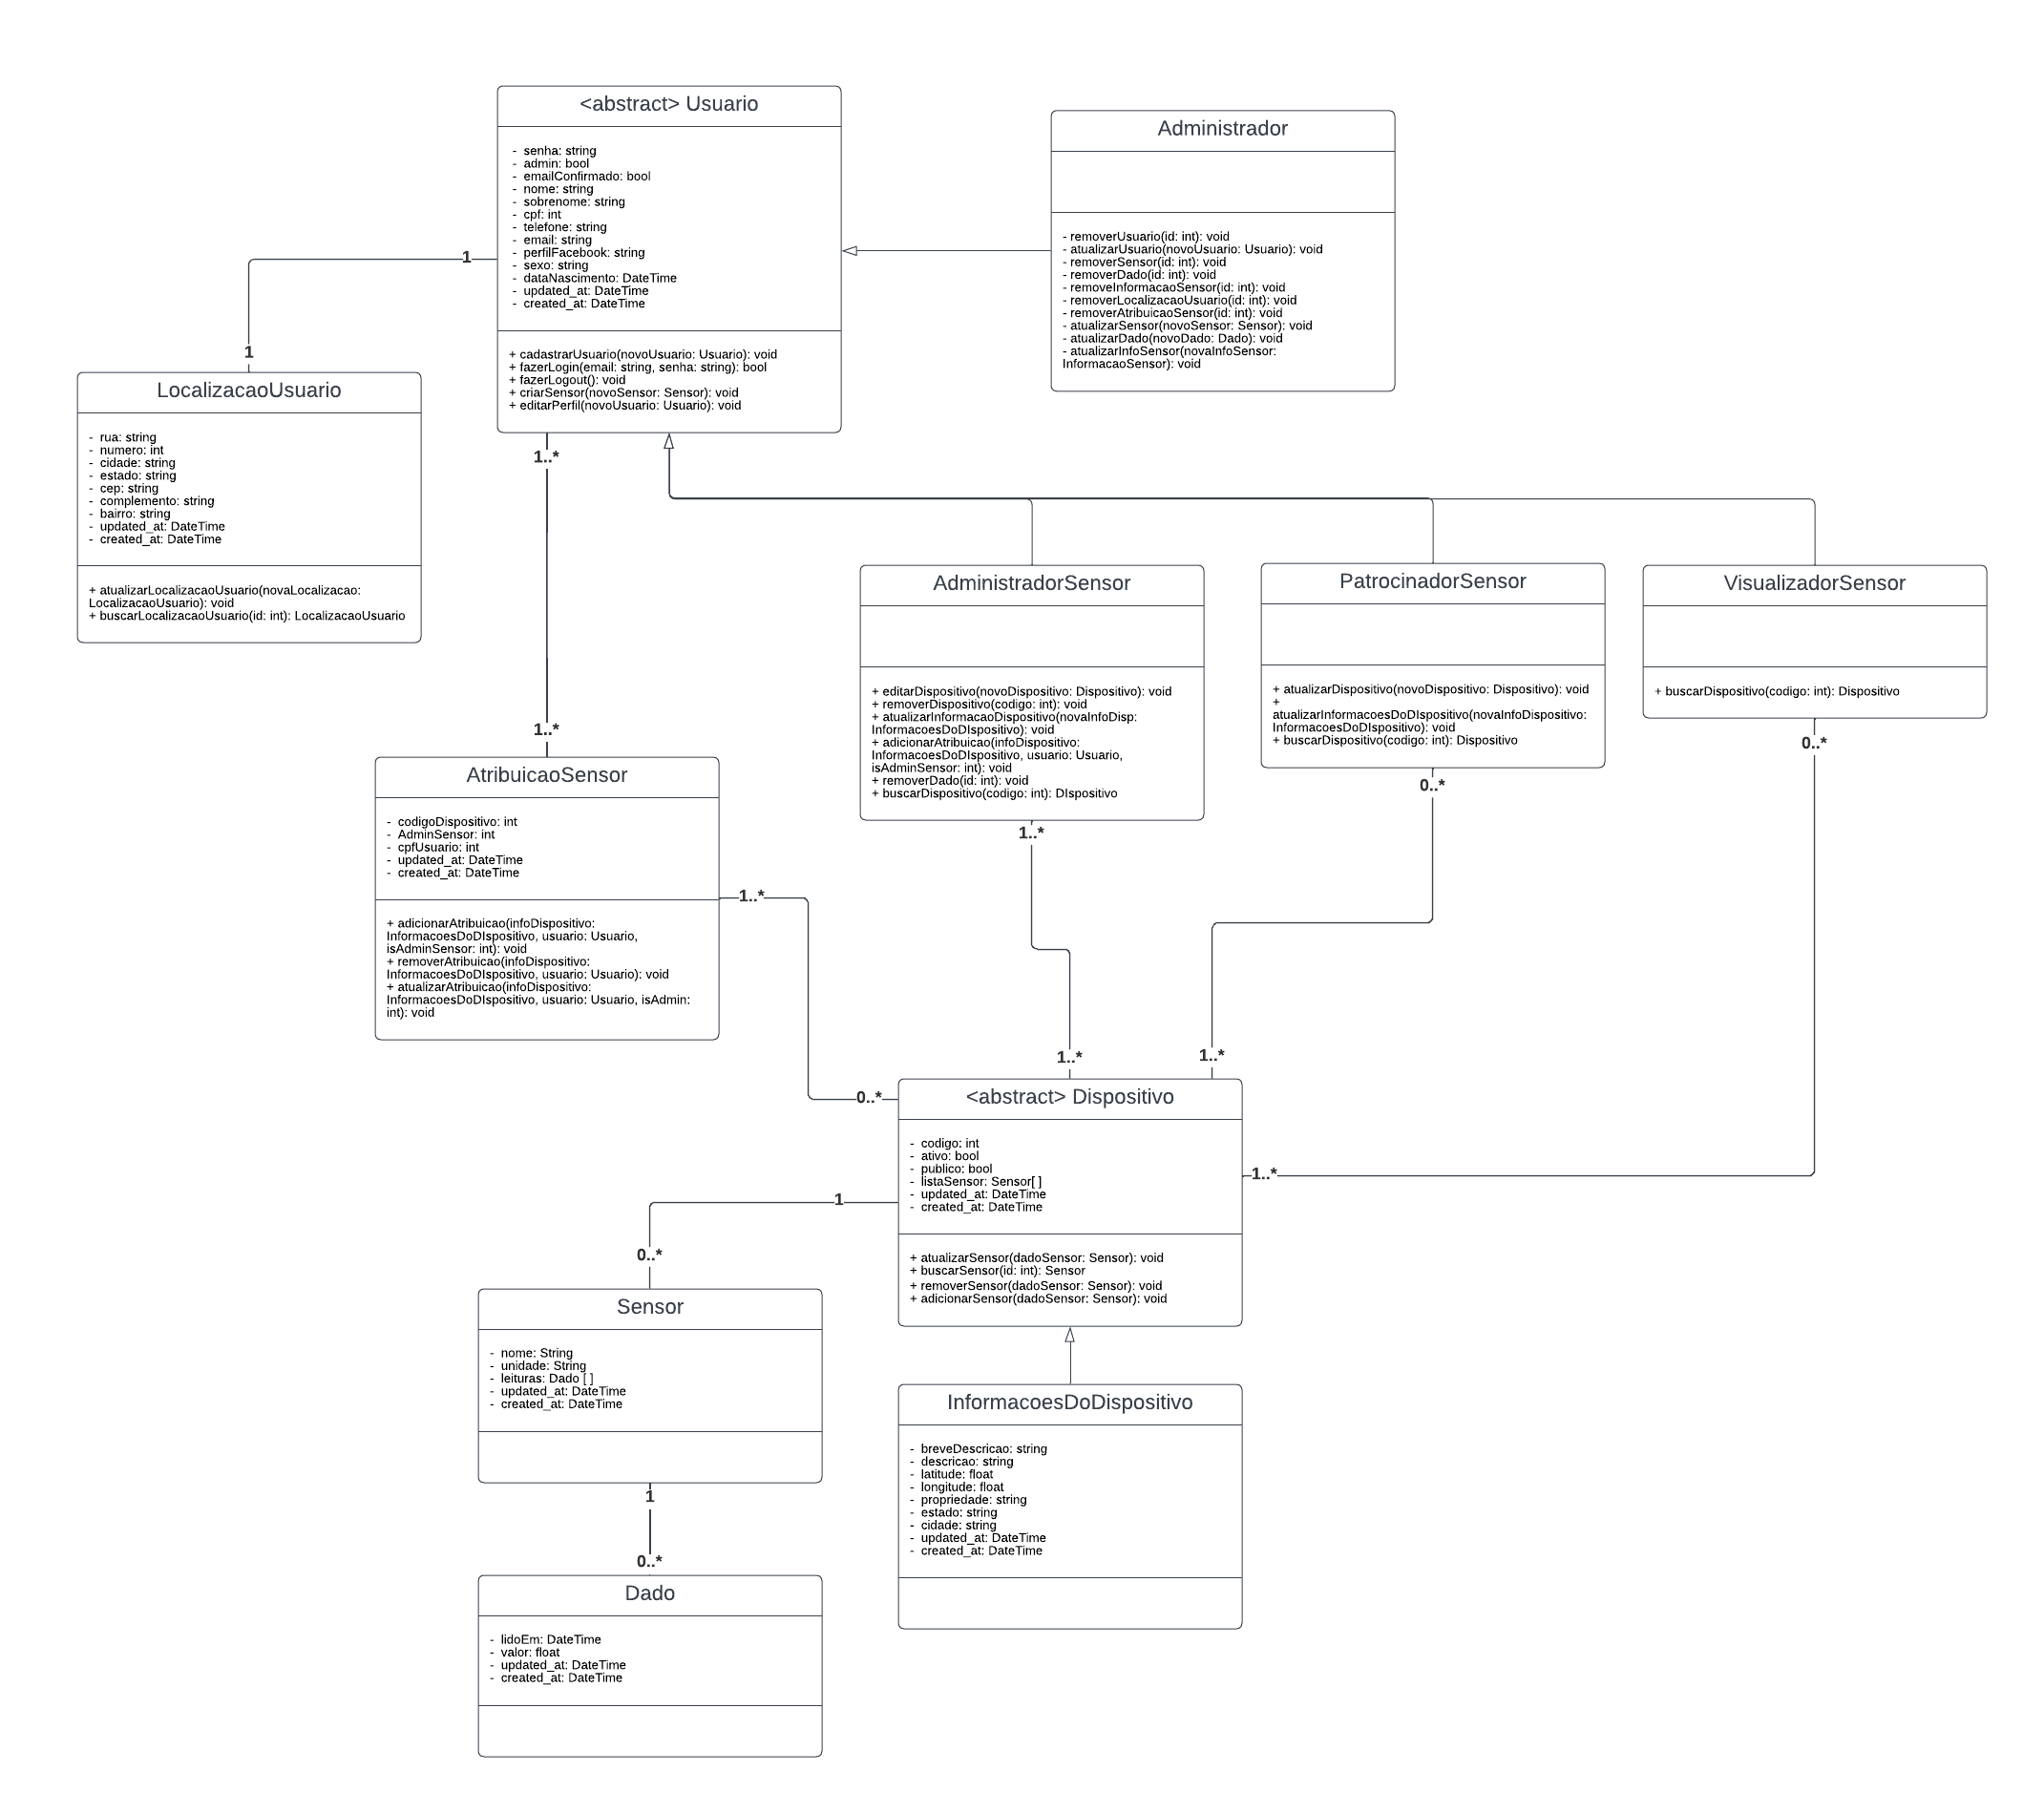
\includegraphics[scale=.5]{assets/diagramaclasses.png}
  \caption{Diagrama de classes}
  \label{diagramaclasses}
\end{figure}
\newpage


A classe de Usuario é a classe base, da qual herdam outras classes como Administrador, AdministradorSensor, PatrocinadorSensor e VisualizadorSensor, que possuem funções específicas relacionadas à administração e visualização de sensores na plataforma. Além disso, o diagrama de classes também inclui a classe de LocalizacaoUsuario, que possui uma relação de dependência com a classe Usuario, indicando que a localização do usuário é necessária para o funcionamento do sistema. Outra classe importante é a AtribuicaoSensor, responsável por atribuir sensores a usuários específicos, garantindo o correto funcionamento da plataforma. Além dessas classes, o diagrama também inclui a classe Sensor, que é a base para a classe Dado, que depende diretamente da classe Sensor para armazenar dados históricos relacionados aos sensores na plataforma.

Essa hierarquia de classes permite uma organização estruturada do sistema, possibilitando a correta representação das entidades e suas interações, fornecendo uma visão mais clara e abstrata das classes e suas relações, auxiliando no desenvolvimento, manutenção e compreensão do sistema como um todo.

Em resumo, o diagrama de classes é uma ferramenta fundamental na modelagem de sistemas orientados a objetos. Ele permite representar de forma clara e objetiva a estrutura estática do sistema, por meio de elementos como classes, atributos, métodos e relacionamentos. Através dessa representação visual, é possível visualizar de forma organizada e eficiente a composição do sistema e suas interações. Essa compreensão facilita a manutenção e evolução do sistema, tornando o diagrama de classes uma ferramenta indispensável na engenharia de software.


\subsection{Diagrama de sequência}
O principal objeto de um diagrama de sequência é representar a interação entre objetos em um sistema, descrevendo a sequência de mensagens trocadas entre eles. Na visão de \citet{PRESSMAN:2016}, o diagrama de sequência é uma técnica de modelagem comportamental que permite representar a interação entre objetos em um sistema, mostrando a ordem e o tempo em que as mensagens são trocadas. Para \citet{SOMMERVILLE:2011}, o diagrama de sequência é uma das principais ferramentas de modelagem utilizadas para descrever o comportamento dinâmico de um sistema, permitindo a análise e a verificação da lógica de interação entre os objetos. \citet{LARMAN:2011}, por sua vez, afirma que ele é utilizado para "mostrar a interação entre objetos em um contexto específico, focando na ordem temporal dos eventos".

Durante a seleção da modelagem dos diagramas de sequência para as funcionalidades da plataforma, optamos por representar os principais casos de uso, como o login, o cadastro de usuários, a criação de sensores e a visualização de sensores. Em todos os diagramas de sequência, o ator é representado pelo usuário, enquanto os objetos representados são o navegador, onde o usuário interage e insere os dados; a API, responsável por facilitar a comunicação entre o navegador e o servidor de banco de dados para validar os dados e retornar mensagens ou inserir dados no banco; e o próprio banco de dados, responsável por armazenar as informações da plataforma. Na Figura \ref{sdlogin}, é apresentado o diagrama de sequência para o caso de uso de login do usuário.

\begin{figure}[htbp]
  \centering 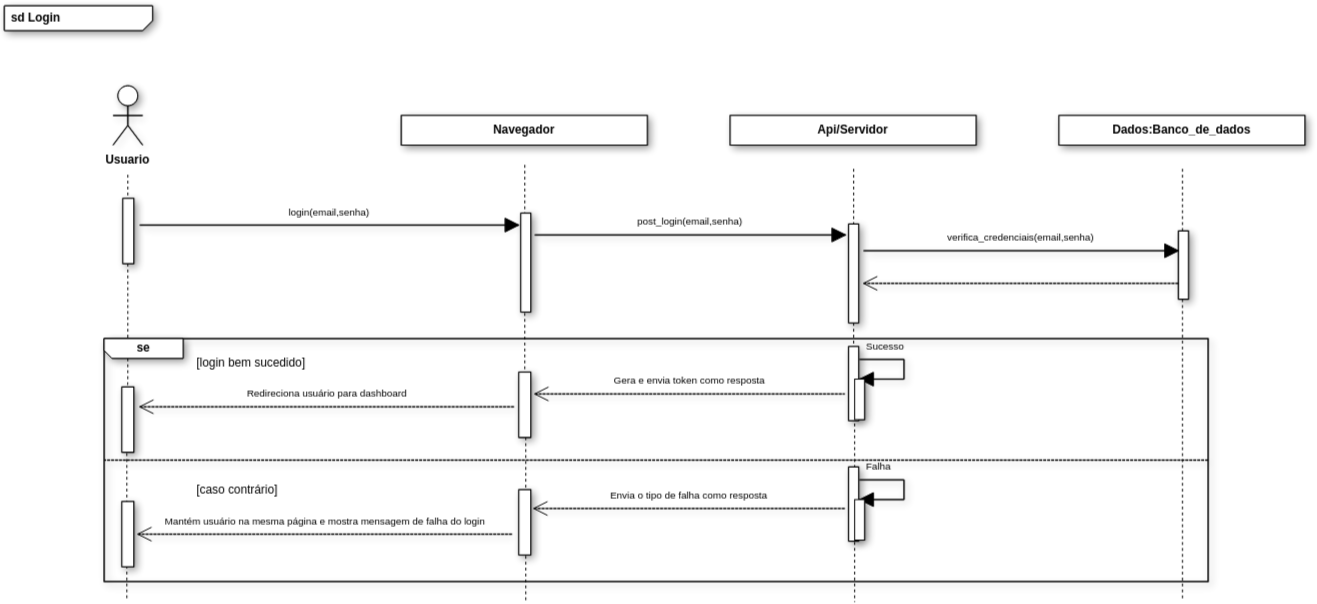
\includegraphics[scale=.3]{assets/sdlogin.png}
  \caption{Diagrama de sequência para o caso de uso de login do usuário}
  \label{sdlogin}
\end{figure}
No diagrama de sequência em questão, é possível observar o seguinte comportamento do usuário: ele insere seu e-mail e senha em um formulário no navegador. Em seguida, o navegador envia esses dados usando o método POST do protocolo HTTP para a API. A API, por sua vez, busca esses dados no banco de dados e, se as credenciais do usuário forem autenticadas, gera um token e o envia de volta para o navegador. O navegador recebe o token e redireciona o usuário para a página de dashboard. No entanto, se as credenciais estiverem incorretas, o navegador mantém o usuário na mesma página e exibe uma mensagem informando que os dados inseridos estão incorretos.

Na plataforma, também é relevante incluir um diagrama de sequência para o caso de uso de criação de sensores, onde os usuários podem inserir informações personalizadas para um sensor específico, que será posteriormente associado a um hardware instalado em campo, e também permitir a atribuição desse sensor a outros usuários. Dessa forma, é possível ter uma representação clara do fluxo de interação entre os objetos envolvidos. O diagrama de sequência para esse caso de uso pode ser visualizado na Figura \ref{sdcriar_sensor}.

\begin{figure}[htbp]
  \centering 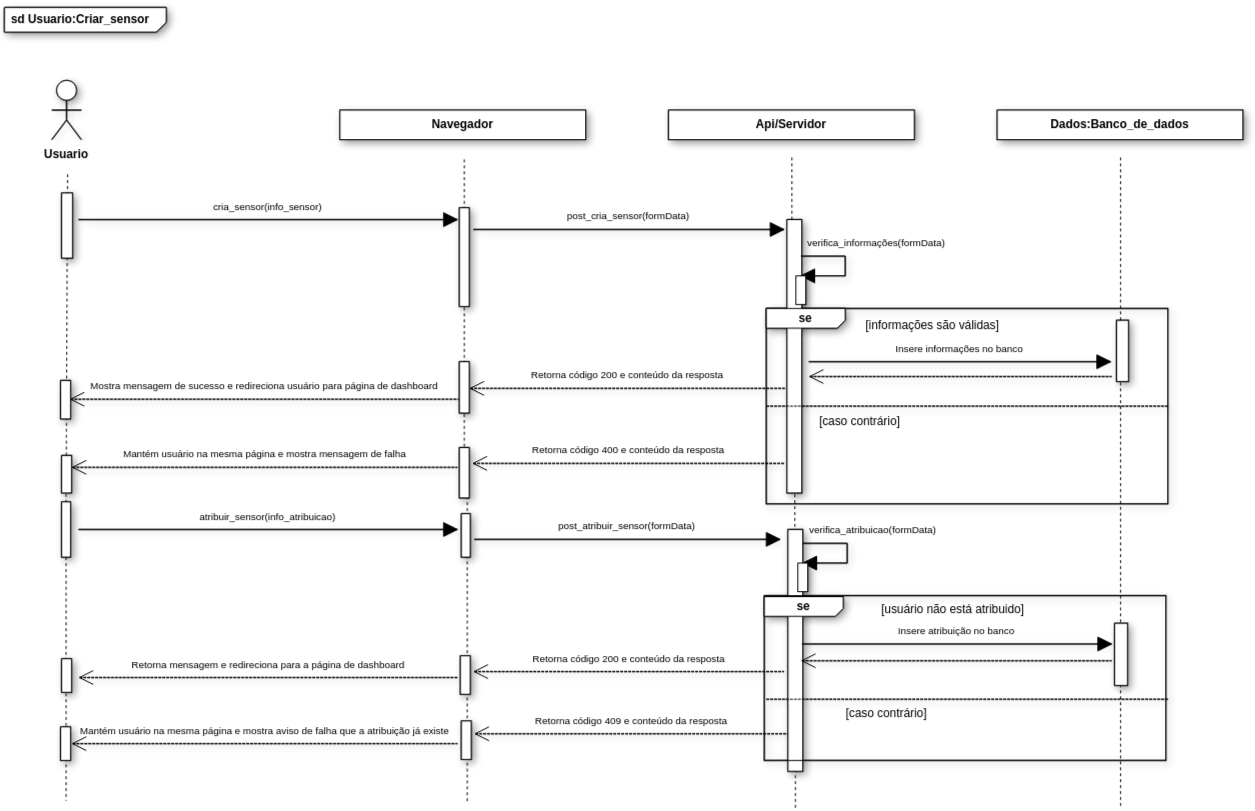
\includegraphics[scale=.3]{assets/sdcriar_sensor.png}
  \caption{Diagrama de sequência para o caso de uso de criar um sensor}
  \label{sdcriar_sensor}
\end{figure}
\newpage

Inicialmente, o usuário preenche as informações do sensor desejado em um formulário no navegador. Em seguida, o formulário envia esses dados usando o método POST para a API. A API verifica as informações recebidas e, se forem válidas, os dados são inseridos no banco de dados e a API retorna um código de resposta HTTP 200, indicando que a requisição foi processada com sucesso no servidor. O conteúdo do corpo da resposta é enviado de volta para o navegador, que exibe a mensagem ao usuário e o redireciona para a página de dashboard.

No entanto, se as informações fornecidas pelo usuário para a criação do sensor forem inválidas, a API retorna um código HTTP 400, juntamente com uma mensagem explicativa no corpo da resposta. O navegador exibe essa mensagem ao usuário e o mantém na mesma página.

Posteriormente, o usuário pode preencher os campos para atribuir o sensor a outros usuários no navegador. O navegador envia esses dados para a API usando o método POST. A API verifica as informações de atribuição e, se o usuário já estiver atribuído ao sensor ou estiver tentando atribuí-lo a si mesmo por engano, a API retorna um código de resposta HTTP 409, juntamente com uma mensagem explicativa no corpo da resposta. O navegador exibe essa mensagem ao usuário e o mantém na mesma página.

Caso o usuário não esteja atribuído ao sensor e as informações de atribuição sejam válidas, os dados são inseridos no banco de dados e a API retorna um código de resposta HTTP 200. O navegador exibe uma mensagem de sucesso ao usuário e o redireciona para a página de dashboard.

Outro diagrama de sequência fundamental em nosso sistema é o de cadastro de usuários, que representa o fluxo de interações do usuário com a plataforma. Na Figura \ref{sdcadastro}, podemos observar como esse diagrama é representado e como descreve o comportamento do sistema em relação ao cadastro de novos usuários.

\begin{figure}[htbp]
  \centering 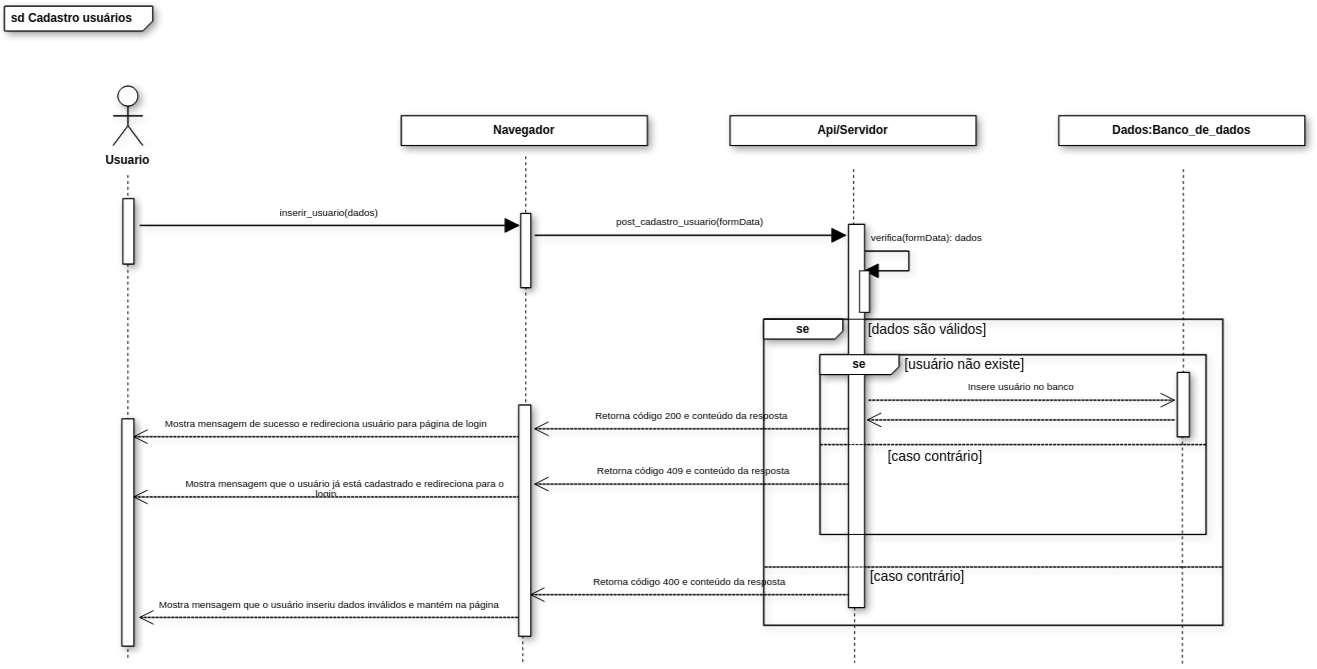
\includegraphics[scale=.3]{assets/sdcadastro.png}
  \caption{Diagrama de sequência para o caso de uso de cadastro do usuário}
  \label{sdcadastro}
\end{figure}

É perceptível que o usuário preencheria seus dados em um formulário no navegador, e em seguida, o navegador enviaria esses dados através de um método POST para a API. A API, por sua vez, verificaria a validade desses dados e, caso sejam válidos, verificaria se o usuário já existe na plataforma. Se o usuário não existir, as informações seriam inseridas no banco de dados e a API retornaria o código de resposta 200 para o navegador, que exibiria uma mensagem de sucesso ao usuário e o redirecionaria para a página de login. Porém, se o usuário já existir, a API retornaria o código de resposta 409 para o navegador, juntamente com uma mensagem no corpo da resposta, informando ao usuário que ele já está cadastrado, e o redirecionaria para a página de login. Por outro lado, se as informações fornecidas pelo usuário forem inválidas, ou seja, se houver dados incorretos no formulário de cadastro, a API retornaria o código de resposta 400, juntamente com uma mensagem no corpo da resposta. Nesse caso, o navegador exibiria uma mensagem ao usuário informando que os dados estão incorretos e o manteria na mesma página, permitindo que ele refaça o cadastro corretamente.

\begin{figure}[htbp]
  \centering 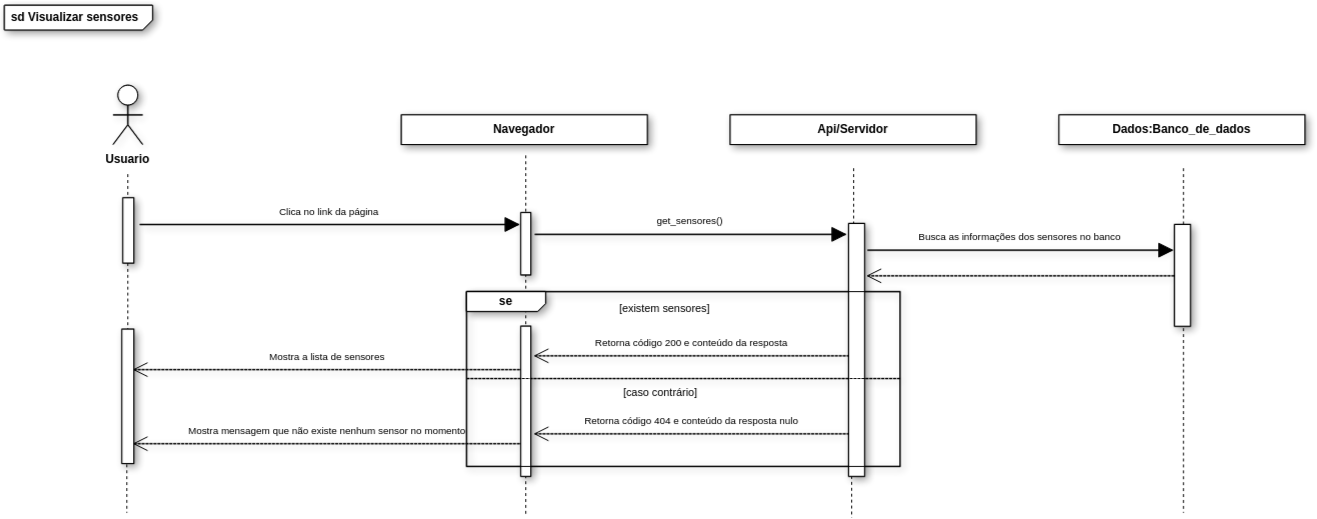
\includegraphics[scale=.3]{assets/sd_visualizarsensores.png}
  \caption{Diagrama de sequência para o caso de uso de visualizar sensores}
  \label{sdvisualizarsensores}
\end{figure}
\newpage

No caso do diagrama de sequência para visualizar os sensores que vemos na figura \ref{sdvisualizarsensores}, o usuário acessaria a página de sensores no navegador, em seguida, o navegador faria uma requisição utilizando o método GET para a API. A API, por sua vez, buscaria os dados dos sensores no banco de dados e, caso haja algum sensor cadastrado, retornaria o código de resposta HTTP 200 juntamente com a lista de sensores no corpo da resposta. Em seguida, os sensores seriam exibidos na tela para o usuário. Por outro lado, caso não haja nenhum sensor cadastrado no banco de dados, a API retornaria o código de resposta HTTP 404, com uma mensagem informando que não existem sensores no momento e o navegador mostraria essa mensagem para o usuário.

Com base nos diagramas de sequência apresentados nesta seção, é possível concluir que eles são importantes para compreender o comportamento do sistema e podem servir como base para o desenvolvimento eficiente e eficaz da plataforma. A correta implementação das funcionalidades e a satisfação dos usuários são garantidas por meio desses diagramas, que contribuem para uma compreensão clara do funcionamento do sistema.


\subsection{Diagrama Entidade Relacionamento}
\label{sec:entidaderelacionameto}
Conforme \citet{ELMASRI:2010} e  \citet{Silberschatz:2010}, um diagrama entidade relacionamento (DER) é uma ferramenta utilizada na modelagem de dados, que permite representar as entidades de um sistema e as relações entre elas. Isso ajuda a identificar possíveis problemas e inconsistências na estrutura do sistema, permitindo que sejam realizadas correções antes da implementação. Além disso, os diagramas de entidade-relacionamento também são utilizados para a documentação do sistema, facilitando o entendimento da plataforma.

Com base na notação descrita anteriormente, é possível visualizar o DER (Diagrama de Entidade e Relacionamento) da nossa plataforma na figura \ref{der}.

\begin{figure}[htbp]
  \centering 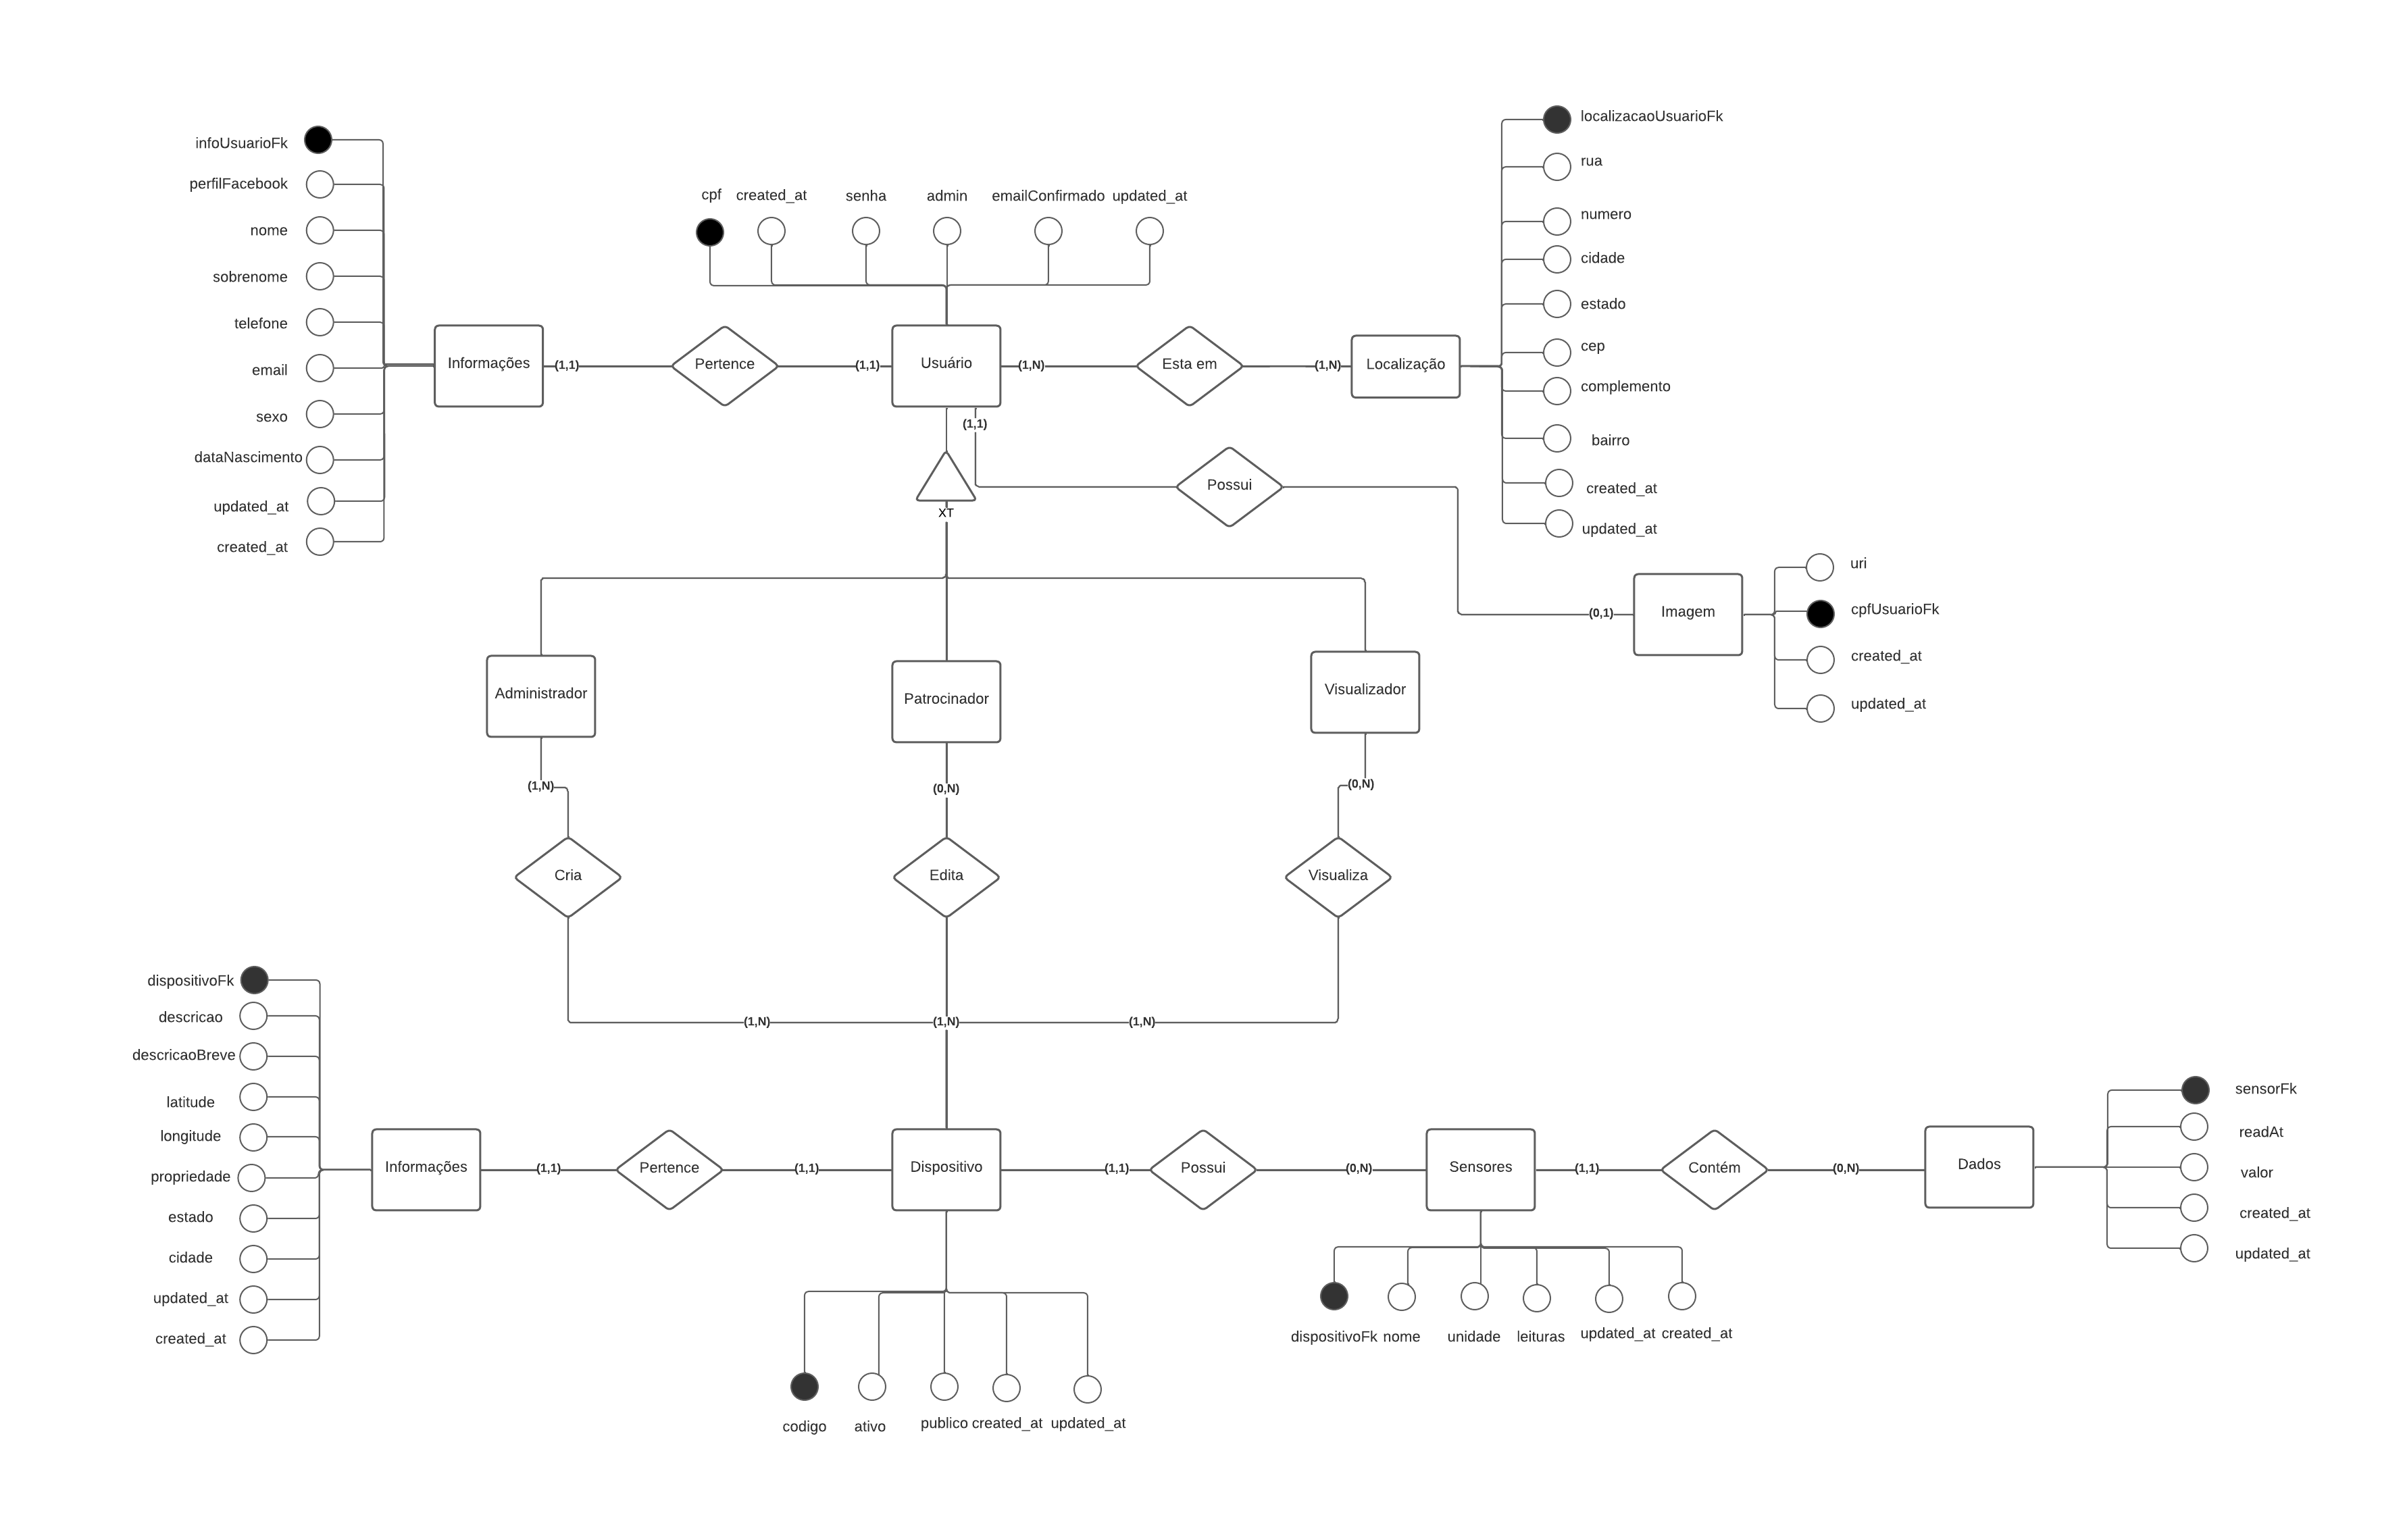
\includegraphics[scale=.275]{assets/DiagramaER.png}
  \caption{Diagrama Entidade Relacionamento}
  \label{der}
\end{figure}


No nosso diagrama, temos um total de 10 entidades distintas. Essas entidades são: Usuário, Administrador, Patrocinador, Visualizador, Informações, Localização, Imagem, Dispositivo, Sensores e Dados. Utilizamos a notação XT para representar uma relação de generalização/especialização total exclusiva entre as entidades Administrador, Patrocinador e Visualizador com a entidade genérica Usuário. Isso significa que todo usuário será classificado como Administrador, Patrocinador ou Visualizador. Vale ressaltar que algumas entidades são consideradas fracas, pois dependem de outras entidades para serem identificadas, como é o caso de Informações, Localização e Dados.

Dessa forma, a partir da modelagem dos dados, é possível definir os atributos e entidades específicas que serão armazenados em um banco de dados. Essa modelagem permite ter uma visão clara de como o banco de dados será estruturado na aplicação, possibilitando uma melhor compreensão do funcionamento do sistema.

\subsection{Modelo Lógico}
O modelo lógico de banco de dados é uma representação estruturada dos dados em uma aplicação, que define as entidades, atributos e relacionamentos entre elas. Segundo \citet{Silberschatz:2010}, o objetivo principal do modelo lógico é garantir a integridade e a consistência dos dados armazenados, além de permitir uma fácil manipulação dos mesmos.

Apesar de terem uma relação direta, o modelo lógico e o diagrama de entidade-relacionamento (DER) apresentado na seção \ref{sec:entidaderelacionameto} são conceitos distintos no campo da modelagem de dados. O modelo lógico é uma representação abstrata dos dados, independente de detalhes de implementação, como tipos de dados específicos ou sintaxe de consulta de um banco de dados em particular. Assim, o modelo lógico permite uma modelagem mais próxima do código em um banco de dados, possibilitando uma representação mais concreta e estruturada dos dados em questão.

Através da figura \ref{modelologico}, é possível visualizar a representação do banco de dados da plataforma na forma de um modelo lógico.
\begin{figure}[htbp]
  \centering 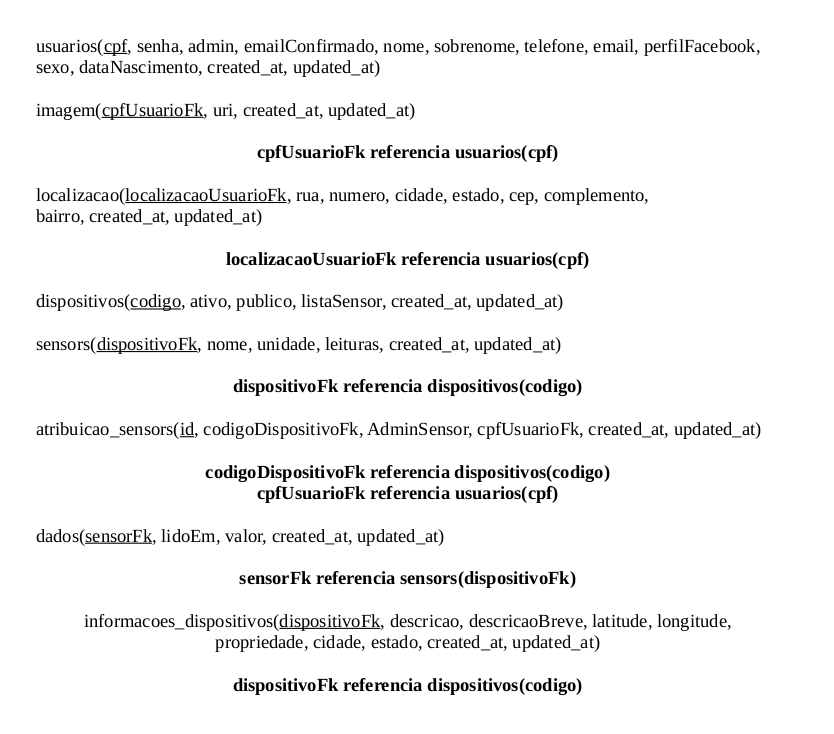
\includegraphics[scale=.4]{assets/modelo_logico.png}
  \caption{Modelo Lógico do Banco de Dados}
  \label{modelologico}
\end{figure}

Os atributos sublinhados representam as chaves primárias, sendo a tabela indicada à frente dos parênteses e seus atributos listados dentro dos mesmos. As chaves estrangeiras e suas relações são destacadas em negrito, na forma de "chave estrangeira referencia tabela(atributo)".

Em conclusão, o modelo lógico é uma ferramenta essencial para a implementação de um banco de dados eficiente e consistente em nossa aplicação. Ele nos permite visualizar a estrutura do banco de dados de forma abstrata, sem depender de uma linguagem específica de SQL, o que facilita a compreensão das relações entre as entidades e atributos. Com um modelo lógico bem definido, temos uma base sólida para a construção de um banco de dados que atenda às necessidades da aplicação, garantindo a integridade e qualidade dos dados armazenados.

\subsection{Diagrama de componentes}
Um diagrama de componentes tem como objetivo descrever a estrutura física do sistema, indicando quais são os componentes que o constituem, bem como as interfaces e dependências entre eles. De acordo com \citet{LARMAN:2011}, o diagrama de componentes é especialmente útil para a modelagem de sistemas distribuídos e de grande porte, onde a separação entre componentes é fundamental para garantir a escalabilidade e a manutenibilidade do sistema.

Os componentes no diagrama de componentes podem representar desde módulos de software até equipamentos de hardware, dependendo do nível de abstração que se deseja alcançar \cite{OMG:2017}. Segundo \citet{LARMAN:2011}, os componentes são elementos reutilizáveis e independentes, que podem ser substituídos ou atualizados sem afetar o resto do sistema. Por essa razão, o diagrama de componentes é frequentemente utilizado na arquitetura baseada em componentes, que visa a construção de sistemas a partir de componentes preexistentes e padronizados.

Na Figura \ref{diagramacomponentes}, é possível visualizar o diagrama de componentes da plataforma, onde utilizamos caixas para separar os componentes em front-end, back-end e banco de dados. No front-end, os componentes são representados como páginas web, descritos na linguagem escolhida para a implementação, enquanto no back-end, os componentes são descritos como classes na linguagem selecionada, além de um componente que representa o firmware responsável pelo sistema físico do sensor. No banco de dados, os componentes são representados como tabelas, e também é utilizado um componente descrito como um sistema gerenciador de banco de dados.
\begin{figure}[htbp]
  \centering 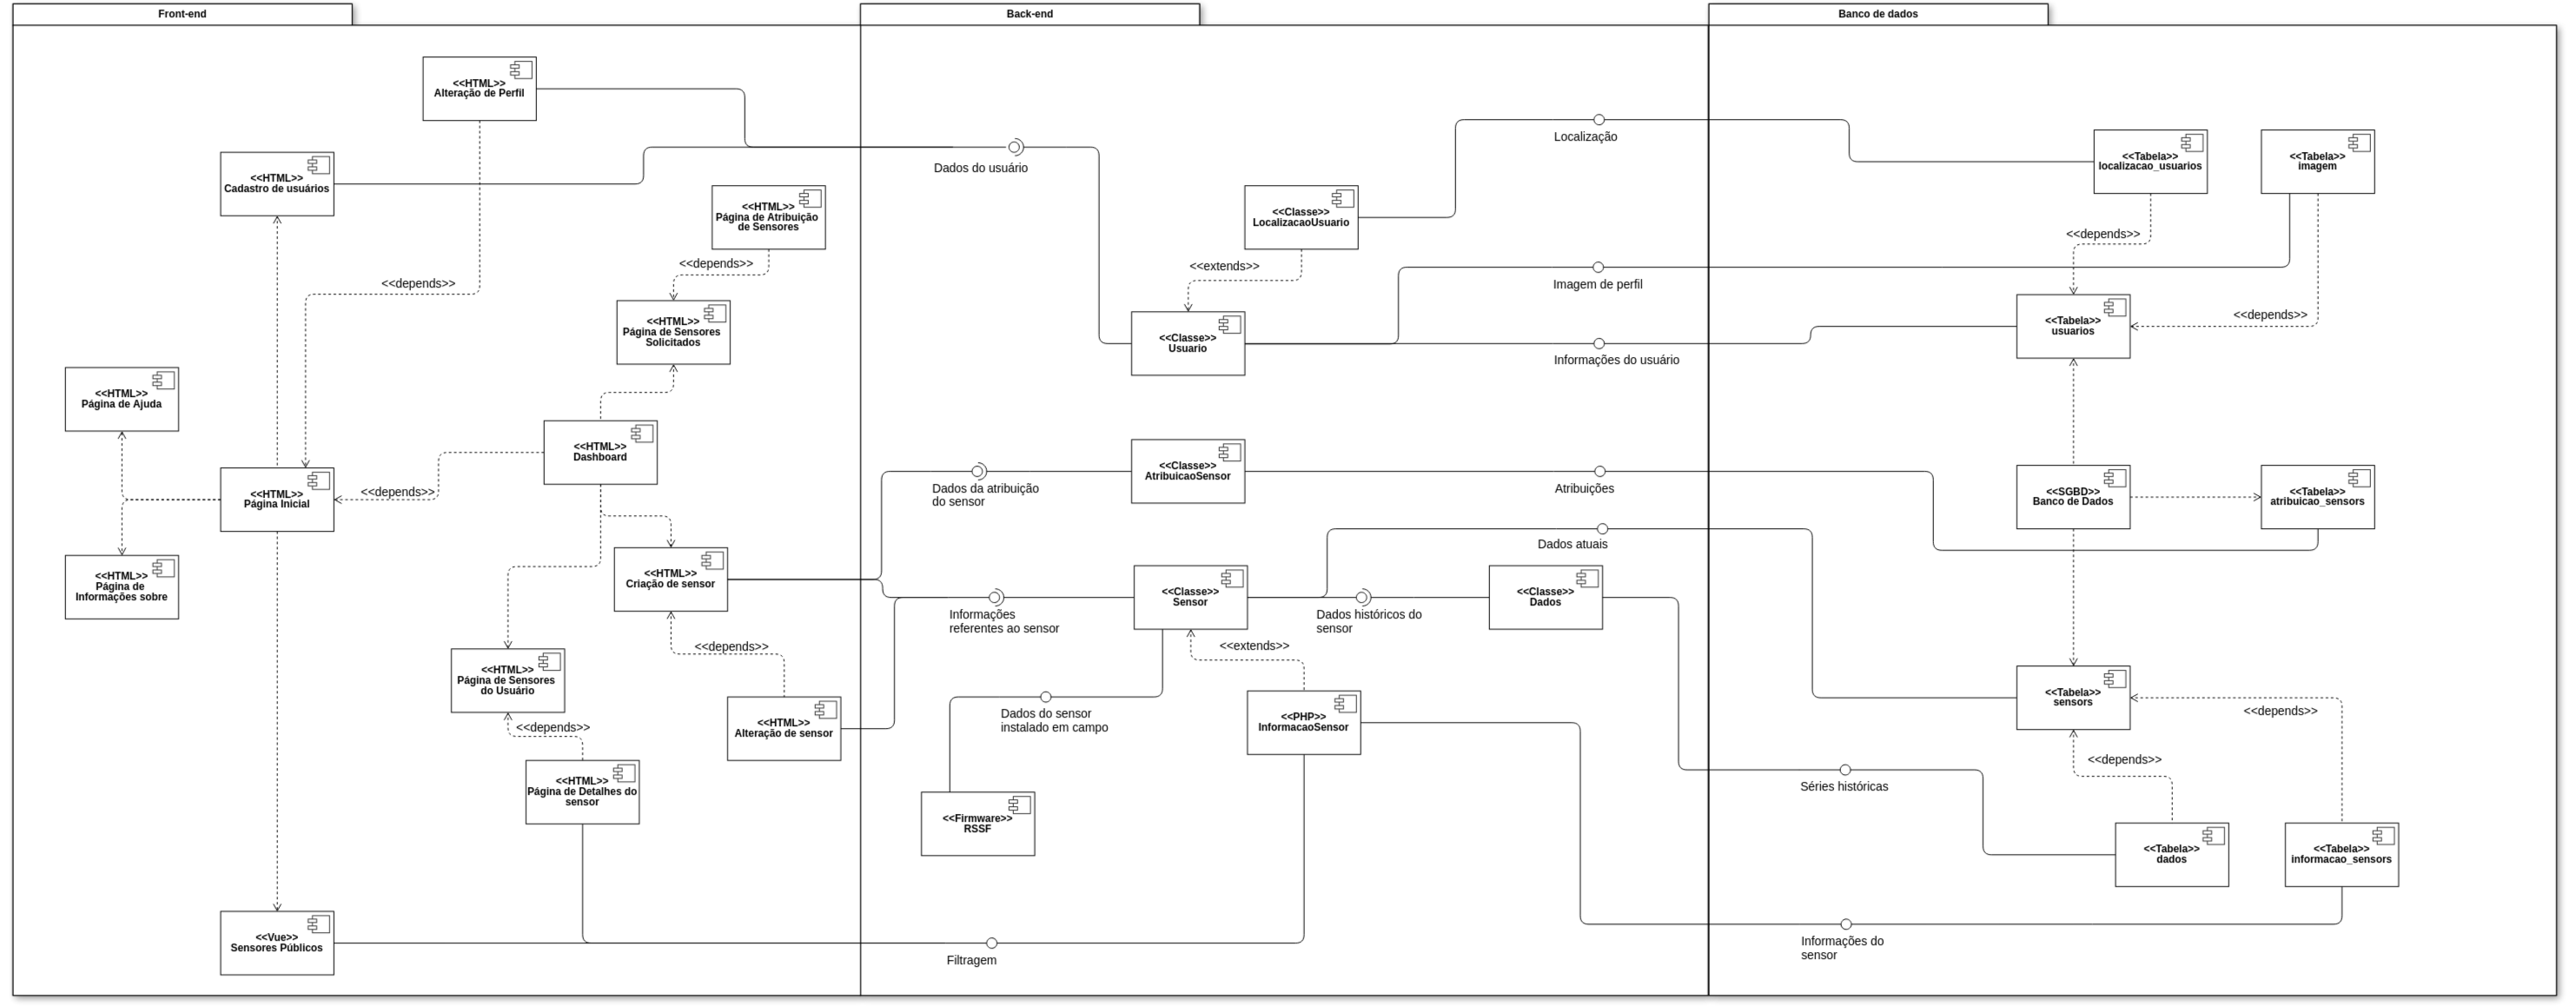
\includegraphics[scale=.165]{assets/componentes.png}
  \caption{Diagrama de Componentes}
  \label{diagramacomponentes}
\end{figure}
\newpage

No diagrama de componentes, é possível observar as interfaces requeridas e fornecidas pelos componentes, bem como as dependências entre eles. A notação <<extends>> é utilizada para representar que um componente herda de uma classe de outro componente, principalmente no back-end, onde os componentes são representados por classes. Na caixa do front-end, alguns componentes apresentam a notação <<depends>>, indicando que dependem de outros componentes. Por exemplo, as páginas de dashboard, alteração de perfil, criação de sensor, sensores do usuário, alteração de sensor e detalhes do sensor dependem da página de dashboard. Por sua vez, a página de dashboard depende da página de login, uma vez que esses componentes precisam ser acessados em sequência.

Dessa forma, ao utilizar o diagrama de componentes na modelagem da plataforma, foi possível obter uma representação visual clara e organizada das páginas a serem criadas e da estrutura física do sistema. Esse tipo abordagem permite identificar os diferentes componentes do sistema, suas interações e dependências, facilitando a compreensão holística do projeto. Além disso, o diagrama de componentes é uma ferramenta valiosa na identificação de problemas de design e possibilita ajustes e melhorias antes da implementação, oferecendo uma visão abrangente e detalhada da arquitetura do sistema. Essa perspectiva aprofundada pode contribuir significativamente para o desenvolvimento e manutenção da plataforma, tornando-a mais eficiente e confiável.

\subsection{Diagrama de implantação}
De acordo com \citet{LARMAN:2011}, o diagrama de implantação é importante para a compreensão da arquitetura física de um sistema, especialmente em sistemas distribuídos ou em nuvem. Ele permite identificar a localização dos componentes do sistema e como eles interagem entre si. Isso pode ajudar na tomada de decisões de arquitetura, como a escolha do hardware ou a otimização da rede.

O diagrama de implantação também pode ser útil na identificação de possíveis pontos de falha no sistema. Por exemplo, se um componente crítico estiver localizado em um único servidor, sem redundância ou backup, isso pode representar um ponto fraco no sistema. O diagrama de implantação pode ajudar a planejar a redundância, a escalabilidade e a tolerância a falhas em um sistema. \cite{OMG:2017}

Na figura \ref{diagramaimplantacao}, é possível visualizar uma representação simplificada do diagrama de implantação da plataforma, em que a área preenchida com a cor salmão representa o serviço de hospedagem em algum tipo de serviço na nuvem.

\begin{figure}[htbp]
  \centering 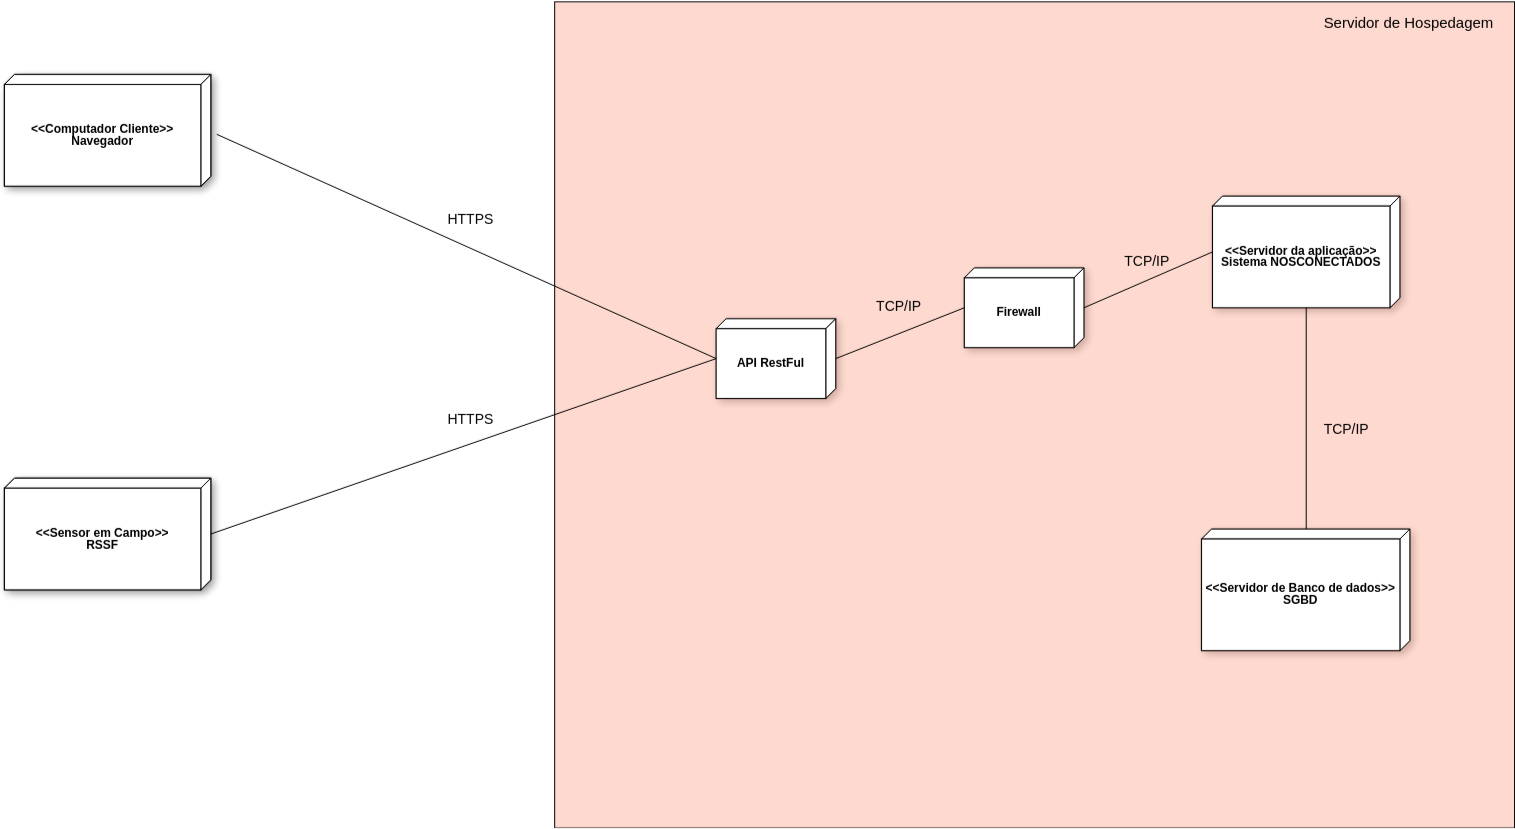
\includegraphics[scale=.3]{assets/diagramaimplantacao.png}
  \caption{Diagrama de Implantação}
  \label{diagramaimplantacao}
\end{figure}

O nó que representa o cliente se refere ao navegador, podendo ser qualquer dispositivo, seja ele móvel ou desktop. Esse nó se comunica com o nó da API RestFul através do protocolo HTTP, com a camada de segurança do socket HTTPS. O HTTPS é responsável por implementar a criptografia dos dados transmitidos entre o cliente e o servidor, garantindo que somente o cliente e o servidor possam ter acesso a esses dados. Além disso, o HTTPS ajuda a garantir a autenticidade do servidor, evitando possíveis ataques de phishing que possam enganar os usuários ao se passar por um site legítimo.

A API RestFul, por sua vez, se comunica com o Firewall do serviço de hospedagem através do protocolo TCP/IP, que se comunica com o servidor web da aplicação do NosConectados também pelo protocolo TCP/IP. Embora não tenha sido especificado, o servidor utilizado é do tipo Apache, escolhido pelo autor devido à sua familiaridade e experiência com esse tipo de servidor. O servidor web, então, se comunica com o sistema gerenciador de banco de dados através do protocolo TCP/IP.

O mesmo processo ocorre com os sensores, em que a rede de sensor se comunica com a API RestFul pelo protocolo HTTPS, que se comunica com o firewall pelo TCP/IP, que se comunica com o web server com o TCP/IP, que por sua vez, também se comunica com o SGBD através do protocolo TCP/IP.

Em resumo, o diagrama de implantação é uma ferramenta valiosa para a modelagem e a análise da arquitetura física de sistemas distribuídos ou em nuvem. Ele pode ajudar na tomada de decisões de arquitetura, na identificação de possíveis pontos de falha e na definição de requisitos de hardware e rede.

\section{Desenvolvimento}
\label{sec:desenvolvimento}
A fase de desenvolvimento da plataforma corresponde ao momento em que os requisitos previamente levantados são transformados em um produto de software funcional. Na visão de \citet{SOMMERVILLE:2011}, essa etapa envolve a codificação, a integração e os testes do software, e é uma das fases mais críticas do processo de desenvolvimento.

Durante esta etapa, o software é implementado por meio de uma linguagem de programação, seguindo as especificações detalhadas que foram definidas nas fases de análise de requisitos e modelagem, descritas nas seções \ref{sec:analiserequisitos} e \ref{sec:modelagem}, respectivamente. Segundo \citet{PRESSMAN:2016}, essa fase também pode incluir atividades como a documentação do código e a realização de testes, para garantir que o software esteja funcionando de acordo com as especificações.

A fase inicial do desenvolvimento da plataforma consiste em apresentar uma visão geral do projeto, incluindo as linguagens e ferramentas utilizadas em cada camada da implementação. São detalhadas as ferramentas, frameworks, bibliotecas e linguagens de programação que foram empregadas para alcançar as funcionalidades finais do sistema, bem como as definições das camadas do sistema, front-end e back-end. Essa seção fornece uma visão panorâmica do cenário tecnológico e arquitetural do projeto, destacando as escolhas feitas para a sua implementação.

Em seguida, é apresentado o desenvolvimento do banco de dados, baseado na modelagem previamente descrita. Nessa seção, são apresentados detalhes sobre a estrutura das tabelas do banco de dados, ressaltando as relações entre elas, a escolha do sistema gerenciador do banco, as chaves primárias e estrangeiras, entre outros elementos. É explicado como a modelagem de dados foi implementada no banco de dados real do sistema, garantindo a consistência e a integridade dos dados armazenados.

Uma seção específica é dedicada à API, que é um componente fundamental da plataforma. Nessa seção, é explicado o conceito de API e como ela foi implementada para possibilitar a integração de diferentes sistemas e serviços. São detalhadas as funcionalidades oferecidas pela API, incluindo as operações disponíveis, os formatos de dados utilizados nas requisições e respostas, e as medidas de autenticação e autorização implementadas para garantir a segurança e a privacidade dos dados transmitidos.

Adicionalmente são mencionadas as APIs públicas que são consumidas pela plataforma, evidenciando como foi realizada a integração e quais serviços são acessados por meio dessas APIs. Os pontos de acesso disponibilizados pela API, conhecidos como endpoints, são detalhados na mesma seção onde a API é apresentada, demonstrando os resultados do desenvolvimento e como esses endpoints foram implementados com base nessa etapa do projeto.

Essa seção é essencial para compreender a importância da API na arquitetura da plataforma e como ela possibilita a interconexão de diferentes sistemas, serviços e funcionalidades. A explicação detalhada das funcionalidades oferecidas pela API, bem como as medidas de segurança implementadas, ressalta o cuidado em garantir a confiabilidade e a proteção dos dados transmitidos pela plataforma. Além disso, a menção das APIs públicas consumidas pela plataforma destaca a capacidade de integração da plataforma com outros serviços e sistemas externos, o que amplia suas possibilidades e recursos disponíveis. 

Outro aspecto abordado é a autenticação de usuários e sensores, com uma subseção específica para tratar desse tema. São detalhados os mecanismos de autenticação implementados, tais como login e senha, tokens de acesso, entre outros. É explicado como esses mecanismos foram desenvolvidos e integrados ao sistema, garantindo a segurança e a proteção das informações dos usuários e dos sensores conectados à plataforma.

Além disso, é apresentado como foram desenvolvidos os gráficos que exibem as séries históricas da plataforma. São detalhadas as bibliotecas e ferramentas utilizadas para criar os gráficos, os tipos de gráficos disponíveis na plataforma, as opções de personalização oferecidas aos usuários, e como os dados são processados e apresentados de forma visualmente atrativa e compreensível aos usuários.

Outra seção de destaque é o controle de administração para os diferentes tipos de usuários da plataforma, como administradores, moderadores e usuários comuns. É detalhado como foram implementadas as restrições de acesso e os privilégios de cada tipo de usuário, garantindo a segurança e a integridade do sistema. Também são destacadas as funcionalidades oferecidas aos usuários administradores, tais como gerenciamento de usuários, configurações avançadas, entre outras.

As camadas de segurança também são abordadas, destacando como foram implementadas as medidas de proteção dos dados sensíveis.
\subsection{Front-end}
No desenvolvimento do front-end, onde é criada a interface com a qual o usuário interage diretamente, é essencial considerar os conceitos de UI/UX (User Interface/User Experience) para proporcionar uma experiência agradável e intuitiva. Para isso, utilizamos ferramentas e linguagens de programação que implementam as funcionalidades do sistema para o usuário. Utilizamos o Vue.js \cite{vue:2014}, juntamente com o Buefy \cite{buefy:2022} e o Bulma \cite{bulma:2022}, que nos ofereceram uma interface limpa, de boa aparência e segura em termos de usabilidade.

Além disso, utilizamos o Leaflet.js \cite{leaflet:2023}, uma biblioteca JavaScript de código aberto, para a criação de mapas interativos, e o Apexcharts.js \cite{ApexCharts:2022} para os dashboards, exibindo os dados históricos dos sensores em gráficos. Essa integração permitiu apresentar os dados de forma visual e intuitiva para os usuários, facilitando a compreensão das informações coletadas pelos sensores.

O Bootstrap \cite{bootstrap:2023}, um framework front-end de código aberto, também foi utilizado para auxiliar na responsividade da aplicação, garantindo que ela seja exibida corretamente em diferentes dispositivos e tamanhos de tela. Em conjunto com o Bulma e o Buefy, o Bootstrap complementou as ferramentas utilizadas para o desenvolvimento de uma interface de usuário moderna e responsiva.
\begin{itemize}
    \item Vue.js: Framework JavaScript open source para a criação de plataformas web, que nos permite criar aplicações de forma reativa com foco na interação e experiência do usuário. Conta com uma arquitetura bem estruturada por meio da criação de componentes reusáveis. Muito utilizado para criar aplicações SPA, e atualmente um dos frameworks Javascript para criação de interfaces mais populares do mundo, de acordo com a pesquisa do Stack Overflow 2021 Developer \cite{stackoverflow:2022}.
    \item Bootstrap: Framework front-end de código aberto amplamente utilizado para o desenvolvimento de interfaces web responsivas e modernas. Oferece um conjunto completo de estilos e componentes pré-definidos, facilitando a criação de layouts e a implementação de recursos interativos em aplicações web.
    \item Bulma: Framework CSS inspirado no Bootstrap e baseado em Flexbox, totalmente responsivo e open source.
    \item Buefy: Biblioteca de componentes UI responsivos baseados no Bulma com um conjunto completo de componentes com aplicação focada em dashboards, com recursos de customização e tratativas de eventos.
    \item Leaflet.js: Biblioteca JavaScript de código aberto para criação de mapas interativos em aplicações web.
    \item Apexcharts.js: Biblioteca JavaScript de código aberto para criação de gráficos interativos para plotagem de dashboards.
\end{itemize}
\subsection{Back-end}
O back-end é responsável por tudo o que está por trás da plataforma, sendo a parte do desenvolvimento que não é diretamente acessível ou interativa para o usuário. Para a criação do banco de dados e a programação do servidor, utilizamos o MySQL \cite{mysql:2022} como sistema gerenciador de banco de dados relacional, em conjunto com o PHP \cite{PHP:2022} como linguagem de programação voltada para o desenvolvimento de aplicações web no lado do servidor. Para realizar a conexão com o banco de dados, utilizamos o PDO \cite{PDO:2022}, uma interface de conexão a banco de dados em PHP. Além disso, utilizamos o Slim Framework \cite{slim:2023}, um framework PHP de código aberto, para a criação das rotas da API, permitindo um desenvolvimento eficiente e organizado das funcionalidades do back-end.
\begin{itemize}
    \item MySQL: Sistema gerenciador de banco de dados relacional de código aberto usado na maioria das aplicações gratuitas para gerir suas bases de dados. O serviço utiliza a linguagem SQL, que é a linguagem mais popular para inserir, acessar e gerenciar o conteúdo armazenado num banco de dados de acordo com a pesquisa do Stack Overflow 2021 Developer \cite{stackoverflow:2022}. 
    \item PHP: Linguagem de script open source de uso geral, muito utilizada no back-end, e especialmente adequada para o desenvolvimento web. 
    \item PDO: Extensão da linguagem PHP para acesso a banco de dados. Totalmente orientado a objetos, seguindo o paradigma de POO, permitindo a definição uma interface de conexão a um banco de dados.
    \item Slim Framework: Framework PHP minimalista e de código aberto para desenvolvimento de APIs e aplicações web eficientes e rápidas, com recursos como rotas, gerenciamento de requisições e respostas, validação de dados e autenticação.
\end{itemize}
\subsection{API}
Para conectar as informações dos sensores localizados em campo com nossa base de dados e garantir a segurança na conexão entre o front-end e o back-end, implementamos uma API que recebe as informações em formato JSON e as envia para nossa base de dados. Além disso, utilizamos o conceito de CRUD (Create, Read, Update, Delete) para permitir que o usuário insira, delete ou atualize informações por meio da plataforma, enviando as informações por meio das rotas da API para a base de dados usando os métodos POST, PUT e DELETE.

No front-end, a obtenção de dados também é realizada por meio de rotas da API, porém utilizando o método GET, estabelecendo assim a conexão segura entre o back-end e o front-end através do protocolo HTTP. Essa estratégia foi adotada para garantir uma experiência fluida e segura para o usuário. Nossa plataforma também consome APIs públicas, como a API do IBGE \cite{IBGE:2022}, que contém informações sobre localidades de cidades e estados do Brasil. Dessa forma, garantimos uma escolha precisa e evitamos possíveis erros de localização no registro.

A Figura \ref{apinos} apresenta um fluxograma que ilustra a conexão das RSSFs com a base de dados, back-end e front-end, demonstrando a importância do uso de APIs para conectar os diferentes componentes do sistema de forma eficiente e segura.

\begin{figure}[htbp]
\centering 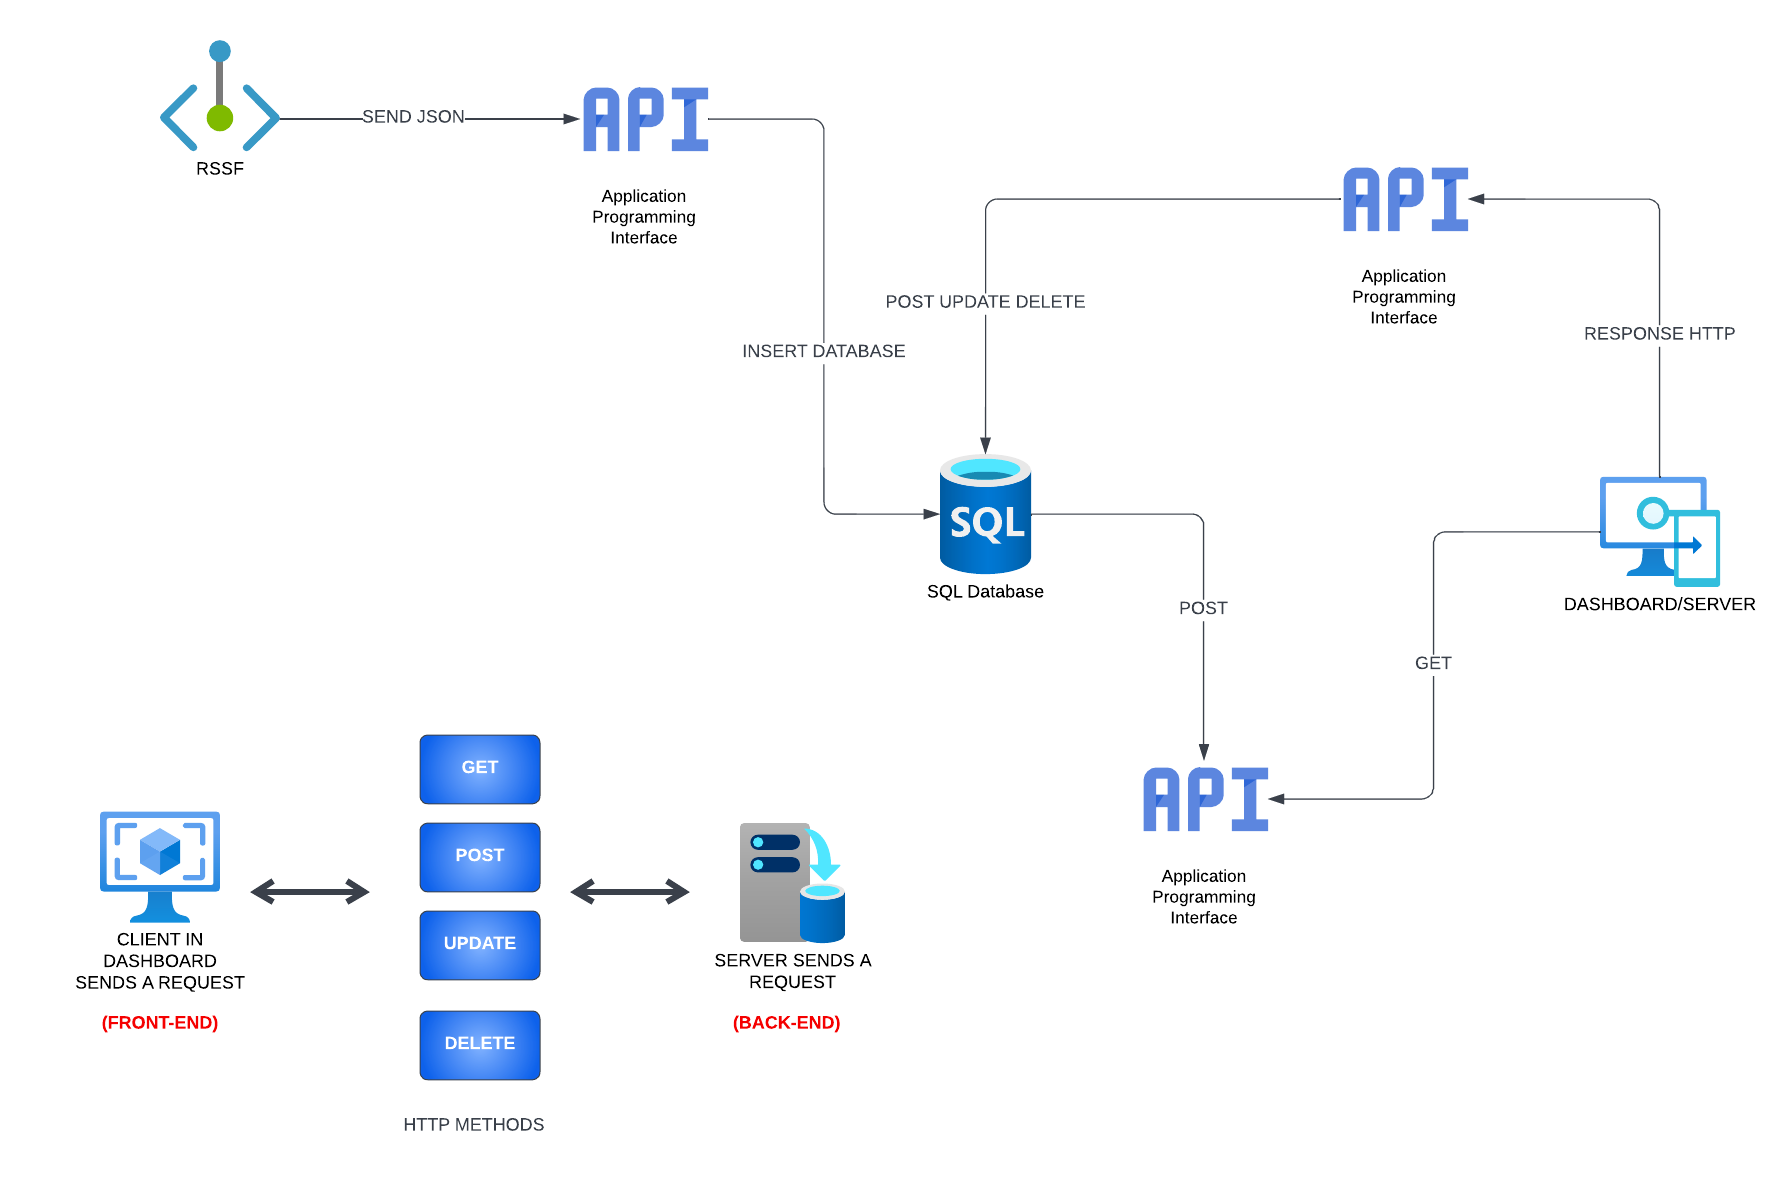
\includegraphics[scale=.4]{assets/apinos.png}
\caption{Representação da API da plataforma}
\label{apinos}
\end{figure}

Durante o processo de desenvolvimento da API, o Postman \cite{Postman:2023} tornou-se uma ferramenta indispensável para a realização de testes de requisições. Com sua ampla gama de recursos, foi possível executar uma série de testes simulando cenários diversos que poderiam ocorrer em um ambiente de produção, verificando a validade das respostas e detectando e solucionando possíveis problemas. Ademais, o Postman também exerceu um papel fundamental na documentação da API, permitindo a geração automática de documentação a partir das requisições realizadas. Assim, foi possível fornecer aos usuários uma documentação completa e atualizada da API, simplificando a compreensão e utilização da mesma. Na figura \ref{postman}, é possível visualizar uma captura de tela do Postman em uma das rotas disponíveis na API da plataforma.
\begin{figure}[htbp]
\centering 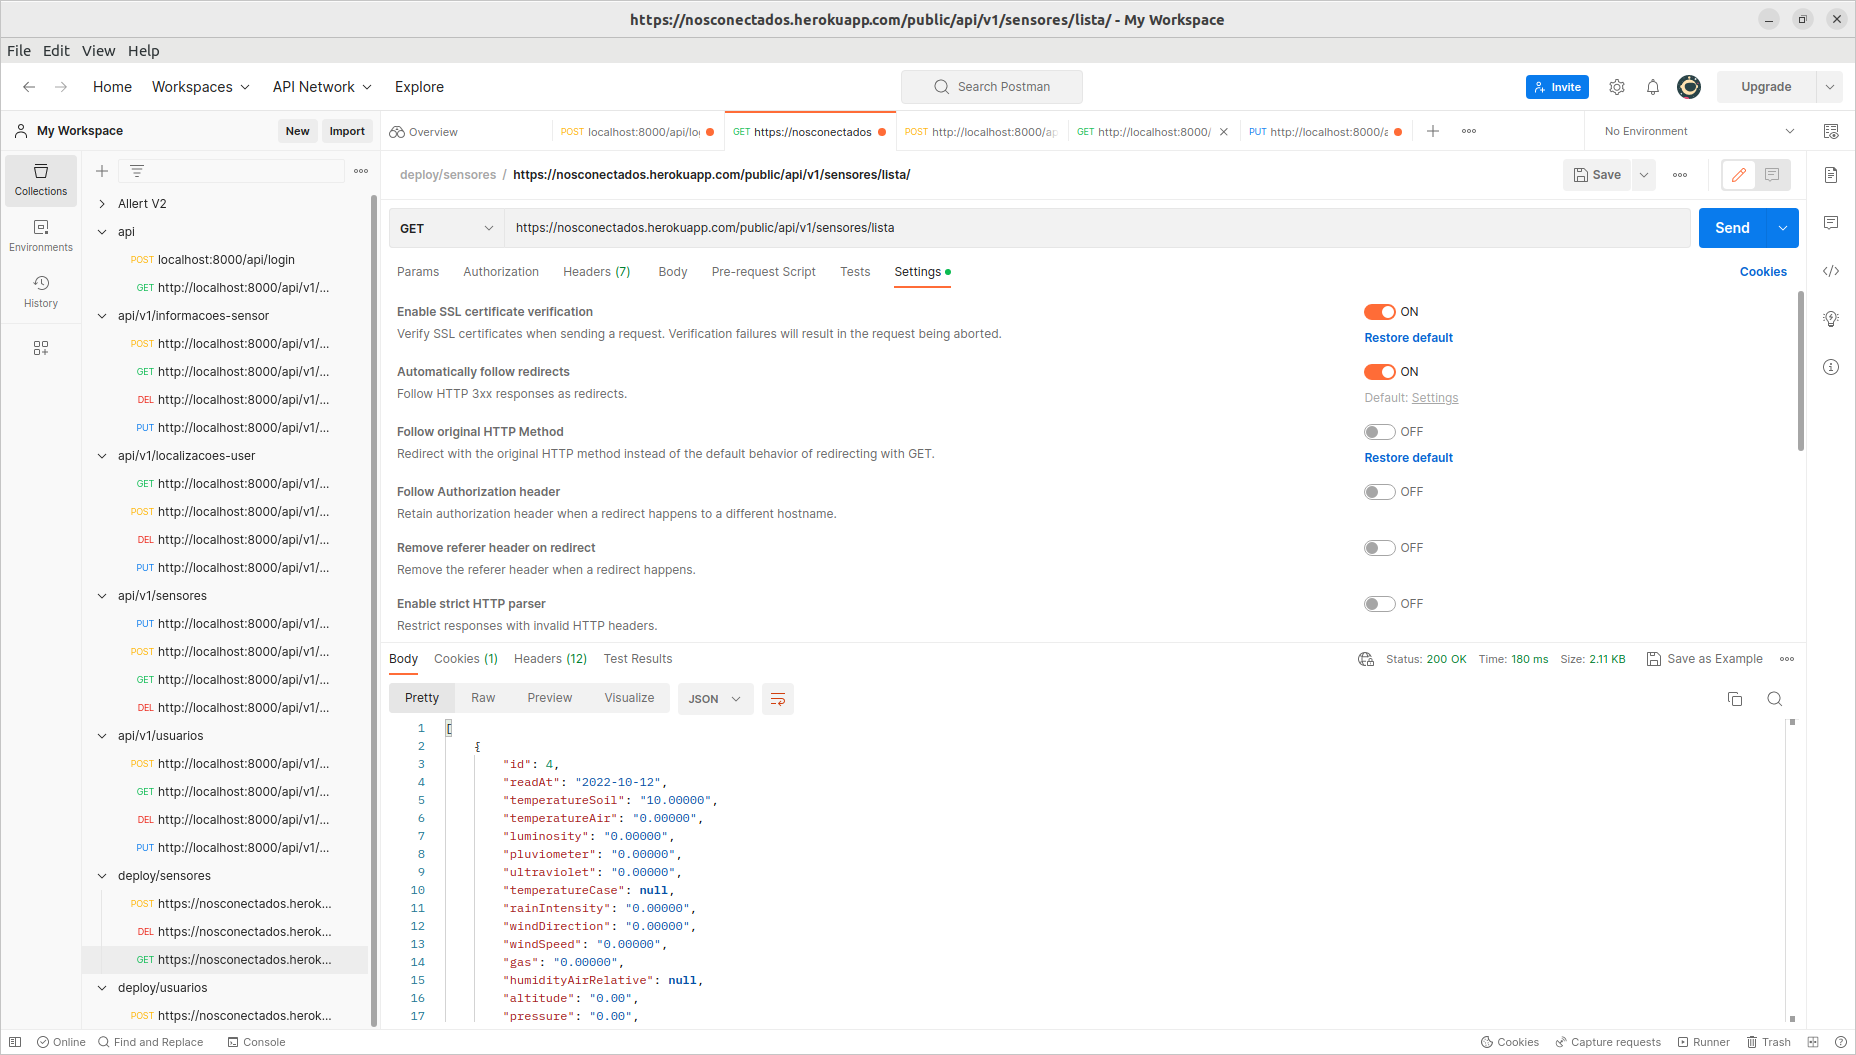
\includegraphics[scale=.25]{assets/postman.png}
\caption{Visão das rotas da API pelo Postman}
\label{postman}
\end{figure}
\newpage

Em virtude disso, a API desenvolvida é construída seguindo a arquitetura Restful (Representational State Transfer). Essa arquitetura é baseada em princípios simples, como a utilização de URIs para identificar recursos e a utilização de verbos HTTP para definir as ações a serem realizadas nesses recursos. Além disso, o Restful permite que as requisições sejam realizadas de forma independente do estado do servidor, tornando a comunicação mais eficiente.

A estrutura da API é composta por recursos que representam as entidades do sistema, como usuários, sensores, localizações, informações, atribuições e dados históricos. Cada recurso possui um conjunto de endpoints, que definem as operações que podem ser realizadas com aquele recurso, através de métodos do protocolo HTTP como GET, POST, PUT e DELETE.

Outro aspecto importante é a utilização de autenticação e autorização. Para garantir a segurança das informações, a API requer a autenticação do usuário através do envio de credenciais, por meio de um token. Além disso, é possível definir diferentes níveis de acesso para cada recurso, garantindo que apenas usuários autorizados possam acessar informações sensíveis.

Um dos principais benefícios da utilização de uma arquitetura Restful é a sua facilidade de integração com outras aplicações. A API do NosConectados, por exemplo, pode ser facilmente consumida por outras aplicações que utilizam a mesma arquitetura, sem a necessidade de conhecimento prévio sobre a implementação interna da aplicação. Além disso, a API também oferece suporte a formatos de dados do tipo JSON, o que torna a integração com outras plataformas e serviços ainda mais fácil e flexível.

A tabela \ref{tab:rotas-api} apresenta de forma clara e organizada as rotas disponíveis na API, juntamente com os verbos HTTP correspondentes, arquivos associados, parâmetros requeridos e uma breve descrição para cada uma dessas rotas.

\begin{table}[h]
\centering
\resizebox{\textwidth}{!}{\begin{tabular}{|c|l|l|l|p{7cm}|}
\hline
HTTP Verb & Rota & Parametros & Arquivo & Descrição \\
\hline
GET & / & & autenticacao.php & Mensagem de bem vindo a API \\
\hline
GET & /api/user\textbf{*} & & autenticacao.php & Obter os dados do usuário após login \\
\hline
GET & /api/sensor\textbf{*} & & autenticacao.php & Obter os sensores do usuário após login \\
\hline
GET & /api/token\textbf{** }& & autenticacao.php & Obter o token do usuário \\
\hline
POST & /api/login & email e senha & autenticacao.php & Gera um token caso o usuário esteja no banco de dados \\
\hline
GET & /api/v1/atribuicao/lista\textbf{**} & & atribuicao.php & Lista todas as atribuições \\
\hline
POST & /api/v1/atribuicao/adiciona\textbf{*} & cpf do usuário, codigo do dispositivo e tipo & atribuicao.php & Adiciona uma atribuição \\
\hline
GET & /api/v1/atribuicao/lista/\{id\}\textbf{*} & id da atribuição & atribuicao.php & Lista uma atribuição com determinado id \\
\hline
PUT & /api/v1/atribuicao/lista/\{id\}\textbf{*}  & id da atribuição & atribuicao.php & Atualiza uma atribuição com determinado id \\
\hline
DELETE & /api/v1/atribuicao/remove/\{id\}\textbf{*}  & id da atribuição & atribuicao.php & Remove uma atribuição com determinado id \\
\hline
GET & /api/v1/localizacoes-users/lista\textbf{**} & & localizacoes\_usuarios.php & Lista todas as localizações de todos os usuários \\
\hline
POST & /api/v1/localizacoes-users/adiciona\textbf{*} & todas as informações de localização e o cpf do usuário & localizacoes\_usuarios & Adiciona localização ao usuário \\
\hline
GET & /api/v1/localizacoes-users/lista/\{cpf\}\textbf{*} & cpf do usuário  & localizacoes\_usuarios.php & Lista uma localização com determinado id \\
\hline
\hline
PUT & /api/v1/localizacoes-users/atualiza/\{cpf\}\textbf{*} & cpf do usuário  & localizacoes\_usuarios & Atuaiza uma localização com determinado id \\
\hline
DELETE & /api/v1/localizacoes-users/remove/\{cpf\}\textbf{*} & cpf do usuário & localizacoes\_usuarios & Remove uma localização com determinado id \\
\hline
GET & /api/v1/sensores/lista/\textbf{**} & & sensores.php & Lista todos os dados de todos os sensores\\
\hline
GET & /api/v1/dispositivos/lista/publicos & & dispositivos.php & Lista todos os dados de todos os sensores públicos\\
\hline
POST & /api/v1/dispositivos/adiciona\textbf{*} & todos os dados do dispositivos & dispositivos.php & Adiciona um novo dispositivo\\
\hline
PUT & /api/v1/dispositivos/atualiza/\{codigo\}\textbf{*} & codigo do dispositivo & dispositivos.php & Atualiza os dados do dispositivo com determinado código\\
\hline
DELETE & /api/v1/dispositivos/remove/\{codigo\}\textbf{*} & codigo do dispositivo & dispositivos.php & Remove os dados do dispositivo com determinado código\\
\hline
GET & /api/v1/dispositivos/lista/\{codigo\}\textbf{*} & codigo do dispositivo & dispositivos.php & Lista os dados do dispositivo com determinado código\\
\hline
POST & /api/v1/sensores/adiciona\textbf{*} & todos os dados do sensor & sensores.php & Adiciona um novo sensor\\
\hline
PUT & /api/v1/sensores/atualiza/\{nome\}\textbf{*} & nome do sensor & sensores.php & Atualiza os dados do sensor com determinado nome\\
\hline
DELETE & /api/v1/sensores/remove/\{nome\}\textbf{*} & nome do sensor & sensores.php & Remove os dados do sensor com determinado nome\\
\hline
GET & /api/v1/sensores/lista/\{nome\}\textbf{*} & nome do sensor & sensores.php & Lista os dados de um sensor com determinado nome\\
\hline
GET & /api/v1/dispositivos/solicitados/\{cpf\}\textbf{*} & cpf do usuário do usuário & sensores.php & Lista os dispositivos solicitados para o cpf do usuário logado\\
\hline
GET & /api/v1/usuarios/lista\textbf{**} &  & usuarios.php & Lista todos os usuários\\
\hline
POST & /api/v1/usuarios/cadastro & todas as informações do usuário & usuarios.php & Adiciona um usuário (cadastro)\\
\hline
GET & /api/v1/usuarios/lista/\{cpf\}\textbf{*} & cpf do usuário & usuarios.php & Lista um usuário com determinado cpf\\
\hline
DELETE & /api/v1/usuarios/remove/\{cpf\}\textbf{*} & cpf do usuário & usuarios.php & Remove um usuário com determinado cpf\\
\hline
PUT & /api/v1/usuarios/atualiza/\{cpf\}\textbf{*} & cpf do usuário & usuarios.php & Atualiza um usuário com determinado cpf\\
\hline
GET & /api/v1/dados/lista/\{nome\}\textbf{*} & nome do sensor & dados.php & Lista a série histórica para sensor com determinado nome\\
\hline
GET & /api/v1/dados/lista/\textbf{**} & & dados.php & Lista todas as séries históricas de todos os sensores\\
\hline
DELETE & /api/v1/dados/remove/\{nome\}\textbf{**} & nome do sensor & dados.php & Remove a série histórica para sensor com determinado nome\\
\hline
\end{tabular}}
\caption{Tabela de rotas da API}
\label{tab:rotas-api}
\end{table}
\newpage
Rotas com \textbf{*} requerem autenticação, ou seja, o usuário deve estar logado no sistema e fornecer um token válido no cabeçalho da requisição. Algumas rotas, por sua vez, além de requererem autenticação só podem ser acessadas por usuários com privilégios de administrador, essas foram definidas com \textbf{**} na tabela.

Vale destacar que a tabela não possui uma rota para atualização de dados históricos do sensor. Isso ocorre para que mesmo um usuário administrador não possa alterar dados históricos. Também não há uma rota para criar um novo elemento na tabela de dados históricos, pois ao adicionar um novo sensor através da rota \verb|/api/v1/dispositivos/adicionar| ou atualizar um dispositivo através da rota \verb|/api/v1/dispositivos/atualizar/{codigo}|, uma cópia é adicionada automaticamente à tabela de dados históricos no banco de dados. 

Em conclusão, a API é um componente essencial na arquitetura da nossa plataforma, permitindo a integração e comunicação eficiente entre os diferentes sistemas de software. Utilizamos o protocolo HTTP padrão da web, para garantir uma interface padronizada e estruturada. Os formatos de dados utilizados nas requisições e respostas são em JSON, permitindo uma fácil manipulação e interoperabilidade entre os sistemas. Além disso, implementamos medidas de autenticação e autorização para garantir a segurança e privacidade dos dados transmitidos. Através de HTTPS e token-based authentication como é descrito na seção \ref{sec:autenticacao}, garantimos a proteção dos dados em trânsito, evitando acesso não autorizado. A utilização de APIs públicas confiáveis, como a API do IBGE, também contribui para a precisão e qualidade dos dados registrados na nossa plataforma. Essas medidas de segurança e a escolha cuidadosa dos formatos de dados e APIs utilizadas são fundamentais para garantir uma experiência fluida, segura e confiável para os usuários da plataforma.
\subsection{Banco de dados}
No âmbito deste trabalho, optou-se por utilizar o sistema de gerenciamento de banco de dados MySQL \cite{mysql:2022}, que é um sistema relacional de código aberto amplamente utilizado. Há vários estudos comparativos entre diferentes SGBDs, como o realizado por \citet{Delfino:2012}, que avaliou o desempenho de imagens médicas em três sistemas diferentes, concluindo que o MySQL apresentou resultados satisfatórios em termos de desempenho neste cenário. No entanto, embora existam vários cenários e cada um possa apresentar resultados diferentes, a escolha do MySQL para este trabalho deve-se principalmente à experiência prévia do autor com o sistema e à sua comprovada eficiência.

Ao utilizar esse sistema, é importante entender a sua arquitetura e as suas funcionalidades. De acordo com o seu manual, ele é composto por um servidor que executa em segundo plano e um cliente que se comunica com o servidor para executar as operações de banco de dados. Além disso, o sistema oferece uma variedade de recursos, como suporte a transações ACID, índices, chaves estrangeiras, armazenamento de blobs e muito mais \cite{mysql:2022}. 

Além de suas funcionalidades e eficiência, outra vantagem do sistema de gerenciamento de banco de dados MySQL \cite{mysql:2022} é sua compatibilidade com diversas linguagens de programação, incluindo a linguagem escolhida para o back-end da plataforma em questão: o PHP \cite{PHP:2022}. Essa compatibilidade facilita a integração do banco de dados com o restante do sistema, permitindo o acesso e manipulação dos dados armazenados através de consultas SQL. Além disso, o PHP possui uma ferramenta chamada PHPMyAdmin, que permite visualizar e gerenciar o banco de dados MySQL de maneira prática e intuitiva, sem a necessidade de escrever comandos SQL manualmente. Com o PHPMyAdmin, é possível criar, editar e excluir tabelas, inserir e alterar registros, além de executar consultas complexas e otimizar a estrutura do banco de dados. Isso torna o processo de gerenciamento do banco de dados mais simples e eficiente, contribuindo para a agilidade e qualidade do desenvolvimento da plataforma.


A Figura \ref{bancodedados} apresenta uma representação gráfica do banco de dados da plataforma, gerada pelo PHPMyAdmin. O retângulo verde nas caixas indica a chave primária e as setas indicam a ligação entre a chave estrangeira. Essa ferramenta é um software livre e de código aberto que permite a administração de bancos de dados MySQL \cite{mysql:2022}, tornando-se uma opção popular para gerenciamento de bancos de dados deste tipo. 

\begin{figure}[htbp]
  \centering 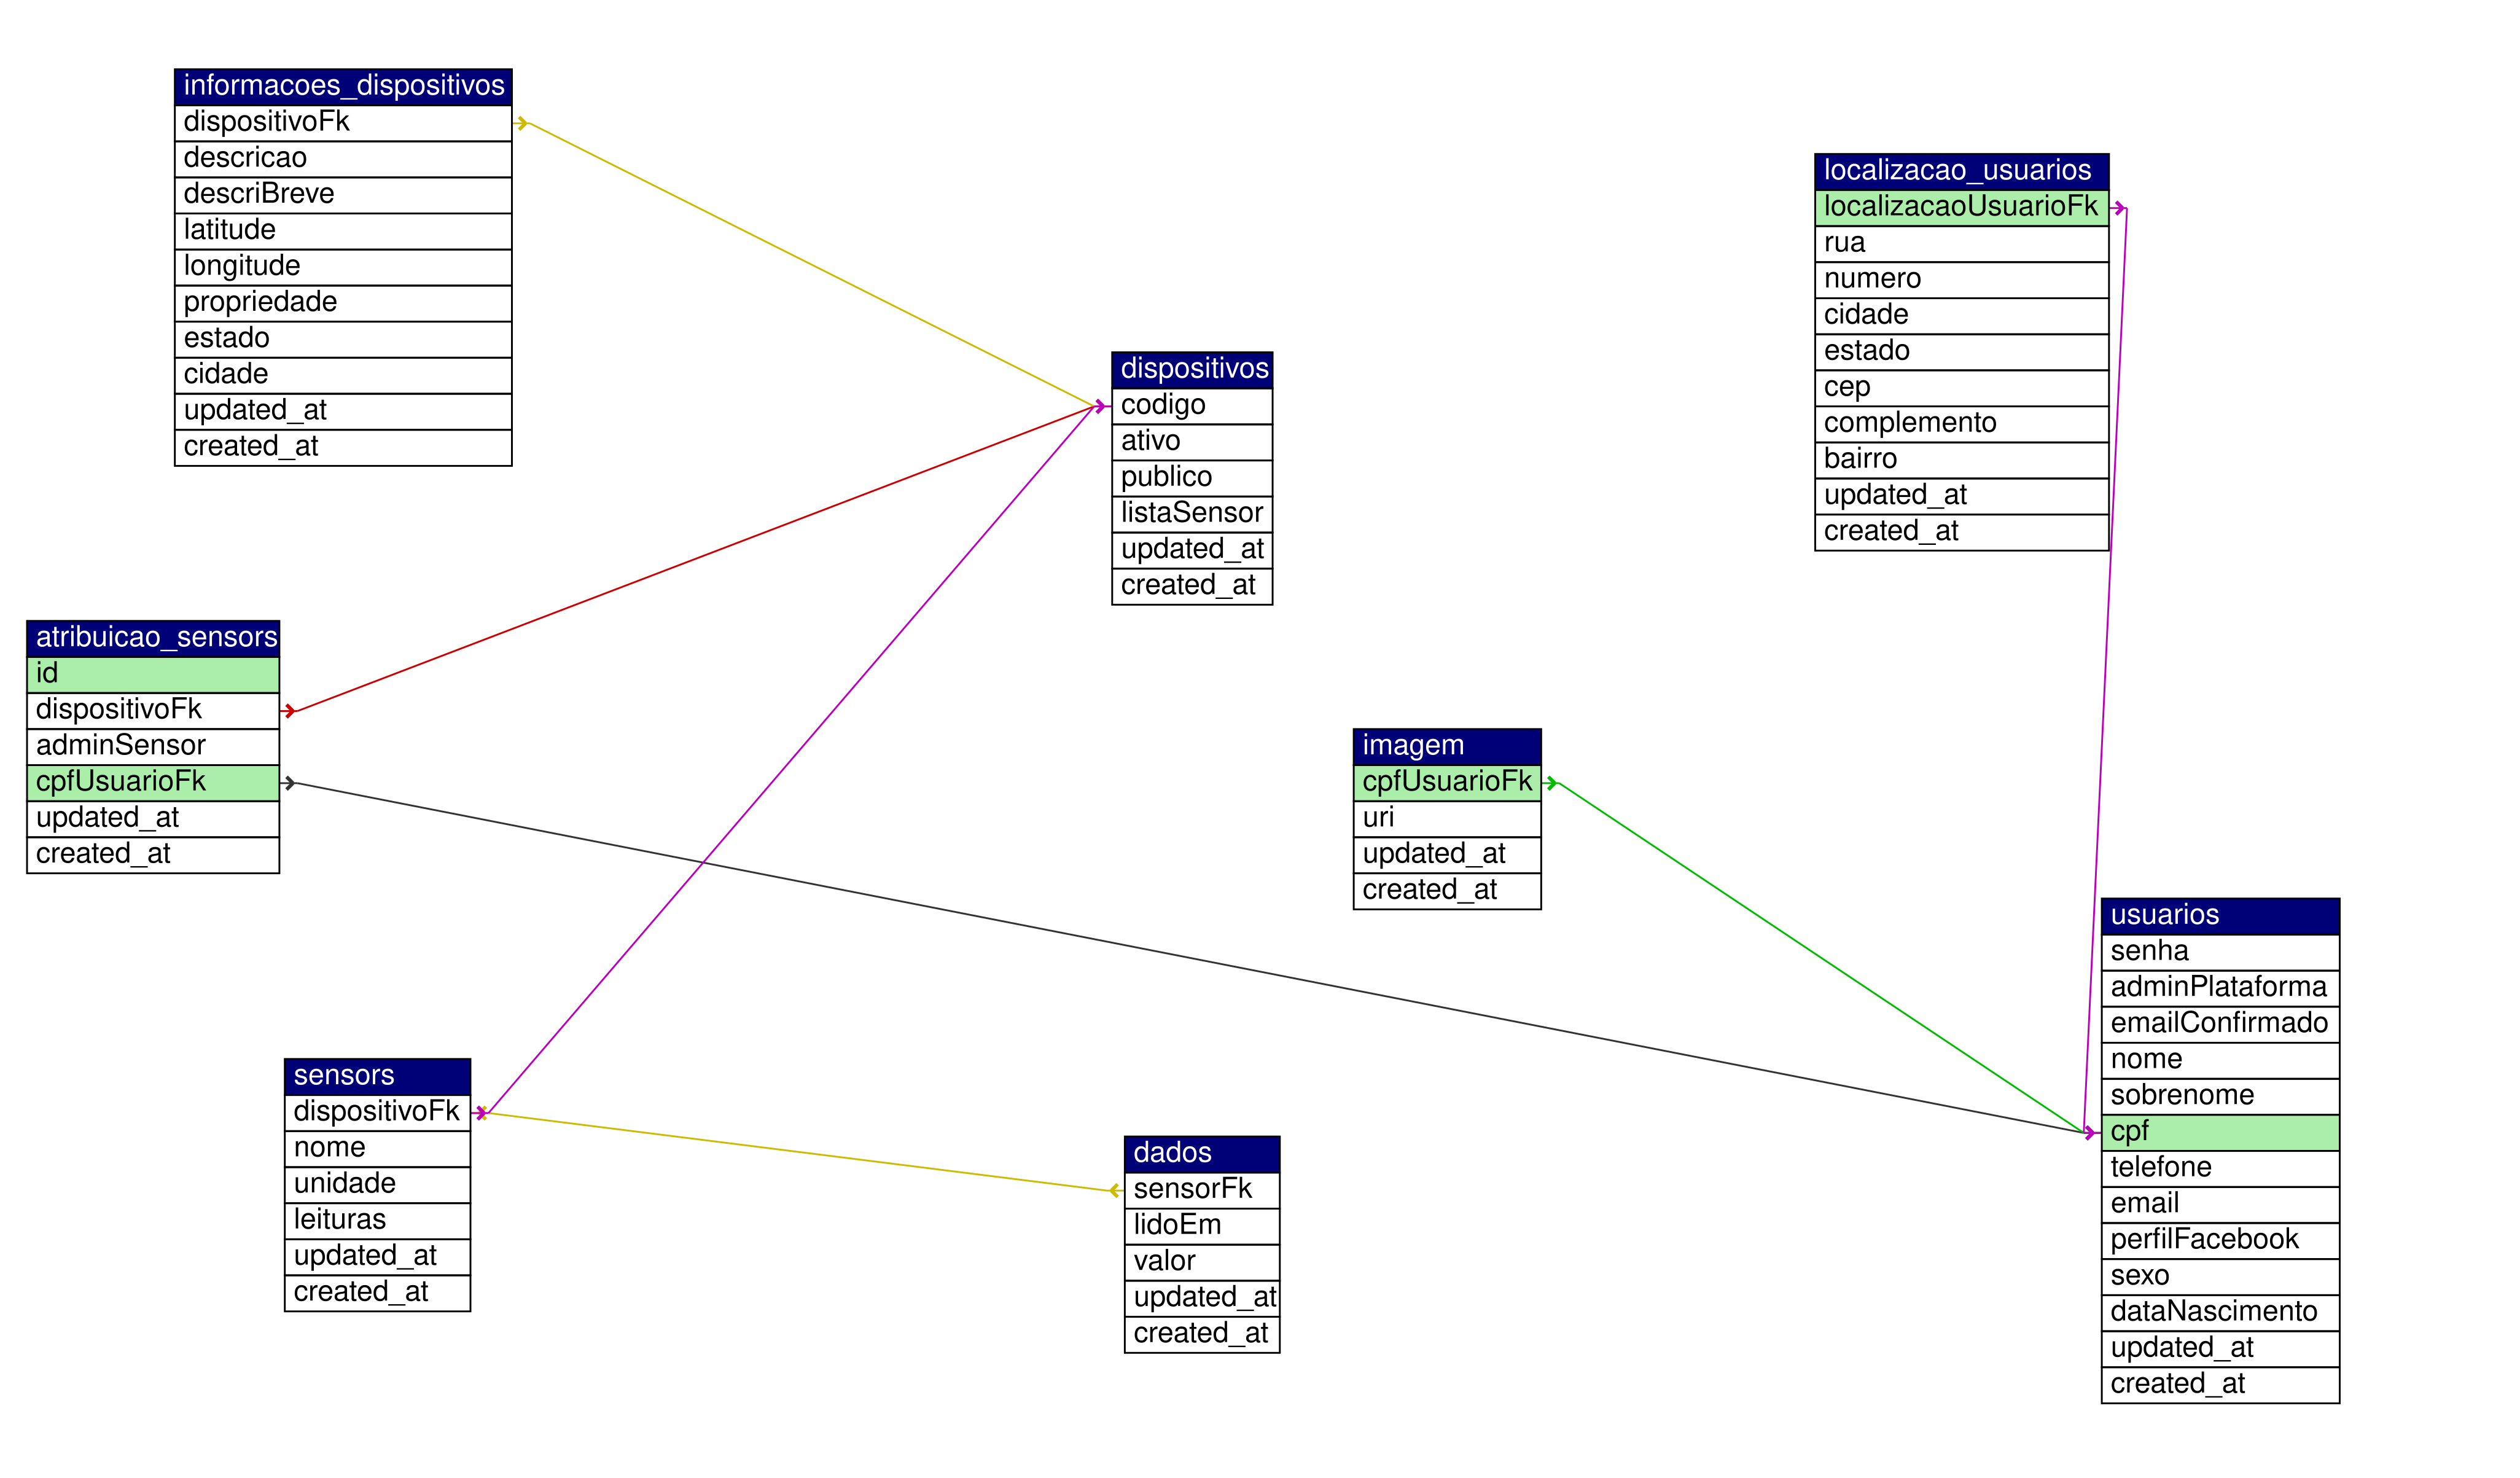
\includegraphics[scale=.5]{assets/app_nosconectadosfk.png}
  \caption{Banco de dados da plataforma utilizando o PHPMyAdmin}
  \label{bancodedados}
\end{figure}
\newpage

Nota-se que foi necessário a criação de diversas tabelas utilizando-se de chaves estrangeiras para estabelecer relacionamentos entre os dados armazenados, cada uma com seus respectivos atributos. A tabela \ref{tab:usuarios-structure} representa a tabela de usuários do banco, que conta com informações como a senha, um atributo chamado admin, que é responsável por definir se um usuário é comum ou um administrador. Nessa mesma tabela temos o  cpf como chave primária, há também a flag emailConfirmado, que indica se o email do usuário foi confirmado ou não, além do nome completo, telefone, email, perfil do Facebook, gênero, data de nascimento e os timestamps updated\_at e created\_at. Além disso, é importante ressaltar que o atributo "email"\space na tabela está em negrito, indicando que é um campo único.

%
% Estrutura: usuarios
%
\begin{longtable}{|l|c|c|c|l|l|}
\caption{Estrutura da tabela usuarios} \label{tab:usuarios-structure} \\
\hline \multicolumn{1}{|c|}{\textbf{Coluna}} & \multicolumn{1}{|c|}{\textbf{Tipo}} & \multicolumn{1}{|c|}{\textbf{Nulo}} & \multicolumn{1}{|c|}{\textbf{Padrão}} & \multicolumn{1}{|c|}{\textbf{Links para}} & \multicolumn{1}{|c|}{\textbf{MIME}} \\ \hline \hline
\endfirsthead
\caption{Estrutura da tabela usuarios (continuação)} \\
\hline \multicolumn{1}{|c|}{\textbf{Coluna}} & \multicolumn{1}{|c|}{\textbf{Tipo}} & \multicolumn{1}{|c|}{\textbf{Nulo}} & \multicolumn{1}{|c|}{\textbf{Padrão}} & \multicolumn{1}{|c|}{\textbf{Links para}} & \multicolumn{1}{|c|}{\textbf{MIME}} \\ \hline \hline \endhead \endfoot
senha & varchar(200) & Não &  &  &  \\ \hline
adminPlataforma & tinyint(1) & Não & 0 &  &  \\ \hline
emailConfirmado & tinyint(1) & Não & 0 &  &  \\ \hline
nome & varchar(30) & Não &  &  &  \\ \hline
sobrenome & varchar(30) & Não &  &  &  \\ \hline
\textbf{\textit{cpf}} & int(11) & Não &  &  &  \\ \hline
telefone & char(11) & Não &  &  &  \\ \hline
\textbf{email} & varchar(30) & Não &  &  &  \\ \hline
perfilFacebook & varchar(100) & Sim & NULL &  &  \\ \hline
sexo & char(1) & Não &  &  &  \\ \hline
dataNascimento & date & Sim & NULL &  &  \\ \hline
updated\_at & varchar(20) & Sim & NULL &  &  \\ \hline
created\_at & varchar(20) & Sim & NULL &  &  \\ \hline
\end{longtable}


A tabela imagem, vista na tabela \ref{tab:imagem-structure}, é responsável por armazenar a foto de perfil dos usuários, com atributos como o uri, cpfUsuarioFk (uma chave estrangeira que referencia o cpf da tabela de usuários), uri que é um tipo de dado do tipo MIME que representa o armazenamento de dados do tipo de arquivos, indicando que armazena a foto de perfil do usuário e os timestamps updated\_at e created\_at. Dessa forma, é possível notar que o atributo cpfUsuarioFk é tanto chave primária quanto chave estrangeira, essa abordagem é conhecida como "chave primária composta"\space ou "chave primária composta por chave estrangeira". 

%
% Estrutura: imagem
%
\begin{longtable}{|l|c|c|c|l|l|}
\caption{Estrutura da tabela imagem} \label{tab:imagem-structure} \\
\hline \multicolumn{1}{|c|}{\textbf{Coluna}} & \multicolumn{1}{|c|}{\textbf{Tipo}} & \multicolumn{1}{|c|}{\textbf{Nulo}} & \multicolumn{1}{|c|}{\textbf{Padrão}} & \multicolumn{1}{|c|}{\textbf{Links para}} & \multicolumn{1}{|c|}{\textbf{MIME}} \\ \hline \hline
\endfirsthead
\caption{Estrutura da tabela imagem (continuação)} \\
\hline \multicolumn{1}{|c|}{\textbf{Coluna}} & \multicolumn{1}{|c|}{\textbf{Tipo}} & \multicolumn{1}{|c|}{\textbf{Nulo}} & \multicolumn{1}{|c|}{\textbf{Padrão}} & \multicolumn{1}{|c|}{\textbf{Links para}} & \multicolumn{1}{|c|}{\textbf{MIME}} \\ \hline \hline \endhead \endfoot
\textbf{\textit{cpfUsuarioFk}} & int(11) & Não &  & usuarios (cpf) & \\ \hline
uri & varchar(255) & Não &  &  & image \\ \hline
updated\_at & varchar(20) & Sim & NULL &  & \\ \hline
created\_at & varchar(20) & Sim & NULL &  & \\ \hline
\end{longtable}


A tabela de localização de usuários, apresentada na tabela \ref{tab:localizacao_usuarios-structure}, inclui informações como rua, número, cidade, estado, endereço postal, complemento, bairro, usuarioFk (também uma chave estrangeira que referencia o cpf da tabela de usuários) e os timestamps updated\_at e created\_at.\

%
% Estrutura: localizacao_usuarios
%
\begin{longtable}{|l|c|c|c|l|l|}
\caption{Estrutura da tabela localizacao\_usuarios} \label{tab:localizacao_usuarios-structure} \\
\hline \multicolumn{1}{|c|}{\textbf{Coluna}} & \multicolumn{1}{|c|}{\textbf{Tipo}} & \multicolumn{1}{|c|}{\textbf{Nulo}} & \multicolumn{1}{|c|}{\textbf{Padrão}} & \multicolumn{1}{|c|}{\textbf{Links para}} & \multicolumn{1}{|c|}{\textbf{MIME}} \\ \hline \hline
\endfirsthead
\caption{Estrutura da tabela localizacao\_usuarios (continuação)} \\
\hline \multicolumn{1}{|c|}{\textbf{Coluna}} & \multicolumn{1}{|c|}{\textbf{Tipo}} & \multicolumn{1}{|c|}{\textbf{Nulo}} & \multicolumn{1}{|c|}{\textbf{Padrão}} & \multicolumn{1}{|c|}{\textbf{Links para}} & \multicolumn{1}{|c|}{\textbf{MIME}} \\ \hline \hline \endhead \endfoot
\textbf{\textit{usuarioFk}} & int(11) & Não &  & usuarios (cpf) &  \\ \hline
rua & varchar(60) & Não &  &  &  \\ \hline
numero & int(11) & Não &  &  &  \\ \hline
cidade & varchar(30) & Não &  &  &  \\ \hline
estado & varchar(30) & Não &  &  &  \\ \hline
cep & varchar(8) & Não &  &  &  \\ \hline
complemento & char(20) & Sim & NULL &  &  \\ \hline
bairro & varchar(30) & Não &  &  &  \\ \hline
updated\_at & varchar(20) & Sim & NULL &  &  \\ \hline
created\_at & varchar(20) & Sim & NULL &  &  \\ \hline
\end{longtable}


A tabela de sensores é um componente fundamental do banco de dados da plataforma, cuja estrutura pode ser vista na Tabela \ref{tab:sensors-structure}. Nela, são armazenadas informações essenciais como o nome do sensor, a unidade e a sua chave primária composta. Além disso, a tabela inclui um atributo denominado leituras, que é definido como um objeto do tipo JSON e contém todos os dados do sensor em formato de chave e valor. Esse formato de armazenamento é uma característica fundamental da plataforma, pois garante sua adaptabilidade a diferentes tipos de sensores.

%
% Estrutura: sensors
%
\begin{longtable}{|l|c|c|c|l|l|}
\caption{Estrutura da tabela sensors} \label{tab:sensors-structure} \\
\hline \multicolumn{1}{|c|}{\textbf{Coluna}} & \multicolumn{1}{|c|}{\textbf{Tipo}} & \multicolumn{1}{|c|}{\textbf{Nulo}} & \multicolumn{1}{|c|}{\textbf{Padrão}} & \multicolumn{1}{|c|}{\textbf{Links para}} & \multicolumn{1}{|c|}{\textbf{MIME}} \\ \hline \hline
\endfirsthead
\caption{Estrutura da tabela sensors (continuação)} \\
\hline \multicolumn{1}{|c|}{\textbf{Coluna}} & \multicolumn{1}{|c|}{\textbf{Tipo}} & \multicolumn{1}{|c|}{\textbf{Nulo}} & \multicolumn{1}{|c|}{\textbf{Padrão}} & \multicolumn{1}{|c|}{\textbf{Links para}} & \multicolumn{1}{|c|}{\textbf{MIME}} \\ \hline \hline \endhead \endfoot
\textbf{\textit{dispositivoFk}} & binary(16) & Não &  & dispositivos (codigo) &  \\ \hline
nome & varchar(30) & Não &  &  &  \\ \hline
unidade & varchar(50) & Não &  &  &  \\ \hline
leituras & JSON & Sim & NULL &  &  \\ \hline
updated\_at & varchar(20) & Sim & NULL &  &  \\ \hline
created\_at & varchar(20) & Sim & NULL &  &  \\ \hline
\end{longtable}

Há também as informações dos dispositivos, que contém uma breve descrição e uma descrição mais longa, latitude e longitude, nome da propriedade, estado e cidade. Essa tabela conta ainda com o atributo dispositivoFk, uma chave primária composta que referencia o codigo da tabela de dispositivos.

%
% Estrutura: informacoes_dispositivos
%
\begin{longtable}{|l|c|c|c|l|l|}
\caption{Estrutura da tabela informacoes\_dispositivos} \label{tab:informacoes_dispositivos-structure} \\
\hline \multicolumn{1}{|c|}{\textbf{Coluna}} & \multicolumn{1}{|c|}{\textbf{Tipo}} & \multicolumn{1}{|c|}{\textbf{Nulo}} & \multicolumn{1}{|c|}{\textbf{Padrão}} & \multicolumn{1}{|c|}{\textbf{Links para}} & \multicolumn{1}{|c|}{\textbf{MIME}} \\ \hline \hline
\endfirsthead
\caption{Estrutura da tabela informacoes\_dispositivos (continuação)} \\
\hline \multicolumn{1}{|c|}{\textbf{Coluna}} & \multicolumn{1}{|c|}{\textbf{Tipo}} & \multicolumn{1}{|c|}{\textbf{Nulo}} & \multicolumn{1}{|c|}{\textbf{Padrão}} & \multicolumn{1}{|c|}{\textbf{Links para}} & \multicolumn{1}{|c|}{\textbf{MIME}} \\ \hline \hline \endhead \endfoot
\textbf{dispositivoFk} & binary(16) & Não &  & dispositivos (codigo) &  \\ \hline
descricao & varchar(300) & Sim & NULL &  &  \\ \hline
descriBreve & varchar(150) & Não &  &  &  \\ \hline
latitude & decimal(10,8) & Sim & NULL &  &  \\ \hline
longitude & decimal(11,8) & Sim & NULL &  &  \\ \hline
propriedade & varchar(30) & Não &  &  &  \\ \hline
estado & varchar(30) & Não &  &  &  \\ \hline
cidade & varchar(30) & Não &  &  &  \\ \hline
updated\_at & varchar(20) & Sim & NULL &  &  \\ \hline
created\_at & varchar(20) & Sim & NULL &  &  \\ \hline
\end{longtable}


Ainda há a tabela de dispositivos, que armazena uma flag denominada "ativo"\space que indica se o sensor está ativo, inativo ou pendente, uma flag "publico", que indica se o sensor é público ou privado, a lista de sensores que estão incorporados neste dispositivo, e os seus determinados timestamps.
%
% Estrutura: dispositivos
%
\begin{longtable}{|l|c|c|c|l|l|}
\caption{Estrutura da tabela dispositivos} \label{tab:dispositivos-structure} \\
\hline \multicolumn{1}{|c|}{\textbf{Coluna}} & \multicolumn{1}{|c|}{\textbf{Tipo}} & \multicolumn{1}{|c|}{\textbf{Nulo}} & \multicolumn{1}{|c|}{\textbf{Padrão}} & \multicolumn{1}{|c|}{\textbf{Links para}} & \multicolumn{1}{|c|}{\textbf{MIME}} \\ \hline \hline
\endfirsthead
\caption{Estrutura da tabela dispositivos (continuação)} \\ 
\hline \multicolumn{1}{|c|}{\textbf{Coluna}} & \multicolumn{1}{|c|}{\textbf{Tipo}} & \multicolumn{1}{|c|}{\textbf{Nulo}} & \multicolumn{1}{|c|}{\textbf{Padrão}} & \multicolumn{1}{|c|}{\textbf{Links para}} & \multicolumn{1}{|c|}{\textbf{MIME}} \\ \hline \hline \endhead \endfoot
\textbf{\textit{codigo}} & binary(16) & Não &  &  &  \\ \hline
ativo & tinyint(2) & Não & 0 &  &  \\ \hline
publico & tinyint(1) & Não & 0 &  &  \\ \hline
listaSensor & JSON & Sim & NULL &  &  \\ \hline
updated\_at & varchar(20) & Sim & NULL &  &  \\ \hline
created\_at & varchar(20) & Sim & NULL &  &  \\ \hline
\end{longtable}

 
Por fim, há a tabela de atribuição dos sensores, responsável por armazenar as atribuições dos usuários aos seus respectivos sensores. Nessa tabela, há o id, dispositivoFk (uma chave estrangeira que referencia o codigo da tabela de dispositivos), flag adminSensor, que indica se um usuário é administrador, patrocinador ou visualizador da plataforma, com valores 2, 1 e 0, respectivamente, o atributo cpfUsuarioFk (uma chave estrangeira que referencia o cpf na tabela de usuários) e os timestamps.


% Estrutura: atribuicao_sensors
%
\begin{longtable}{|l|c|c|c|l|l|}
\caption{Estrutura da tabela atribuicao\_sensors} \label{tab:atribuicao_sensors-structure} \\
\hline \multicolumn{1}{|c|}{\textbf{Coluna}} & \multicolumn{1}{|c|}{\textbf{Tipo}} & \multicolumn{1}{|c|}{\textbf{Nulo}} & \multicolumn{1}{|c|}{\textbf{Padrão}} & \multicolumn{1}{|c|}{\textbf{Links para}} & \multicolumn{1}{|c|}{\textbf{MIME}} \\ \hline \hline
\endfirsthead
\caption{Estrutura da tabela atribuicao\_sensors (continuação)} \\
\hline \multicolumn{1}{|c|}{\textbf{Coluna}} & \multicolumn{1}{|c|}{\textbf{Tipo}} & \multicolumn{1}{|c|}{\textbf{Nulo}} & \multicolumn{1}{|c|}{\textbf{Padrão}} & \multicolumn{1}{|c|}{\textbf{Links para}} & \multicolumn{1}{|c|}{\textbf{MIME}} \\ \hline \hline \endhead \endfoot
\textbf{\textit{id}} & int(11) & Não &  &  &  \\ \hline
\textbf{\textit{dispositivoFk}} & binary(16) & Não &  & dispositivos (codigo) &  \\ \hline
adminSensor & tinyint(2) & Não & 2 &  &  \\ \hline
\textbf{\textit{cpfUsuarioFk}} & int(11) & Não &  & usuarios (cpf) &  \\ \hline
updated\_at & char(20) & Sim & NULL &  &  \\ \hline
created\_at & char(20) & Sim & NULL &  &  \\ \hline
\end{longtable}



 E, como não poderia faltar, há ainda a tabela de dados, responsável por armazenar os dados históricos dos sensores, com os mesmos atributos da tabela de sensores e o atributo sensorFk  representando a chave estrangeira que referencia a chave primária da tabela de sensores. Uma diferença importante a ser destacada é o uso de UUIDs (identificadores únicos universais) como chaves primárias na tabela de dados, em vez de utilizar inteiros. Os UUIDs são identificadores de 128 bits que têm uma probabilidade extremamente baixa de se repetirem, mesmo em conjuntos de dados grandes e são armazenados no formato de Binary(16). Essa escolha garante a unicidade das chaves primárias sem a necessidade de serem inteiros. Na tabela de dados, sempre que um novo dado é enviado para a tabela de sensores, uma cópia desse dado é armazenada na tabela de dados como uma nova linha, enquanto na tabela de sensores o dado é sobrescrito.

Essa abordagem permite preservar o histórico completo dos dados recebidos pelos sensores ao longo do tempo, garantindo a rastreabilidade e a capacidade de análise retrospectiva. Ao utilizar UUIDs como chaves primárias na tabela de dados, a integridade dos dados é mantida e evita-se conflitos de sobreposição entre as diferentes entradas de dados dos sensores.
%
% Estrutura: dados
%
\begin{longtable}{|l|c|c|c|l|l|}
\caption{Estrutura da tabela dados} \label{tab:dados-structure} \\
\hline \multicolumn{1}{|c|}{\textbf{Coluna}} & \multicolumn{1}{|c|}{\textbf{Tipo}} & \multicolumn{1}{|c|}{\textbf{Nulo}} & \multicolumn{1}{|c|}{\textbf{Padrão}} & \multicolumn{1}{|c|}{\textbf{Links para}} & \multicolumn{1}{|c|}{\textbf{MIME}} \\ \hline \hline
\endfirsthead
\caption{Estrutura da tabela dados (continuação)} \\ 
\hline \multicolumn{1}{|c|}{\textbf{Coluna}} & \multicolumn{1}{|c|}{\textbf{Tipo}} & \multicolumn{1}{|c|}{\textbf{Nulo}} & \multicolumn{1}{|c|}{\textbf{Padrão}} & \multicolumn{1}{|c|}{\textbf{Links para}} & \multicolumn{1}{|c|}{\textbf{MIME}} \\ \hline \hline \endhead \endfoot
\textbf{\textit{sensorFk}} & binary(16) & Não &  & sensors (dispositivoFk) &  \\ \hline
lidoEm & varchar(30) & Não &  &  &  \\ \hline
valor & float & Sim & NULL &  &  \\ \hline
updated\_at & varchar(20) & Sim & NULL &  &  \\ \hline
created\_at & varchar(20) & Sim & NULL &  &  \\ \hline
\end{longtable}


Em conclusão, a seção de desenvolvimento do banco de dados foi fundamentada no diagrama de entidade relacionamento e no modelo lógico do banco de dados elaborados durante a etapa de modelagem, como descrito na seção 3.2. Esses diagramas serviram como base para o desenvolvimento do banco de dados, permitindo uma visualização clara das tabelas e suas relações que foram desenvolvidas nesta etapa. Através da figura gerada pelo PHPMyAdmin, apresentamos uma visão detalhada dos tipos de dados, atributos, chaves primárias e estrangeiras de cada tabela. Essa abordagem meticulosa garantiu um desenvolvimento consistente e otimizado do banco de dados, com a devida atenção aos detalhes. Com isso, o banco de dados está bem estruturado e preparado para atender às necessidades do sistema, proporcionando um sólido alicerce para a próxima fase do projeto.


\subsection{Autenticação}
\label{sec:autenticacao}
Para os usuários, o processo de autenticação é baseado em tokens JWT (JSON Web Tokens) e é realizado através de um formulário de login no front-end. Quando o usuário faz login na plataforma, os dados do formulário são enviados para a API da plataforma em um objeto JSON. Em seguida, o back-end realiza a autenticação do usuário, verificando se as credenciais de login são válidas. Se o login for bem sucedido, um token JWT é gerado e enviado de volta para o front-end. Esse token é então armazenado na session storage do navegador e é enviado no cabeçalho de cada requisição feita pelo usuário, no campo "Authorization" \space do protocolo HTTP.

Na figura \ref{jwtuser} é possível ver como é feito o fluxo de autenticação de usuários na plataforma utilizando JWT. A partir da figura é possível notar que esse tipo de autenticação se torna eficiente justamente por evitar a necessidade de manter um estado de sessão no servidor e elimina a necessidade de enviar credenciais de login em cada requisição.

\begin{figure}[htbp]
  \centering 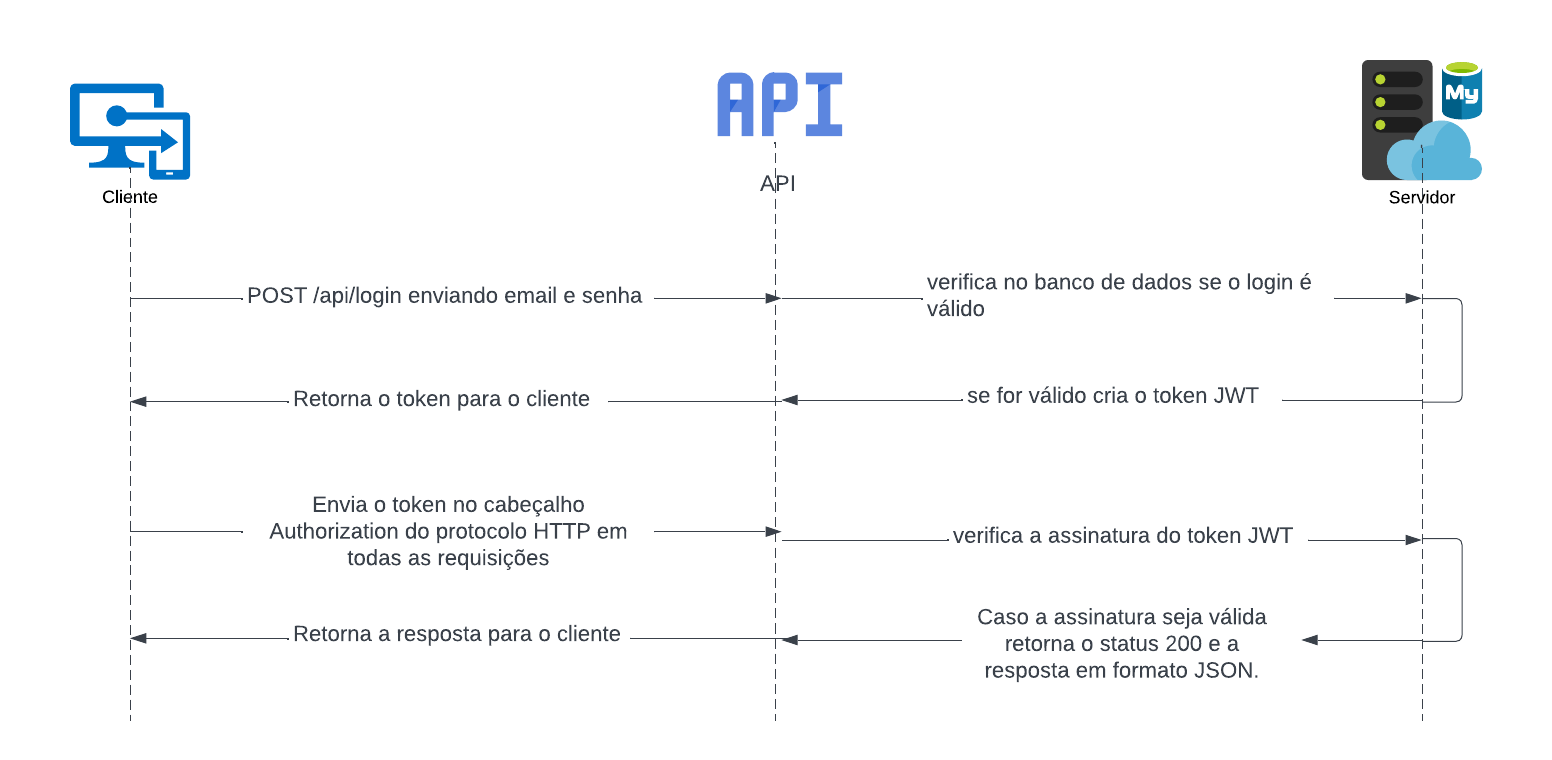
\includegraphics[scale=.5]{assets/jwtauth.png}
  \caption{Fluxo de autenticação de usuários}
  \label{jwtuser}
\end{figure}


Também é utilizado o Vuex para gerenciar se o usuário está logado ou não. Quando o usuário faz login na plataforma, o Vuex é acionado para armazenar o estado de login. Isso é feito criando um objeto de estado no Vuex, que armazena a informação de que o usuário está autenticado. Em seguida, essa informação é compartilhada com todos os componentes da aplicação que precisam dela, tornando o estado do login disponível em toda a aplicação.

Quando o usuário sai da plataforma, o estado do Vuex é atualizado para indicar que ele não está mais autenticado. Novamente, essa informação é compartilhada com todos os componentes da aplicação que precisam dela. Além disso, o Vuex é usado para gerenciar outros aspectos do estado da aplicação, como a configuração de sensores, a exibição de gráficos de dados, etc.

Além disso, há um tipo de autenticação para os sensores que enviam dados para a API da plataforma. Para que a API aceite dados dos sensores, é necessário que os sensores enviem um token único no campo de cada requisição. Esse token também é baseado em JWT, gerado para cada sensor e utilizado para autenticar o sensor junto à plataforma. Essa autenticação é realizada antes que os dados enviados pelo sensor sejam armazenados na plataforma.

Na figura \ref{jwtapi} é possível visualizar o processo de autenticação dos sensores. Ao criar um sensor na plataforma, é possível gerar um token JWT exclusivo na seção de atribuição do sensor. Esse token é utilizado para autenticação e pode ser adicionado diretamente no firmware do sensor, e uma vez que esteja nele, não será mais necessário gerar um novo token a cada requisição, pois o mesmo será enviado automaticamente no cabeçalho "Authorization" \space do protocolo HTTP em todas as solicitações enviadas. Essa abordagem de autenticação fornece um alto nível de segurança e eficiência no processo de comunicação entre o sensor e a plataforma.
\begin{figure}[htbp]
  \centering 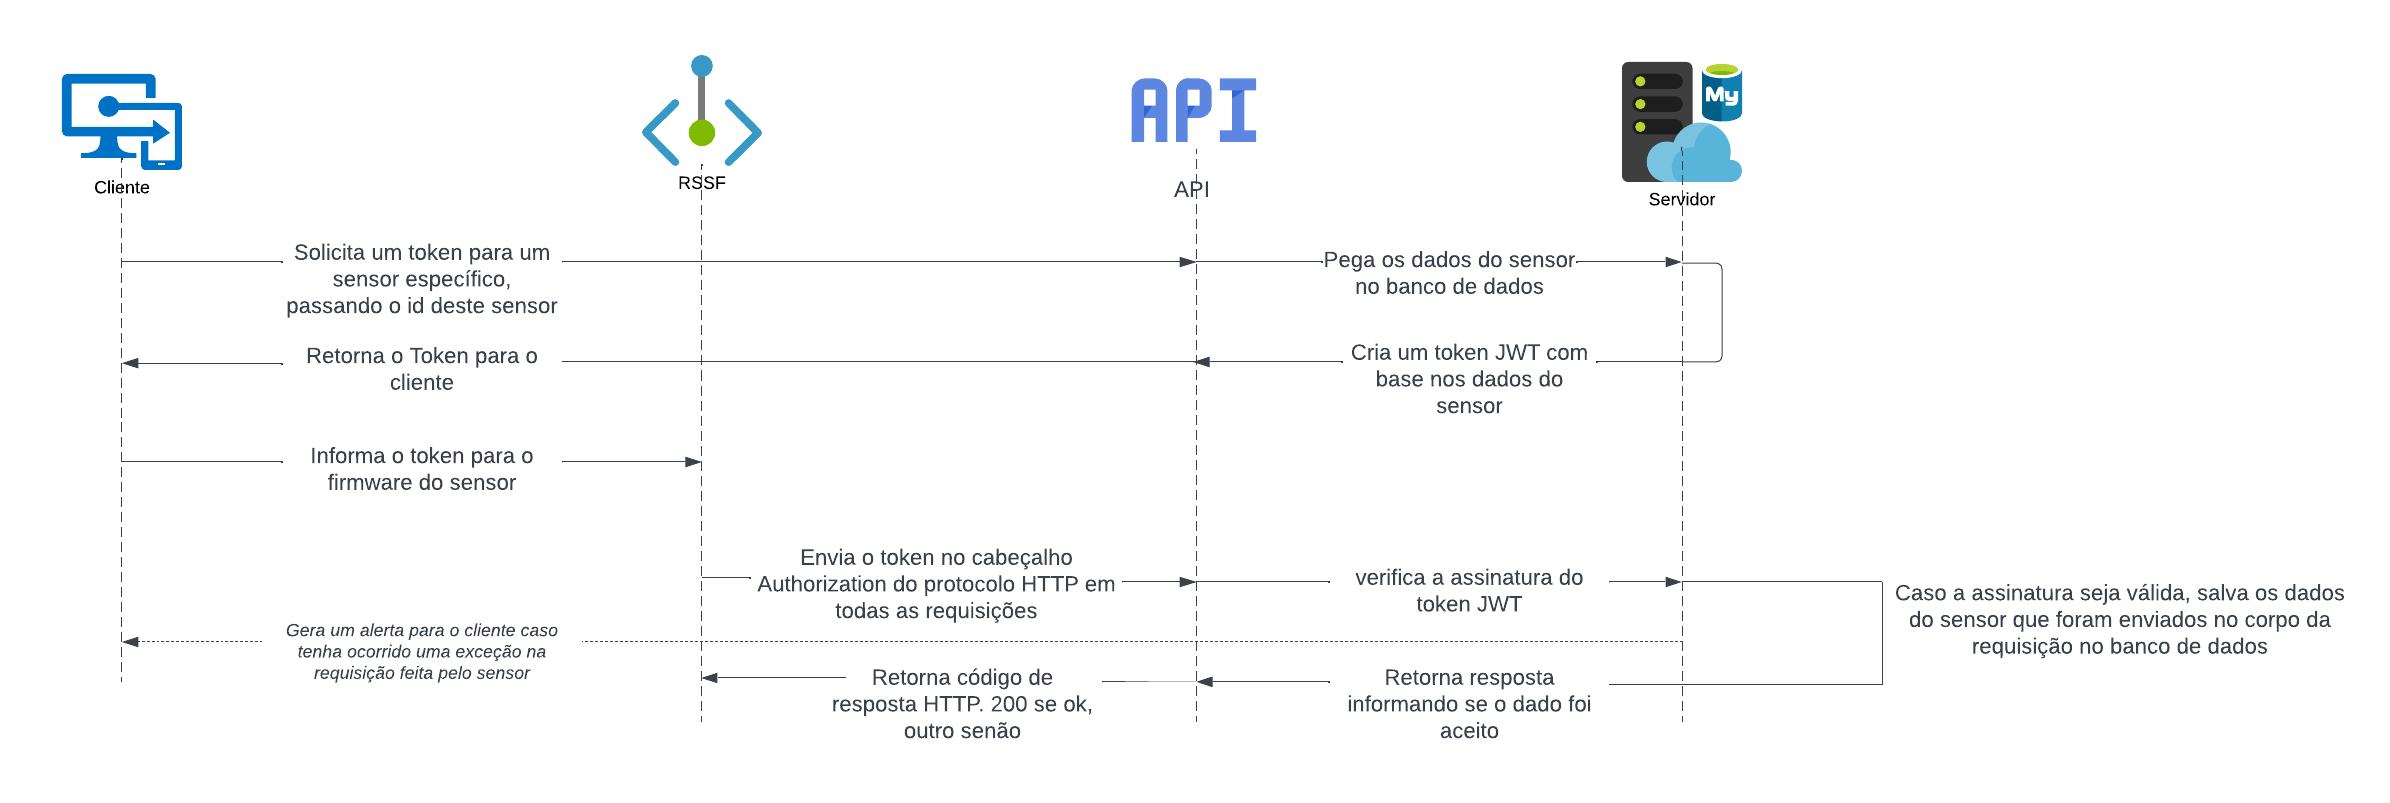
\includegraphics[scale=.4]{assets/jwtauthapi.png}
  \caption{Fluxo de autenticação de sensores}
  \label{jwtapi}
\end{figure}

Também existe uma preocupação em restringir o acesso a determinadas rotas da plataforma caso o usuário não esteja autenticado ou não tenha acesso autorizado. Para isso utilizamos um middleware no front-end, em específico o middlewareAuth do Vue.js \cite{vue:2014}, que funciona através da verificação da autenticação do usuário e do acesso autorizado às páginas, e redireciona o usuário para outras páginas caso ele não atenda a essas condições. 

O middlewareAuth é uma função que pode ser definida para rodar antes de cada navegação de rota. Essa função é responsável por verificar se o usuário está autenticado e se tem acesso autorizado à página que ele está tentando acessar. Caso o usuário não esteja autenticado ou não tenha acesso autorizado, o middlewareAuth pode redirecioná-lo para outra página, como a página de login ou a página inicial da plataforma. Para isso, é necessário a biblioteca Vue Router do Vue.js \cite{vue:2014}, pois para a sua implementação é necessário definir a função que verifica a autenticação do usuário e o acesso autorizado às páginas. Essa função pode ser chamada antes de cada navegação de rota, usando a função \textit{"beforeEach"} do Vue Router. A função \textit{"beforeEach"} recebe o objeto \textit{"to"} que representa a rota que o usuário está tentando acessar, e o objeto \textit{"from"} que representa a rota atual.

O pseudo-código apresentado abaixo exemplifica como a função middlewareAuth pode ser implementada, utilizando a biblioteca Vue Router:\\

\begin{algorithm}[H]
\SetAlgoLined
\KwIn{Vue Router}
\KwOut{Redirecionamento para outra página}
\SetKwProg{Fn}{Function}{:}{}
\Fn{middlewareAuth()}{
\If{usuário não está autenticado ou não tem acesso autorizado à página}{
redirecionar usuário para outra página (como a página de login ou a página inicial da plataforma);
}
}

VueRouter.beforeEach((to, from, next) => {
middlewareAuth();
next();
})
\caption{Pseudo-código da função middlewareAuth}
\end{algorithm}
\hfill\break


Em suma, neste capítulo foram apresentados os diferentes aspectos da autenticação utilizados na plataforma, incluindo a autenticação baseada em tokens JWT para os usuários e sensores, a utilização do Vuex para gerenciar o estado de login do usuário, a autenticação dos sensores que enviam dados para a API da plataforma, e o uso do middlewareAuth do Vue.js \cite{vue:2014} para restringir o acesso a rotas não autorizadas. É importante notar que esses mecanismos de autenticação são essenciais para garantir a segurança e a privacidade dos usuários da plataforma, além de manter a integridade dos dados coletados pelos sensores. A implementação desses mecanismos também demonstra o compromisso em desenvolver a plataforma visando a máxima qualidade e confiabilidade possível.
\subsection{Dashboards}
A subseção de dashboards é um componente fundamental da plataforma, sendo descrito como um requisito funcional chave. Embora esse tipo de funcionalidade geralmente seja considerado um requisito não-funcional, aqui ela é essencial, pois permite que os usuários visualizem séries históricas geradas pelos sensores em tempo real. Esses gráficos fornecem uma visão geral dos dados coletados pelos sensores e a plataforma oferece aos usuários a possibilidade de personalizar a visualização de acordo com suas necessidades específicas. Os usuários podem manipular os gráficos, selecionar quais seções desejam ver e fazer alterações nos gráficos para ver como os dados históricos foram afetados. Essa flexibilidade dá aos usuários um maior controle sobre os dados coletados e ajuda na tomada de decisões informadas.

Para a plotagem dos gráficos, foi utilizada a biblioteca Apexcharts.js \cite{ApexCharts:2022} do Vue.js \cite{vue:2014}, que é uma biblioteca de código aberto para a criação gráficos interativos. E para a geração dos gráficos, foram utilizados os dados históricos gerados pelos sensores. Isso significa que a cada vez que um sensor envia dados para a plataforma, esses dados são colocados no banco de dados, especificamente na tabela "dados". Essas informações contêm o ID do sensor que está enviando os dados, o readAt que indica quando esses dados foram lidos e as informações dos sensores, que podem ser temperatura do solo, pluviômetro, temperatura do ar, entre outros.

Por padrão, a plataforma tem três gráficos principais: o gráfico de pluviômetro, que é mostrado em formato de gráfico de barra; o gráfico de temperatura, que é mostrado em gráfico de linha; e o gráfico referente à atmosfera, que é mostrado em gráfico de radar. Esses gráficos são desenvolvidos com o objetivo de ajudar os usuários na tomada de decisão, apresentando informações relevantes de forma clara e acessível. Além dos gráficos padrões, a plataforma também permite a criação de gráficos personalizados, de acordo com as necessidades do usuário.

Em resumo, os dashboards apresentados na plataforma são uma ferramenta crucial para visualizar e analisar as informações coletadas pelos sensores. Eles permitem que os usuários tomem decisões informadas com base nos dados coletados.

\subsection{Controle de administração}
Na seção de controle de administração da plataforma existem dois tipos de administração: a administração geral da plataforma e a administração dos sensores. No caso da administração geral da plataforma, o usuário administrador tem acesso total à plataforma, incluindo um painel de administração que permite remover usuários da plataforma e alterar qualquer informação referente a qualquer sensor ou usuário que não seja um administrador. O usuário comum, por sua vez, tem acesso limitado à plataforma, podendo apenas gerenciar as suas próprias informações e seus próprios sensores que podem ter sido criados por ele ou referenciados à ele por outros usuários.

Contudo, para o usuário comum, o controle de administração dos sensores é uma das partes mais importantes da plataforma. Ele permite que os usuários possam gerenciar seus próprios sensores e controlar quem tem acesso às informações coletadas. Dessa forma, quando um usuário cria um sensor, automaticamente ele se torna o administrador daquele sensor. Isso significa que ele tem acesso total às informações coletadas por aquele sensor, bem como às configurações e ajustes do sensor.

O administrador do sensor pode adicionar outros usuários como administradores, patrocinadores ou visualizadores para aquele sensor. Um administrador de um sensor possui as mesmas funções que o usuário que criou o sensor. Isso significa que ele pode modificar as configurações do sensor, acessar as informações coletadas e gerenciar os usuários do sensor.

Um patrocinador é um usuário secundário que pode ser adicionado pelo administrador do sensor. Um patrocinador não pode adicionar ou remover outros usuários do sensor, mas pode modificar as informações do sensor, como sua localização geográfica ou outras configurações. Isso pode ser útil para sensores que precisam ser atualizados regularmente, mas não devem ser acessados por todos os usuários da plataforma.

Já um visualizador é um usuário que pode apenas visualizar as informações coletadas pelo sensor. Ele não pode modificar as configurações do sensor ou adicionar ou remover outros usuários. Os visualizadores são úteis para sensores privados que devem ser acessados apenas por usuários específicos.

O controle de administração dos sensores é importante para garantir a segurança das informações coletadas e para permitir que os usuários possam gerenciar seus próprios sensores de forma eficiente. Ele permite que os usuários controlem quem tem acesso às informações e quem pode modificar as suas configurações, tornando a plataforma mais segura e confiável para todos os usuários.
\subsection{Camadas de segurança}
A segurança é um aspecto crítico em qualquer aplicação Web, especialmente quando se trata de plataformas que lidam com dados sensíveis. Nesta seção, descreveremos as camadas de segurança que foram adicionadas ao nosso sistema para garantir a integridade, a confidencialidade e a disponibilidade dos dados.

Para o back-end, utilizamos o PDO \cite{PDO:2022} para lidar com a comunicação com o banco de dados MySQL \cite{mysql:2022}. O PDO é uma extensão do PHP \cite{PHP:2022} que fornece uma interface de acesso a banco de dados consistente e segura. Ele ajuda a evitar a injeção de SQL, que é uma técnica comum de ataque cibernético que aproveita vulnerabilidades de entrada de dados maliciosos em consultas SQL para executar comandos mal-intencionados.

A escolha do framework no back-end foi outra medida de segurança importante, pois o Slim \cite{slim:2023} é um framework leve e flexível que ajuda a proteger nossas rotas de acesso a dados de forma segura. Além disso, o Slim também possui uma camada de segurança embutida que ajuda a evitar vulnerabilidades comuns, como XSS e CSRF.

No front-end, a escolha do framework também ajudou a constituir uma plataforma mais confiável, pois a progressividade do Vue.js oferece uma camada de segurança para prevenir vulnerabilidades comuns em aplicações web, como a injeção de código. Ele também possui recursos de validação de entrada de dados, o que nos ajudou a garantir que os dados recebidos do usuário não sejam maliciosos.

Por fim, todas as informações confidenciais, como senhas e chaves de acesso, foram armazenadas de forma criptografada no banco de dados, utilizando técnicas de hashing e salting. Isso garante que, mesmo que um atacante tenha acesso aos dados armazenados, eles não possam ser facilmente decifrados.

Ao implementar essas camadas de segurança em nossas plataformas, garantimos que nossos dados e usuários estejam protegidos contra vulnerabilidades comuns em aplicações web. No entanto, é importante lembrar que a segurança é um processo contínuo e que novas ameaças surgem constantemente. Portanto, a manutenção e atualização contínua de nossas camadas de segurança descritas na seção \ref{sec:manutencao} é essencial para manter nossa plataforma segura.


\section{Testes}
\label{sec:testes}
A seção de testes é uma etapa fundamental no desenvolvimento de uma plataforma para garantir que todas as funcionalidades estão operando corretamente. Nesta seção serão descritas as etapas de teste da plataforma.

%Para realizar os testes no front-end da plataforma, foi utilizada a biblioteca Jest \cite{Jest:2023} para testes unitários e Cypress \cite{Cypress:2023} para testes de integração. Jest é uma biblioteca de testes de JavaScript criada pelo Facebook que oferece uma ampla gama de funcionalidades, incluindo a capacidade de testar código Vue.js. Já o Cypress é uma biblioteca de testes de front-end de última geração que permite testar aplicativos da Web modernos em vários navegadores.\\

%No back-end da plataforma, foi utilizado PHPUnit \cite{PHPUnit:2022} para testes unitários e o Postman \cite{Postman:2023} para testes de integração. PHPUnit é uma biblioteca de testes de unidade para PHP \cite{PHP:2022} que fornece um ambiente de teste completo e fácil de usar para a criação de testes de unidade em PHP. Já o Postman é uma ferramenta de testes de API que permite criar, testar e documentar solicitações de API com facilidade.\\

Os testes %de aceitação
foram conduzidos utilizando o PageSpeed Insights \cite{PageSpeedInsights:2023}, uma ferramenta amplamente reconhecida para avaliar o desempenho de sistemas web. Esses testes têm como objetivo verificar se o sistema atende aos requisitos e expectativas do usuário final, em relação à performance e velocidade de carregamento das páginas. Para garantir a máxima fidelidade dos resultados, os testes foram realizados na aplicação em produção, utilizando o servidor de hospedagem real, para simular as condições reais de uso. Dessa forma, foi possível avaliar o desempenho do carregamento das páginas em um ambiente de produção, garantindo que o sistema estivesse apto para atender às demandas dos usuários finais em termos de performance e velocidade.

%\subsection{Testes unitários}
%O principal objetivo dos testes unitários é detectar falhas de forma precoce, antes que possam se propagar e comprometer o funcionamento do sistema como um todo. Além disso, os testes unitários ajudam a manter a qualidade do código, aumentando a confiabilidade e a facilidade de manutenção do software. Fowler \cite{Fowler1999} afirma que a geração de testes unitários é um desafio, principalmente quando se trata de projetos complexos. No entanto, a realização desses testes é crucial para garantir a qualidade do software.\\

%Para a realização dos testes no back-end, foi utilizada a ferramenta PHPUnit \cite{PHPUnit:2022}, que é uma estrutura de teste unitário para PHP \cite{PHP:2022}. Com o PHPUnit, foram criados testes para verificar a funcionalidade dos controladores, modelos e funções do back-end.\\

%Para o front-end, foi utilizado a ferramenta Jest \cite{Jest:2023}, que é um framework de teste para JavaScript. Com essa ferramenta, foi possível criar testes para verificar a funcionalidade dos componentes Vue.js, como formulários e botões. De acordo com Beck \cite{Beck:2003:TDD:861319}, a utilização de ferramentas de automação de testes é importante para garantir a eficiência dos testes unitários. Com essas ferramentas, é possível realizar os testes de forma mais rápida e eficiente, além de permitir a execução de testes repetidamente sem a necessidade de intervenção humana.

%\subsubsection{Front-end}
%Utilizando os recursos da ferramenta Jest \cite{Jest:2023}, foram escritos testes para verificar se os componentes estavam sendo renderizados corretamente, bem como se os dados estavam sendo passados de forma adequada entre os componentes. Para isso, foram utilizados mocks de dados para simular diferentes situações.\\

%Também foram criados testes para verificar se as funcionalidades estavam funcionando corretamente. Para isso, foram criados casos de teste para verificar a validação de campos, a exibição de mensagens de erro e o redirecionamento para outras páginas. A utilização de testes de snapshot também foi uma importante abordagem para garantir que o layout do componente não foi alterado inadvertidamente.\\

%Além disso, foram realizados testes de integração com a API do back-end, utilizando mocks de chamadas HTTP para simular as respostas do servidor. Dessa forma, foi possível verificar se as requisições estavam sendo feitas corretamente e se os dados estavam sendo tratados da forma adequada no front-end. Com isso, foi possível garantir que o código estava funcionando corretamente e que novas funcionalidades ou modificações não iriam impactar negativamente na aplicação.\\

%Por fim, foi utilizado o recurso de "watch mode"\space do Jest para permitir que os testes sejam executados automaticamente sempre que houver mudanças no código do projeto. Isso permite uma abordagem de "desenvolvimento orientado a testes"\space (TDD), onde os testes são executados continuamente durante o desenvolvimento do projeto.
%\subsubsection{Back-end}
%Primeiramente, para utilizar a ferramenta do PHPUnit \cite{PHPUnit:2022} foi necessário configurar o ambiente para permitir a execução dos testes. Em seguida, foram escritos testes para cada função ou método da aplicação que necessitava de validação.\\

%Cada teste foi criado para verificar um cenário específico, com entradas e saídas conhecidas. Foram testados casos de sucesso e de falha, para garantir que a aplicação se comportasse corretamente em ambas as situações. Além disso, foram utilizados recursos como asserções para verificar se o comportamento da aplicação está de acordo com o esperado.\\

%Os testes foram organizados em grupos, de acordo com a funcionalidade que está sendo testada. Também foi criado um grupo de testes que verifica a integração entre diferentes partes da aplicação, como a comunicação entre o back-end e o banco de dados.\\

%Por fim, para garantir que os testes sejam executados regularmente, foi criado um script de automatização de testes. Esse script é executado sempre que há uma nova versão da aplicação ou quando há alguma mudança significativa no código-fonte. Com essa prática, é possível garantir que a aplicação permaneça funcionando corretamente mesmo após atualizações ou modificações no código.
%\subsection{Testes de integração}
%A realização de testes de integração é essencial para garantir o funcionamento adequado de um sistema de software como um todo, integrando as diferentes partes e identificando possíveis falhas de comunicação entre elas. Segundo Canfora \cite{Canfora:2009}, as composições de serviços podem mudar dinamicamente para atender a condições variadas, tornando crucial testar a interoperabilidade dos serviços por meio de testes de integração.\\

%Na visão de Humble \cite{humble2010continuous} os testes de integração são extremamente importantes para aplicações que conversam com diversos sistemas externos por meio de uma série de protocolos diferentes ou que consistem em uma série de módulos fracamente acoplados com interações complexas entre eles. Esses testes podem ser escritos da mesma forma que os testes de aceitação normais e, geralmente, devem ser executados em dois contextos: primeiro, com o sistema sob teste em execução contra os sistemas externos reais nos quais ele depende ou réplicas desses sistemas controlados pelo provedor de serviço e, segundo, contra um ambiente de teste que você cria como parte de sua base de código. \\

%No back-end, os testes de integração foi utilizada a ferramenta do Postman \cite{Postman:2023}, que permite a criação de testes que verificam o comportamento do sistema em relação às solicitações de API, desde a entrada de dados até a saída esperada. De acordo com Kaner \cite{kaner1999testing}, os testes de integração no back-end devem ser cuidadosamente planejados e executados para garantir a cobertura adequada de todos os fluxos do sistema, incluindo possíveis cenários de erro.\\

%Já no front-end, a realização de testes de integração foram feitos utilizando a ferramenta Cypress \cite{Cypress:2023}, que permite a simulação de interações do usuário com a interface do sistema. Para utiliar o cypress de maneira eficiente e prática, utilizamos o plugin que está disponível na plataforma onde hospedamos o sistema, o Netlify, nele é possível integrar o framework ao plugin, o que facilita bastante na hora de desenvolver os testes.\\

%Em ambos os casos, os testes de integração foram incluídos como parte integrante do processo de desenvolvimento de software, visando garantir a qualidade do produto final entregue ao usuário.
%\subsubsection{Front-end}
%A seção de testes de integração para o front-end utilizando a ferramenta Cypress foi elaborada com o objetivo de garantir que o comportamento do sistema esteja adequado em diferentes ambientes e dispositivos, proporcionando uma experiência satisfatória ao usuário final. Foram realizados testes em diversos cenários, incluindo diferentes navegadores e dispositivos móveis, para garantir que o sistema funcione corretamente em todos eles.\\

%Para realizar os testes, foram definidos cenários de uso, que envolvem as principais funcionalidades do sistema, como a autenticação do usuário, a navegação entre as páginas e o preenchimento de formulários. Além disso, foram criados testes para validar a apresentação de mensagens de erro e alertas ao usuário, para garantir que o sistema esteja fornecendo informações claras e precisas.\\

%Ao final da execução dos testes, foi possível identificar alguns problemas no comportamento do sistema em determinados cenários, como a apresentação de uma mensagem de erro não esperada no formulário de cadastro de usuários. Esses problemas foram corrigidos e os testes foram executados novamente, garantindo que o sistema esteja funcionando corretamente em todos os cenários definidos.\\

%Em resumo, a realização de testes em diferentes cenários e ambientes contribuiu para identificação de problemas e sua correção, reduzindo o risco de erros e retrabalho no processo de desenvolvimento da plataforma.
%\subsubsection{Back-end}
 %A seção de testes de integração foi uma etapa que demandou um tempo razoavelmente longo e foi cuidadosamente planejada para garantir a cobertura adequada de todos os fluxos do sistema, incluindo possíveis cenários de erro e interação com outros módulos. Inicialmente, foram criados testes que verificam a integração entre o banco de dados e as camadas do back-end responsáveis pela manipulação dos dados. Foram testados os principais fluxos de cadastro, edição e exclusão de registros, garantindo que todas as operações sejam realizadas de forma correta e consistente.\\

 %Em seguida foram realizados testes para simular possíveis falhas e erros do sistema, como a inserção de dados inválidos, a tentativa de acesso não autorizado e a sobrecarga do servidor. Desta forma, foi possível verificar que o sistema está preparado para lidar com essas situações de forma adequada, mantendo a integridade dos dados e a disponibilidade do sistema.\\

 %Dessa forma, com a utilização da ferramenta Postman \cite{Postman:2023} e a realização de testes de integração minuciosos, foi possível garantir a qualidade e a confiabilidade do sistema, evitando possíveis problemas e retrabalhos no futuro.

%\subsection{Testes de aceitação}
%\label{sec:testesaceitacao}
%Os testes de aceitação foram conduzidos utilizando o PageSpeed Insights \cite{PageSpeedInsights:2023}, com o intuito de verificar se a nossa plataforma atende aos requisitos e expectativas dos usuários finais. O objetivo desses testes foi avaliar a performance e a velocidade de carregamento das páginas da nossa plataforma. Utilizamos a aplicação em produção, em um ambiente real de hospedagem, para simular as condições reais de uso. Dessa forma, pudemos obter resultados mais precisos e relevantes para a experiência do usuário final.\\

O PageSpeed nos permitiu analisar a qualidade do código, a otimização de imagens, o uso adequado de recursos de cache, entre outros aspectos importantes para garantir um desempenho eficiente e uma navegação rápida e responsiva para os usuários. Os resultados obtidos foram utilizados para identificar e corrigir potenciais problemas de desempenho, garantindo que nossa plataforma esteja otimizada para oferecer uma experiência de uso positiva aos nossos usuários finais.


Os testes de aceitação com o uso do PageSpeed foram uma etapa fundamental no processo de validação da qualidade e desempenho da nossa plataforma, assegurando que ela esteja alinhada com as expectativas dos nossos usuários finais e pronta para ser lançada no mercado.

Na figura \ref{teste-home}, é possível observar o relatório de testes da página inicial da plataforma. 
\begin{figure}[htbp]
  \centering 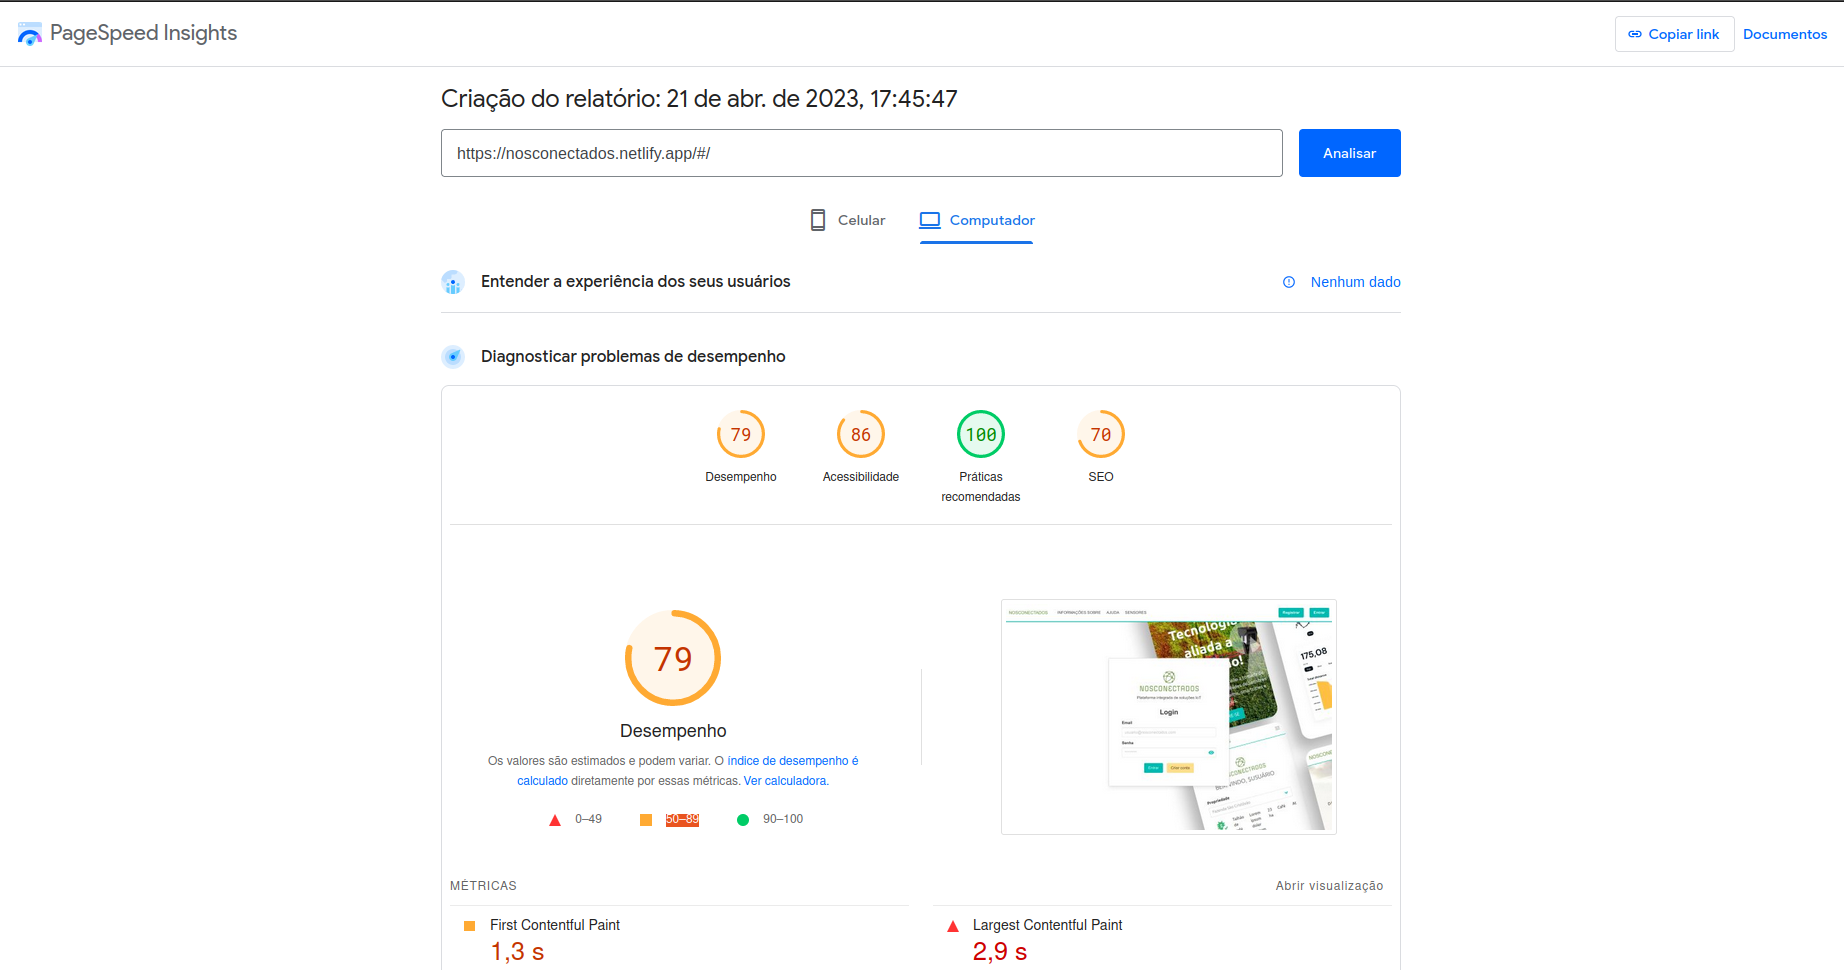
\includegraphics[scale=.25]{assets/desempenho-home.png}
  \caption{Teste de aceitação da página inicial}
  \label{teste-home}
\end{figure}

A rapidez com que uma página é carregada e exibida no navegador do usuário, conhecida como desempenho, é um dos aspectos avaliados no relatório de testes. Um bom desempenho é fundamental para evitar que os visitantes do site abandonem a página devido a tempos de carregamento longos. Para otimizar o desempenho, podem ser aplicadas várias técnicas, como otimização de imagens, uso de cache, minificação de arquivos CSS e JavaScript, entre outras. Além disso, o servidor de hospedagem também desempenha um papel importante na performance de uma página. Como estamos usando o serviço gratuito do Netlify, é possível que haja algumas limitações que impactem o desempenho, mas ainda assim, é possível ver que a página se mantém dentro dos padrões estabelecidos pelo PageSpeed.

Outro parâmetro avaliado é a acessibilidade, que se refere à capacidade de uma página ser facilmente utilizada e compreendida por todos os usuários, independentemente de suas habilidades ou deficiências. É importante garantir que a página seja acessível para pessoas com deficiência visual, auditiva, motora ou cognitiva. Isso pode envolver o uso de marcação semântica correta, fornecimento de alternativas textuais para imagens, uso adequado de cores, entre outras práticas.

Além disso, são avaliadas as técnicas recomendadas, que são práticas de desenvolvimento web consideradas melhores práticas pela comunidade de desenvolvedores. Essas práticas visam garantir que o site seja construído de forma eficiente, segura e de acordo com os padrões e diretrizes estabelecidos. Isso pode incluir o uso de HTML e CSS válidos, estruturação semântica do conteúdo, implementação de URLs amigáveis, entre outros aspectos.

Por fim, o SEO é outro parâmetro avaliado no relatório de testes. O SEO, ou Otimização para Mecanismos de Busca, é um conjunto de estratégias utilizadas para melhorar a visibilidade de um site nos resultados de busca orgânica. Isso pode envolver a otimização de elementos como palavras-chave, metatags, estrutura de URLs, título e descrição das páginas, além de outros fatores técnicos e de conteúdo. O objetivo é tornar o site mais relevante para os mecanismos de busca, o que pode resultar em uma melhor classificação nas páginas de resultados de busca e aumento do tráfego orgânico.

Na figura \ref{teste-ajuda} é possível ver o relatório de testes para a página de ajuda da plataforma.
\begin{figure}[htbp]
  \centering 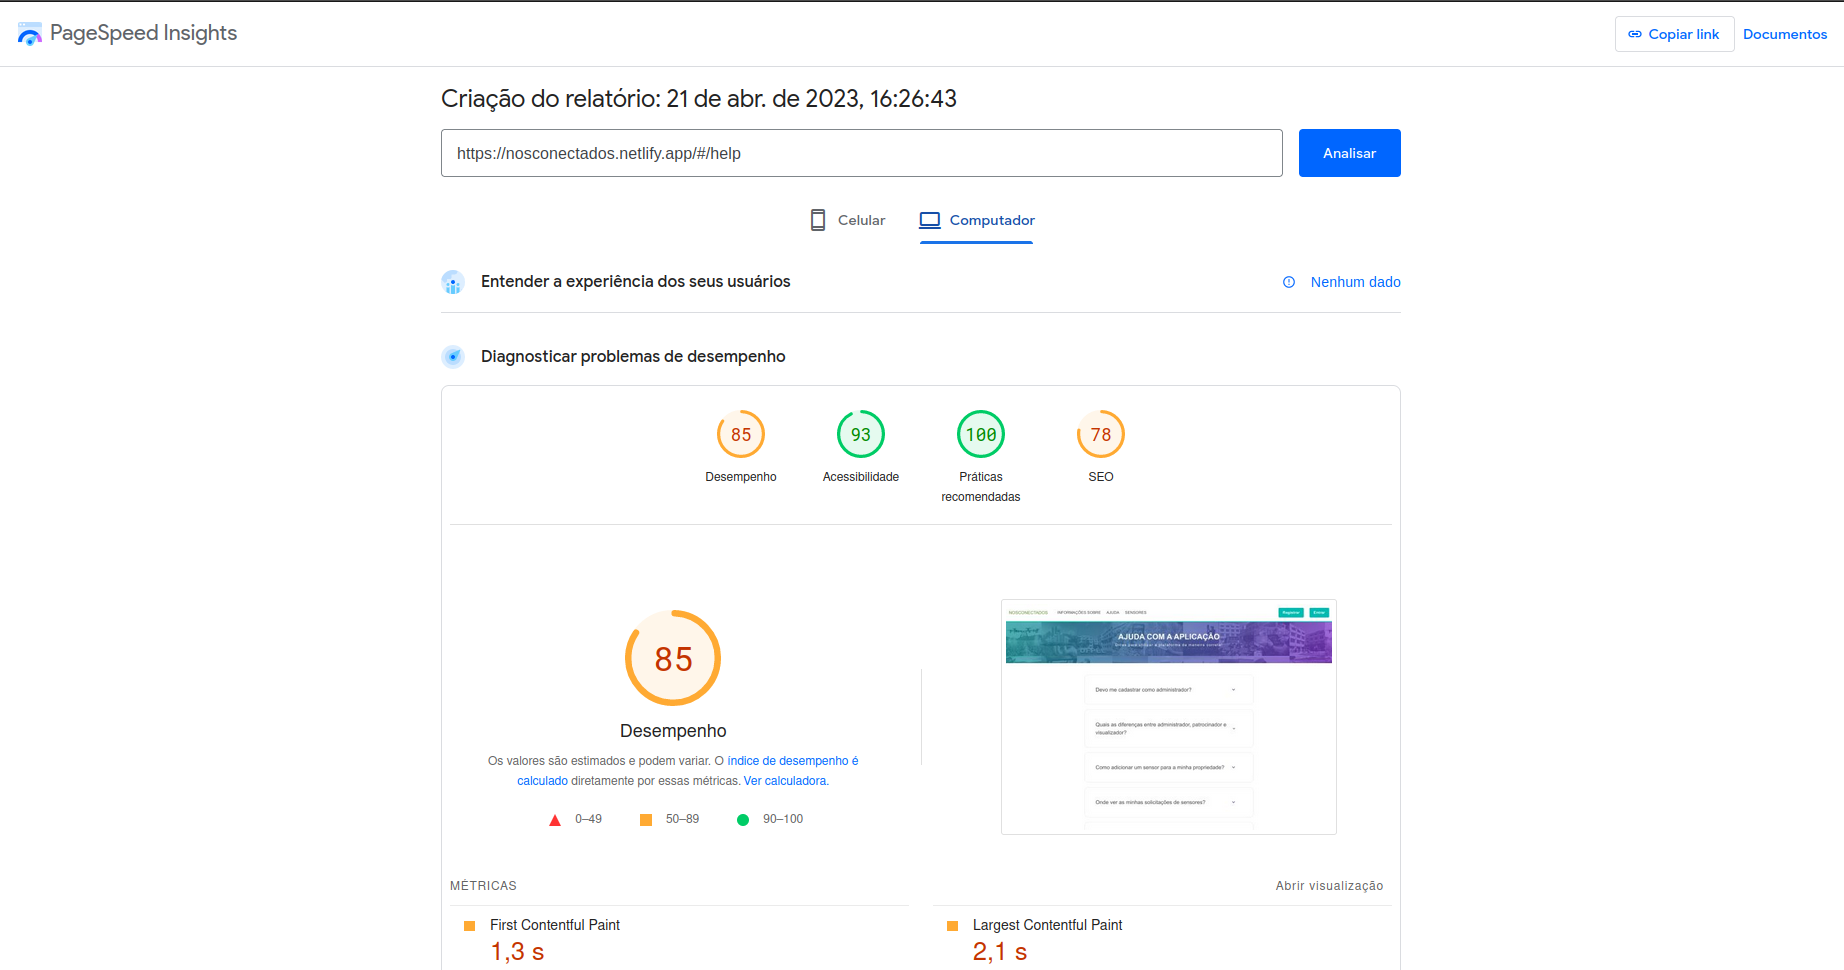
\includegraphics[scale=.25]{assets/desempenho-ajuda.png}
  \caption{Teste de aceitação da página de ajuda}
  \label{teste-ajuda}
\end{figure}

Ao comparar o relatório da página inicial com o atual, é evidente um significativo ganho de desempenho. Nota-se que a redução do número de imagens contribuiu para um melhor desempenho da página, com tempos de carregamento mais rápidos. Além disso, a presença de conteúdo textual e informativo relevante na página também colaborou para uma maior acessibilidade, tornando o site mais inclusivo para diversos tipos de usuários. É relevante ressaltar que a página obteve nota máxima em práticas recomendadas, o que indica a adesão a boas práticas de desenvolvimento.

Na figura \ref{teste-sobre} é possível ver o relatório de testes para a página de informações da plataforma.

\begin{figure}[htbp]
  \centering 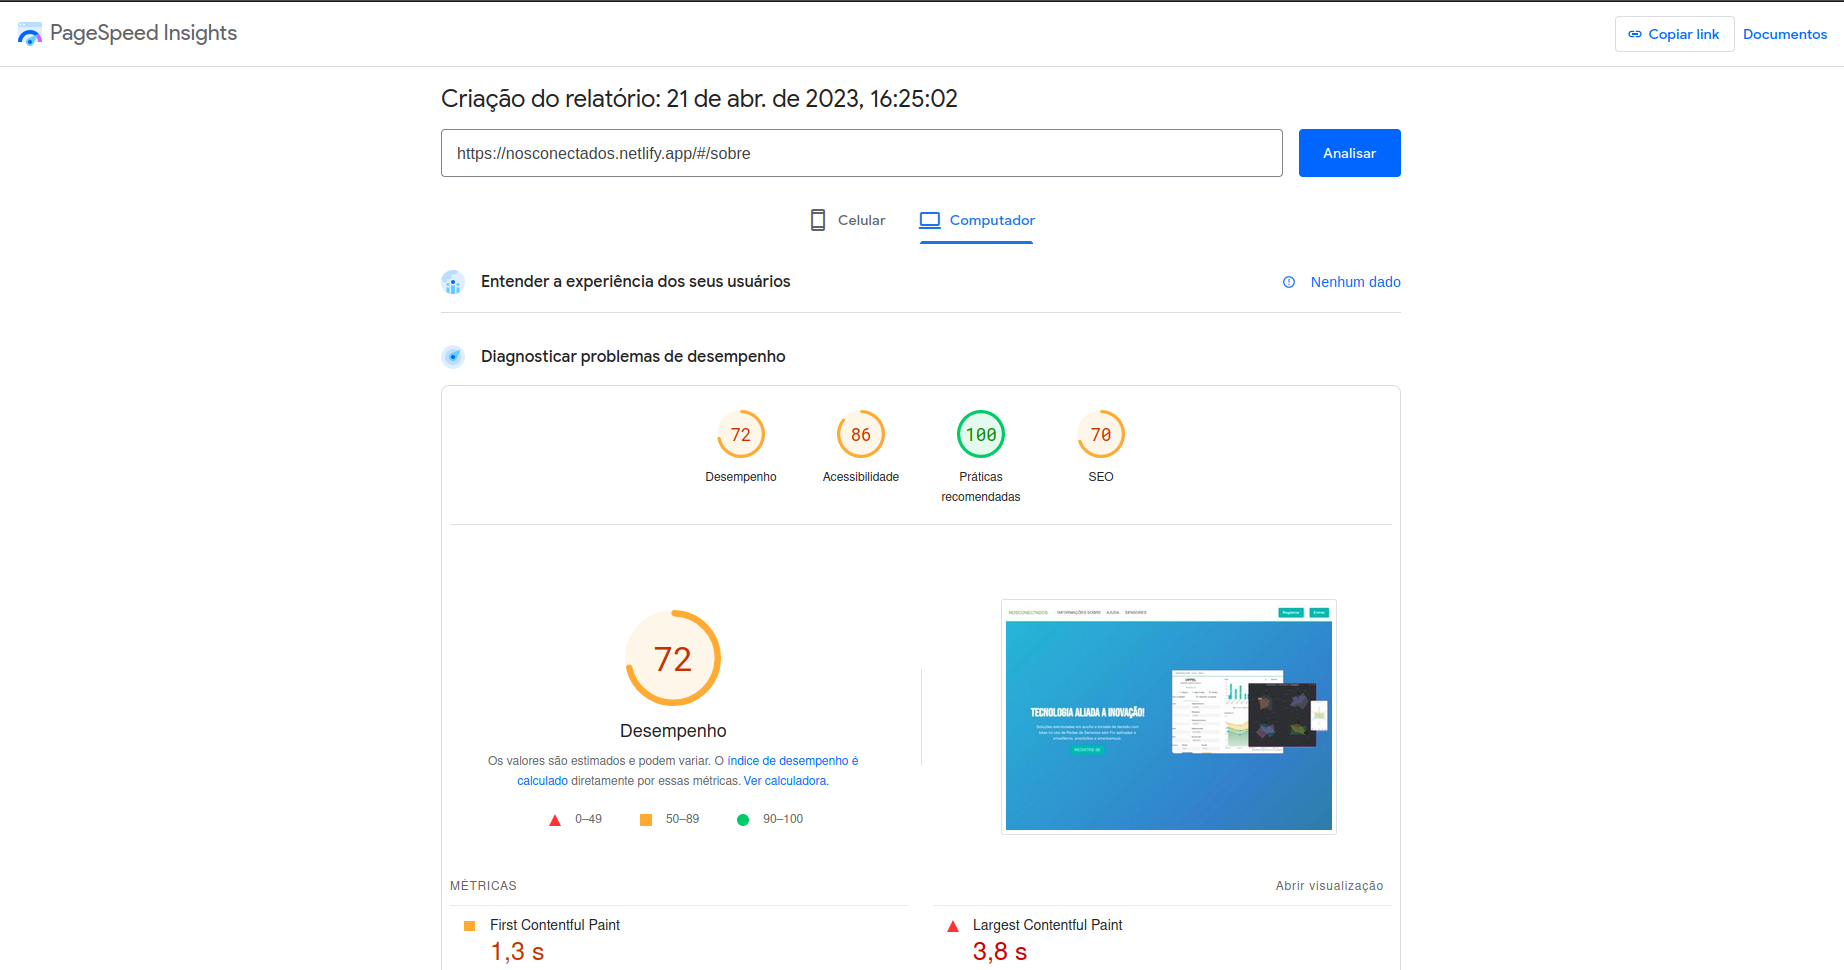
\includegraphics[scale=.25]{assets/desempenho-sobre.png}
  \caption{Teste de aceitação da página de informações}
  \label{teste-sobre}
\end{figure}

Ao comparar com relatórios anteriores, é possível observar uma diminuição do desempenho, o que pode ser atribuído ao alto número de imagens carregadas na página. É importante ressaltar que a otimização de imagens é um fator crucial para o desempenho de uma página, e o excesso de imagens pode impactar negativamente no tempo de carregamento. No entanto, é compreensível que o uso de imagens seja considerado essencial no contexto desta página específica. Apesar desse desafio, é notável que a página ainda mantém um alto nível de conformidade com as práticas recomendadas, obtendo nota máxima nesse quesito. 

Na figura \ref{teste-sobre} é possível ver o relatório de testes para a página de sensores públicos da plataforma.

\begin{figure}[htbp]
  \centering 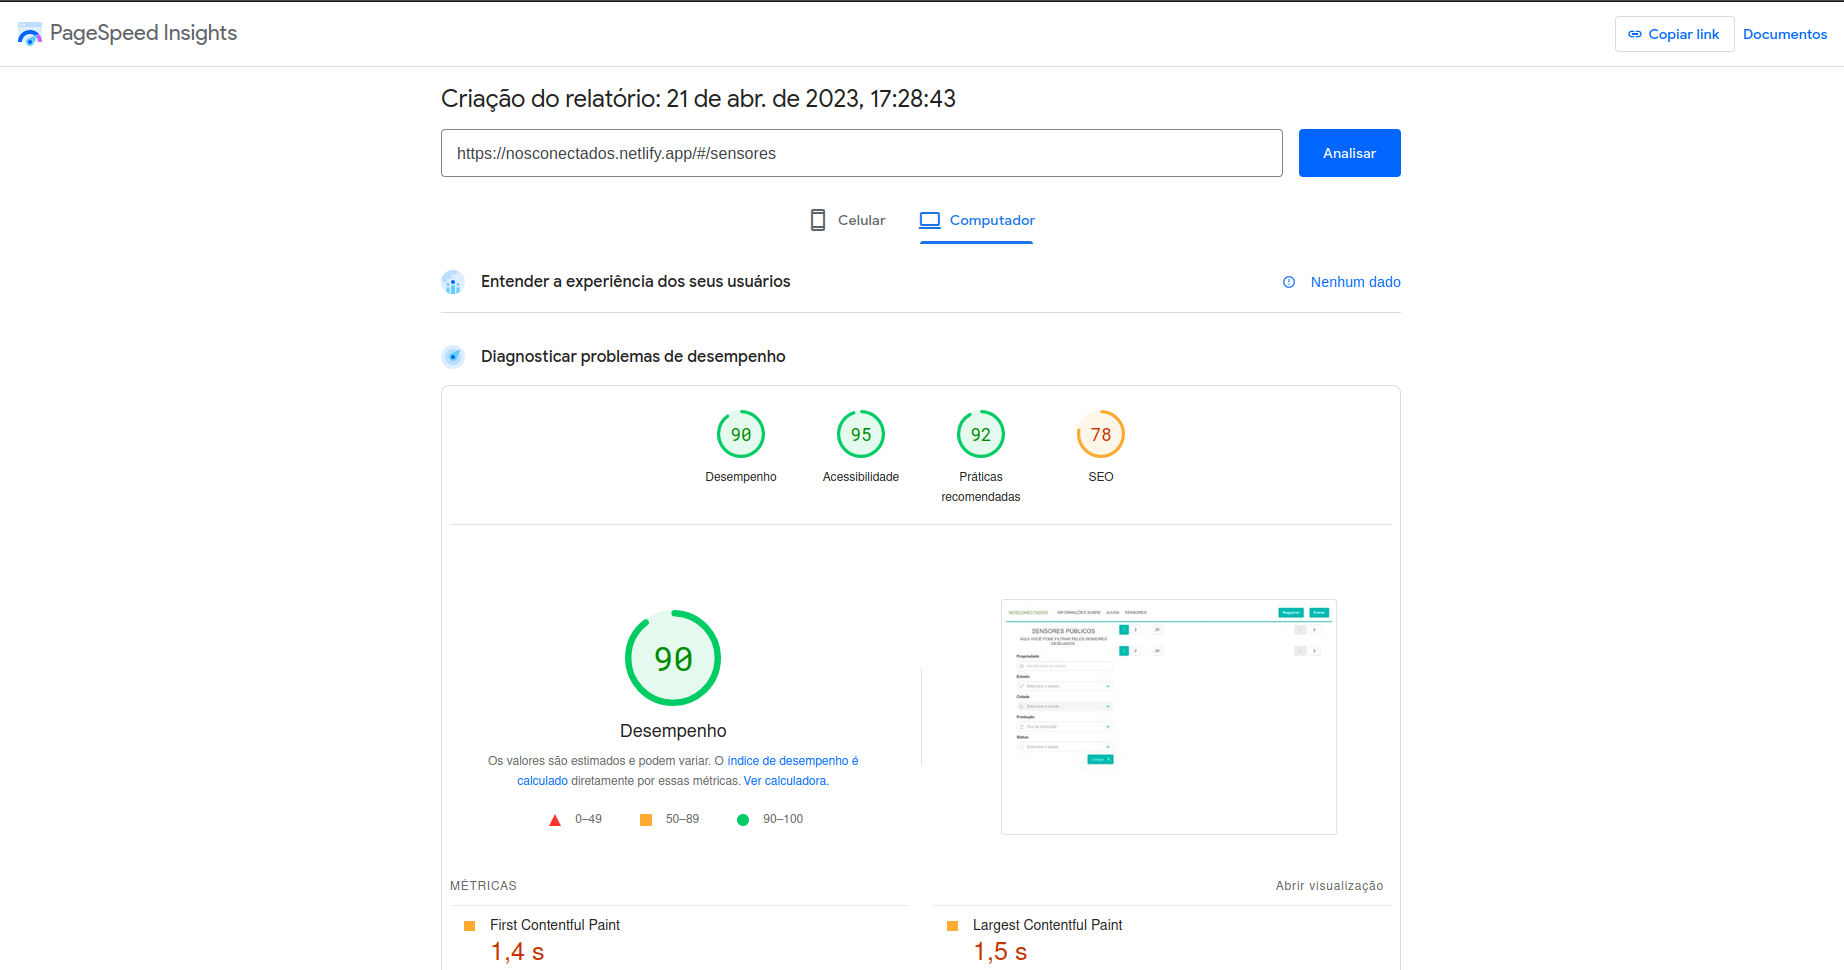
\includegraphics[scale=.25]{assets/desempenho-sensores.png}
  \caption{Teste de aceitação da página de sensores públicos}
  \label{teste-sensores}
\end{figure}
\newpage
Foi observado que o desempenho desta página em particular foi consideravelmente superior em comparação com outras páginas, devido à ausência de imagens. Essa página em questão apresenta apenas informações dos sensores, com uma filtragem no lado esquerdo e os dados dos sensores em formato de texto no lado direito. Essa abordagem de design mais minimalista, sem o uso de imagens, contribuiu significativamente para melhorar o desempenho da página. A ausência de elementos visuais complexos, como imagens, reduziu o tempo de carregamento da página, tornando-a mais rápida e eficiente para os usuários.

Na figura \ref{teste-registro}, é possível observar o teste da página de registro, em que a taxa de desempenho se mantém estável em relação às demais páginas. No entanto, a acessibilidade da página diminuiu consideravelmente. Essa questão será abordada na seção \ref{sec:manutencao}, em que serão propostas possíveis melhorias, como a adoção de nomes mais específicos para as imagens, a fim de auxiliar o usuário final, e a aplicação de boas práticas para garantir uma melhor acessibilidade.
\begin{figure}[htbp]
  \centering 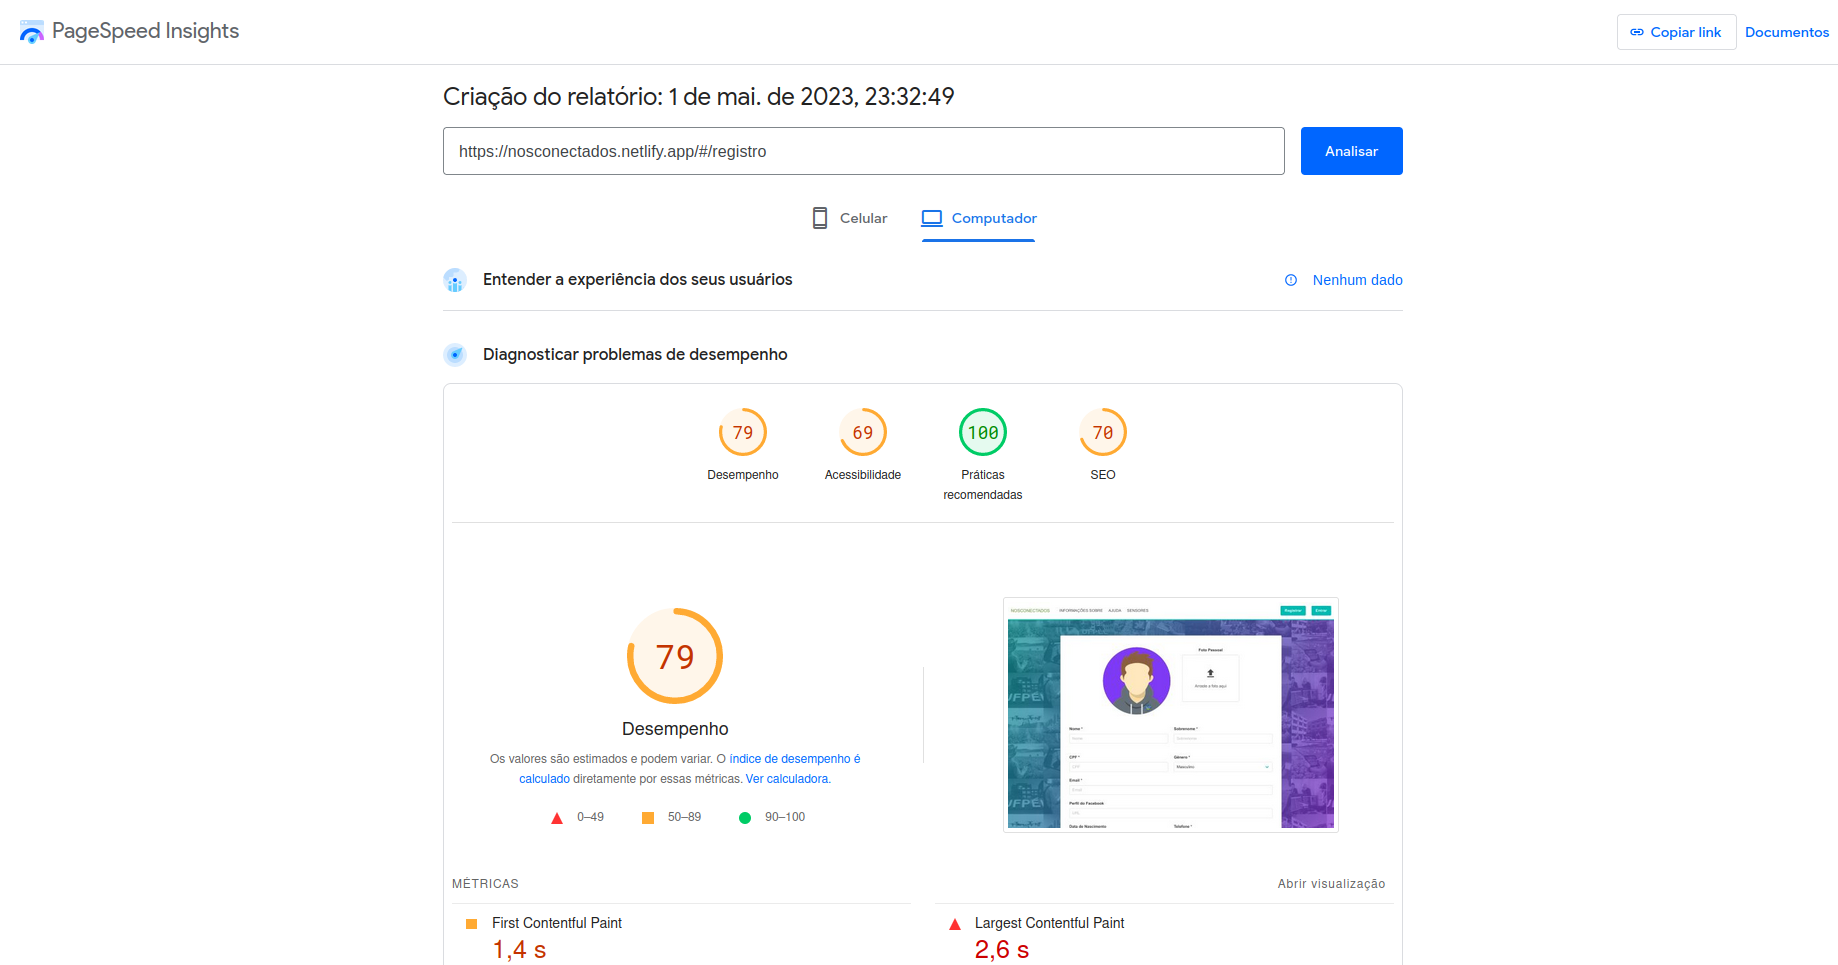
\includegraphics[scale=.25]{assets/testeregistro.png}
  \caption{Teste de aceitação da página de registro}
  \label{teste-registro}
\end{figure}
\newpage
Dessa forma, em ambiente de produção, é possível realizar os testes de aceitação em todas as páginas que não requerem autenticação do usuário. Já as páginas que estão protegidas pelo middlewareAuth só podem ser testadas localmente. Entretanto, foi possível identificar um padrão bem específico entre as páginas, pois todos os requisitos foram atendidos com sucesso, conforme indicado pelos relatórios do PageSpeed. Esses relatórios fornecem sugestões de possíveis melhorias que podem ser feitas nas páginas para aprimorar seus aspectos.


\section{Documentação}
\label{sec:documentacao}
A documentação é uma etapa importante do processo de desenvolvimento de software, uma vez que permite a compreensão e utilização adequada da plataforma pelos usuários finais e pelos desenvolvedores envolvidos no projeto. Nesta seção, serão apresentadas as etapas de documentação da nossa plataforma.

A documentação técnica é destinada aos desenvolvedores e visa auxiliar na manutenção e evolução do projeto. Para esta finalidade, foram utilizadas bibliotecas específicas de documentação em cada uma das tecnologias utilizadas. Para o front-end, foi utilizada a biblioteca Vue Styleguidist \cite{VueStyleguidist:2023}, que permite a geração de documentação do Vue.js \cite{vue:2014} com Buefy \cite{buefy:2022}, Bulma \cite{bulma:2022} e Bootstrap \cite{bootstrap:2023} de forma automática. Já no back-end, a biblioteca PHPDocumentor \cite{PHPDocumentor:2023} foi utilizada para documentar o código PHP \cite{PHP:2022} com PDO \cite{PDO:2022} e Slim Framework \cite{slim:2023}. Além disso, a documentação técnica também incluem os diagramas criados na etapa de modelagem, que descrevem a estrutura do sistema.

Para a documentação da API, foram disponibilizadas as coleções do Postman \cite{Postman:2023}, que possuem todas as rotas, parâmetros e exemplos de requisições e respostas da API. Isso facilita a compreensão e utilização da plataforma por parte dos desenvolvedores interessados em integrar seus sistemas com a nossa API. Além disso, a documentação também inclui uma descrição detalhada de cada rota da API, juntamente com exemplos de entrada e saída de dados. Dessa forma, é possível garantir uma integração fácil e eficiente da plataforma com outros sistemas, o que aumenta a sua utilidade e relevância para os usuários finais.

É fundamental destacar que toda a documentação pública da plataforma, excluindo o código e seus comentários, bem como as variáveis de ambiente e as senhas para as plataformas de deploy, está disponível em um repositório no Github acessível pelo link \href{https://github.com/HuberM1998/nosconectados}{https://github.com/HuberM1998/nosconectados}. Qualquer pessoa pode acessar este repositório de documentação, que contém informações importantes tanto para os desenvolvedores quanto para aqueles que desejam compreender a estrutura da plataforma e suas funcionalidades. Além disso, as coleções do Postman para o ambiente de desenvolvimento também estão incluídas no repositório.

A documentação para o usuário final tem como objetivo apresentar a plataforma e suas funcionalidades de forma clara e objetiva. Para isso foi criado uma página denominada "Ajuda"\space que está disponível na barra de navegação da plataforma contendo uma seção de perguntas frequentes que aborda as principais dúvidas dos usuários em relação ao uso da plataforma e pode ser visualizada na seção \ref{sec:paginaajuda} na figura \ref{ajuda}.

Por fim, a documentação de código tem como objetivo facilitar a compreensão e manutenção do código-fonte do projeto. Para isso, foram utilizados comentários no código seguindo as convenções das bibliotecas de documentação utilizadas. Além disso, foram criados arquivos README.md nos repositórios do projeto, que contém informações sobre a instalação e utilização da plataforma, bem como sobre as tecnologias utilizadas e as bibliotecas de terceiros. Com a documentação técnica, documentação para o usuário final e documentação de código, é possível garantir uma melhor compreensão e utilização da plataforma.
\section{Manutenção}
\label{sec:manutencao}
A seção de manutenção é uma etapa crucial no ciclo de vida de qualquer software. Mesmo após o lançamento da plataforma, é importante que a manutenção seja realizada periodicamente para garantir que o sistema continue funcionando corretamente e sem interrupções. 

Na etapa de Desenvolvimento descrita na seção \ref{sec:desenvolvimento}, foram utilizadas diversas tecnologias, incluindo Vue.js \cite{vue:2014}, Buefy \cite{buefy:2022}, Bulma \cite{bulma:2022}, PHP \cite{PHP:2022}, PDO \cite{PDO:2022}, Slim Framework \cite{slim:2023} e MySQL \cite{mysql:2022}. É importante que, durante a manutenção, as versões dessas tecnologias sejam atualizadas para evitar vulnerabilidades de segurança e incompatibilidades. Da mesma forma com a seção \ref{sec:testes} e \ref{sec:documentacao}.

Além disso, é importante que a manutenção inclua a correção de quaisquer bugs ou falhas que possam surgir no sistema, bem como a atualização de recursos e funcionalidades. Isso pode incluir a adição de novos recursos, aprimoramentos de segurança e correções de erros de usabilidade.

Para possíveis melhorias futuras, destacamos a utilização de arquivos para a importação de dados na plataforma. Além disso, para sensores mais antigos, é possível remover a autenticação JWT de 256 bits e realizar a autenticação diretamente no servidor por meio do CORS, permitindo apenas que os IPs dos sensores autorizados enviem dados. Essa melhoria é específica para permitir a inclusão de toda a base de dados da Agência de Desenvolvimento da Bacia da Lagoa Mirim na plataforma, considerando que alguns sensores possuem capacidade de memória limitada e não suportam o armazenamento de tokens. Além disso, existem sensores que coletam dados de forma manual e precisam ser inseridos na plataforma manualmente.

A partir dos testes de aceitação realizados na plataforma em produção, conforme descrito na seção \ref{sec:testes}, foi possível identificar lacunas a serem preenchidas nessa etapa. Com base nos relatórios gerados pelo PageSpeed Insights, é possível aprimorar aspectos relevantes em termos de acessibilidade e desempenho da plataforma. Com isso, é possível melhorar a plataforma durante a manutenção, tornando-a mais rápida e acessível, o que consequentemente melhora a experiência do usuário.

Ademais, dentre as possíveis melhorias, salienta-se a implementação da funcionalidade de recuperação de senha, bem como a incorporação de outros métodos de autenticação, como o uso do protocolo OAuth para permitir o login de usuários a partir de plataformas conhecidas como Google, Facebook e Github.
\chapter{Visão das telas}
Com base nos testes realizados na plataforma em produção, podemos concluir que ela atingiu com êxito o objetivo proposto no escopo do projeto. Além disso, os resultados obtidos demonstram que a plataforma apresenta ótima performance e usabilidade. A interface gráfica é intuitiva e de fácil navegação, o que contribui para uma experiência satisfatória para os usuários.

A apresentação da plataforma foi feita através de capturas de tela, que mostraram a estrutura organizada dos menus e botões, bem como a visualização dos dados coletados pelos sensores. A página de painel do administrador, por exemplo, apresentou uma visão clara das informações e atribuições dos sensores, permitindo ao administrador gerenciá-los de forma eficiente.

Outra parte importante deste trabalho foi o desenvolvimento da API, que fornece as funcionalidades necessárias para a comunicação entre a plataforma e os dispositivos de sensoriamento. A API foi desenvolvida utilizando a arquitetura RESTful e disponibiliza endpoints para o acesso aos dados dos sensores, cadastro e remoção de sensores, além de outras funcionalidades.

No que diz respeito à estrutura da API, foram definidas rotas para as principais funcionalidades da plataforma, como listagem de sensores, cadastro de novos sensores e visualização dos dados coletados pelos sensores. Além disso, foram implementados mecanismos de autenticação e autorização para garantir a segurança e a privacidade dos dados coletados pelos sensores.

Há muito mais a ser explorado nesta plataforma, como a implementação de análises de dados e a possibilidade de integração com outras ferramentas, o que pode torná-la ainda mais poderosa e versátil.\space A disponibilidade online da plataforma e da API no endereço \href{https://nosconectados.netlify.app/}{https://nosconectados.netlify.app/} e \href{https://nosconectados.herokuapp.com/public/}{https://nosconectados.herokuapp.com/public/}, respectivamente, permite que os usuários acessem e utilizem a plataforma de forma prática e acessível em qualquer lugar e momento.

Dessa forma, a seção atual apresenta a plataforma desenvolvida, demonstrando como foram implementadas as principais funcionalidades e como a comunicação entre a plataforma e os sensores foi realizada de forma eficiente e segura. Além disso, ressalta-se o potencial desta plataforma para o monitoramento de dados em redes de sensores sem fio e as possibilidades de melhorias e expansões futuras.
\section{Apresentação da plataforma}
A seção de apresentação da plataforma é um momento importante para destacar as funcionalidades e a aparência da interface. Nesta seção, é fornecida uma visão geral da plataforma, para que o leitor possa entender como ela funciona e o que ela oferece.

Ao apresentar as telas da plataforma, é destacado os recursos mais importantes de cada página. Por exemplo, a página de login deve permitir que os usuários façam login com segurança, enquanto a página de painel do administrador deve exibir informações relevantes sobre os sensores e usuários cadastrados na plataforma.

Para apresentar as telas, é utilizado imagens de capturas de tela da própria plataforma, mostrando uma versão disponível para desktop e uma para mobile para que o leitor possa ter uma ideia clara do que a plataforma oferece e a sua responsividade. Além disso, descrevemos as funcionalidades de cada página e como elas se relacionam com outras partes da plataforma.

\subsection{Página inicial}
A página de início da plataforma é essencialmente informativa e funcional, com o objetivo de fornecer uma breve introdução aos usuários sobre o que a plataforma faz. A imagem de fundo, que é composta por vários gráficos conhecidos como dashboards, oferece aos usuários uma visão rápida das informações que podem ser acessadas por meio da plataforma.

No centro, destaca-se um card que contém um formulário de login. Esse formulário oferece aos usuários a possibilidade de fazer login ou criar uma conta. Essa abordagem permite que os usuários acessem rapidamente as funcionalidades da plataforma sem perder tempo em se cadastrar, caso já tenham uma conta na plataforma.

Se o login for bem-sucedido, o usuário será direcionado para a página de dashboard, onde poderá ver e analisar os dados coletados pela plataforma. Por outro lado, se o usuário não conseguir fazer login, ele permanecerá na mesma página inicial, permitindo que ele tente novamente ou crie uma nova conta.

Essa abordagem garante que a plataforma seja acessível e funcional para usuários de todos os níveis de habilidade e conhecimento. Além disso, oferece uma experiência simplificada para o usuário, com acesso fácil às informações da plataforma, o que pode aumentar a sua utilização. Na figura \ref{home} é possível ver como é a página inicial da plataforma.
\begin{figure}[htbp]
  \centering 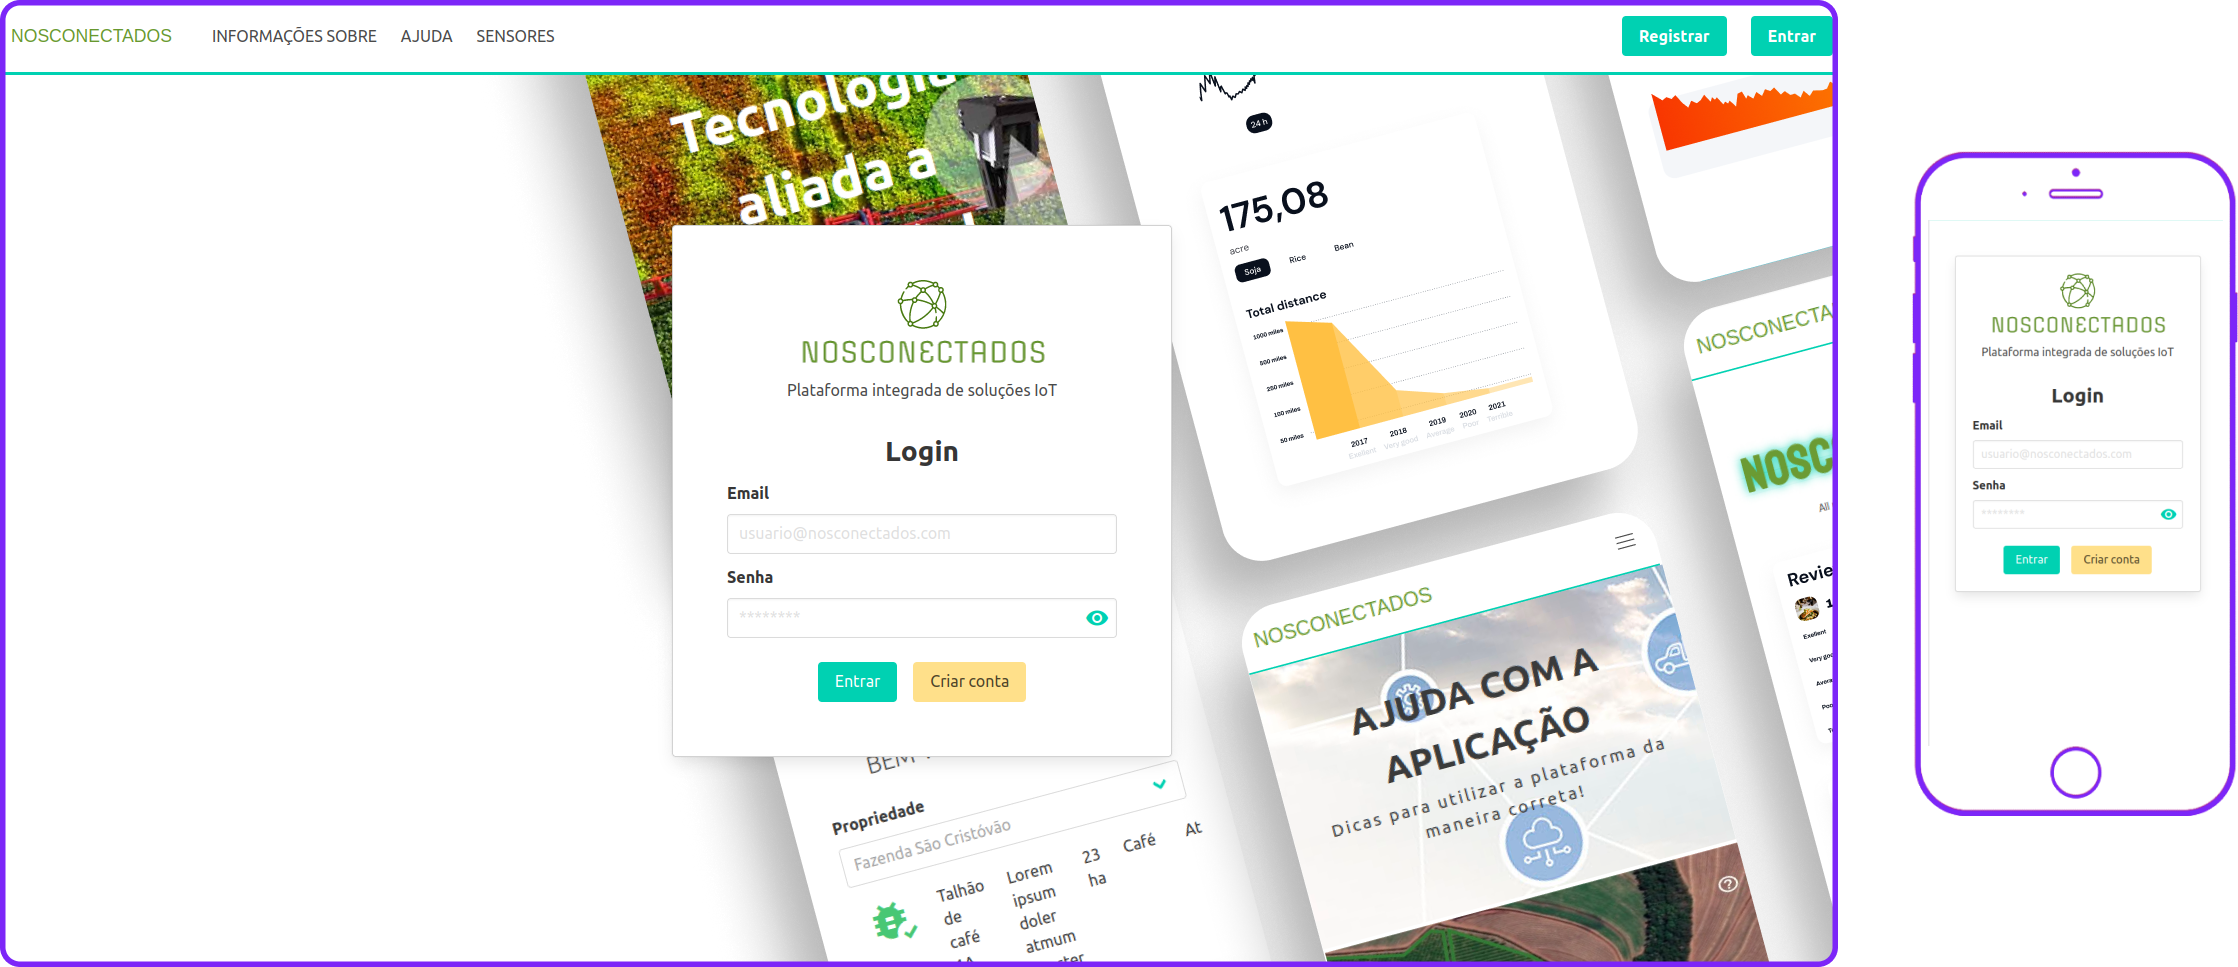
\includegraphics[scale=.2]{assets/home.png}
  \caption{Página inicial}
  \label{home}
\end{figure}

\subsection{Dashboard}
A página de dashboard é uma das páginas mais importantes da plataforma, pois é a primeira página que o usuário visualiza após logar na plataforma. Ela tem como objetivo apresentar de forma clara e concisa as informações dos sensores cadastrados pelo usuário. Na parte esquerda da página, o usuário pode visualizar uma lista com todos os seus sensores, incluindo informações como o status, a propriedade, a descrição, a área e a produção. Essas informações são importantes para que o usuário possa monitorar de forma eficiente seus sensores e identificar possíveis problemas.

Além disso, na parte esquerda da página, é possível alternar as informações que são mostradas, através de quatro botões: resumo, área, produção e localização. Isso permite que o usuário possa visualizar as informações de acordo com sua necessidade, facilitando a visualização e a análise dos dados.

Na parte direita da página, o usuário pode visualizar o mapa com a localização dos seus sensores. Quando um sensor é selecionado, ele é destacado no mapa e é possível ver suas informações de localização. Isso permite que o usuário tenha uma visão geral da distribuição dos seus sensores, o que pode ser útil para planejar futuras instalações ou para identificar possíveis problemas de cobertura.

Em geral, a página de dashboard é uma ferramenta fundamental para que o usuário possa monitorar e gerenciar seus sensores de forma eficiente e prática. Com ela, é possível visualizar de forma clara e concisa as informações dos sensores, o que pode ajudar o usuário a identificar possíveis problemas ou oportunidades de melhoria na sua rede de sensores. Na figura \ref{dashboard} é possível ver como é a página de dashboard. Na figura \ref{dashboardnull} é possível ver como é a página de dashboard quando o usuário não tem nenhum sensor.
\begin{figure}[htbp]
  \centering 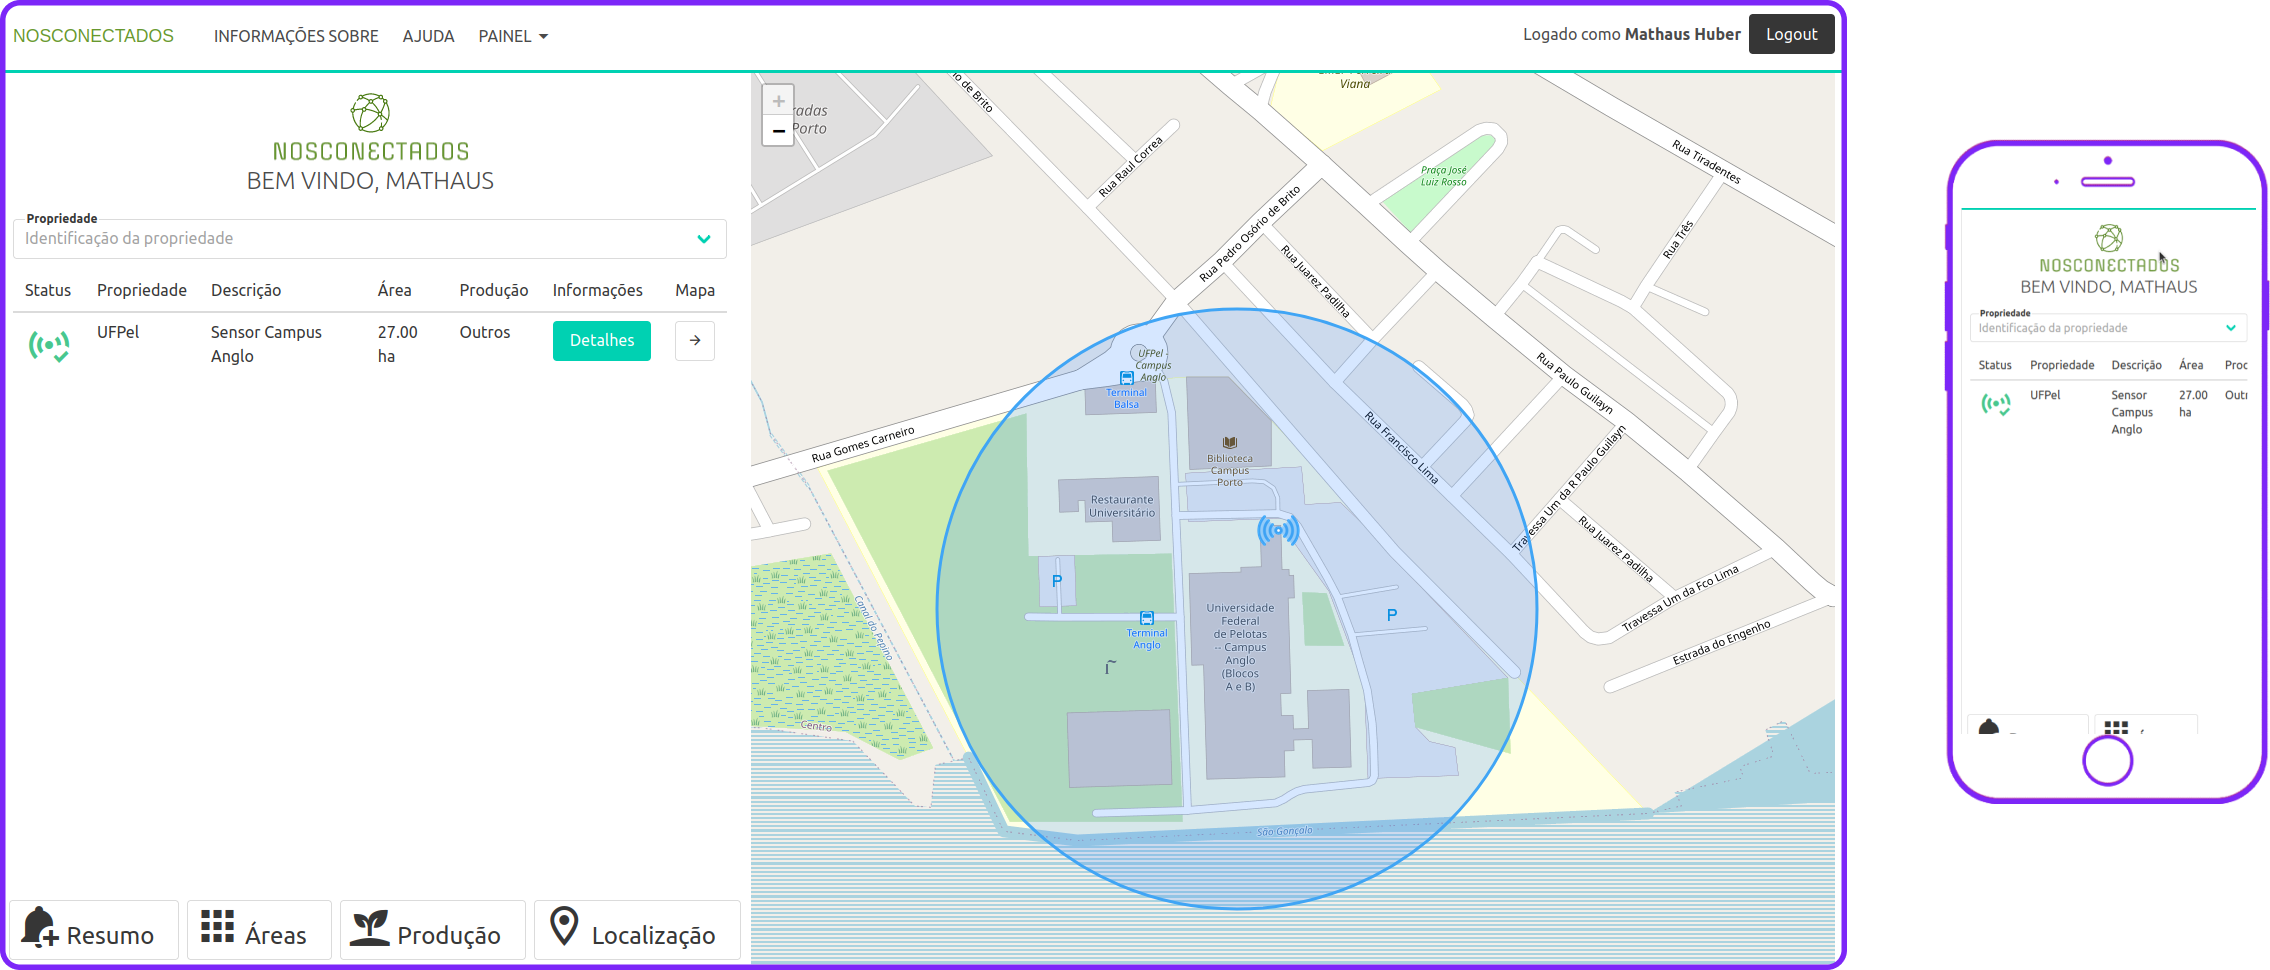
\includegraphics[scale=.2]{assets/dashboard.png}
  \caption{Página de dashboard}
  \label{dashboard}
\end{figure}

\begin{figure}[htbp]
  \centering 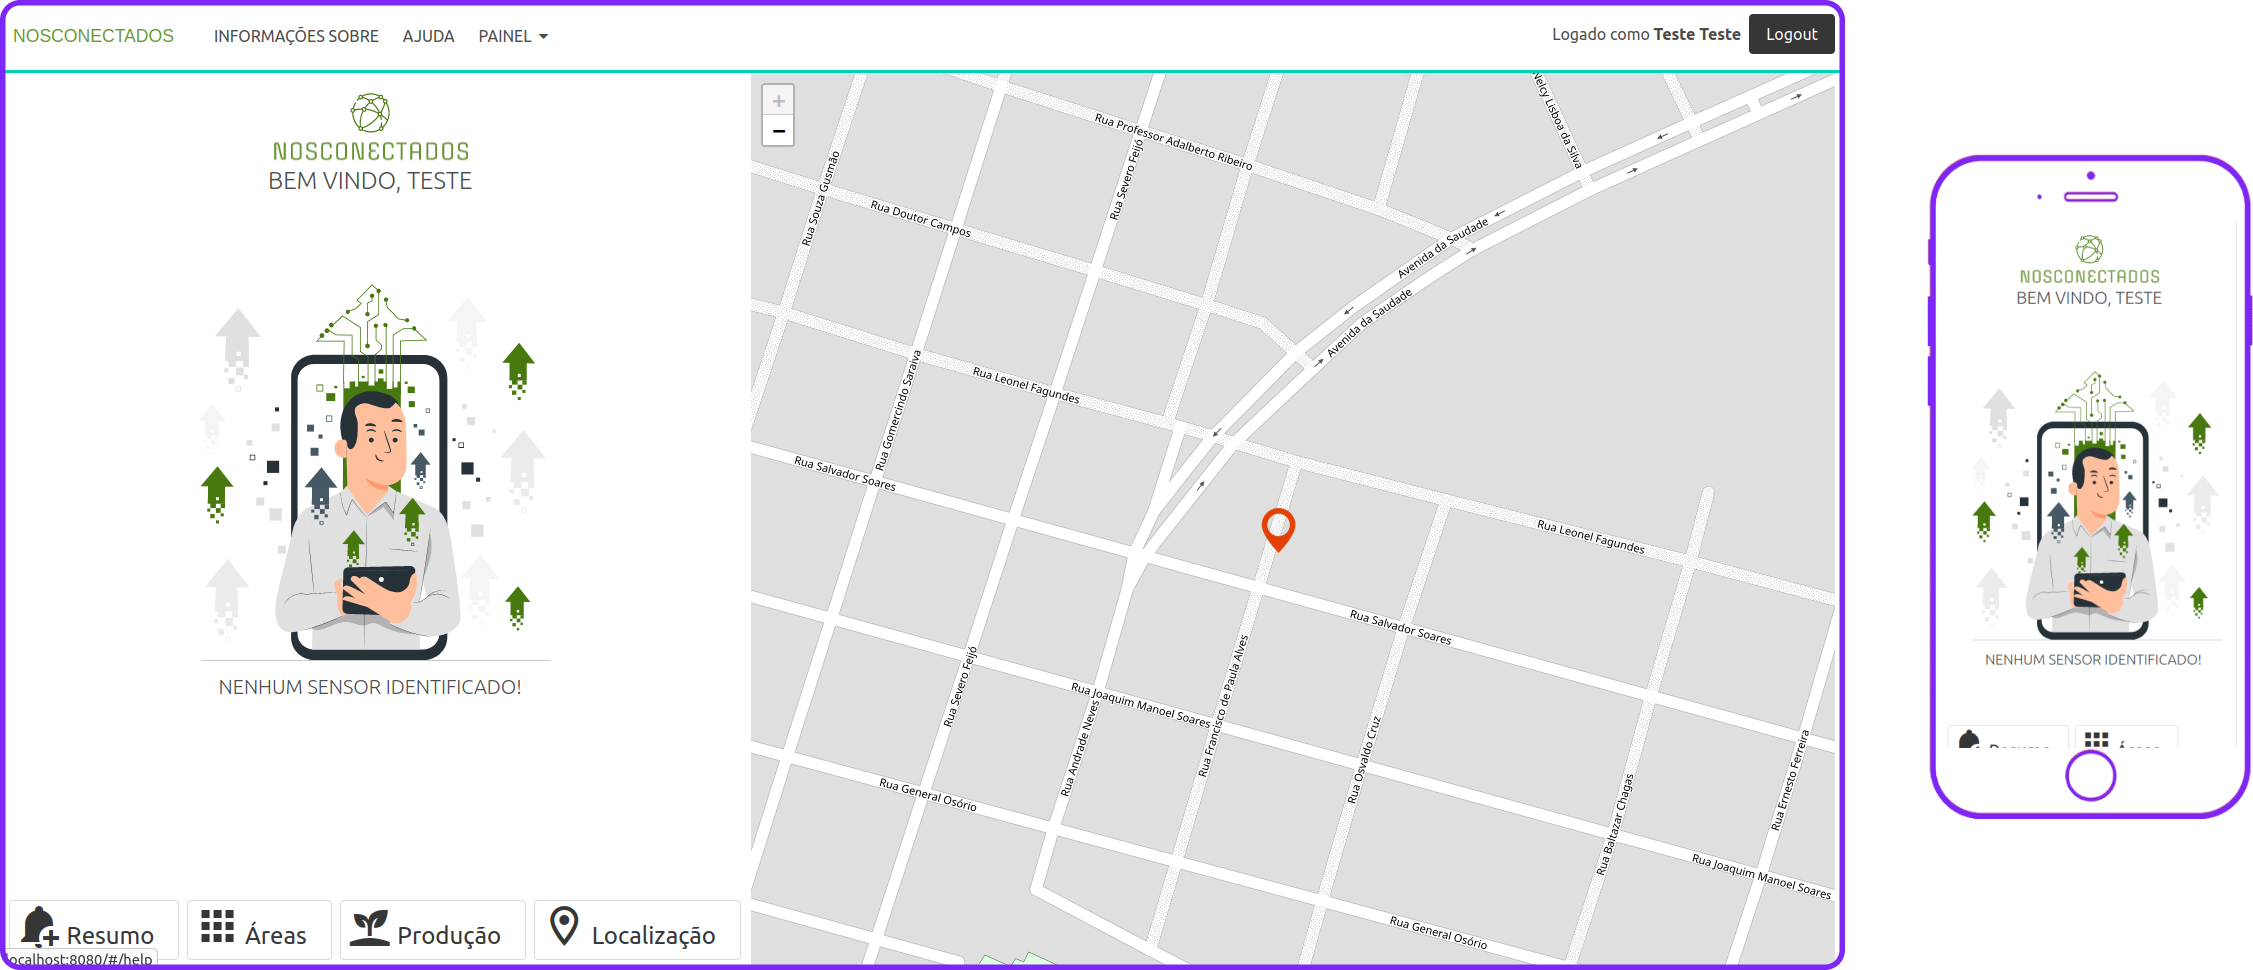
\includegraphics[scale=.2]{assets/dashboardnull.png}
  \caption{Página de dashboard quando não há nenhum sensor}
  \label{dashboardnull}
\end{figure}
\newpage
\subsection{Cadastro}
A página de registro é uma seção essencial para que os usuários possam acessar as funcionalidades da plataforma. Nessa página, o usuário deve inserir suas informações pessoais, essenciais e opcionais, para criar uma conta no sistema.

Entre as informações pessoais, estão o nome, sobrenome, CPF, gênero, e-mail, data de nascimento, CEP, telefone, bairro, rua, número, estado e município. Esses dados são necessários para que o usuário possa se identificar e criar uma conta na plataforma. É importante ressaltar que o CPF é um dado essencial, pois é ele que garante a autenticidade do usuário e ajuda a evitar fraudes na plataforma.

Além dos dados pessoais, a página de cadastro de também oferece a opção de inserir informações opcionais, como foto, complemento e perfil do Facebook. Essas informações podem ser úteis para personalizar a experiência do usuário na plataforma e facilitar a interação com outros usuários, se for o caso.

Por fim, a página de cadastro de usuários exige que o usuário insira uma senha segura e confirme a mesma. Isso garante a segurança das informações pessoais do usuário e evita o acesso não autorizado à sua conta. Em resumo, a página de cadastro de usuários é uma parte essencial no sistema para permitir o acesso do usuário às funcionalidades da plataforma. Com a coleta de informações pessoais e opcionais, a plataforma pode oferecer uma experiência personalizada e segura para o usuário. Na figura \ref{cadastro} é possível ver como é a página de cadastro.
\begin{figure}[htbp]
  \centering 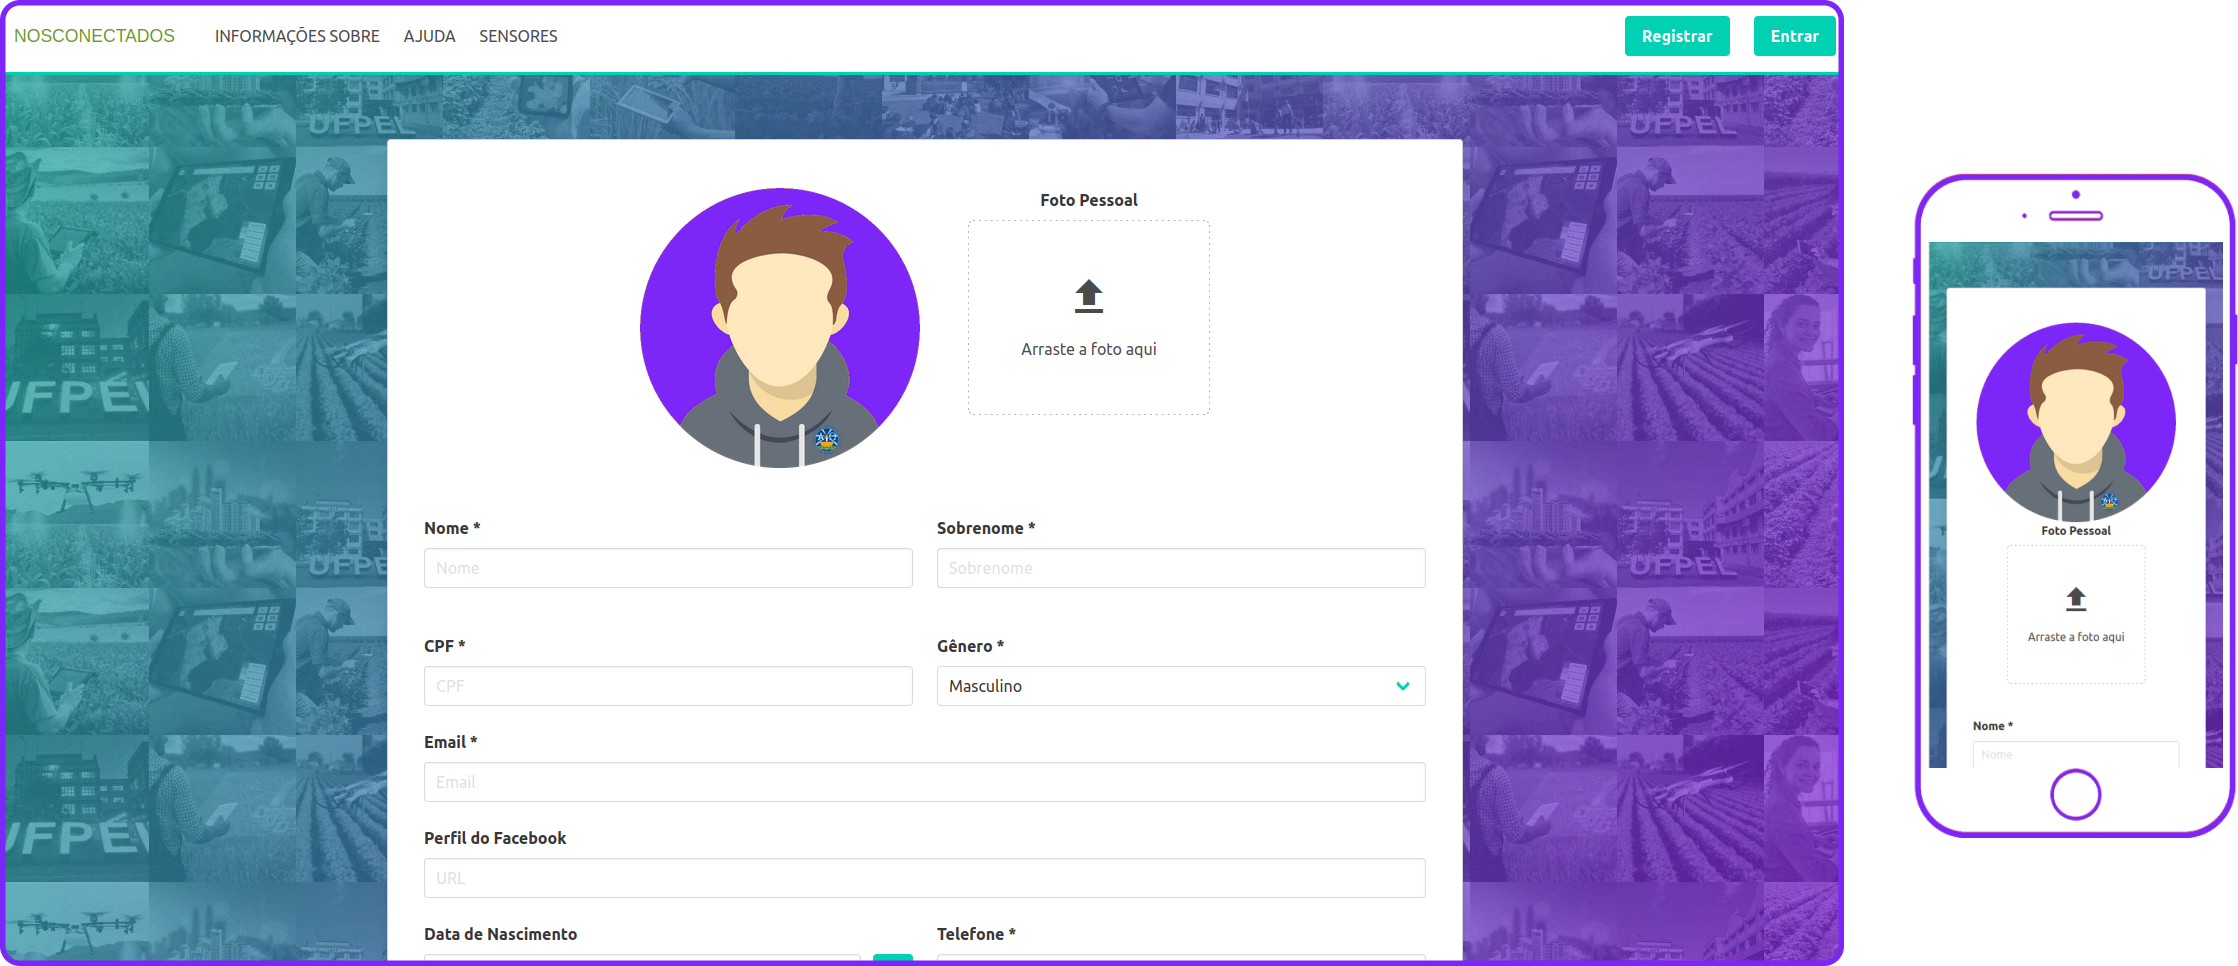
\includegraphics[scale=.2]{assets/cadastro.png}
  \caption{Página de registro de usuários}
  \label{cadastro}
\end{figure}
\newpage
\subsection{Sensores públicos}
A página de sensores públicos é uma seção que permite aos usuários verem informações importantes sobre os sensores instalados em diferentes locais. Na página, os usuários podem filtrar os sensores de acordo com sua propriedade, estado, cidade, tipo de produção e status.

A opção de filtrar por nome de propriedade é particularmente útil para usuários que desejam ver apenas os sensores instalados em uma determinada propriedade. Já o filtro por estado e cidade é útil para os usuários que desejam ver sensores específicos em uma região geográfica. O filtro por tipo de produção é relevante para usuários que desejam monitorar sensores relacionados a um determinado tipo de produção agrícola, por exemplo. Por fim, o filtro de status ajuda os usuários a visualizar apenas sensores ativos, inativos ou pendentes.

À direita da página de sensores públicos, os usuários podem ver os sensores que correspondem aos critérios de filtro selecionados. Cada sensor é apresentado em um card, que contém informações como nome do sensor, propriedade onde está instalado, tipo de produção, localização geográfica e status. O botão no meio do card permite que os usuários acessem informações mais detalhadas sobre o sensor.

Em resumo, a página de sensores públicos é uma ferramenta valiosa para usuários no sistema, pois permite que eles visualizem informações importantes sobre sensores instalados em diferentes locais. A opção de filtragem por diferentes critérios torna mais fácil encontrar os sensores desejados, enquanto o botão para acessar informações detalhadas do sensor ajuda a garantir que os usuários obtenham informações mais aprofundadas sobre o sensor específico que estão interessados.  Na figura \ref{publicos} é possível ver como é a página de sensores públicos. Na figura \ref{publicosnull} é possível ver como é a página de sensores públicos quando não há nenhum sensor.
\begin{figure}[htbp]
  \centering 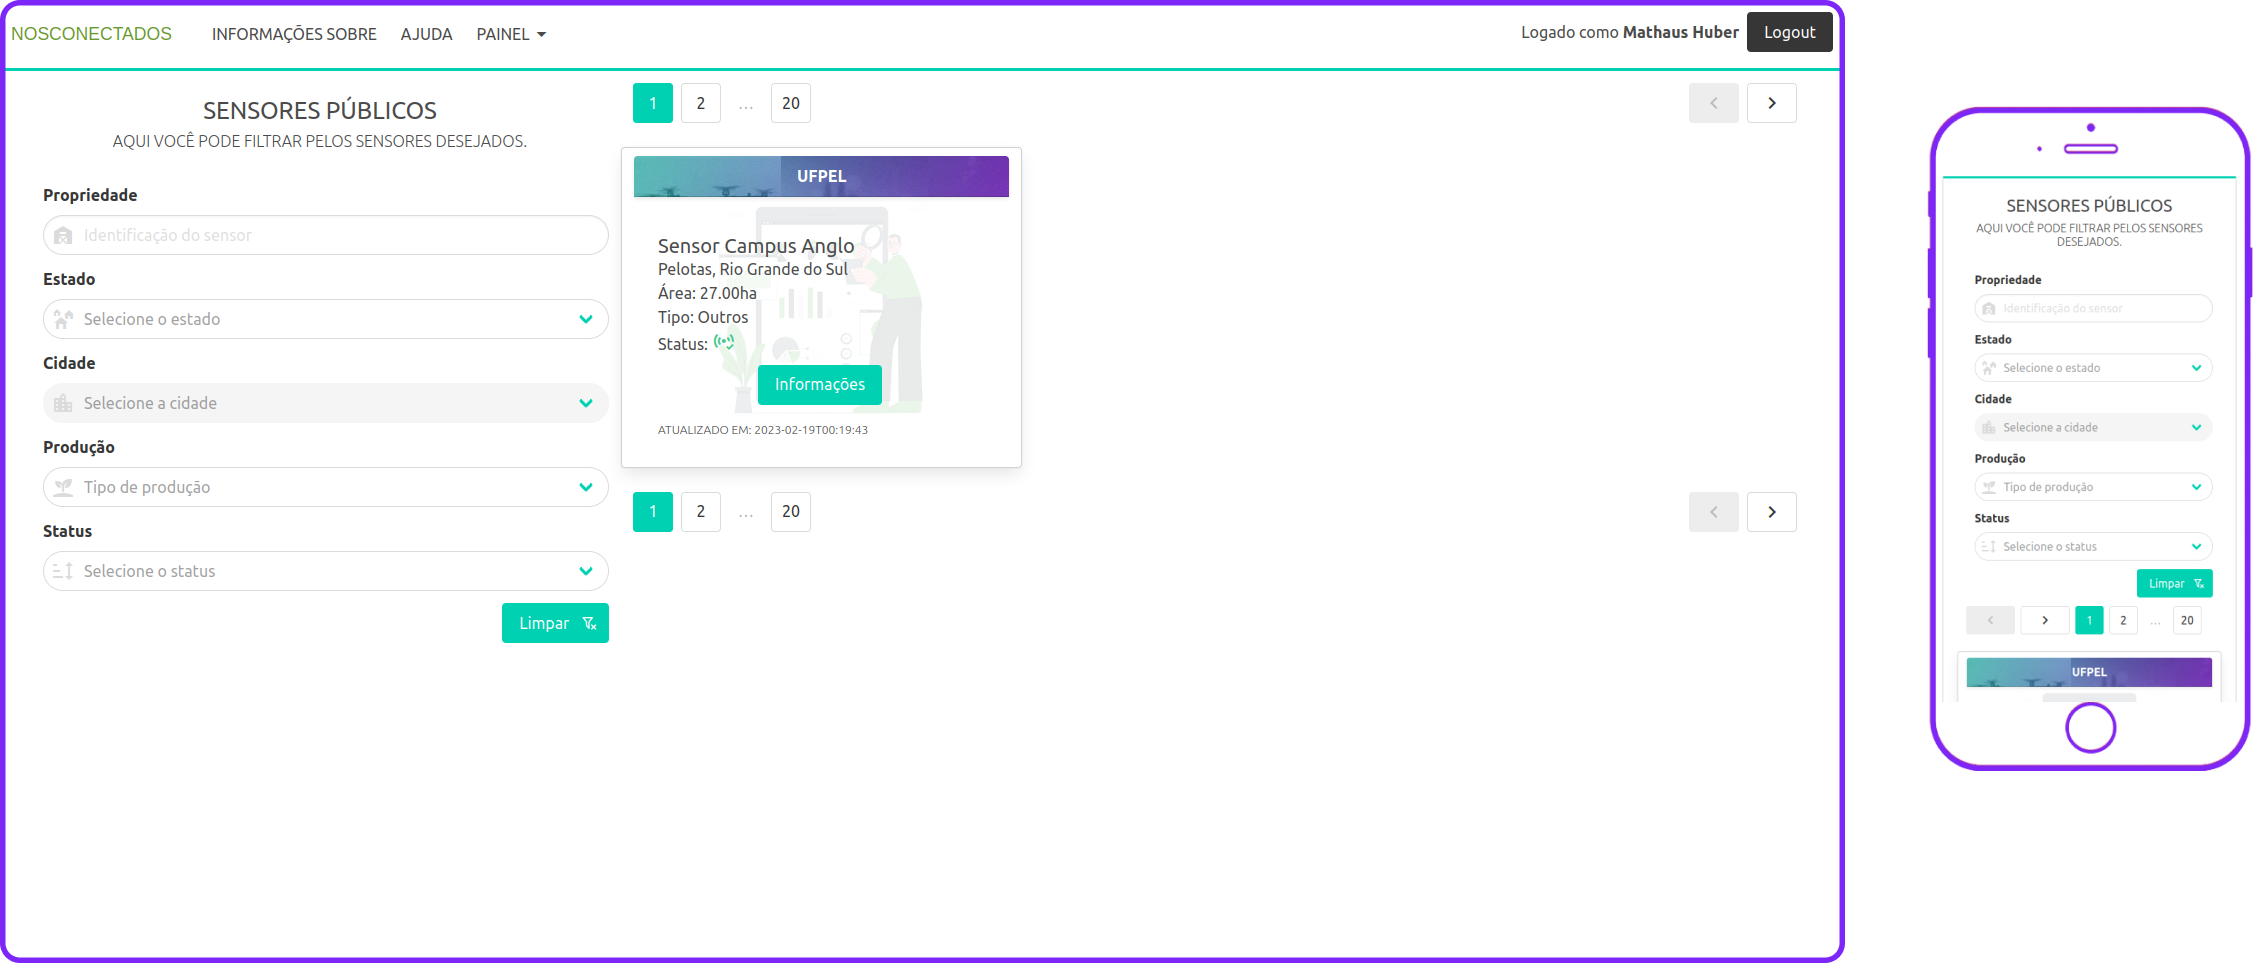
\includegraphics[scale=.2]{assets/sensorespublicos.png}
  \caption{Página de sensores públicos}
  \label{publicos}
\end{figure}

\begin{figure}[htbp]
  \centering 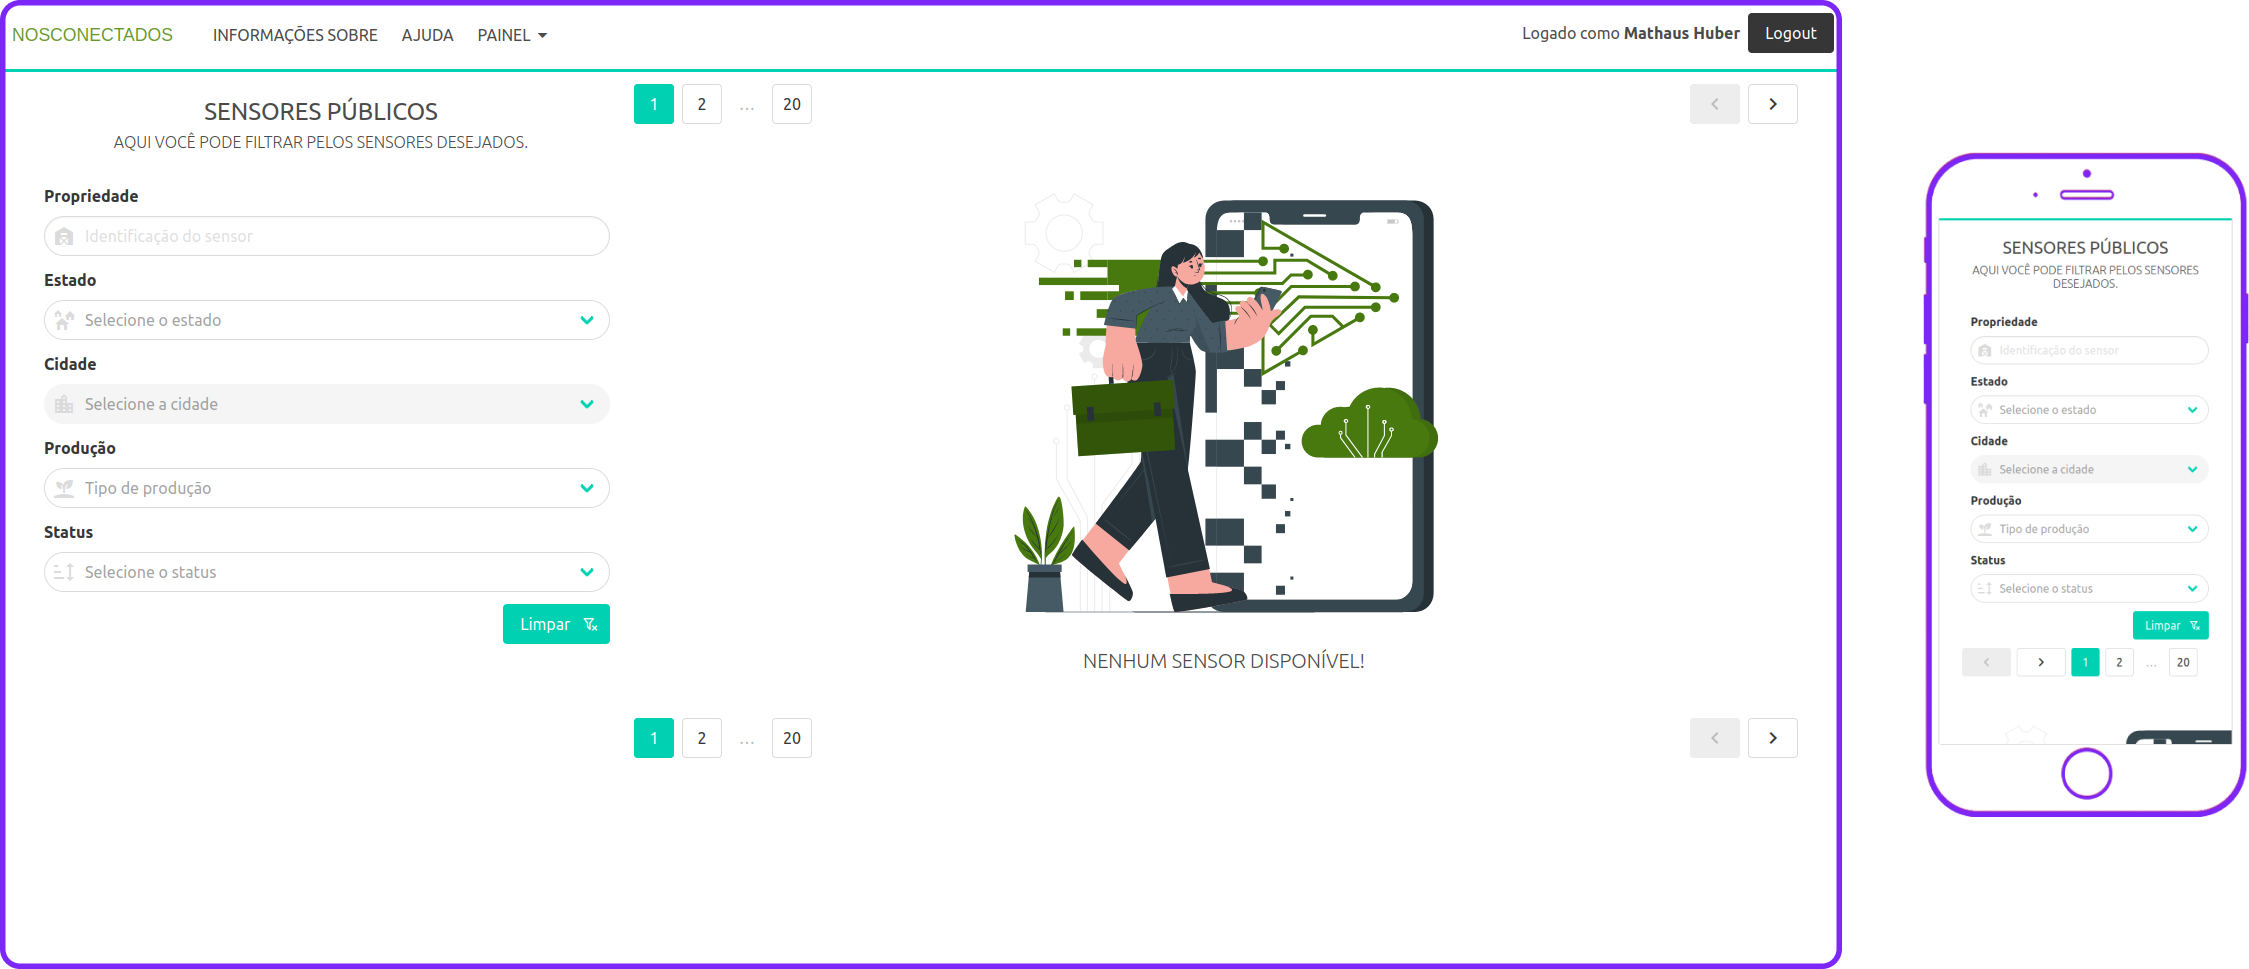
\includegraphics[scale=.2]{assets/sensorespublicosnull.png}
  \caption{Página de sensores públicos quando não há sensor público}
  \label{publicosnull}
\end{figure}
\newpage
\subsection{Ajuda}
\label{sec:paginaajuda}
A página de ajuda é uma seção importante na plataforma, pois oferece aos usuários informações e orientações úteis para entender como a plataforma funciona e como utilizar seus recursos. O manual disponível nesta página contém informações variadas, desde como inserir um sensor na plataforma até como funcionam os controles de usuários para aquele sensor. Essas informações são apresentadas de forma clara e detalhada para ajudar os usuários a entenderem melhor como a plataforma funciona.

Além disso, a página de ajuda também oferece informações sobre a geolocalização dentro da plataforma, permitindo aos usuários visualizar a localização geográfica dos sensores instalados. Essa funcionalidade é particularmente útil para usuários que desejam monitorar sensores em diferentes locais geográficos.
Outras informações que podem ser encontradas nesta seção incluem como visualizar solicitações para inserir sensores na plataforma, como se tornar um administrador, patrocinador ou visualizador de um sensor e como funciona o processo de inserção de novos usuários a determinados sensores.

Em resumo, a página de ajuda é uma seção crucial na plataforma, pois fornece informações importantes e orientações detalhadas para ajudar os usuários a utilizar a plataforma de forma eficiente e eficaz. Com esta seção, os usuários podem aprender como adicionar sensores, gerenciar usuários, e utilizar outras funcionalidades da plataforma, garantindo que eles possam aproveitar ao máximo seus recursos. Na figura \ref{ajuda} é possível ver como é a página de ajuda.
\begin{figure}[htbp]
  \centering 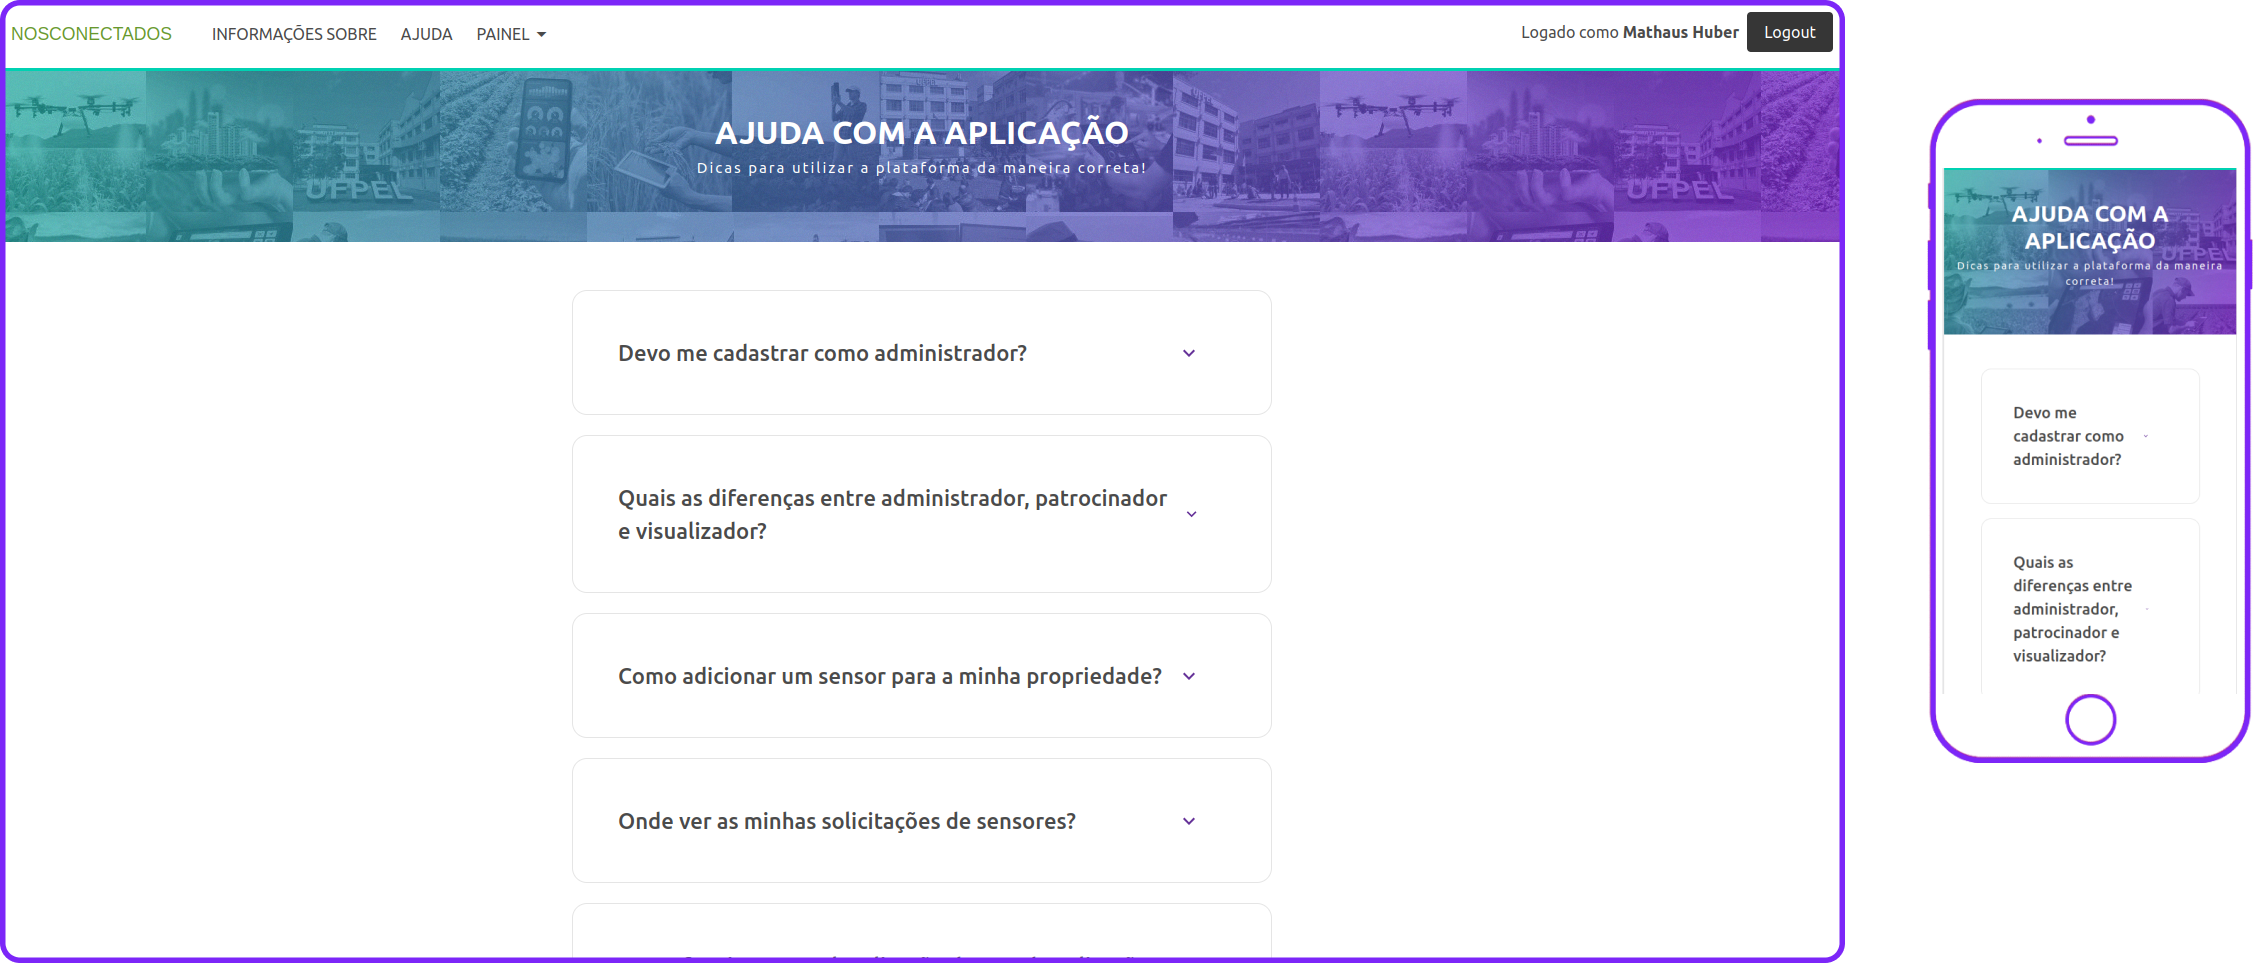
\includegraphics[scale=.2]{assets/ajuda.png}
  \caption{Página de ajuda}
  \label{ajuda}
\end{figure}
\newpage

\subsection{Cadastro de sensores}
A página de cadastro de sensores é uma das páginas mais importantes da plataforma, pois é onde os usuários podem criar novos sensores para serem monitorados pela rede de sensores sem fio. Para acessar essa página, o usuário precisa estar logado na plataforma, o que garante a segurança e a privacidade das informações dos sensores.

Ao acessar a página de cadastro de sensores, o usuário é apresentado a um formulário que deve ser preenchido com informações importantes sobre o novo sensor que será criado. Entre as informações necessárias estão a identificação da propriedade onde o sensor está localizado, o tipo de produção, a descrição do sensor, a área em hectares e o status (ativo ou inativo). Também é possível definir a privacidade do sensor, que pode ser público ou privado.

Além disso, o usuário precisa informar o estado e município onde o sensor está localizado, bem como a latitude e longitude do sensor. Para ajudar o usuário a encontrar a localização exata do sensor, a página conta com um botão de localização que usa a localização do usuário baseado no IP e, com permissão do usuário, traz a informação da sua localização atual no mapa.

Outra funcionalidade importante da página de cadastro de sensores é a possibilidade de adicionar administradores, patrocinadores e visualizadores para cada sensor. Isso permite que diferentes usuários tenham diferentes níveis de acesso aos sensores, o que é útil em situações onde é preciso compartilhar informações com outras pessoas ou organizações.

Em resumo, a página de cadastro de sensores é uma das principais funcionalidades da plataforma, permitindo que os usuários adicionem novos sensores e monitorem a rede de sensores sem fio de forma eficiente e segura. Na figura \ref{registro} é possível ver como é a página de cadastro de sensores.
\begin{figure}[htbp]
  \centering 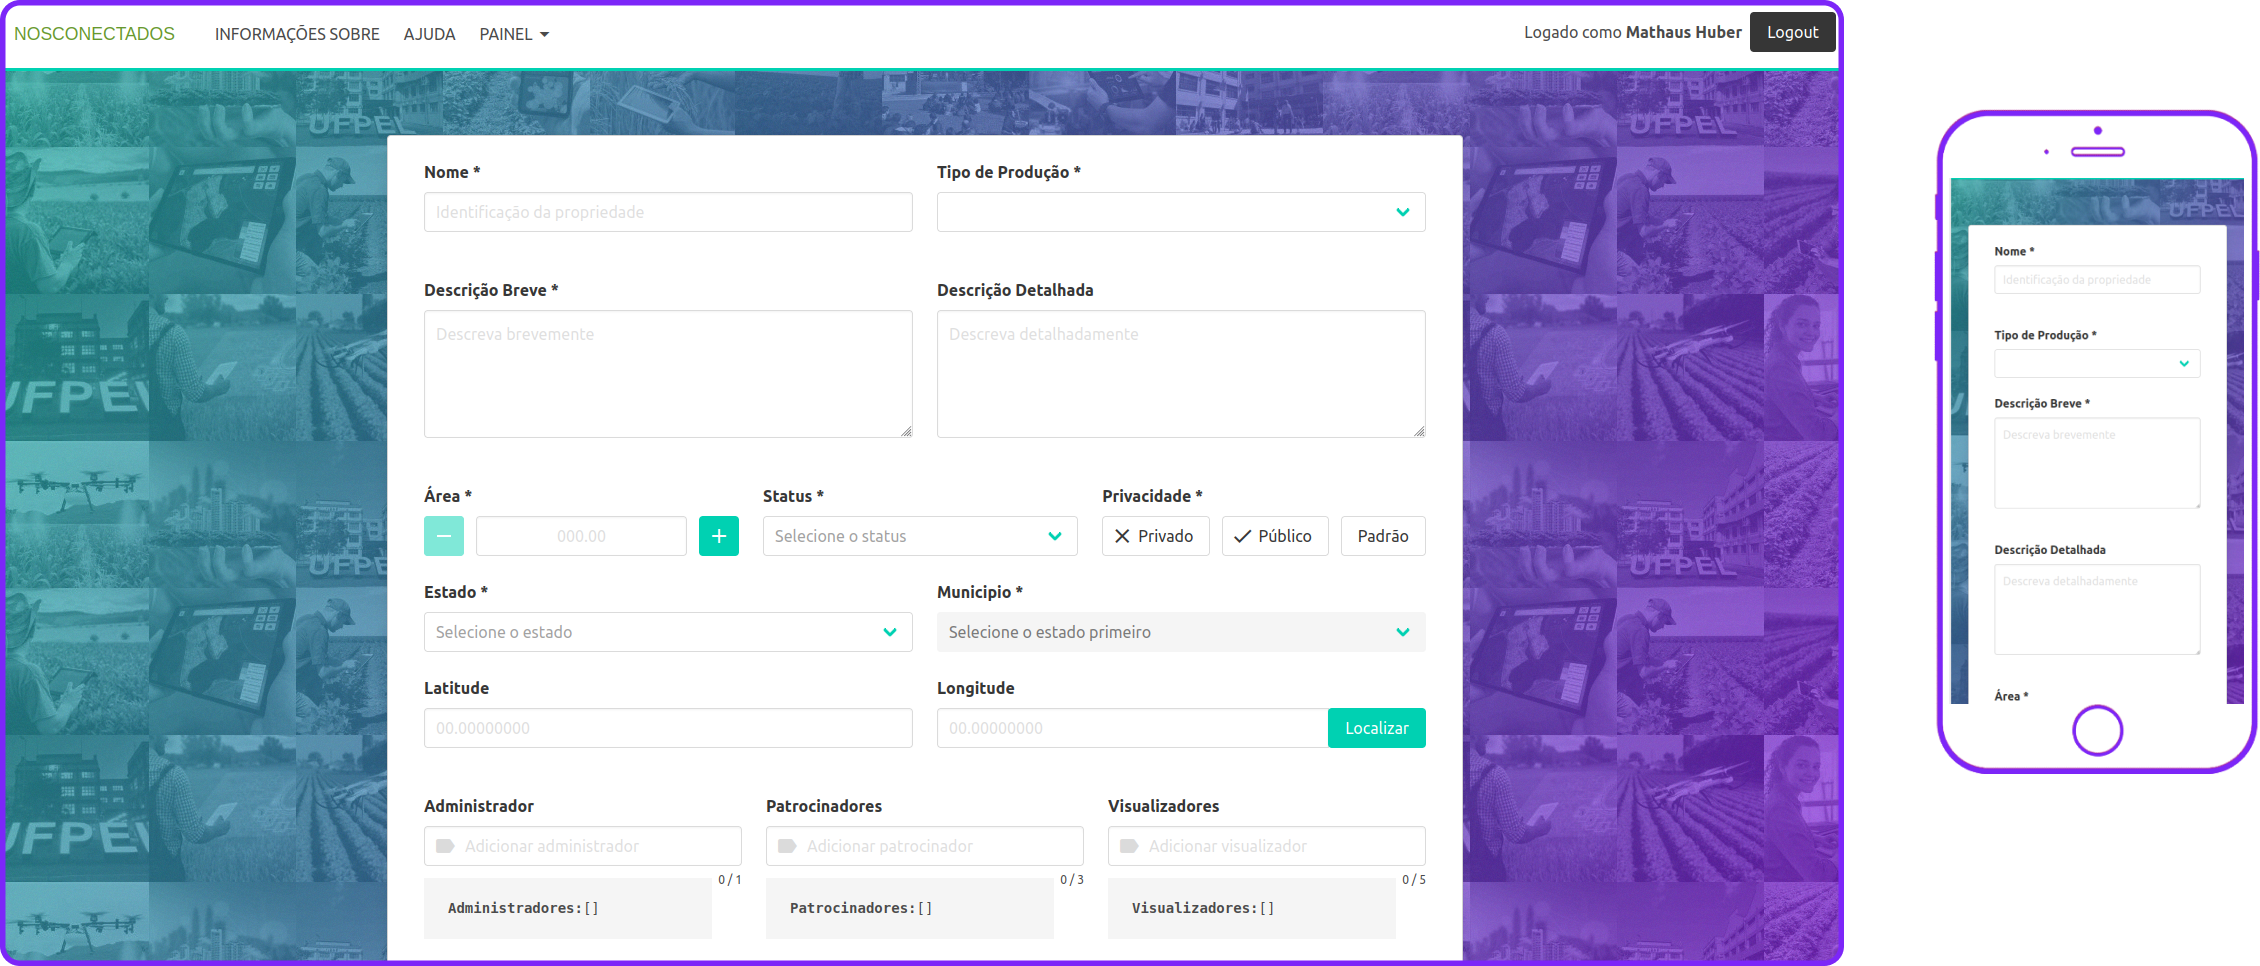
\includegraphics[scale=.2]{assets/cadastrosensores.png}
  \caption{Página de registro de sensores}
  \label{registro}
\end{figure}
\newpage

\subsection{Detalhes do sensor}
A página de detalhes do sensor é uma das mais importantes na plataforma, pois é nela que o usuário pode obter informações detalhadas sobre um determinado sensor. Na parte esquerda da página, são exibidas informações básicas sobre o sensor, como seu nome, localização, status, área e descrição. Essas informações permitem que o usuário identifique facilmente o sensor que está buscando.
Logo abaixo, são exibidos os dados atuais do sensor. Dados do sensor, como temperatura do solo, temperatura do ar, luminosidade, pluviometro e outros são apresentados de forma clara e concisa. Isso permite que o usuário visualize rapidamente as informações mais importantes do sensor.

Na parte direita da página, ficam os gráficos que mostram as séries históricas do sensor. Esses gráficos permitem que o usuário veja a história dos dados do sensor em formato de dashboards, tornando mais fácil a visualização e análise dos dados. Geralmente, são apresentados três gráficos principais: um que mostra informações de temperatura, outro que mostra informações do tempo e um terceiro que mostra informações da atmosfera. Esses gráficos permitem que o usuário visualize a evolução dos dados ao longo do tempo e identifique possíveis tendências ou padrões.

Em suma, a página de detalhes do sensor é uma ferramenta importante para que o usuário possa acessar e analisar informações detalhadas sobre um sensor específico. Isso permite que ele tome decisões mais informadas com base nos dados obtidos e possa monitorar de forma eficiente a rede de sensores sem fio.  Na figura \ref{detalhes} é possível ver como é a página de detalhes do sensor.
\begin{figure}[htbp]
  \centering 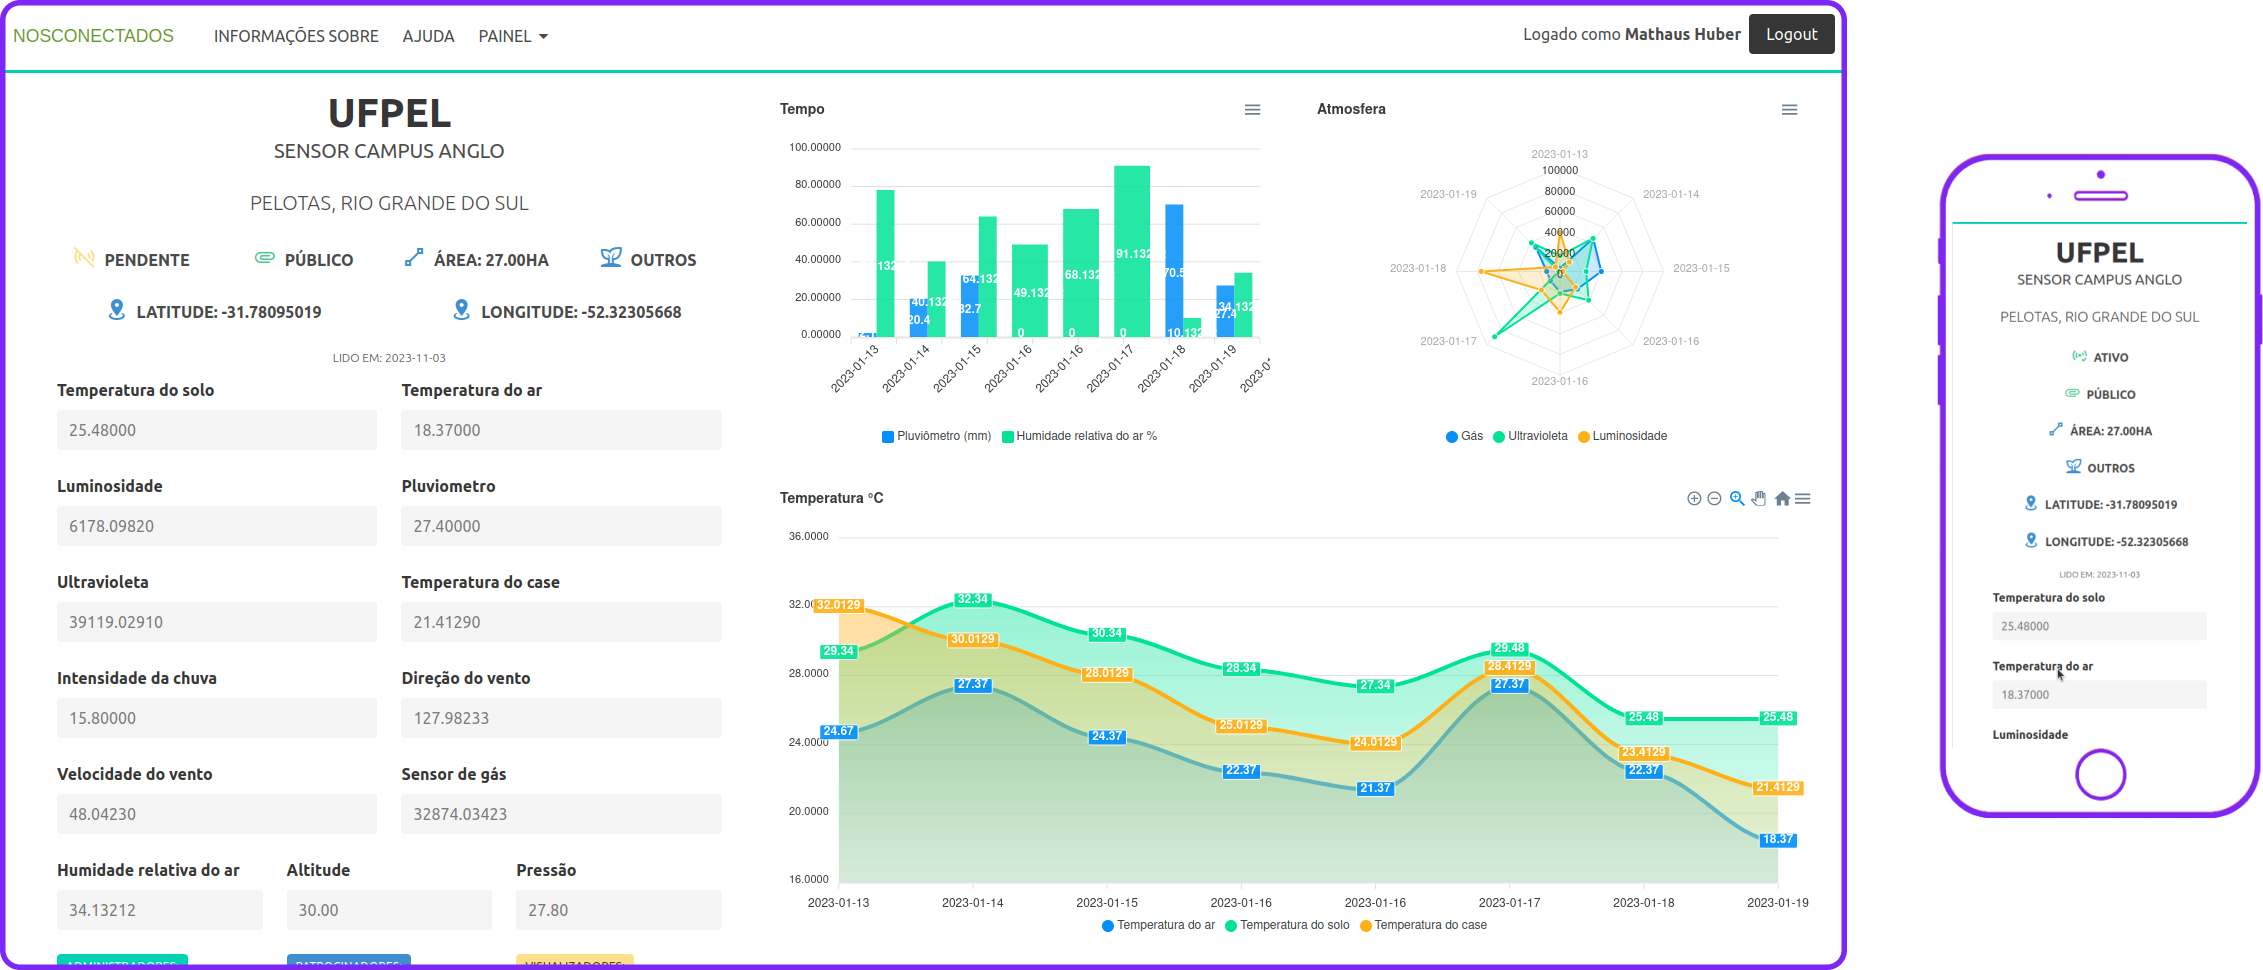
\includegraphics[scale=.2]{assets/detalhes.png}
  \caption{Página de detalhes do sensor}
  \label{detalhes}
\end{figure}
\newpage
\subsection{Editar perfil}
A página de editar perfil permite que o usuário atualize suas informações pessoais. Para acessá-la, o usuário precisa estar logado e clicar na opção "Editar perfil" que fica na barra de navegação.
Ao acessar a página, o usuário verá um formulário com as informações pessoais dele, como nome completo, e-mail, telefone, endereço, entre outras informações que ele preencheu durante o cadastro. Além disso, o formulário também contém informações adicionais, como a senha e a imagem do perfil.

Ao editar as informações, o usuário pode atualizar sua senha, trocar a foto do perfil e modificar outros detalhes de contato, como o número de telefone ou endereço de e-mail. Isso ajuda a garantir que a plataforma esteja sempre atualizada com as informações mais recentes do usuário.

Em resumo, a página de editar perfil é uma parte crítica da plataforma, pois permite que os usuários atualizem suas informações pessoais e personalizem a experiência da plataforma de acordo com suas necessidades e preferências. Na figura \ref{editperfil} é possível ver como é a página de edição de perfil.
\begin{figure}[htbp]
  \centering 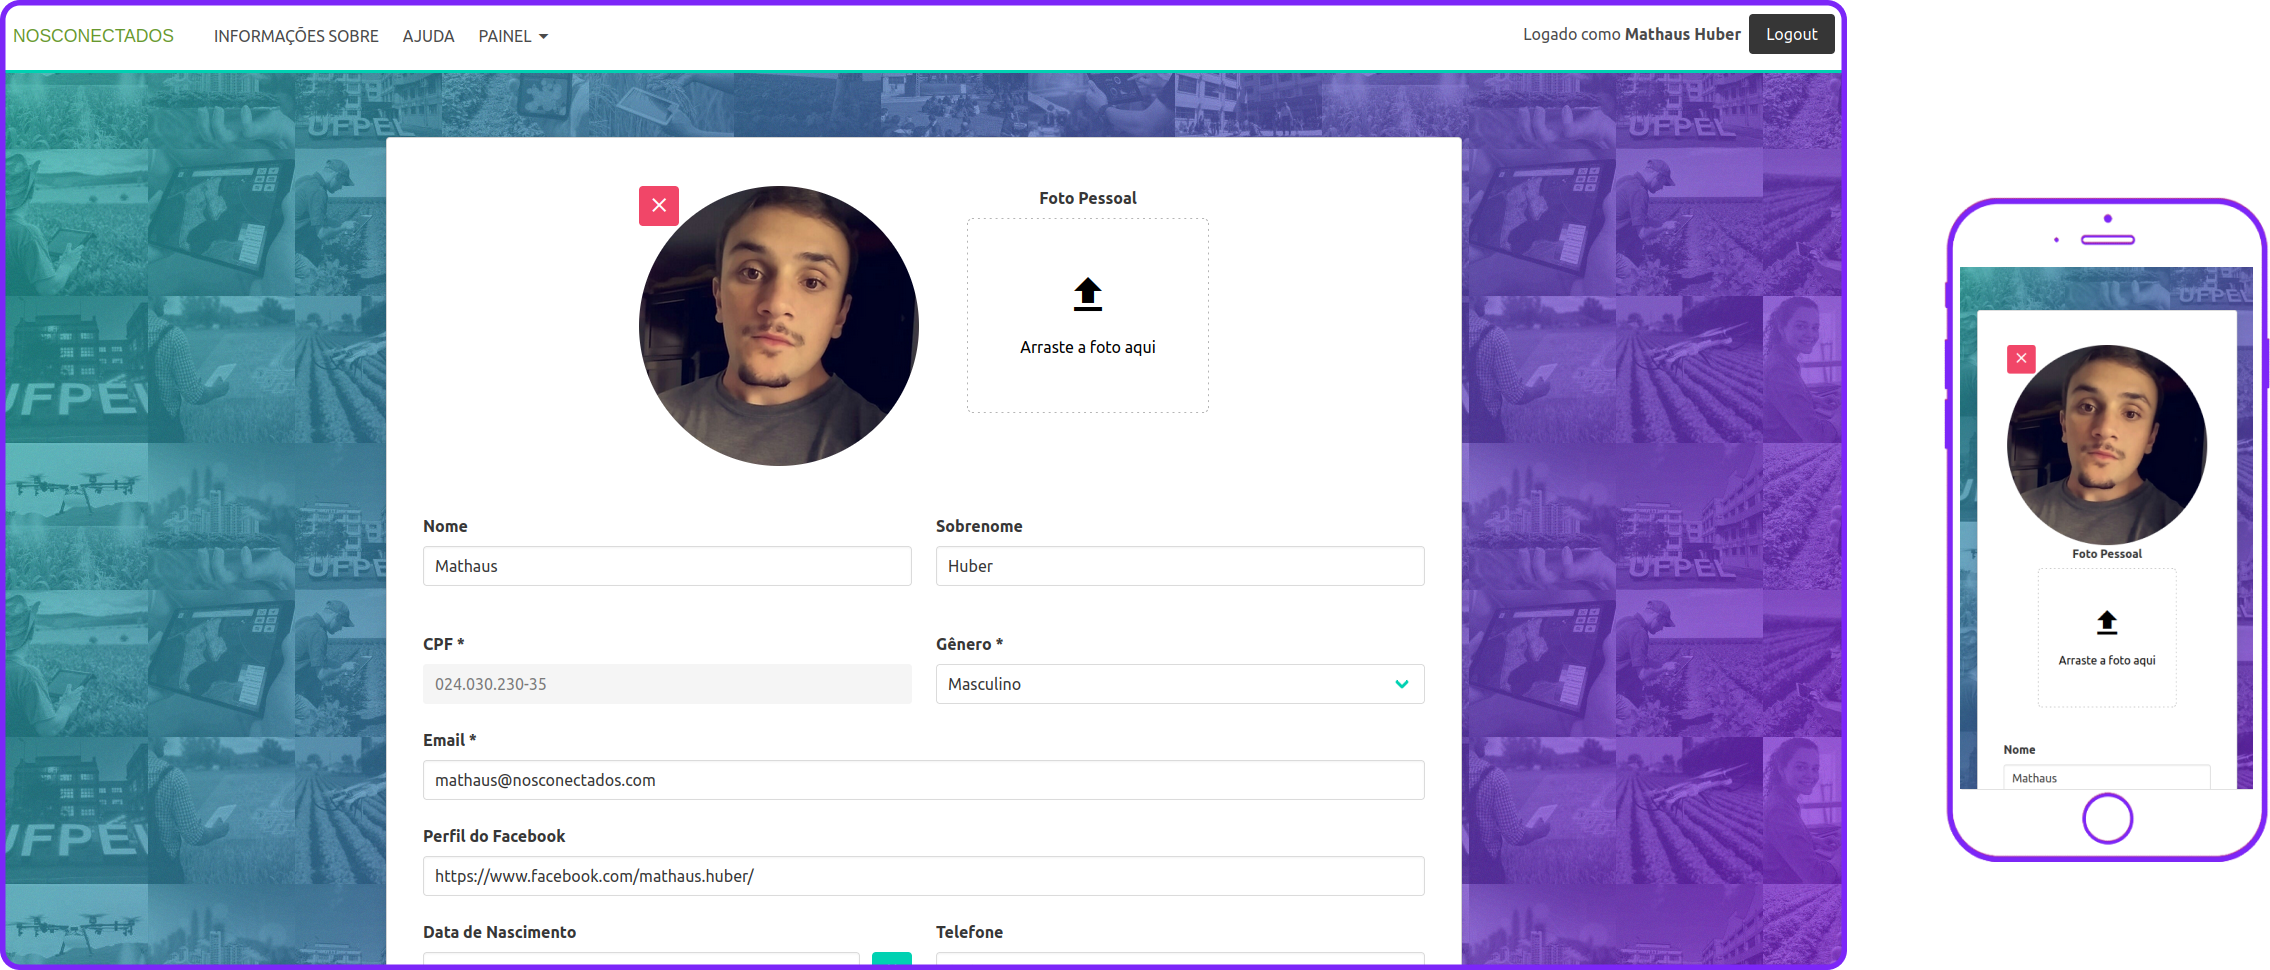
\includegraphics[scale=.2]{assets/editarperfil.png}
  \caption{Página de edição de perfil do usuário}
  \label{editperfil}
\end{figure}
\newpage
\subsection{Editar sensor}
Na página de edição de sensor, o usuário pode atualizar todas as informações relacionadas ao sensor, incluindo seu nome, descrição, localização, tipo, status e outras propriedades relevantes. Além disso, o usuário pode editar a lista de patrocinadores e visualizadores do sensor, permitindo que outras pessoas também possam ter acesso aos dados coletados por ele.

É importante ressaltar que apenas usuários autenticados e autorizados podem acessar essa página, já que ela contém informações sensíveis e importantes para a plataforma. Além disso, os administradores não podem ser modificados após a inserção, o que ajuda a garantir a integridade e segurança dos dados coletados pelo sensor.

Portanto, a página de edição de sensor é uma ferramenta muito importante para o gerenciamento da plataforma, permitindo que o usuário tenha total controle sobre as informações dos sensores cadastrados e garanta que os dados estejam sempre atualizados e seguros. Na figura \ref{editsensor} é possível ver como é a página de edição de sensores.

\begin{figure}[htbp]
  \centering 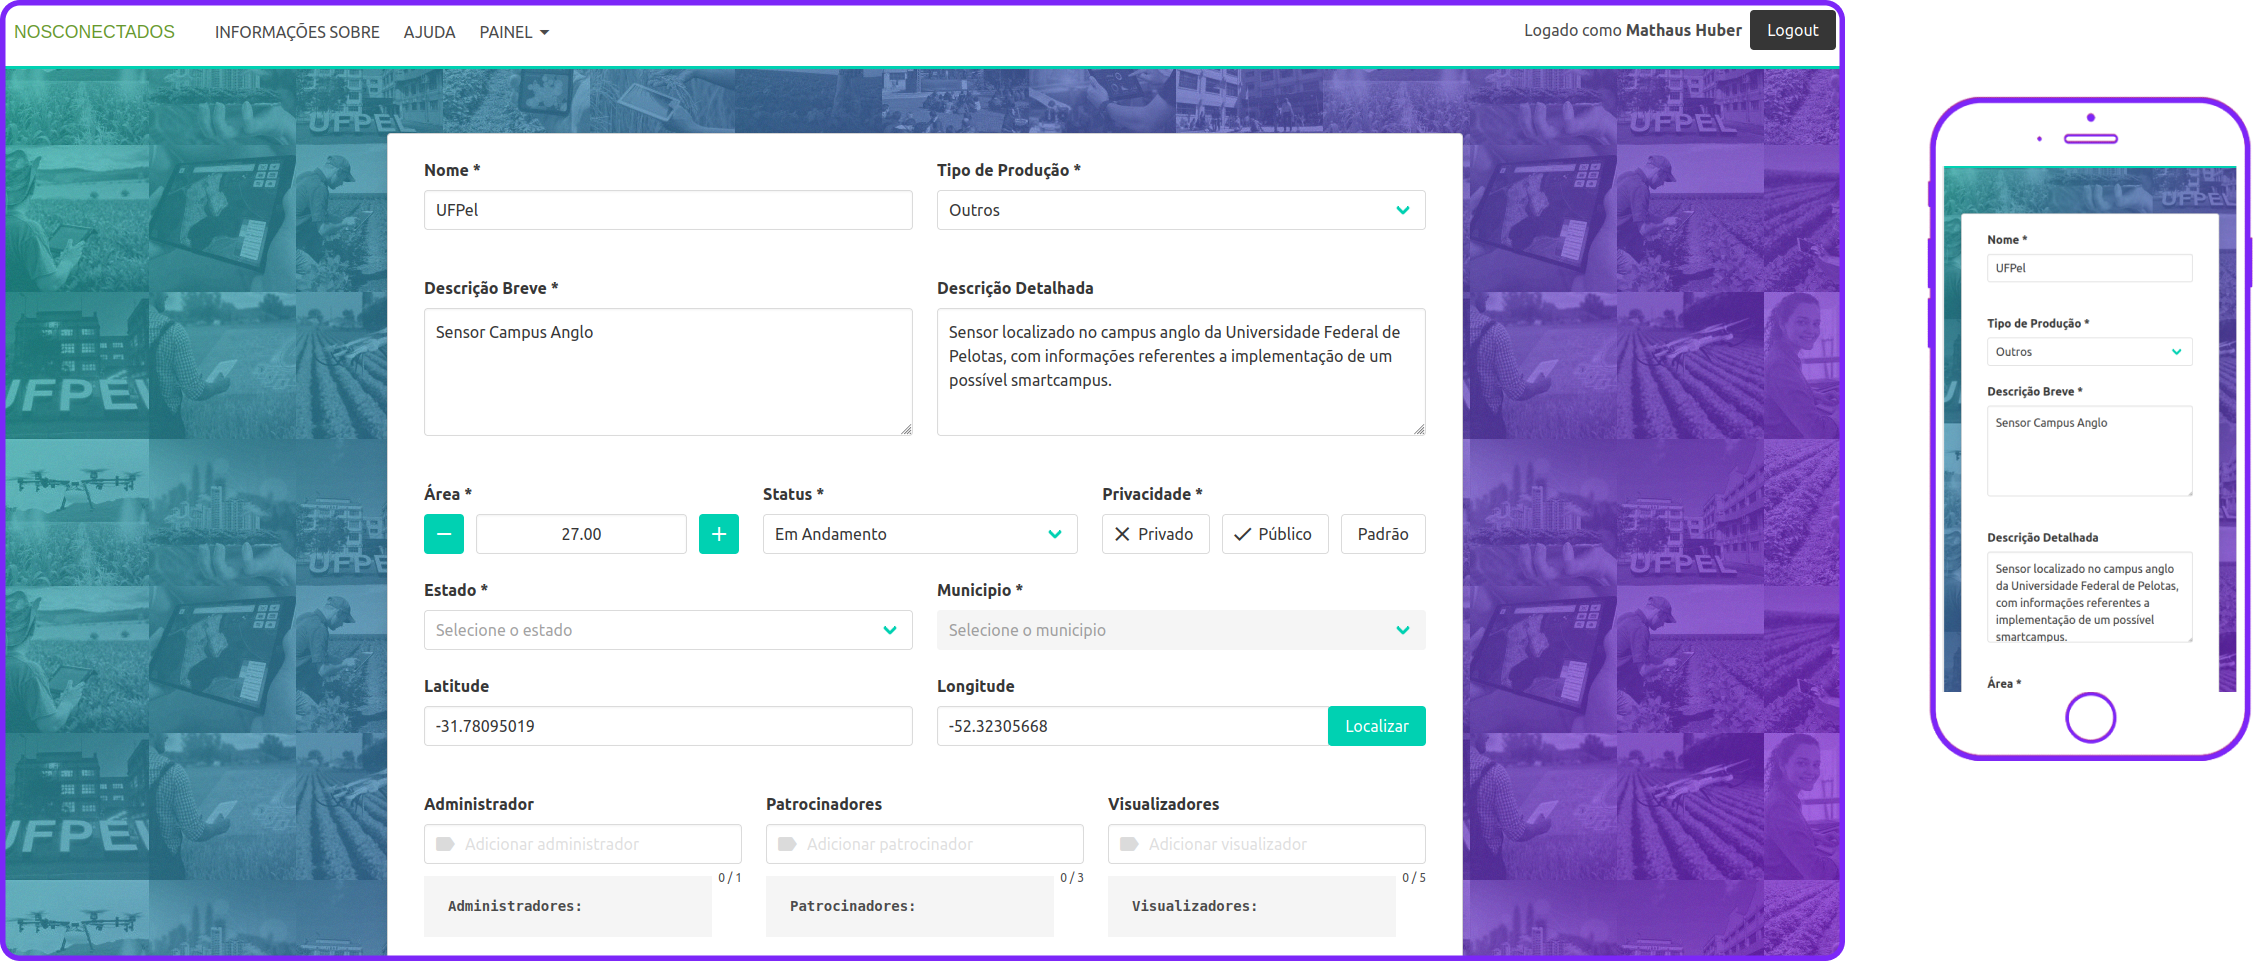
\includegraphics[scale=.2]{assets/editarsensor.png}
  \caption{Página de edição de sensores}
  \label{editsensor}
\end{figure}
\newpage
\subsection{Sensores solicitados}
A página de sensores solicitados é onde o usuário pode gerenciar as solicitações de sensores que foram feitas. Na esquerda da página, o usuário pode filtrar as solicitações de sensores com base em diferentes critérios, como nome da propriedade, estado, cidade, tipo de produção e status do sensor. Na parte direita da página, são exibidos os sensores solicitados que correspondem aos critérios de filtro escolhidos. Cada sensor solicitado é exibido em um card com informações como o nome da propriedade, localização e tipo de produção.


Além disso, há um botão no meio do card de cada sensor que leva o usuário para a página de atribuição de sensor. Nesta página, o usuário pode atribuir o sensor solicitado a um sensor instalado na propriedade, permitindo que ele comece a coletar dados.

A página de sensores solicitados é uma seção crucial para a plataforma, pois, permite que os usuários vejam as suas solicitações e possam atribuir os sensores que foram criados na plataforma a um sensor instalado. Com a capacidade de filtrar e atribuir solicitações de sensores, a plataforma é capaz de se adaptar às necessidades dos usuários e fornecer informações valiosas para a tomada de decisões em diferentes setores. A página que exibe os sensores solicitados pelos usuários pode ser vista na figura \ref{solicitados}. Caso não haja nenhuma solicitação de sensor pendente, uma mensagem é exibida ao usuário na página, como pode ser observado na figura \ref{solicitadosnull}.

\begin{figure}[htbp]
  \centering 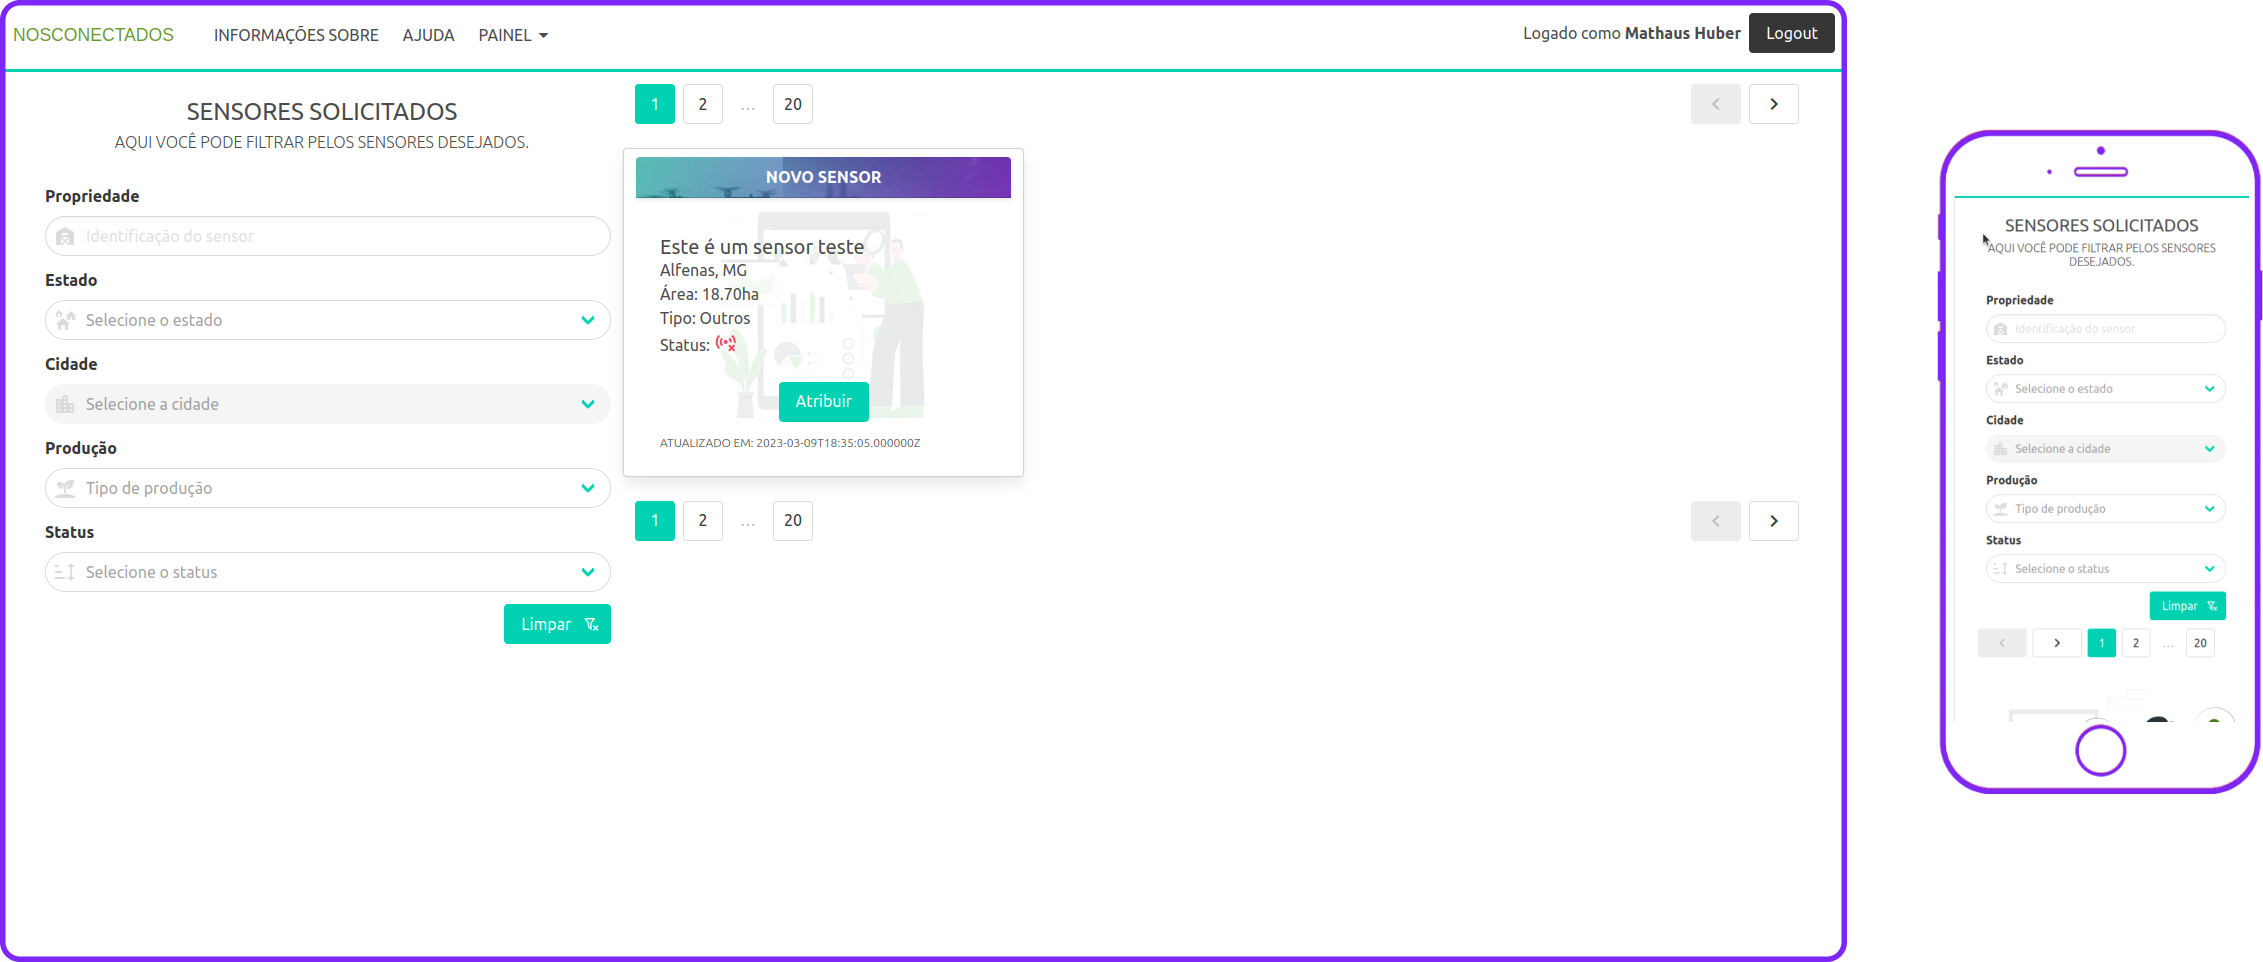
\includegraphics[scale=.2]{assets/solicitados.png}
  \caption{Página de sensores solicitados}
  \label{solicitados}
\end{figure}

\begin{figure}[htbp]
  \centering 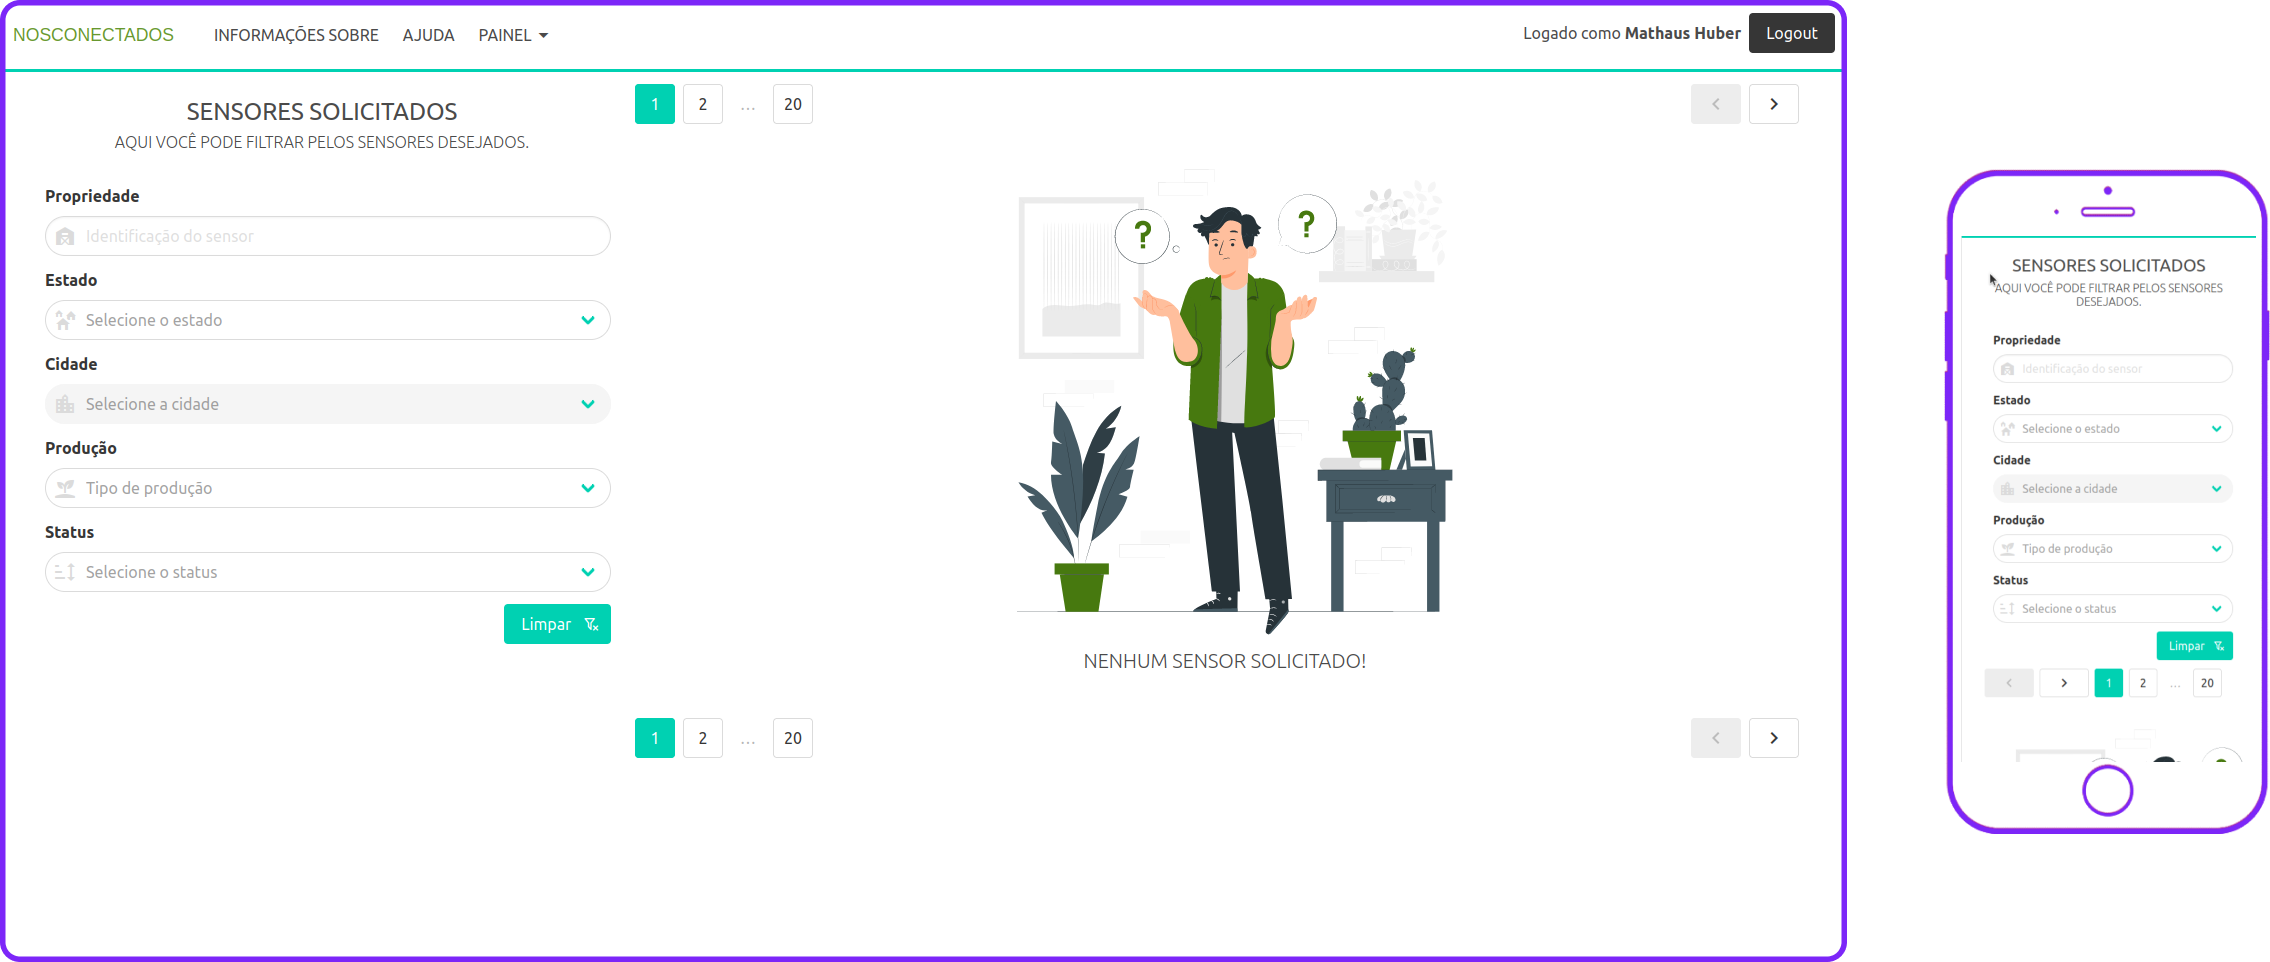
\includegraphics[scale=.2]{assets/solicitadosnull.png}
  \caption{Página de sensores solicitados quando não há solicitação}
  \label{solicitadosnull}
\end{figure}
\newpage
\subsection{Sobre}
A página de informações sobre é o local onde os usuários podem encontrar informações importantes sobre a plataforma e entender melhor sua proposta. Ao acessar a página, o usuário é recebido com uma frase impactante que resume a essência da plataforma: "TECNOLOGIA ALIADA A INOVAÇÃO! Soluções estruturadas em auxílio a tomada de decisão com base no uso de Redes de Sensores sem Fio aplicadas a smartfarms, smartcities e smartcampus."\space A imagem que acompanha essa frase transmite modernidade e tecnologia, reforçando a proposta da plataforma.

A segunda seção da página contém informações mais detalhadas sobre a plataforma, abordando questões como: quem somos, o que oferecemos e qual é o intuito por trás da criação do sistema. Essas informações são relevantes e ajudam o usuário a compreender melhor a nossa proposta e a decidir se ela atende às suas necessidades.

Por fim, a terceira seção da página é dedicada a um formulário de avaliação da plataforma, onde os usuários podem deixar seus comentários e sugestões sobre a plataforma. Essa seção é importante para o desenvolvimento contínuo da plataforma, pois permite que os desenvolvedores recebam feedback direto dos usuários e melhorem a plataforma com base nessas informações.

Em resumo, a página de informações sobre é uma seção crucial da plataforma, pois ajuda os usuários a entender melhor sua proposta e oferece uma oportunidade para eles deixarem feedback direto sobre a plataforma. Com isso, a plataforma pode continuar evoluindo e se adaptando às necessidades dos usuários, oferecendo soluções cada vez mais eficientes e inovadoras. A página de informações sobre possui três seções distintas. A primeira seção pode ser visualizada na figura \ref{sobre-1}, a segunda na figura \ref{sobre-2} e a terceira seção na figura \ref{sobre-3}.
\begin{figure}[htbp]
  \centering 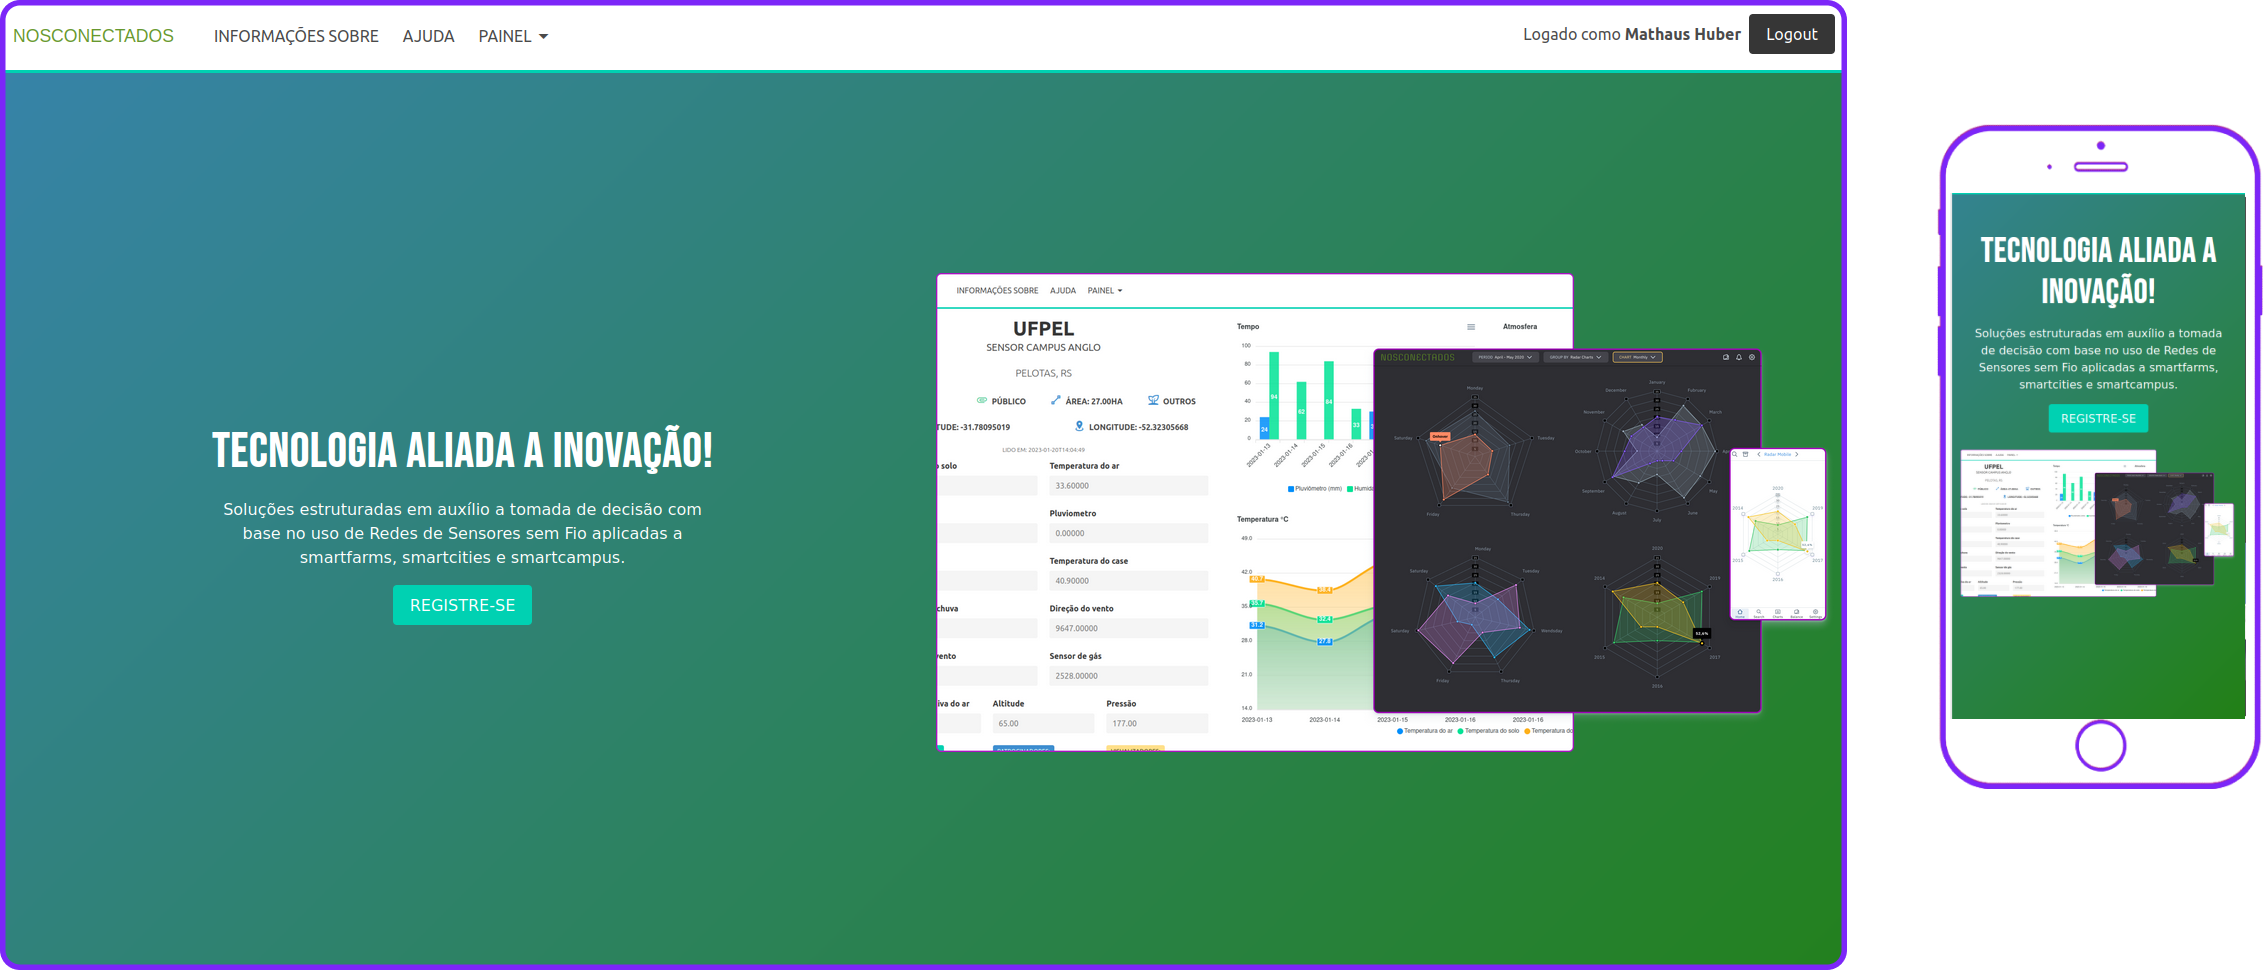
\includegraphics[scale=.2]{assets/sobre1.png}
  \caption{Página de informações sobre a plataforma - primeira seção}
  \label{sobre-1}
\end{figure}

\begin{figure}[htbp]
  \centering 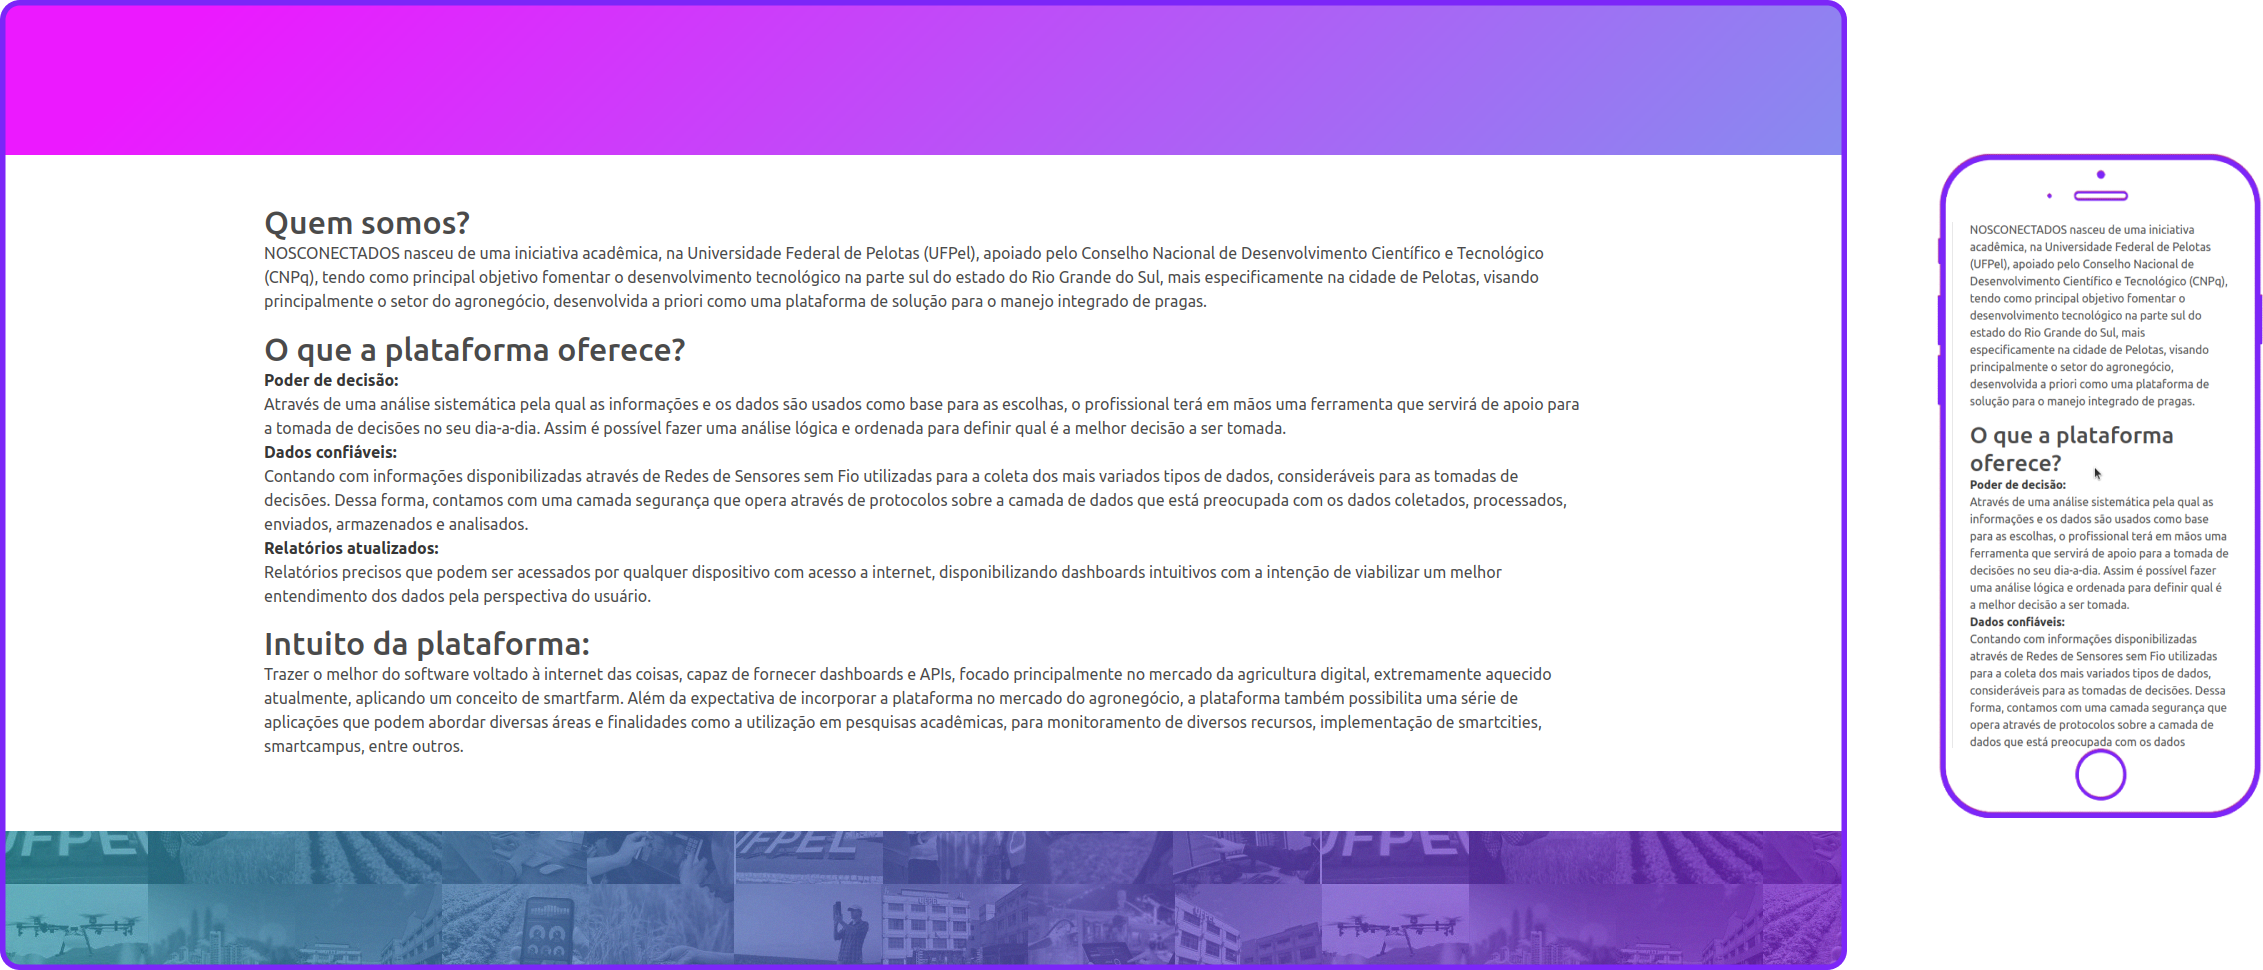
\includegraphics[scale=.2]{assets/sobre2.png}
  \caption{Página de informações sobre a plataforma - segunda seção}
  \label{sobre-2}
\end{figure}

\begin{figure}[htbp]
  \centering 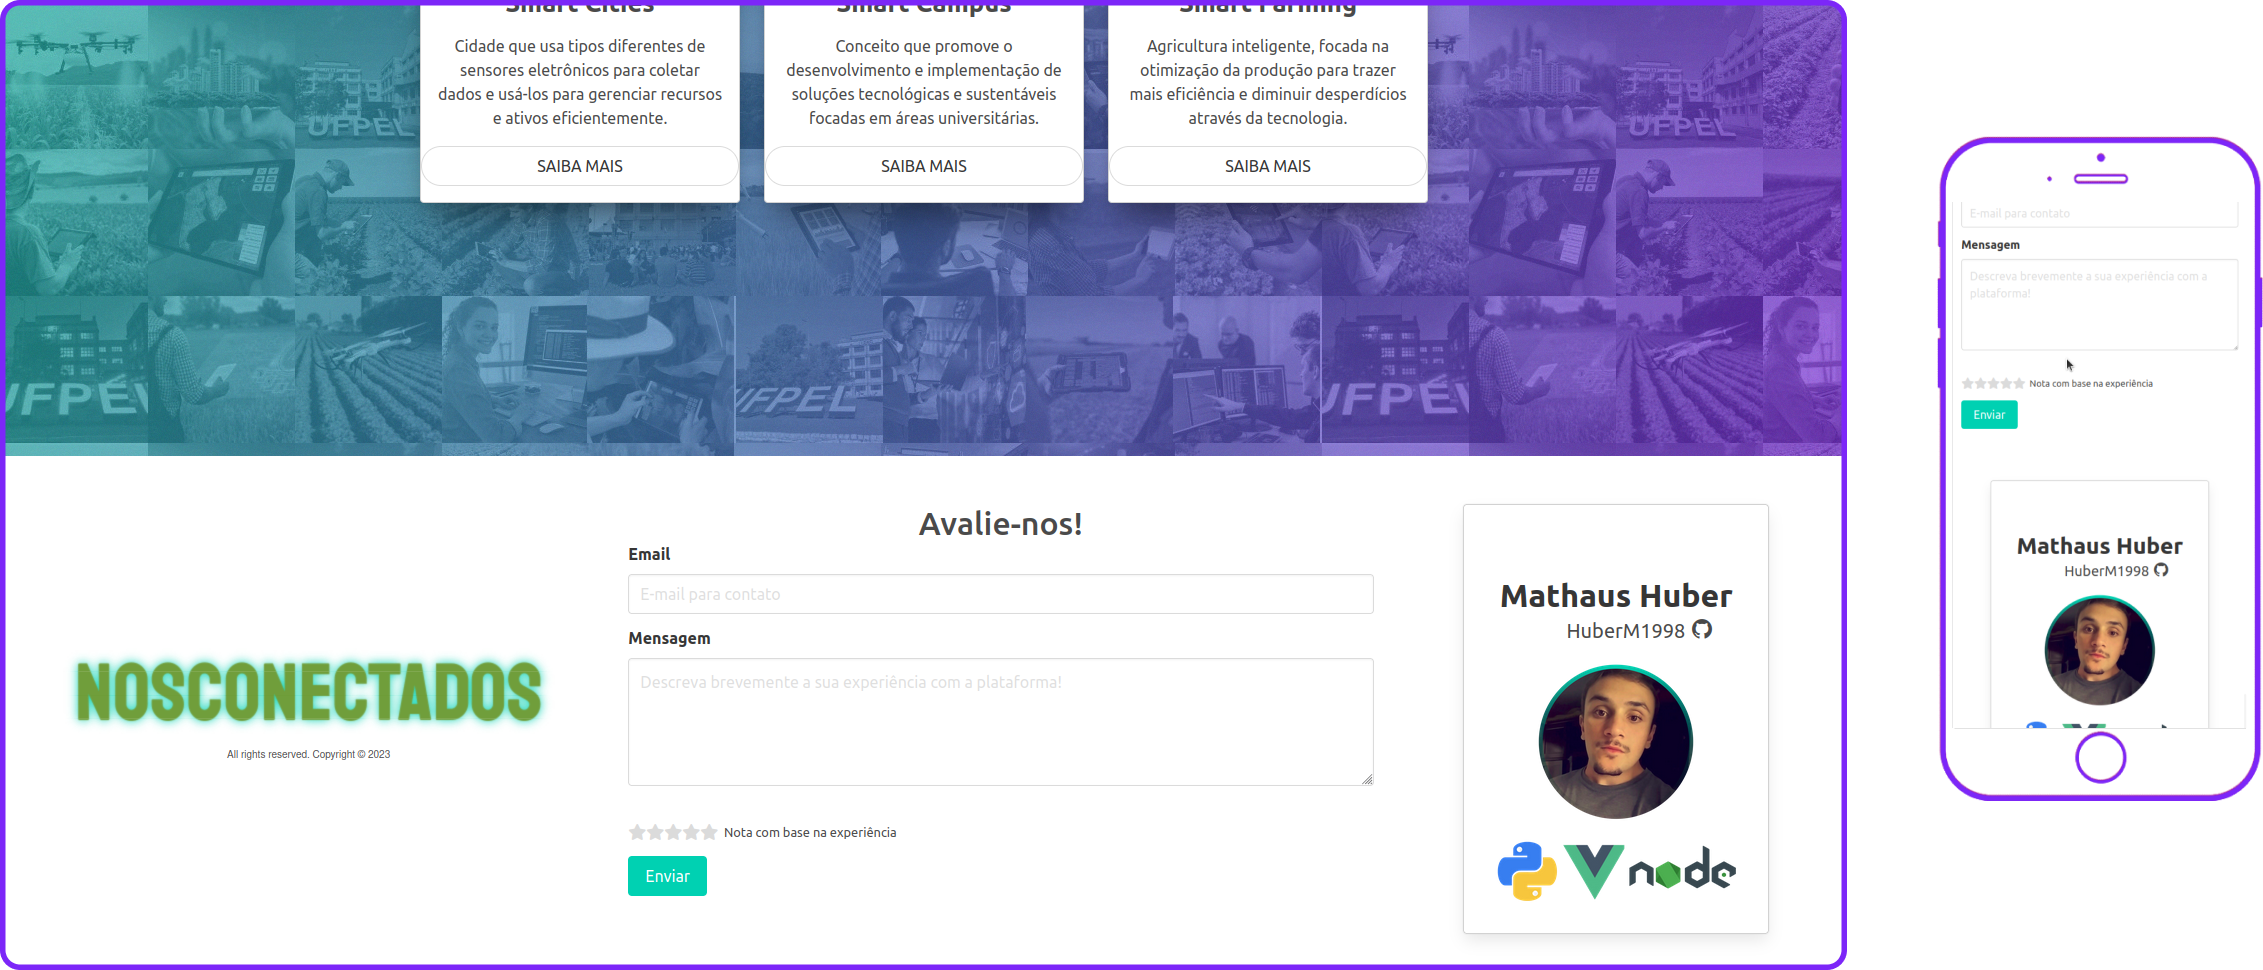
\includegraphics[scale=.2]{assets/sobre3.png}
  \caption{Página de informações sobre a plataforma - terceira seção}
  \label{sobre-3}
\end{figure}
\newpage
\subsection{Atribuição de sensores}
A página de atribuição de sensores é uma das funcionalidades principais da plataforma, pois é nela que os usuários podem vincular os sensores que desejam monitorar à plataforma. A página é acessível apenas para usuários autenticados, garantindo a segurança e privacidade das informações.

Ao clicar no botão "Atribuir" \space na página de sensores solicitados, o usuário é direcionado para a página de atribuição. Na página de atribuição, o usuário tem a opção de selecionar um sensor já instalado e em funcionamento para vincular à plataforma ou gerar um token para um sensor que ainda será instalado.

Se o usuário selecionar um sensor já instalado, ele pode ver uma lista de sensores disponíveis e escolher o que deseja vincular à plataforma. É importante notar que apenas sensores compatíveis com a plataforma e que estão referenciados àquele usuário são exibidos nessa lista. Caso o usuário deseje vincular um sensor que ainda não está em funcionamento, ele pode gerar um token exclusivo na plataforma. Esse token será utilizado para identificar o sensor quando ele for instalado e começar a enviar dados para a plataforma. Assim, o usuário poderá monitorar os dados coletados por esse sensor.


Em resumo, a página de atribuição de sensores é uma ferramenta importante para que os usuários possam monitorar os dados de sensores instalados em suas propriedades. Com ela, é possível vincular sensores já em funcionamento ou gerar tokens exclusivos para sensores que serão instalados no futuro. Na figura \ref{atribuicao} como é a página de atribuição de sensores.

\begin{figure}[htbp]
  \centering 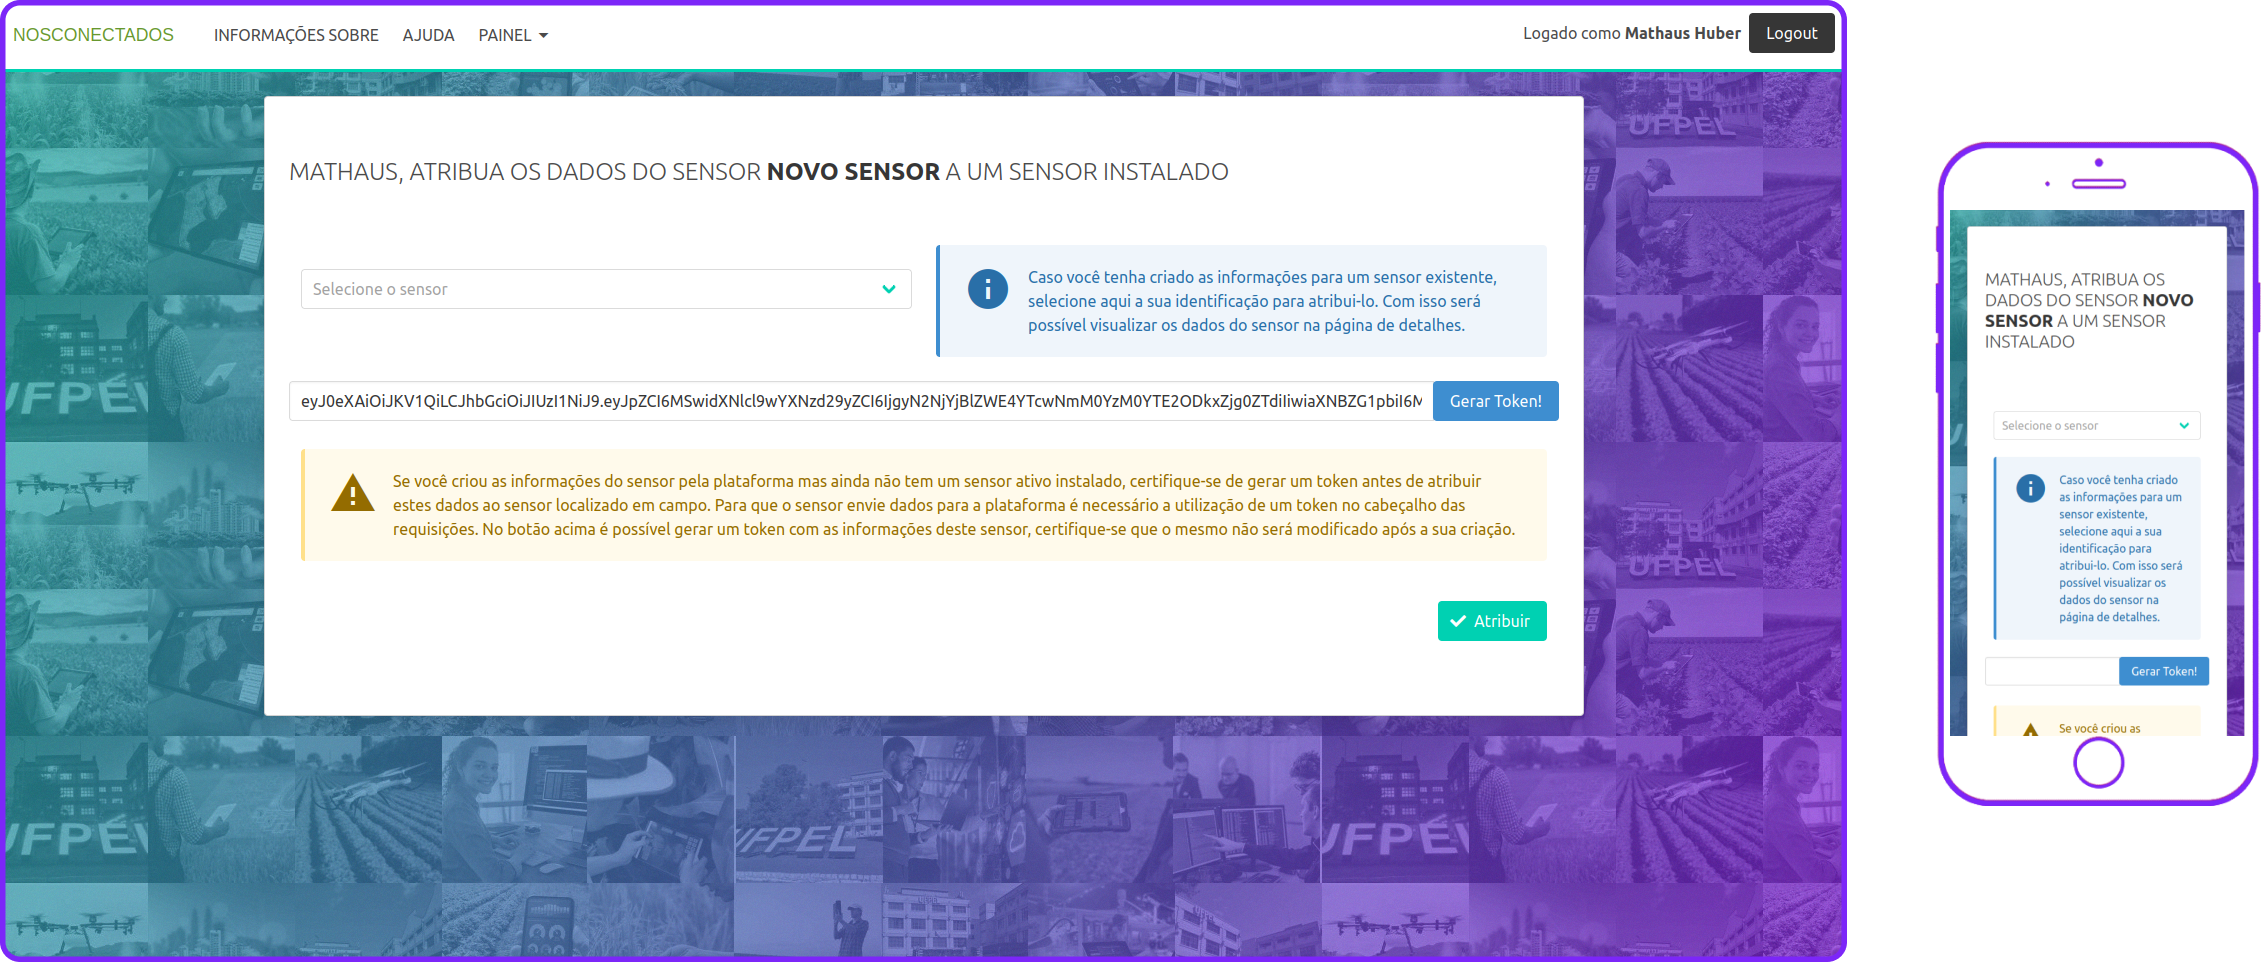
\includegraphics[scale=.2]{assets/atribuicao.png}
  \caption{Página de atribuição de sensores}
  \label{atribuicao}
\end{figure}
\newpage
\subsection{Sensores do usuário}
A página de sensores do usuário é uma das páginas mais importantes da plataforma, pois é nela que o usuário pode gerenciar os seus próprios sensores. Ela oferece uma interface amigável e intuitiva, permitindo que o usuário filtre e visualize os sensores instalados em suas propriedades.

Na lateral esquerda da página, há uma seção de filtros que permite ao usuário buscar pelos sensores desejados, utilizando critérios como o nome da propriedade onde o sensor está instalado, estado, cidade, tipo de produção e status do sensor. Ao aplicar os filtros, a página é atualizada com os resultados correspondentes.

Ao lado direito da página, são mostrados os sensores que atendem aos critérios de filtro. Cada sensor é apresentado em um card contendo informações como o nome da propriedade, o tipo de sensor, a data de instalação, o status (ativo, inativo ou pendente) e a última leitura registrada. No final de cada card, há três botões para acessar a página de detalhes do sensor, a página de edição e a opção de remover o sensor.

Na página de detalhes do sensor, o usuário pode visualizar informações mais detalhadas sobre o sensor, como os dados atuais gerados por aquele sensor, as séries históricas em formato de dashboard e as informações de localização. Já na página de edição, é possível fazer alterações nas informações do sensor, como o nome da propriedade, a localização e o acesso aos usuários. Por fim, a opção de remover o sensor permite ao usuário excluir um sensor da plataforma, caso esse usuário seja um administrador.


Essa página é essencial para o gerenciamento dos sensores do usuário, permitindo que ele tenha um controle mais eficiente sobre as informações coletadas pelos seus dispositivos de monitoramento. Na figura \ref{meusensores} é possível ver como é a página de sensores do usuário. A página de sensores do usuário pode ser visualizada na figura \ref{meusensores}. Na figura \ref{meusensoresnull}, é possível ver como a página é exibida quando não há sensores registrados pelo usuário. Caso o usuário deseje remover um sensor, a página correspondente pode ser vista na figura \ref{meusensoresremove}. 
\begin{figure}[htbp]
  \centering 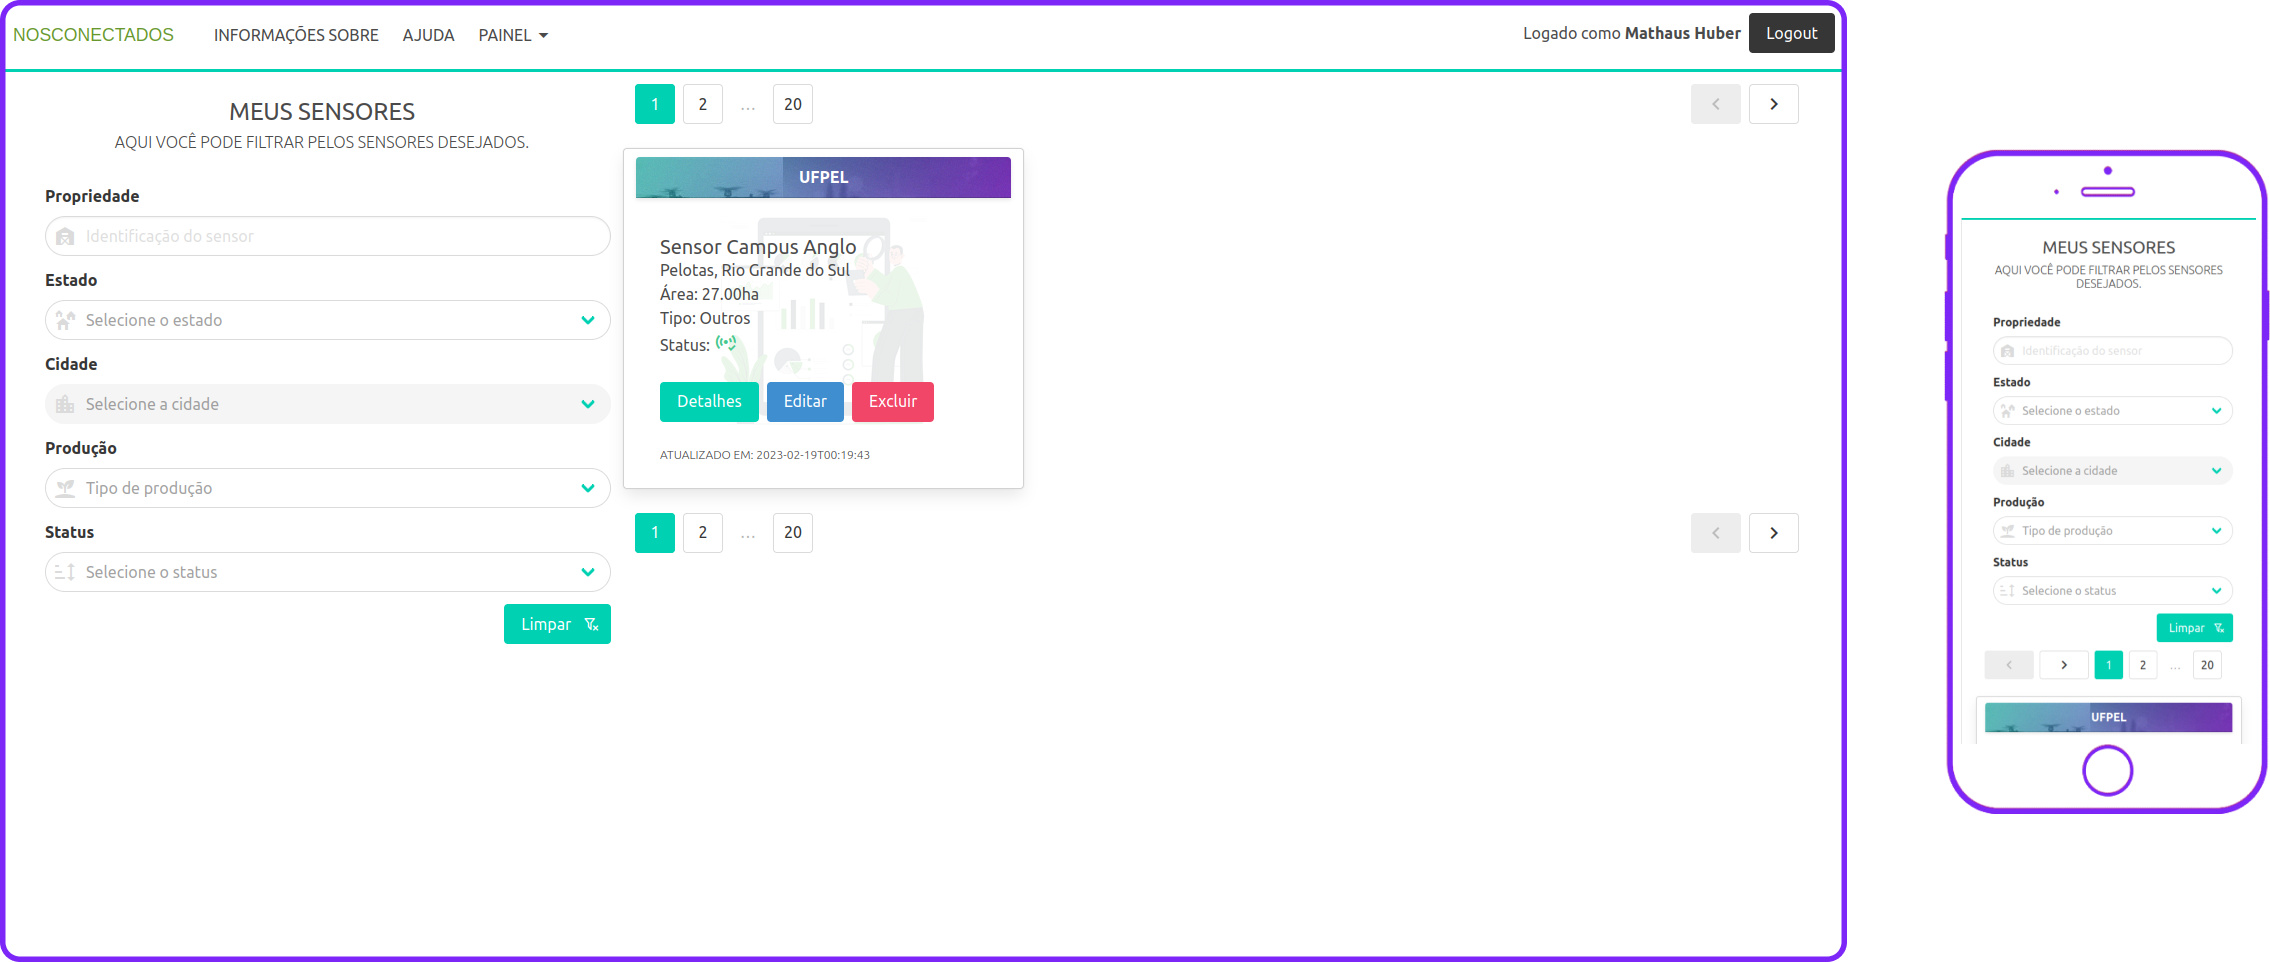
\includegraphics[scale=.2]{assets/meusensores.png}
  \caption{Página de sensores do usuário}
  \label{meusensores}
\end{figure}

\begin{figure}[htbp]
  \centering 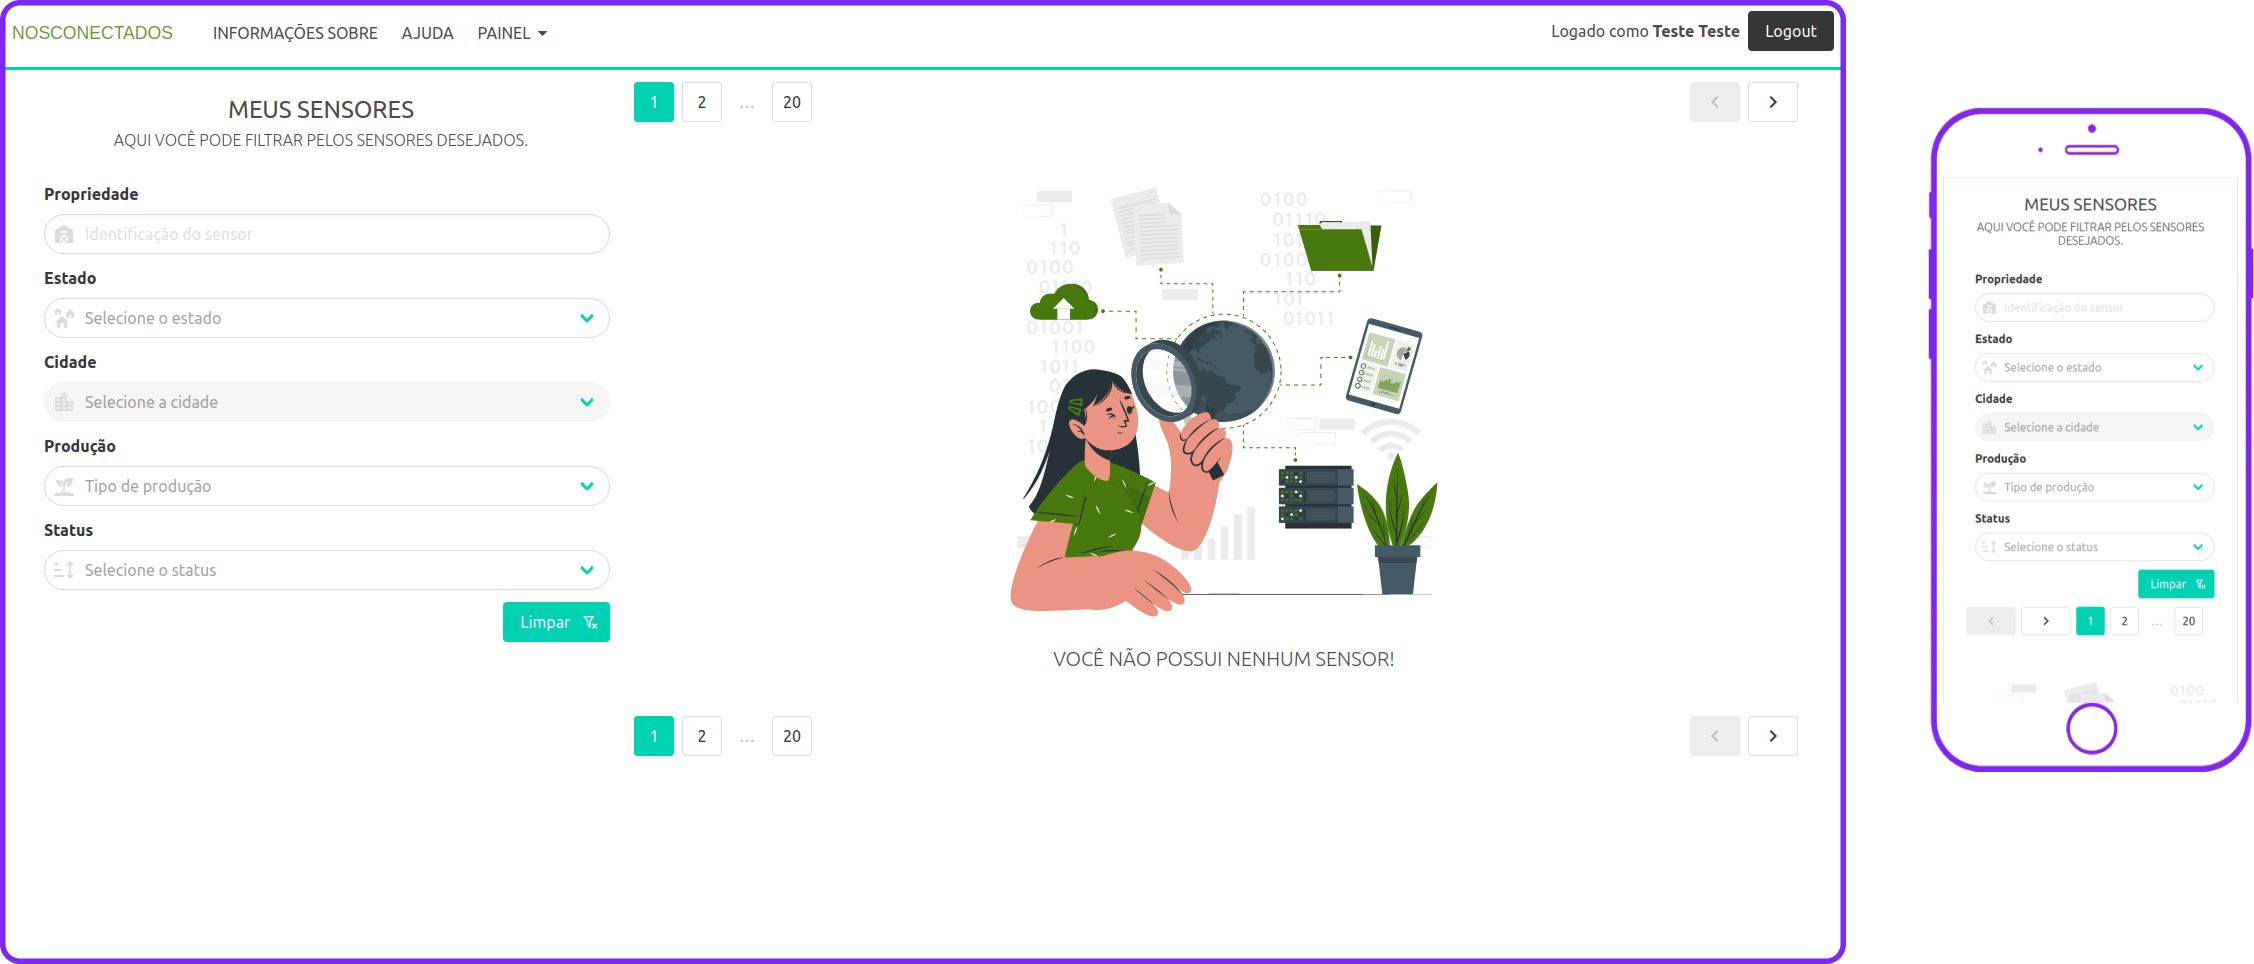
\includegraphics[scale=.2]{assets/meussensoresnull.png}
  \caption{Página de sensores do usuário quando não há sensores}
  \label{meusensoresnull}
\end{figure}

\begin{figure}[htbp]
  \centering 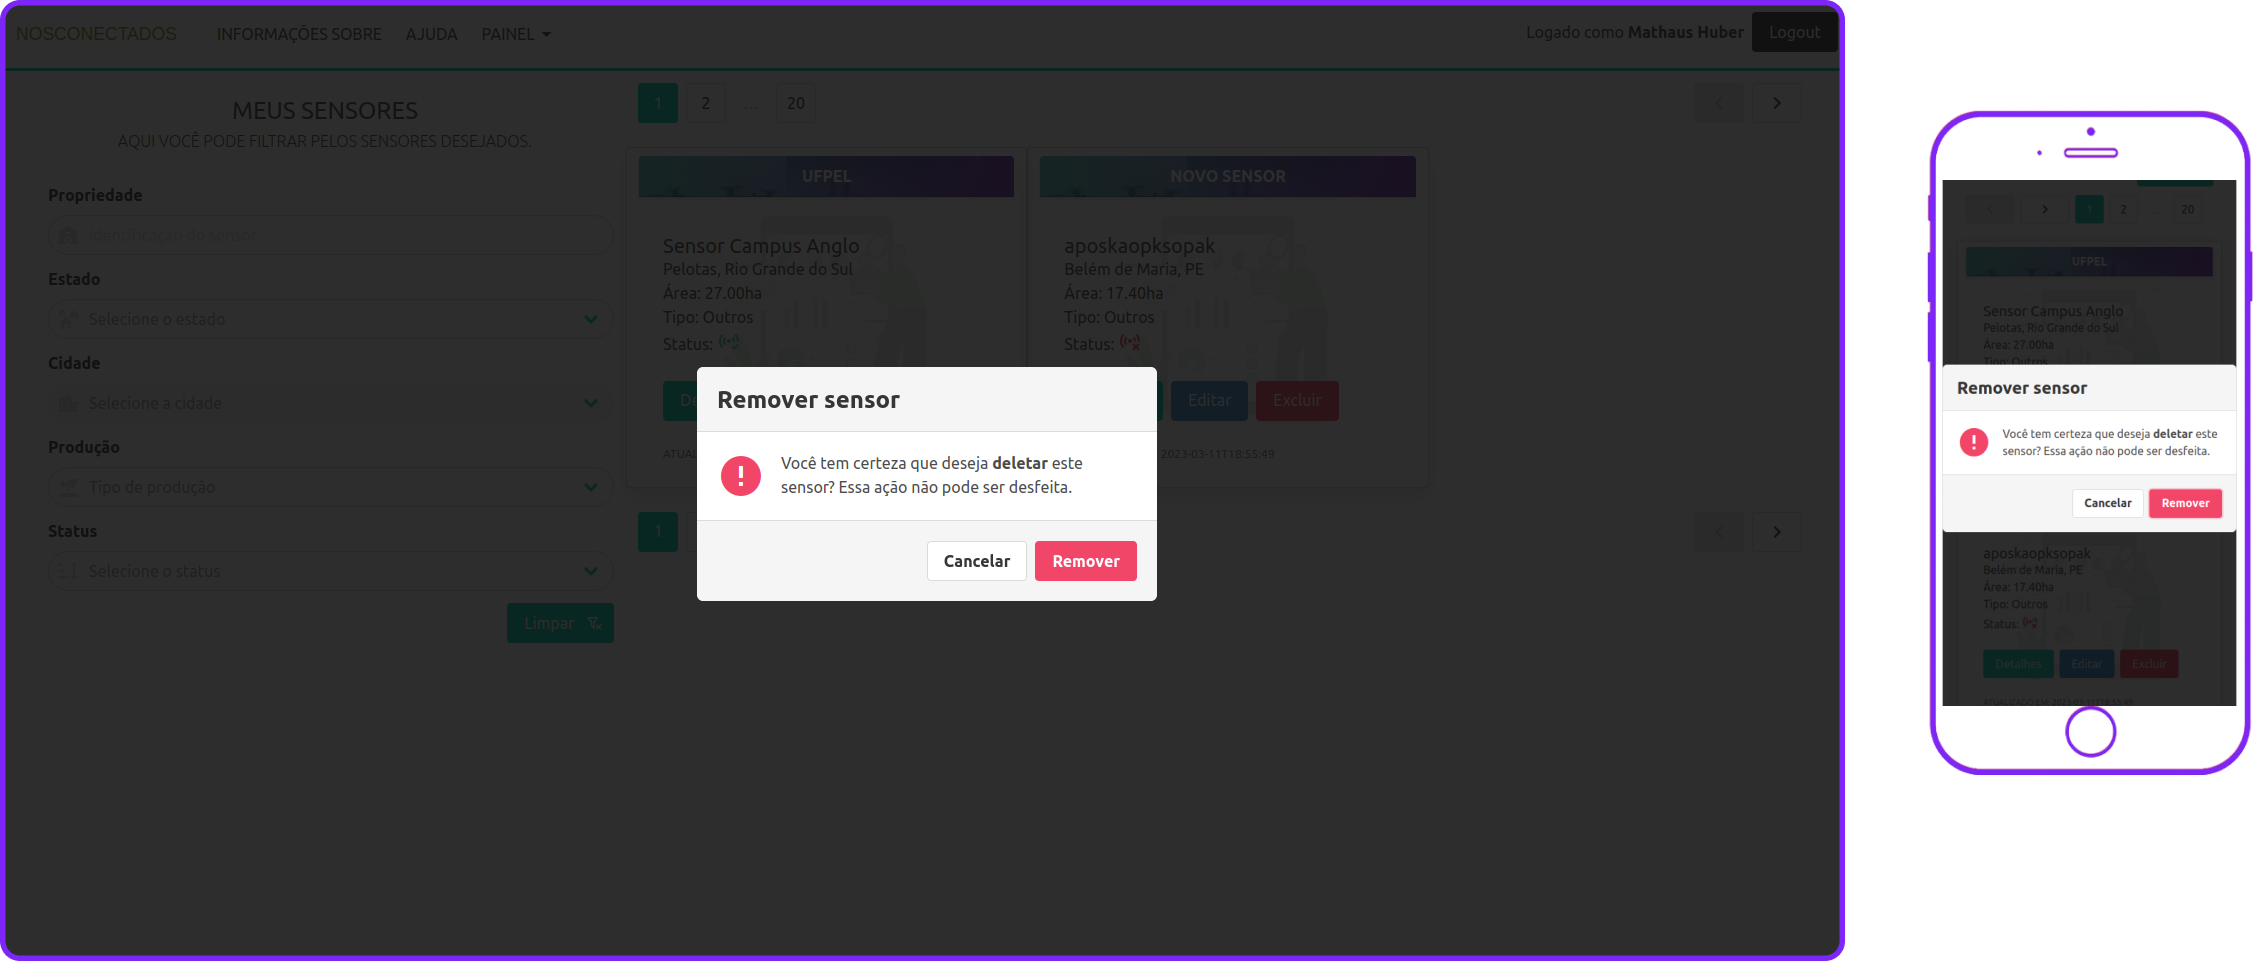
\includegraphics[scale=.2]{assets/meusensoresremover.png}
  \caption{Página de sensores do usuário ao solicitar remoção de sensor}
  \label{meusensoresremove}
\end{figure}
\newpage
\subsection{Administração}
A página de painel de administração é uma área restrita da plataforma, que somente pode ser acessada por usuários com privilégios de administrador. Ela oferece uma visão geral do sistema, incluindo informações importantes sobre o número de usuários e sensores cadastrados na plataforma. O menu lateral permite ao usuário acessar todas as informações armazenadas no banco de dados, tais como informações de usuário, informações de sensores, dados dos sensores e localizações dos usuários.

Uma das funcionalidades interessantes disponíveis na página de administração é a capacidade de exportar todos os dados da plataforma em um arquivo. Isso pode ser útil para análise de dados, para realizar backups dos dados ou para a migração para outra plataforma.

Além disso, a página "minha conta" \space permite aos administradores acessarem e gerenciarem suas próprias informações de perfil. Isso inclui a possibilidade de remover sua própria conta, o que pode ser útil em casos onde o administrador não deseja mais fazer parte do sistema. Vale ressaltar que, como administrador, não é possível remover sua conta através da página de edição de perfil como é feito pelos usuários normais.

A página de painel de administração é uma ferramenta poderosa e necessária para gerenciar e manter a plataforma em pleno funcionamento. Através dela, é possível acessar todas as informações importantes do sistema, o que permite tomar decisões baseadas em dados e realizar as ações necessárias para manter a plataforma operando de forma adequada. A figura \ref{painel} apresenta a visão inicial do painel de administração da plataforma.

\begin{figure}[htbp]
  \centering 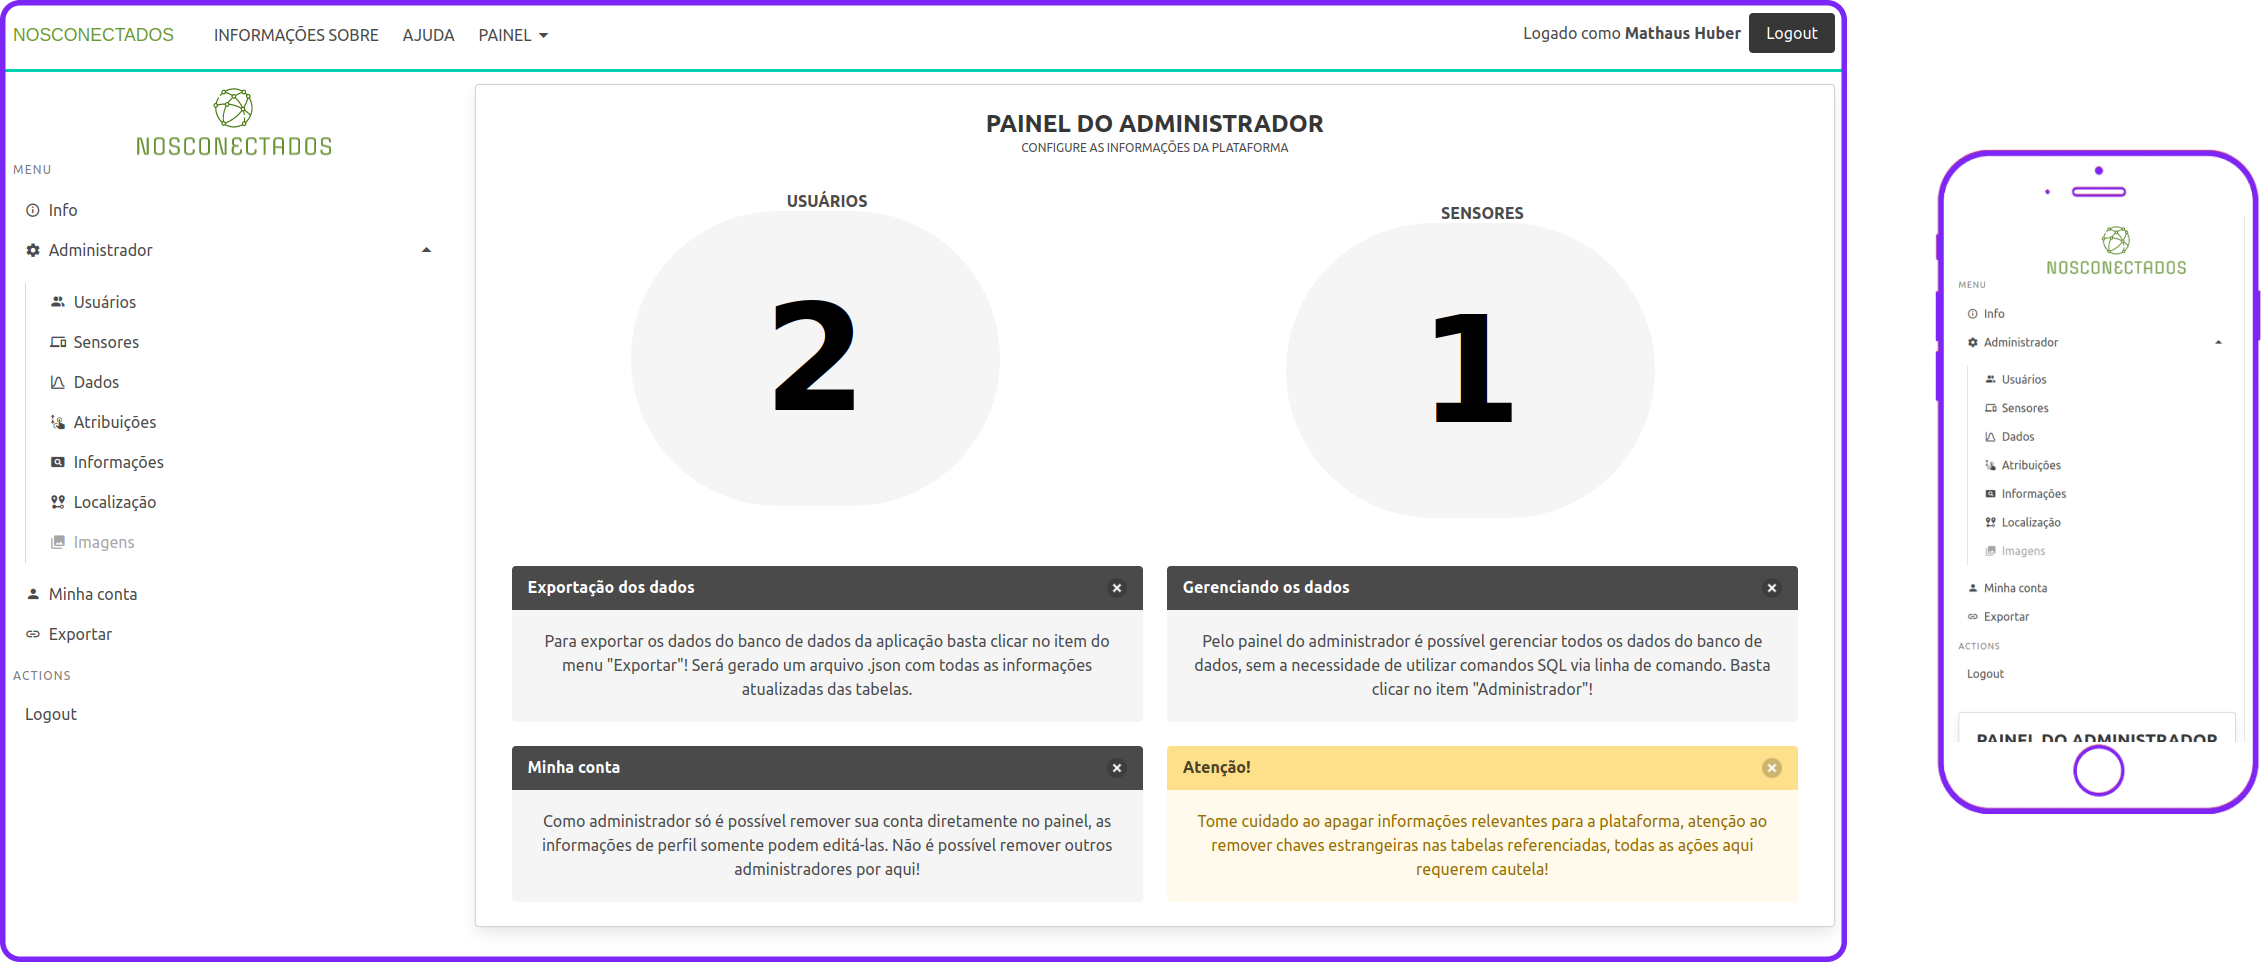
\includegraphics[scale=.2]{assets/painel.png}
  \caption{Página do painel de administração}
  \label{painel}
\end{figure}
\newpage
\subsubsection{Administração de usuários}
A seção de administração de usuários na página de painel do administrador permite que o administrador gerencie os usuários cadastrados na plataforma. Nesta seção, o administrador pode visualizar todas as informações dos usuários, como nome, telefone, cpf, data de criação da conta e nível de acesso.
Além disso, o administrador tem a opção de remover um usuário que não seja um administrador, mas não tem acesso à senha criptografada do usuário. Na figura \ref{adminusers} é possível ver como é a seção de administração de usuários dentro da página de administração da plataforma.
\begin{figure}[htbp]
  \centering 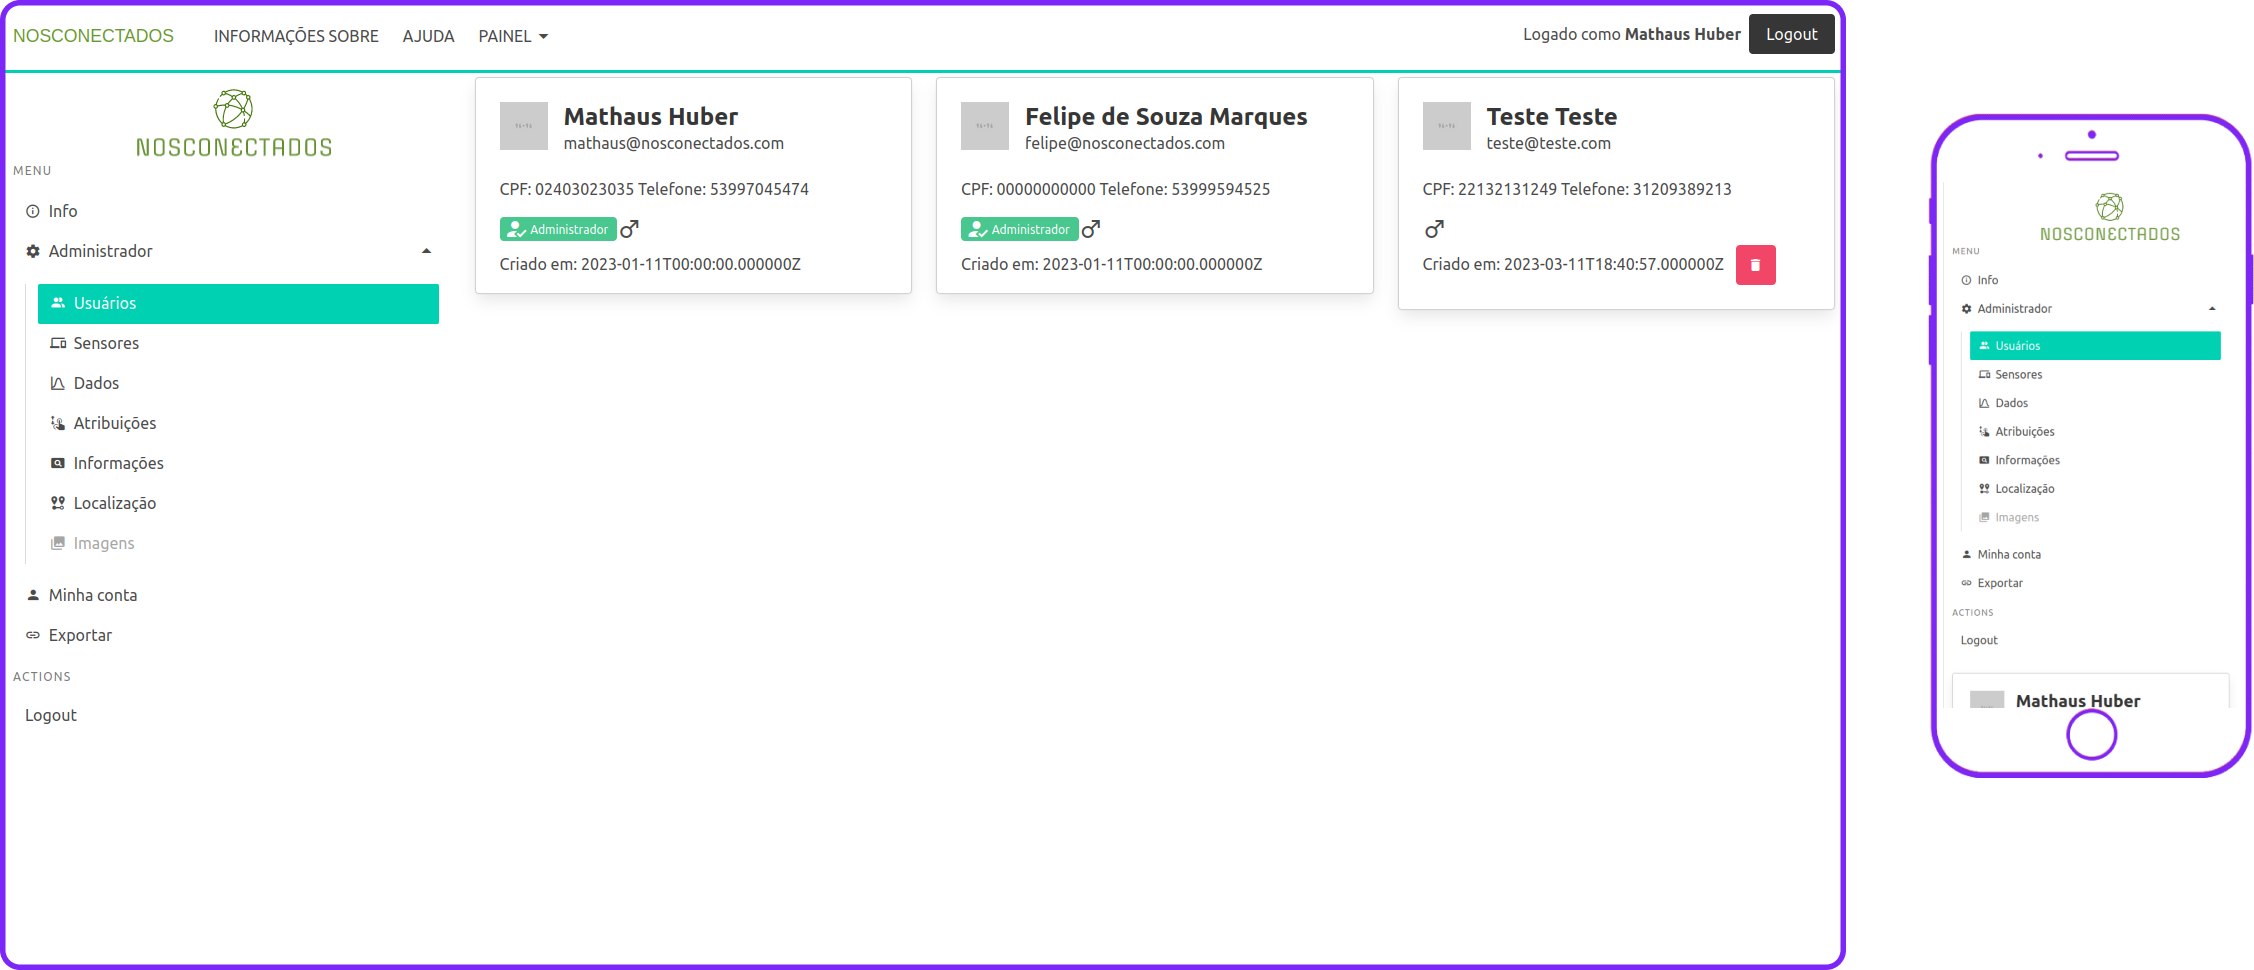
\includegraphics[scale=.2]{assets/painelusuarios.png}
  \caption{Página do painel de administração - administração de usuários}
  \label{adminusers}
\end{figure}
\subsubsection{Administração de sensores}
Na seção de administração de sensores, o administrador da plataforma tem acesso a algumas informações dos sensores cadastrados na plataforma. É possível visualizar as informações que são mais relevantes, como o nome do sensor, localização, tipo de sensor, estado do sensor, privacidade e a data de sua criação.

Além disso, na página de administração de sensores, o administrador tem a opção de remover sensores cadastrados na plataforma. Essa opção pode ser útil caso haja um sensor que não esteja mais em uso ou se houver algum problema com o sensor e for necessário substituí-lo.

É importante lembrar que a remoção de um sensor deve ser feita com cuidado, uma vez que essa ação pode impactar diretamente o monitoramento dos dados oriundos dos sensores restantes. Por isso, é importante avaliar com cuidado cada caso antes de remover um sensor da plataforma. A figura \ref{adminsensores} apresenta a seção de administração de sensores da plataforma, onde é possível gerenciar e visualizar informações importantes sobre os dispositivos cadastrados.

\begin{figure}[htbp]
  \centering 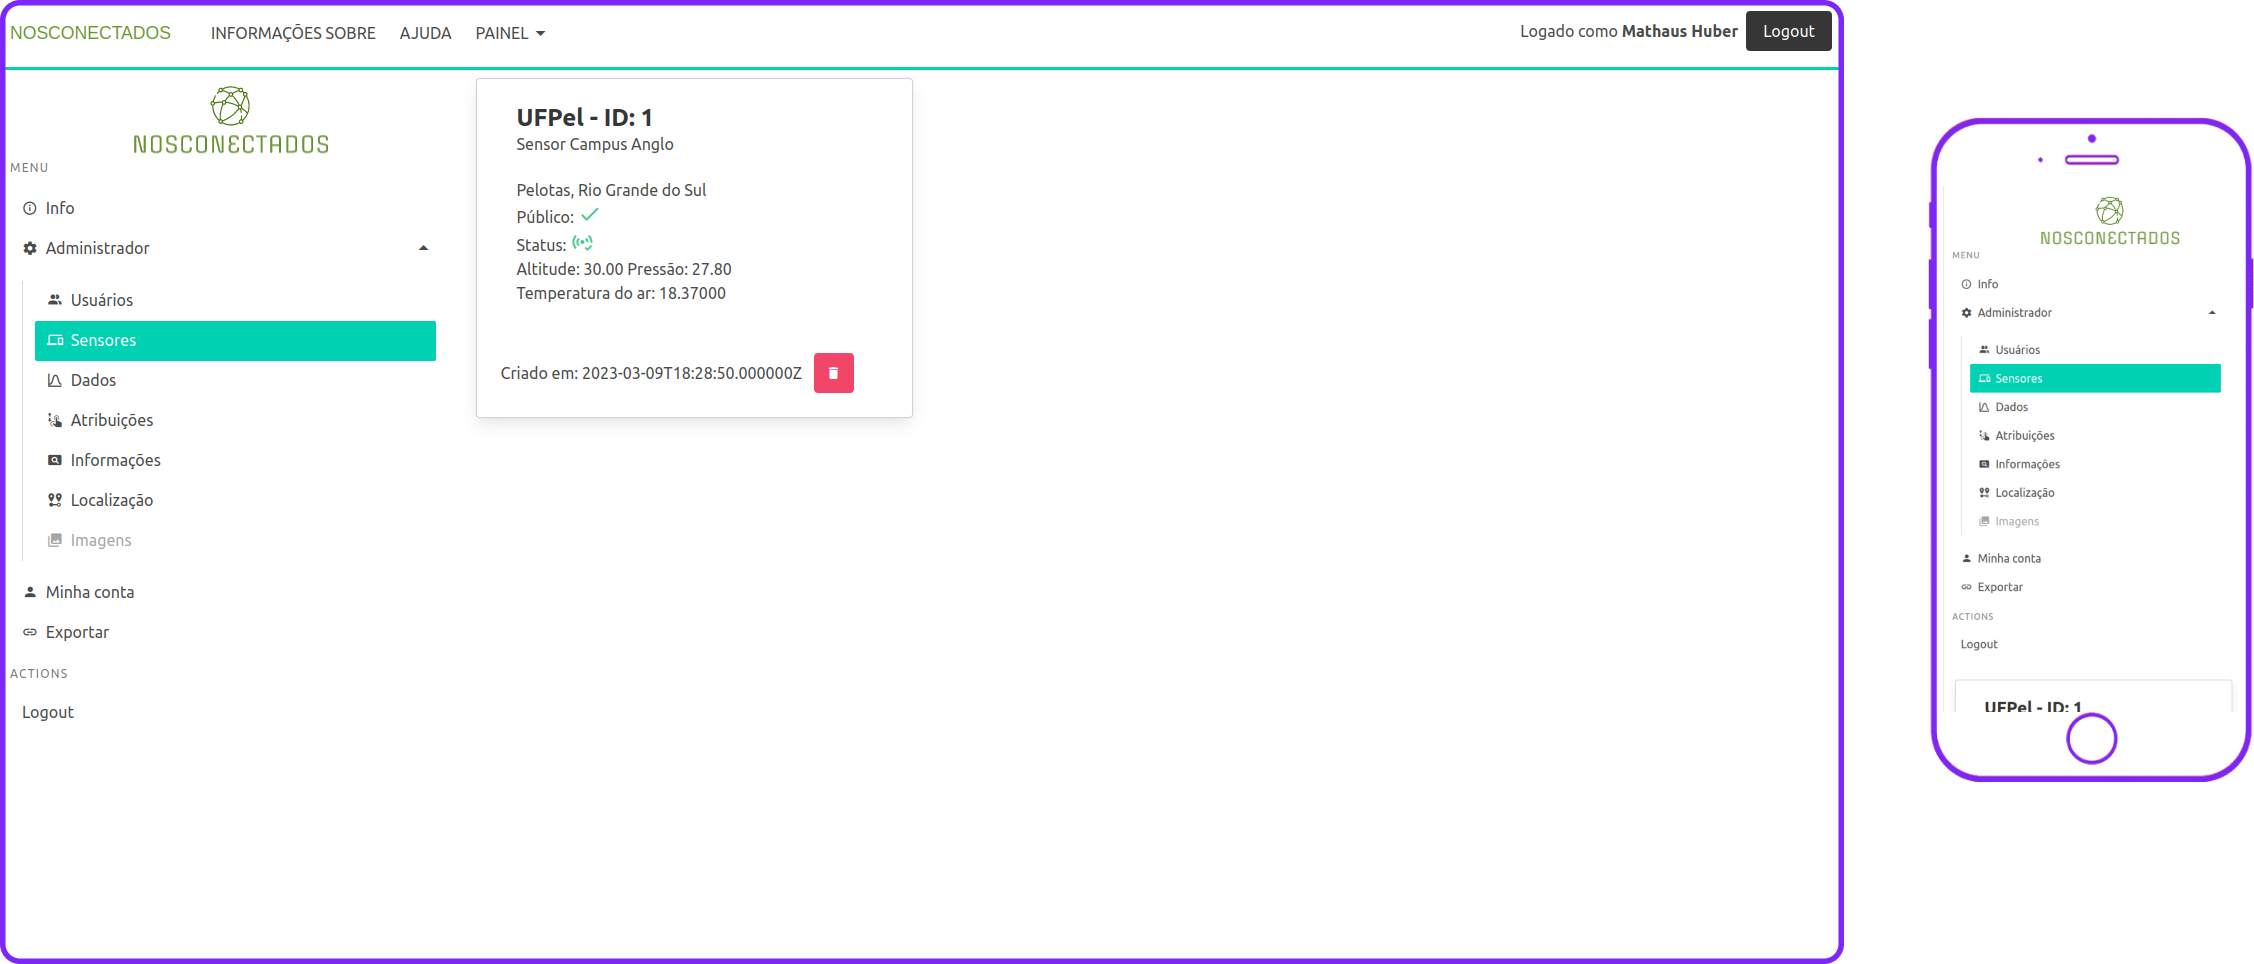
\includegraphics[scale=.2]{assets/painelsensores.png}
  \caption{Página do painel de administração - administração de sensores}
  \label{adminsensores}
\end{figure}
\newpage
\subsubsection{Administração de dados}
Na seção de administração de dados do painel do administrador, é possível visualizar todos os dados coletados pelos sensores da rede. Essa seção é essencial para garantir que a plataforma esteja funcionando corretamente e para analisar os dados coletados para identificar padrões e tendências. Os dados são exibidos em um card que inclui informações como o ID do sensor, a data e hora da leitura, e os dados gerados pelo sensor. A partir dessa tabela, o administrador pode selecionar e remover os dados que não são mais relevantes ou que podem estar comprometidos por algum motivo.

A remoção dos dados pode ser feita de forma individual. É importante lembrar que a remoção de dados deve ser feita com cuidado e sempre com base em critérios objetivos, a fim de evitar a perda de informações importantes para a análise dos dados. A figura \ref{admindados} apresenta a seção de administração dos dados da plataforma, onde é possível gerenciar e visualizar informações importantes sobre as leituras dos sensores cadastrados.

\begin{figure}[htbp]
  \centering 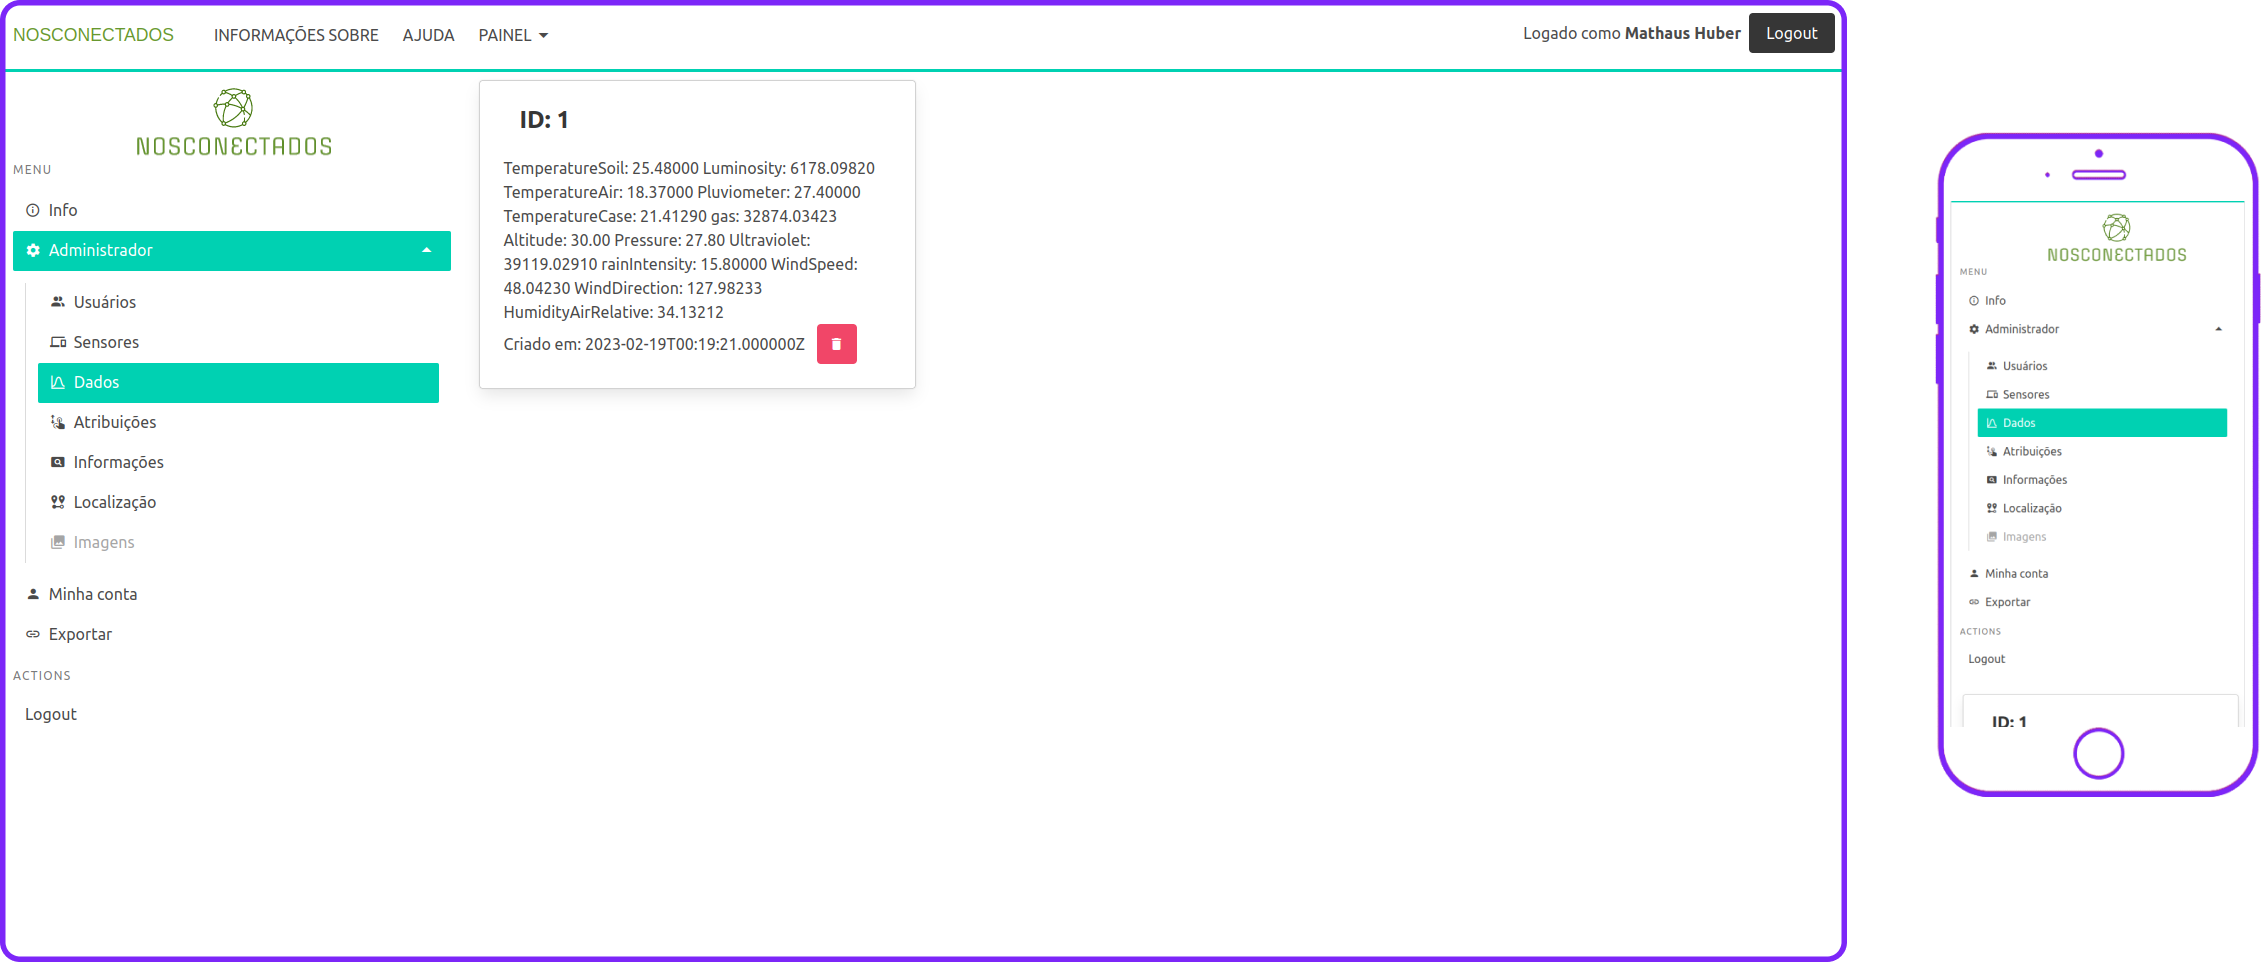
\includegraphics[scale=.2]{assets/paineldados.png}
  \caption{Página do painel de administração - administração de dados}
  \label{admindados}
\end{figure}
\newpage
\subsubsection{Administração de atribuições}
Nessa seção, o administrador tem acesso a todas as informações de atribuições dos sensores, incluindo quem são os administradores, patrocinadores e visualizadores de cada sensor.
Através dessa página, o administrador pode remover as atribuições de um sensor específico, caso necessário. Essa opção pode ser útil em casos em que um sensor está sendo utilizado por um patrocinador ou visualizador que não deveria mais ter acesso a ele. Na figura \ref{adminatrib} é possível ver como é a seção de administração de atribuições.
\begin{figure}[htbp]
  \centering 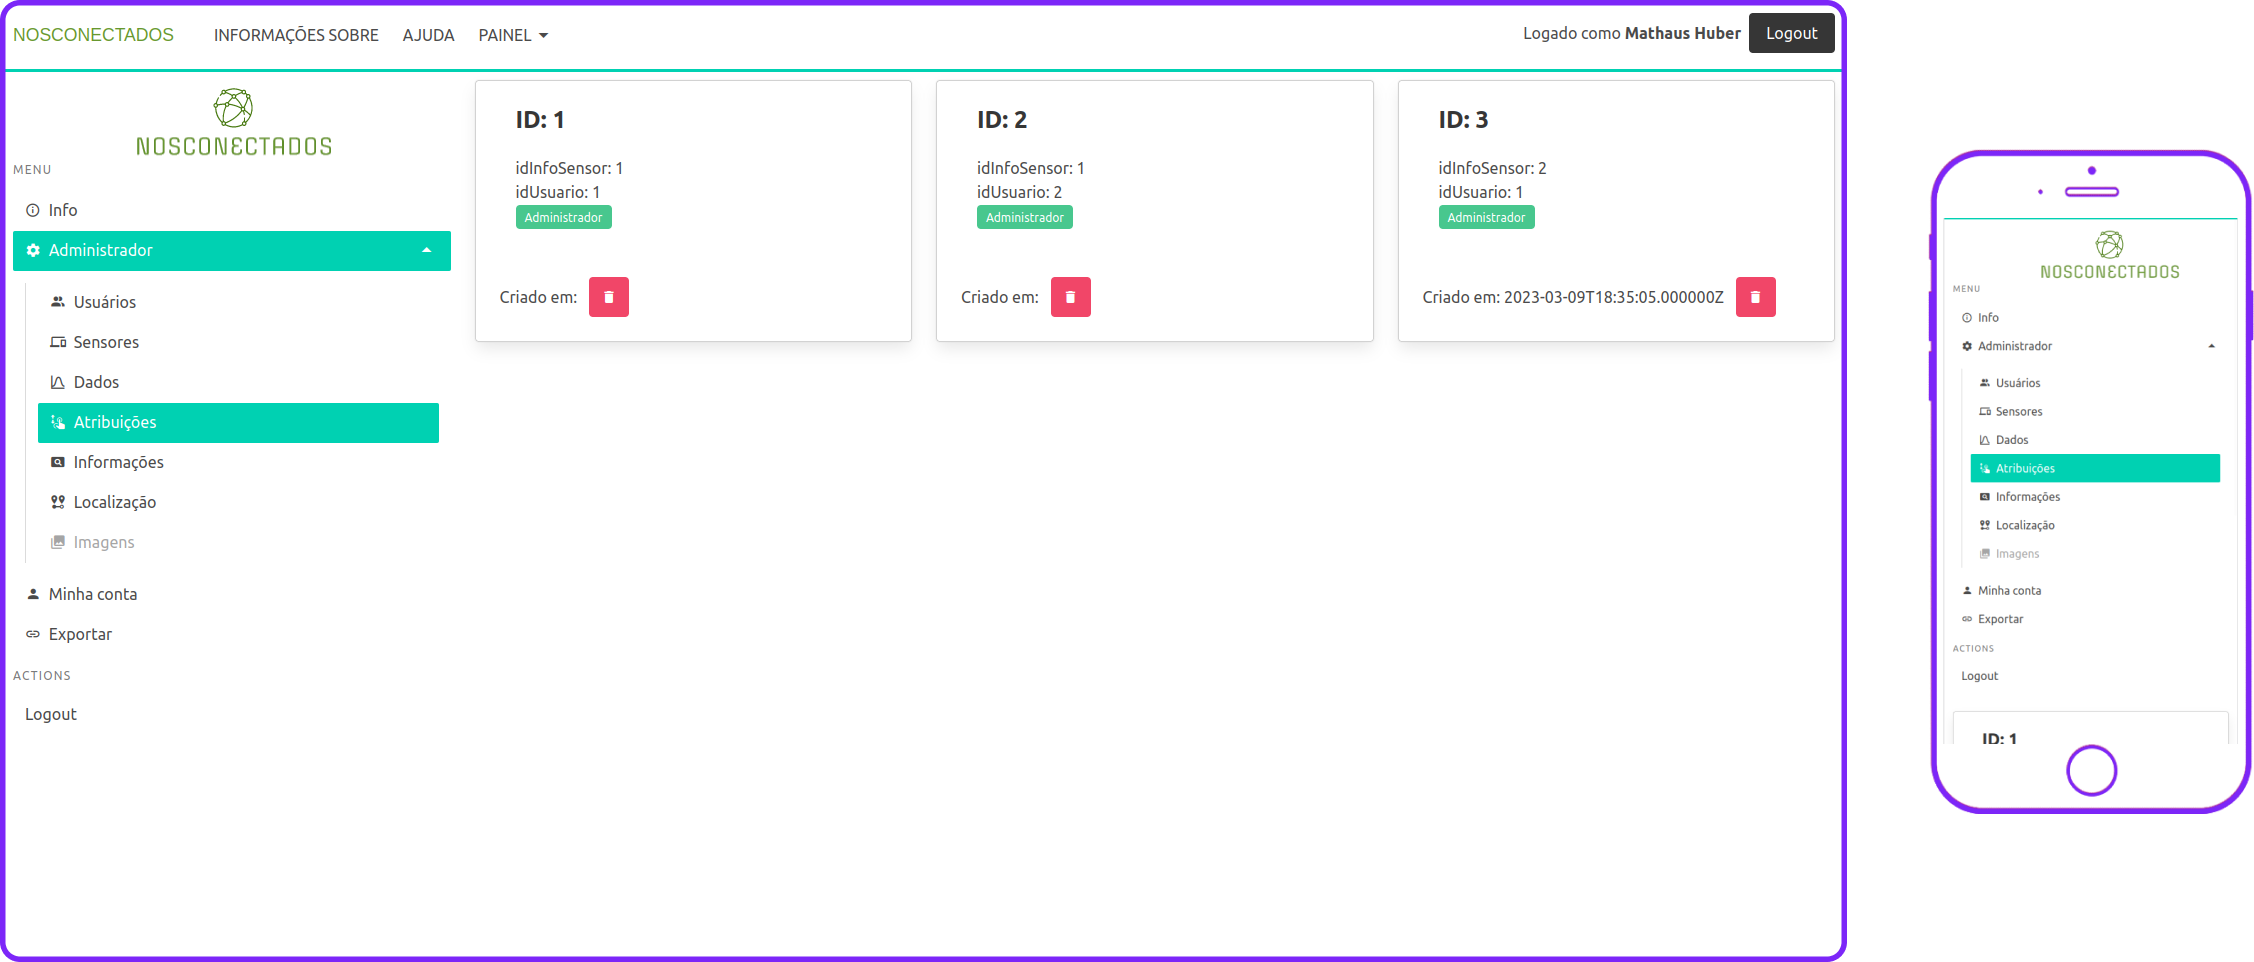
\includegraphics[scale=.2]{assets/painelatribuicao.png}
  \caption{Página do painel de administração - administração de atribuições}
  \label{adminatrib}
\end{figure}
\subsubsection{Administração de informações}
A seção de administração de informações no painel do administrador é essencial para gerenciar as informações dos sensores cadastrados na plataforma. Nesta seção, o administrador pode visualizar todas as informações dos sensores, tais como localização, cidade, estado, nome, tipo, privacidade, entre outros.

Além de visualizar essas informações, o administrador também pode remover as informações de um sensor, caso necessário. Isso pode ser útil, por exemplo, se uma informação estiver desatualizada ou se o sensor for removido da rede.

É importante destacar que as informações são diferentes dos dados coletados pelo sensor. Enquanto os dados são os valores medidos pelo sensor, as informações são as características do próprio sensor, como sua localização e nome. Essas informações são fundamentais para identificar e gerenciar os sensores na plataforma. Na figura figura \ref{admin_informacoes} é possível ver como é a seção de administração de informações dos sensores.

\begin{figure}[htbp]
  \centering \includegraphics[scale=.2]{assets/painelinformacoes.png}
  \caption{Página do painel de administração - administração de informações}
  \label{admin_informacoes}
\end{figure}
\subsubsection{Administração de localizações}
Na seção de administração de localizações, um administrador da plataforma pode visualizar as informações de localização de todos os usuários registrados e também pode remover qualquer localização que seja necessária. Essa seção do painel do administrador é extremamente importante para garantir a privacidade e segurança dos usuários da plataforma, pois permite que o administrador controle as informações de localização que são compartilhadas pelos usuários.

Ao acessar a seção de administração de localizações, o administrador pode visualizar uma lista de todas as localizações registradas pelos usuários. A partir daí, ele pode selecionar a localização específica que deseja remover e realizar essa ação com apenas alguns cliques. É importante ressaltar que o administrador deve ter o cuidado de garantir que as localizações sejam removidas apenas quando necessário, para evitar a perda de dados importantes. A seção de administração de localizações dos usuários pode ser visualizada na figura \ref{admin_localizacoes}, onde é possível gerenciar e visualizar informações importantes sobre a localização dos usuários cadastrados na plataforma.
\begin{figure}[htbp]
  \centering \includegraphics[scale=.2]{assets/painellocalizacoes.png}
  \caption{Página do painel de administração - administração de localizações}
  \label{admin_localizacoes}
\end{figure}

\subsubsection{Gerência da conta}
A seção "Minha Conta" na página de painel do administrador é uma ferramenta importante que permite que o próprio administrador gerencie suas informações pessoais e controle o acesso à sua conta na plataforma. Essa seção é exclusiva para administradores, sendo acessível somente a partir da página de painel de administração.

Através dessa seção, o administrador pode visualizar seus dados pessoais, incluindo nome, sobrenome, endereço de e-mail, senha (criptografada) e outras informações relevantes. O administrador também pode editar suas informações pessoais através de um botão de edição de perfil, que o leva para a página de edição de perfil.

Além disso, o administrador também pode remover sua conta através dessa seção. Esse processo é irreversível e todas as informações relacionadas à conta do administrador serão apagadas permanentemente. Por esse motivo, é importante que o administrador esteja ciente das consequências da exclusão da sua conta antes de tomar essa decisão. A página de dados pessoais de um usuário administrador pode ser visualizada na figura \ref{gerencia_conta}.
\begin{figure}[htbp]
  \centering \includegraphics[scale=.2]{assets/painelconta.png}
  \caption{Página do painel de administração - gerência da conta}
  \label{gerencia_conta}
\end{figure}
\newpage
\subsubsection{Exportação de dados}
Essa seção permite que o administrador da plataforma obtenha todas as informações armazenadas no banco de dados em um arquivo. Isso pode ser útil para análises posteriores, armazenamento de backups, entre outras finalidades.

Para extrair os dados, o administrador precisa acessar a seção correspondente no painel de administração e selecionar os parâmetros que deseja incluir no arquivo de extração, como intervalo de tempo, tipo de dado, sensor, entre outros. Após selecionar os parâmetros desejados, basta clicar no botão "Exportar" e aguardar o processamento do arquivo.

É importante lembrar que a extração de dados deve ser feita com cuidado, pois pode ser uma tarefa complexa e pode consumir recursos do servidor. Além disso, é necessário que o administrador tenha permissões adequadas para acessar essa funcionalidade e que tome as precauções necessárias para manter a segurança dos dados extraídos. A figura \ref{exportacao} exemplifica o processo de exportação de dados do banco de dados, diretamente pelo painel do administrador.

\begin{figure}[htbp]
  \centering \includegraphics[scale=.2]{assets/painelexportar.png}
  \caption{Página do painel de administração - exportação de dados}
  \label{exportacao}
\end{figure}
\newpage


\chapter{Conclusão}
Com base nos objetivos traçados neste trabalho, conclui-se que a plataforma web NosConectados é uma solução inovadora para o monitoramento de dados oriundos de redes de sensores sem fio, com possibilidade de aplicação em diversos setores, como agricultura digital, pesquisas acadêmicas, smartcities e smartcampus, entre outros.


A criação de dashboards e APIs permite a visualização e a integração dos dados coletados de diferentes tipos de sensores, incluindo dados de telemetria, possibilitando a tomada de decisões mais assertivas e a melhoria dos processos produtivos.
Além disso, o fluxo constante de dados permite a geração de séries históricas que podem ser utilizadas para análises preditivas, auxiliando na tomada de decisões estratégicas.

A plataforma NosConectados, portanto, apresenta um grande potencial para a inovação tecnológica, aprimorando a eficiência e a competitividade do mercado. Com isso, espera-se que este trabalho possa contribuir para o avanço da tecnologia da Internet das Coisas e para o desenvolvimento de novas soluções que possam ajudar na construção de um futuro mais conectado e inteligente.
% Bibliografia http://liinwww.ira.uka.de/bibliography/index.html um
% site que cataloga no formato bibtex a bibliografia em computacao
% \bibliography{nomedoarquivo.bib} (sem extensao)
% \bibliographystyle{formato.bst} (sem extensao)

\bibliographystyle{abnt}
\bibliography{bibliografia} 

% Apêndices (Opcional) - Material produzido pelo autor

% Anexos (Opcional) - Material produzido por outro


% Faz a capa do CDROM
% \makecover

\end{document}

